\documentclass[11pt,]{book}
\usepackage{lmodern}
\usepackage{amssymb,amsmath}
\usepackage{ifxetex,ifluatex}
\usepackage{fixltx2e} % provides \textsubscript
\ifnum 0\ifxetex 1\fi\ifluatex 1\fi=0 % if pdftex
  \usepackage[T1]{fontenc}
  \usepackage[utf8]{inputenc}
\else % if luatex or xelatex
  \ifxetex
    \usepackage{mathspec}
  \else
    \usepackage{fontspec}
  \fi
  \defaultfontfeatures{Ligatures=TeX,Scale=MatchLowercase}
    \setmainfont[]{Calibri}
\fi
% use upquote if available, for straight quotes in verbatim environments
\IfFileExists{upquote.sty}{\usepackage{upquote}}{}
% use microtype if available
\IfFileExists{microtype.sty}{%
\usepackage{microtype}
\UseMicrotypeSet[protrusion]{basicmath} % disable protrusion for tt fonts
}{}
\usepackage[margin=1in]{geometry}
\usepackage{hyperref}
\PassOptionsToPackage{usenames,dvipsnames}{color} % color is loaded by hyperref
\hypersetup{unicode=true,
            pdftitle={Ontwerp van een early-warning meetnet voor droogte in natuurgebieden},
            pdfauthor={Jan Wouters, Floris Vanderhaeghe},
            colorlinks=true,
            linkcolor=link.colour,
            citecolor=link.colour,
            urlcolor=link.colour,
            breaklinks=true}
\urlstyle{same}  % don't use monospace font for urls
\usepackage{longtable,booktabs}
\usepackage{graphicx,grffile}
\makeatletter
\def\maxwidth{\ifdim\Gin@nat@width>\linewidth\linewidth\else\Gin@nat@width\fi}
\def\maxheight{\ifdim\Gin@nat@height>\textheight\textheight\else\Gin@nat@height\fi}
\makeatother
% Scale images if necessary, so that they will not overflow the page
% margins by default, and it is still possible to overwrite the defaults
% using explicit options in \includegraphics[width, height, ...]{}
\setkeys{Gin}{width=\maxwidth,height=\maxheight,keepaspectratio}
\IfFileExists{parskip.sty}{%
\usepackage{parskip}
}{% else
\setlength{\parindent}{0pt}
\setlength{\parskip}{6pt plus 2pt minus 1pt}
}
\setlength{\emergencystretch}{3em}  % prevent overfull lines
\providecommand{\tightlist}{%
  \setlength{\itemsep}{0pt}\setlength{\parskip}{0pt}}
\setcounter{secnumdepth}{5}
% Redefines (sub)paragraphs to behave more like sections
\ifx\paragraph\undefined\else
\let\oldparagraph\paragraph
\renewcommand{\paragraph}[1]{\oldparagraph{#1}\mbox{}}
\fi
\ifx\subparagraph\undefined\else
\let\oldsubparagraph\subparagraph
\renewcommand{\subparagraph}[1]{\oldsubparagraph{#1}\mbox{}}
\fi

%%% Use protect on footnotes to avoid problems with footnotes in titles
\let\rmarkdownfootnote\footnote%
\def\footnote{\protect\rmarkdownfootnote}

%%% Change title format to be more compact
\usepackage{titling}

% Create subtitle command for use in maketitle
\providecommand{\subtitle}[1]{
  \posttitle{
    \begin{center}\large#1\end{center}
    }
}

\setlength{\droptitle}{-2em}

  \title{Ontwerp van een early-warning meetnet voor droogte in natuurgebieden}
    \pretitle{\vspace{\droptitle}\centering\huge}
  \posttitle{\par}
    \author{Jan Wouters, Floris Vanderhaeghe}
    \preauthor{\centering\large\emph}
  \postauthor{\par}
      \predate{\centering\large\emph}
  \postdate{\par}
    \date{Versie 2019-11-18 23:58:24}

% definition of INBO colours
\RequirePackage{xcolor}
\definecolor{box.colour}{RGB}{229, 229, 229}
\definecolor{link.colour}{RGB}{192, 67, 132}

% allow landscape pages and define commands that work with pandoc
\RequirePackage{lscape}
\newcommand{\blandscape}{\begin{landscape}}
\newcommand{\elandscape}{\end{landscape}}

% allow use of FloatBarrier
\RequirePackage{placeins}

% definition of block, alertblock and exampleblock
\RequirePackage{mdframed}

\newenvironment{block}[2][]{%
  \begin{mdframed}[backgroundcolor=box.colour]
  \textbf{#2}%

}
{
  \end{mdframed}
}
\usepackage{booktabs}
\usepackage{longtable}
\usepackage{array}
\usepackage{multirow}
\usepackage{wrapfig}
\usepackage{float}
\usepackage{colortbl}
\usepackage{pdflscape}
\usepackage{tabu}
\usepackage{threeparttable}
\usepackage{threeparttablex}
\usepackage[normalem]{ulem}
\usepackage{makecell}
\usepackage{xcolor}

\begin{document}
\maketitle

{
\hypersetup{linkcolor=black}
\setcounter{tocdepth}{2}
\tableofcontents
}
\chapter{Inleiding}\label{inleiding}

\begin{quote}
Het basisidee van het early-warning meetnet droogte is om in
natuurgebieden een vooraf gekozen aantal meetpunten zo goed mogelijk
ruimtelijk gebalanceerd te selecteren, rekening houdende met mogelijke
verschillen in het gedrag van het grond/oppervlaktewaterpeil t.a.v. een
neerslagtekort. Voor deze meetpunten kan op basis van actuele informatie
een indicator (cfr. droogte-indicator) worden berekend.
\end{quote}

Het project omhelst :

\begin{itemize}
\tightlist
\item
  uitwerking van een methodiek die een ruimtelijk gebalanceerde selectie
  van actuele en potentiële meetlocaties mogelijk maakt
\item
  bepalen van referentiewaarden voor de actuele meetlocaties
\end{itemize}

Met natuurgebieden worden hier alle locaties met grondwaterafhankelijke
habitattypes en rbb's bedoeld, gelegen binnen of buiten het Natura 2000
netwerk. In overeenstemming met het meetnet natuurlijk milieu (MNM) voor
de milieudruk `verdroging via grondwater' worden volgende habitattypen
en rbb's als grondwaterafhankelijk beschouwd (tabel \ref{tab:gw-typen}).
Hierna worden deze typen afgekort tot gaHT.

\begin{table}

\caption{\label{tab:gw-typen}grondwaterafhankelijke habitattypen en rbb's}
\centering
\begin{tabular}[t]{l|l|r}
\hline
habitat(sub)type of rbb & (verkorte) naam & GT-groep: nummer\\
\hline
1310\_pol & binnendijkse zeekraalvegetatie & 3\\
\hline
1310\_zk & buitendijks laag schor & 1\\
\hline
1310\_zv & buitendijks hoog schor & 1\\
\hline
1320 & schorren met slijkgras & 1\\
\hline
1330\_da & buitendijkse schor & 1\\
\hline
1330\_hpr & zilte graslanden & 3\\
\hline
2130\_had & kalkarme duingraslanden & 5\\
\hline
2130\_hd & kalkrijke duingraslanden & 5\\
\hline
2160 & duindoornstruwelen & 4\\
\hline
2170 & kruipwilgstruwelen & 4\\
\hline
2180 & duinbossen & 4\\
\hline
2190\_mp & duinpannen (kalkrijk) & 2\\
\hline
2190\_overig & vochtige duinvalleien - overige vegetaties & 4\\
\hline
3270 & voedselrijke slikoevers met bepaalde eenjarige planten & 1\\
\hline
4010 & vochtige heide & 3\\
\hline
6230\_hmo & vochtige heischrale graslanden & 4\\
\hline
6410\_mo & blauwgrasland & 3\\
\hline
6410\_ve & veldrusgrasland & 3\\
\hline
6430\_bz & nitrofiele boszoom & 5\\
\hline
6430\_hf & moerasspirearuigte & 3\\
\hline
6430\_hw & ruigte en zoom met harig wilgenroosje & 3\\
\hline
6430\_mr & ruiger rietland & 2\\
\hline
6510\_hua & habitatwaardig vossenstaartgrasland & 4\\
\hline
6510\_hus & pimpernelgrasland & 4\\
\hline
7140\_base & basenrijk trilveen & 1\\
\hline
7140\_meso & circum-neutraal overgangsveen & 1\\
\hline
7140\_mrd & rietland op drijftillen & 1\\
\hline
7140\_oli & zuur overgangsveen & 1\\
\hline
7150 & pioniervegetaties met snavelbiezen & 3\\
\hline
7210 & galigaanmoerassen & 1\\
\hline
7230 & alkalisch laagveen & 1\\
\hline
9130\_end & atlantisch neutrofiel beukenbos & 4\\
\hline
9130\_fm & midden-Europese neutrofiel beukenbos & 5\\
\hline
9160 & eiken-haagbeukenbossen & 4\\
\hline
9190 & oude eiken-berkenbossen & 5\\
\hline
91E0\_sf & wilgenvloedbos & 3\\
\hline
91E0\_va & beekbegeleidend bos & 4\\
\hline
91E0\_vc & goudveil-essenbos & 1\\
\hline
91E0\_vm & mesotroof broekbos & 1\\
\hline
91E0\_vn & ruigt-elzenbos & 3\\
\hline
91E0\_vo & oligotroof broekbos & 1\\
\hline
91F0 & hardhoutooibossen & 4\\
\hline
rbbhc & dotterbloemgrasland & 3\\
\hline
rbbhf & moerasspirearuigte met graslandkenmerken & 3\\
\hline
rbbhfl & natte ruigte met grote wederik en hennegras & 3\\
\hline
rbbkam & kamgrasland & 5\\
\hline
rbbmc & grote zeggenvegetatie & 2\\
\hline
rbbmr & rietland en andere vegetatie van het rietverbond & 2\\
\hline
rbbms & kleine zeggenvegetatie niet vervat in 7140 & 2\\
\hline
rbbppm & structuurrijk, oud bestand van grove den & 5\\
\hline
rbbsf & moerasbos van breedbladige wilgen & 3\\
\hline
rbbsm & gagelstruweel & 3\\
\hline
rbbso & vochtig wilgenstruweel op venige of zure grond & 3\\
\hline
rbbvos & grote vossenstaartgrasland & 4\\
\hline
rbbzil & zilverschoongrasland & 3\\
\hline
\end{tabular}
\end{table}

Een min of meer ruimtelijk gebalanceerde set van bestaande meetlocaties
maakt het mogelijk om conclusies te trekken die benaderend
representatief zijn voor heel het studiegebied. Via deze benadering
wordt ook een goede synergie bekomen met de implementatie van de zg.
`overgangsfase' van het grondwatermeetnet in MNM (Vanderhaeghe \emph{et
al.}, \protect\hyperlink{ref-vanderhaeghe_meetnetten_2018}{2018}:
hoofdstuk 6).

Er wordt met dit meetnet niet beoogd om specifiek voor elk gaHT te
bepalen of het aan droogte onderhevig is. Het meetnet wil een globale
uitspraak faciliteren. Hierbij achten we het belangrijk om rekening te
houden met de mogelijke verschillen in responstijd (`hoe snel laat een
neerslagtekort zich voelen in een wijziging van het grondwaterpeil') op
droogte. De responstijd is onder meer afhankelijk van de
landschappelijke positie. Vegetaties die voorkomen in
lokaal-grondwatergevoede systemen zullen sneller een droogte gewaar
worden dan vegetaties die gebonden zijn aan (regionale) systemen met een
permanente aanvoer van grondwater. We veronderstellen hierbij dat er een
relatie bestaat tussen het hydrologisch regime en de responstijd:
permanent grondwatergevoede systemen reageren trager dan systemen met
een tijdelijke of zwakke grondwatervoeding.

We vertrekken hiervoor van de 5-delige indeling in grondwatertypegroepen
(GT-groep) die toegepast wordt in het MNM (tabel \ref{tab:GTgroepen}).
In de vorige tabel \ref{tab:gw-typen}) is weergegeven tot welke GT-groep
een gaHT gerekend wordt.

\begin{table}

\caption{\label{tab:GTgroepen}Grondwatertype-groepen}
\centering
\begin{tabular}[t]{r|l}
\hline
GT-groep: nummer & GT-groep: naam\\
\hline
1 & types van zeer nat milieu\\
\hline
2 & types van nat milieu\\
\hline
3 & types van matig nat milieu\\
\hline
4 & types van vochtig milieu\\
\hline
5 & types van droog milieu\\
\hline
\end{tabular}
\end{table}

\emph{GT-groep 5 bundelt grondwaterafhankelijke HT die zodanig breed
gedefinieerd zijn dat ze op sommige locaties grondwatergevoed zijn, maar
soms tot meestal niet. }\textbf{De vraag is of we deze groep
meenemen.}\_ \emph{\textbf{We zijn voorstander om deze wel mee te
nemen.}} \emph{\textbf{Het voordeel van deze groep is dat ze
vermoedelijk het snelst op droogte zal reageren.}} \emph{\textbf{Ze
heeft echter ook een nadeel, nl. dat je bij het uitzetten van een nieuw
punt niet op voorhand weet of het wel grondwaterafhankelijk is.}}\\
De GT-groepen lenen zich heel goed om een stratificatie uit te voeren op
basis van de verwachte responssnelheid van een locatie op droogte. De
permanent gevoede locaties (GT-groep 1) zullen naar verwachting trager
reageren dan de tijdelijk of zwak gevoede locaties. Door een
stratificatie over de GT-groepen toe te passen kan een \emph{zekere}
\textbf{\emph{(nog af te spreken)}} balans worden verzekerd.
\textbf{\emph{Een stratificatie laat toe om een globale uitspraak te
doen.}} \textbf{\emph{We raden echter ook aan in de beoordeling elke
GT-groep apart mee te nemen, omdat ze verschillende signalen zullen
geven.}}

\chapter{Methode}\label{methode}

\section{Ontwerp van het meetnet}\label{ontwerp-van-het-meetnet}

\subsection{Ruimtelijke selectie van
rastercellen}\label{ruimte-sel-raster}

Idealiter liggen de meetlocaties ruimtelijk gebalanceerd, omdat dit de
beste garantie biedt dat de gebeurtenissen die zich op deze locaties
voordoen, representatief zijn voor het hele gebied.\\
Men kan een ruimtelijk gebalanceerde set opbouwen door de verspreiding
van de GT-groepen over een fijn GRTS-raster\footnote{GRTS-design =
  Generalized Random Tessellation Stratified design. Een GRTS-raster is
  hiervoor de basis.} te leggen.

Een GRTS-raster is een raster, waarbij een willekeurig gekozen subset
van opeenvolgende genummerde punten steeds een ruimtelijk gebalanceerde
set vormen. Kiezen we een willekeurig nummer en vormen we een reeks
opeenvolgende punten ter grootte van ons vooraf gekozen aantal, dan
verkrijgen we steeds een goed ruimtelijk gebalanceerde set.\\
Kees denkt dan wel dat hij klaar is, het is jammergenoeg niet zo
eenvoudig.

\begin{enumerate}
\def\labelenumi{\arabic{enumi}.}
\tightlist
\item
  De kans dat op een dergelijk punt zich een bestaand grondwatermeetpunt
  bevindt, is namelijk weinig realistisch. Het karakteriseren van een
  nieuwe locatie, zodat het kan ingezet worden in het meetnet, vergt
  verschillende jaren grondwatermetingen.
\item
  We hebben ook geen controle over de verdeling van de punten over de
  verschillende grondwatertypegroepen, die verschillend op droogte
  kunnen reageren.
\end{enumerate}

We kunnen om deze redenen geen zuiver ruimtelijk gebalanceerde set
opbouwen.

De drie hoofdfactoren waar we bij het ontwerp mee rekening houden, zijn:

\begin{itemize}
\tightlist
\item
  We willen zoveel mogelijk een ruimtelijk gebalanceerde keuze. De keuze
  van de grootte van een rastercel en bijgevolg van het aantal cellen,
  is hierbij sturend. Deze wordt bepaald door de ingeschatte grootte van
  het meetnet en door de trefkans op een (liefst actueel) meetpunt van
  grondwaterpeilen. Hoe kleiner de celgrootte, hoe beter de ruimtelijke
  balans kan zijn, omdat men minder vrij is om een locatie te kiezen,
  maar ook hoe kleiner de kans is om daar een geschikt meetpunt aan te
  treffen. Hier is het dus wat zoeken naar een goede maat. Concreet:

  \begin{itemize}
  \tightlist
  \item
    We maken gebruik van een set gekoppelde GRTS-rasters op een
    verschillende resolutie (Vanderhaeghe,
    \protect\hyperlink{ref-vanderhaeghe_grtsmh_diffres_2019}{2019}) die
    zijn afgeleid van het basisraster `GRTSmaster\_habitats' (Onkelinx
    \emph{et al.}, \protect\hyperlink{ref-onkelinx_grts_2019}{2019}).
    Deze rasters worden gebruikt in de meetnetten natuurlijk milieu en
    in het meetnet biotische habitatkwaliteit.
  \item
    Voor de ruimtelijke spreiding van meetpunten in het meetnet kiezen
    we voor rastercellen met resolutie 8 km (8192 m, level 8). In totaal
    zijn er 262 cellen in Vlaanderen, waarvan 149 volledig in Vlaanderen
    liggen.
  \item
    Het gewenst totaal aantal meetpunten \textbf{\emph{(nog te
    beslissen)}} = 100
  \end{itemize}
\item
  We willen daarenboven ook gestratificeerd werken volgens de 5-delige
  GT-groepsindeling, om zo te verzekeren dat elke GT-groep voldoende
  gemonitord zal worden. Concreet:

  \begin{itemize}
  \tightlist
  \item
    Het aantal stratificatielagen \textbf{\emph{(nog te beslissen)}} = 5
  \item
    Het aantal meetpunten is gelijk per laag \textbf{\emph{(nog te
    beslissen)}} = 20
  \end{itemize}
\item
  De keuze van een cel wordt mee bepaald door de aanwezigheid van een
  GT-groep. Niet elke cel is even belangrijk voor de monitoring van een
  GT-groep, want de oppervlakte van gaHT verschilt van cel tot cel. Het
  heeft bijvoorbeeld geen zin om voor een GT-groep in een rastercel een
  meetpunt te voorzien indien die groep daar niet voorkomt.\\
  De rastercellen zullen dus \textbf{niet} obv GRTS geselecteerd worden,
  maar in verhouding tot de relatieve oppervlakte van een GT-groep dat
  het bevat. Concreet:

  \begin{itemize}
  \tightlist
  \item
    Als maat voor de relatieve oppervlakte kan \textbf{de gemiddelde
    oppervlakte van een GT-groep per gewenst meetpunt} gebruikt worden.
    Stel dat van een bepaalde GT-groep er 100 ha in Vlaanderen voorkomt
    en dat we die groep willen monitoren met 10 meetpunten. Cellen
    zullen voor die GT-groep dan een aantal meetpunten toegewezen
    krijgen a rato van één meetpunt per 10 ha van de bepaalde GT-groep
    \emph{in die cel}.
  \end{itemize}
\end{itemize}

In de praktijk verloopt de toewijzing iets ingewikkelder, omdat het
resulterend aantal een geheel getal moet zijn en er bij het afronden
hierdoor meetpunten kunnen wegvallen. Stel bijvoorbeeld dat die 100 ha
verspreid liggen over 40 cellen, dan is er maar gemiddeld 2.5 ha per cel
aanwezig, terwijl er 10 ha nodig is voor een meetpunt, indien er 10
gewenst zijn. Er zou dan aan geen enkele cel een meetpunt kunnen
toegewezen worden.

Om dit euvel te ondervangen, werd een iteratie uitgevoerd. Na de eerste
ronde worden per GT-groep al de bekomen aantallen opgeteld en vergeleken
met het gewenste aantal. Is dat aantal te klein, dan wordt de benodigde
oppervlakte een klein beetje verkleind (bijv. 9.9 ha per meetpunt) en
wordt de berekening opnieuw uitgevoerd en het totaal aantal gecheckt.
Dit gaat door tot wanneer het gewenst aantal bereikt wordt. De variatie
in oppervlakten bepaalt de grootte van de verkleining. Is de sprong
voldoende klein, zal het bekomen aantal hooguit lichtjes hoger dan het
gewenste aantal uitvallen.

Figuur \ref{fig:workflow-rastercellen} geeft een schematisch overzicht
van de gevolgde werkgang.






\begin{figure}
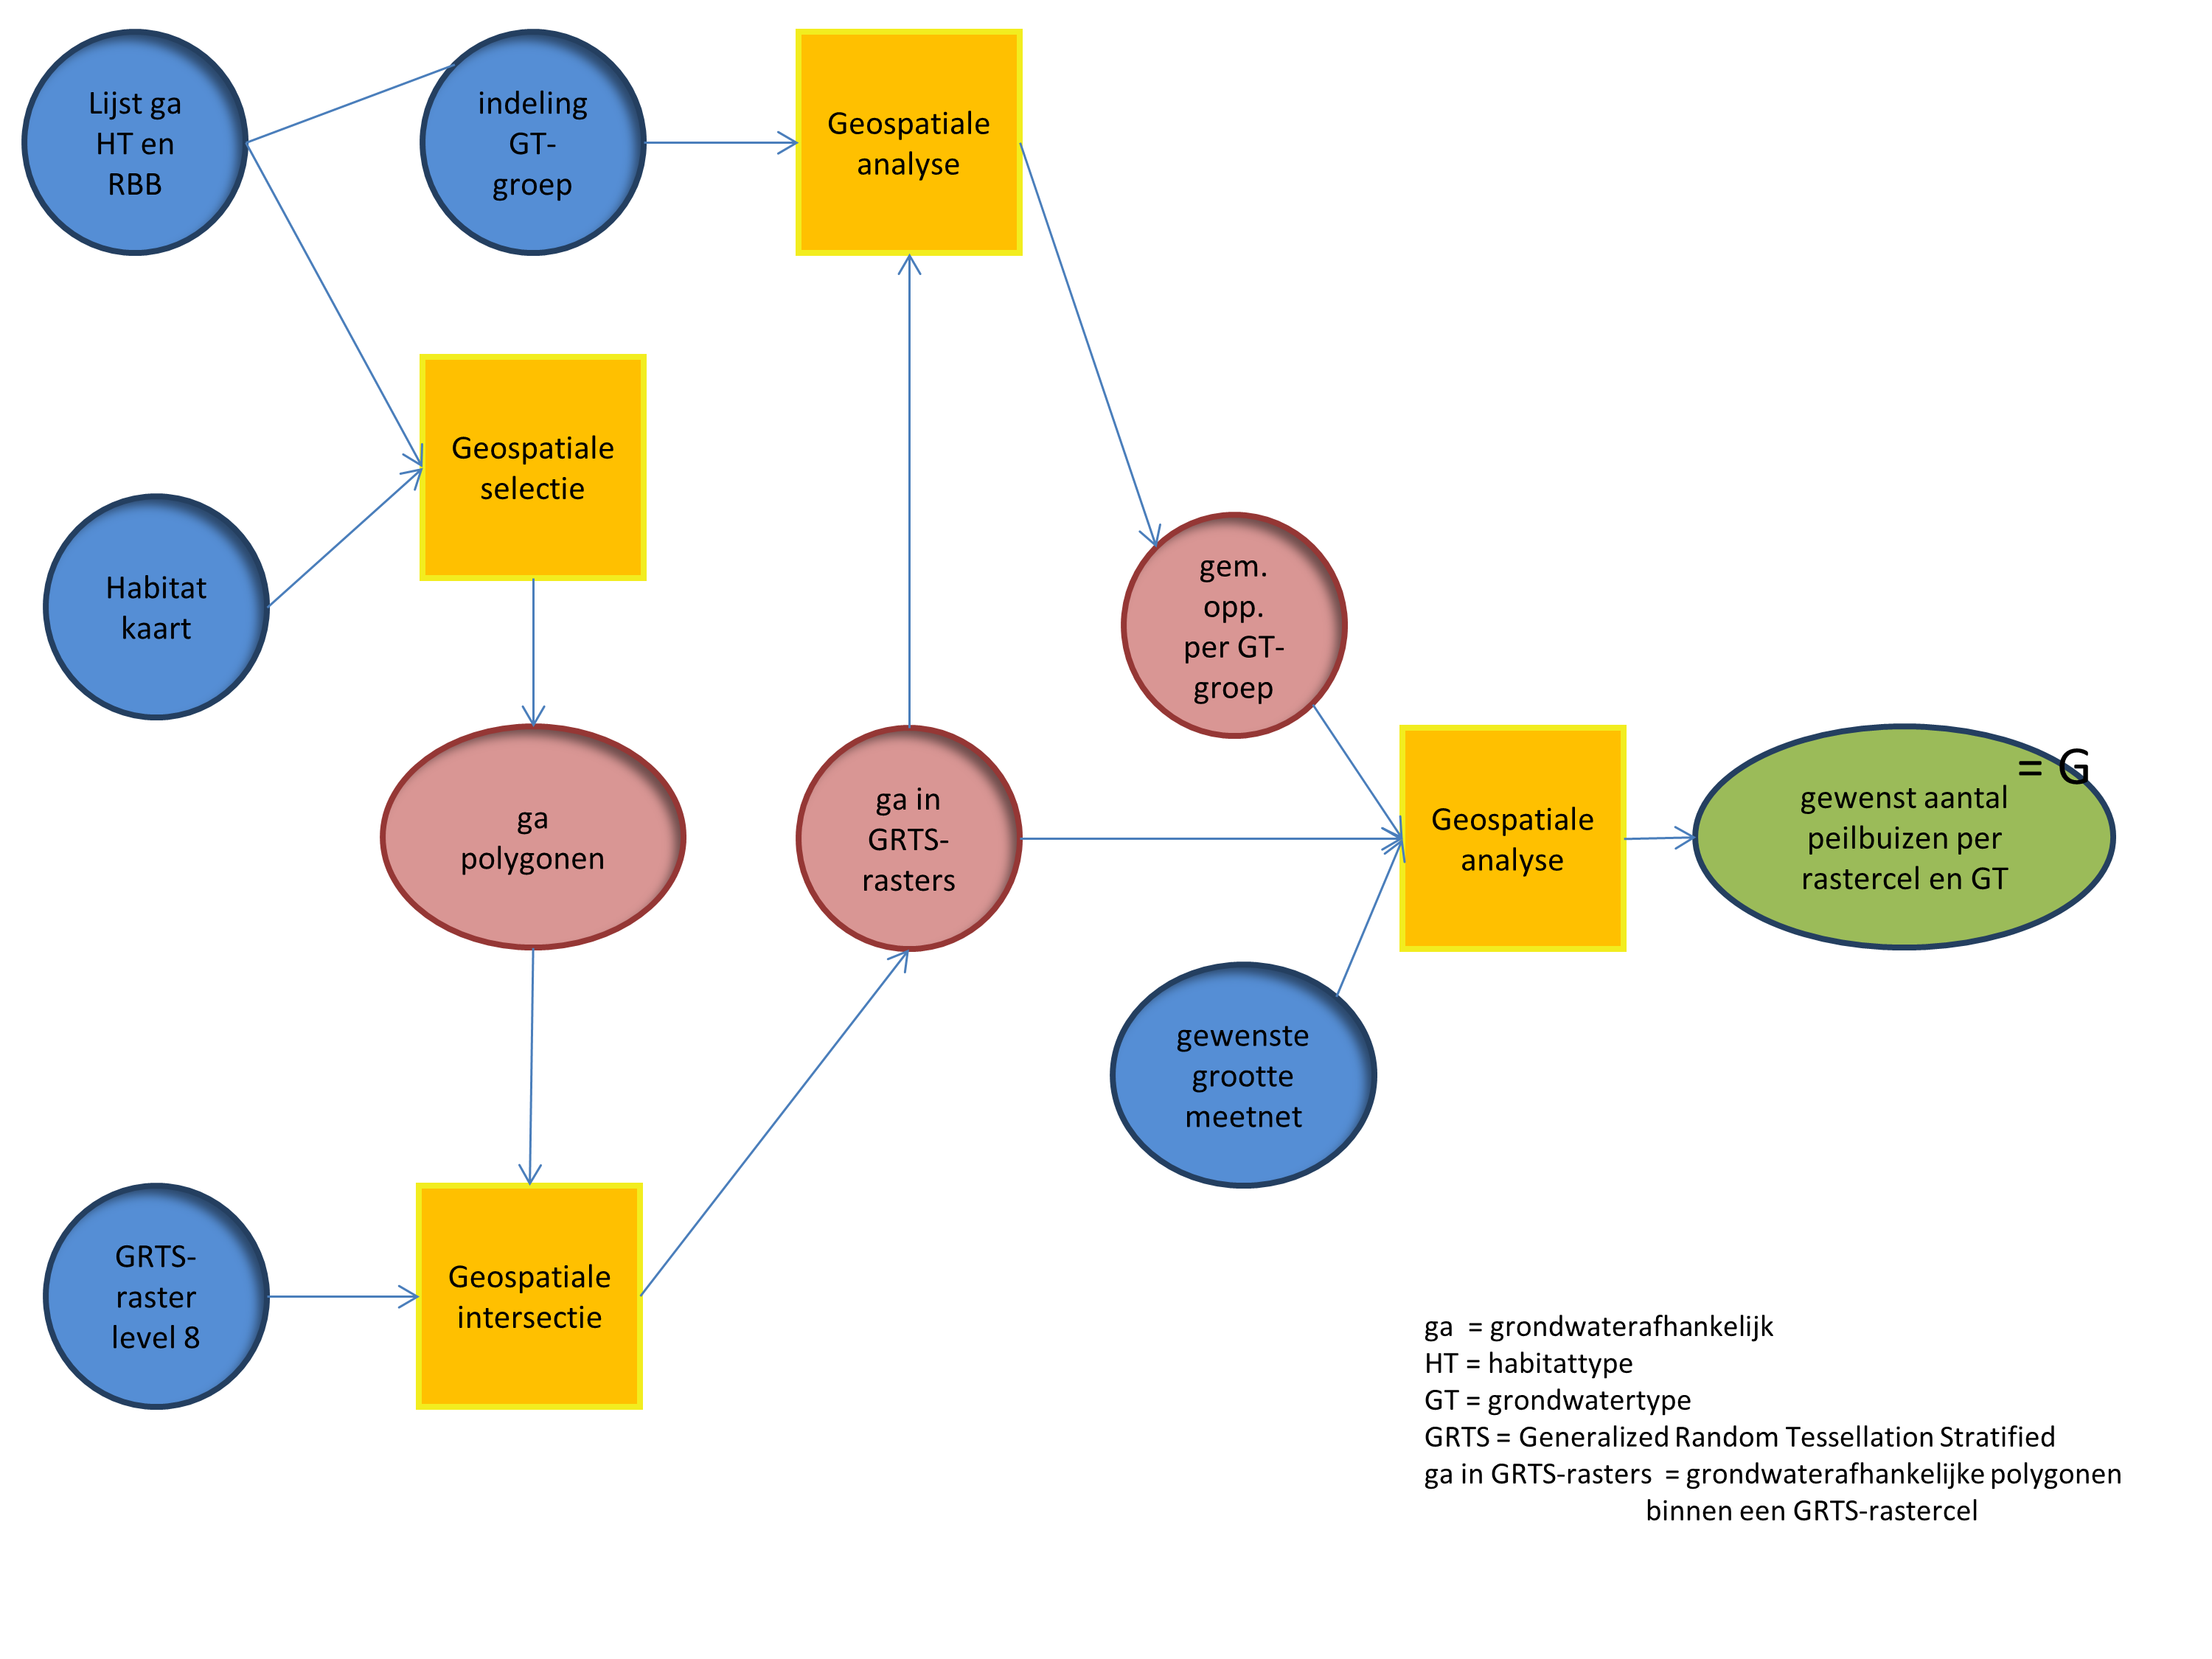
\includegraphics[width=10in]{figures/workflow_rasterselectie} \caption{werkgang selectie rastercellen. Blauw
gekleurde cirkels zijn brongegevens. De rode gekleurde zijn genereerde
data. Het groen gekleurde is een (tussentijds) output-resultaat. De gele
vakken stellen handelingen/bewerkingen voor.}\label{fig:workflow-rastercellen}
\end{figure}

\subsection{Selectie van de
meetpunten}\label{selectie-van-de-meetpunten}

In dit deel bespreken we hoe we aan de gekozen rastercellen effectief
meetpunten kunnen koppelen. Een meetpunt is een locatie waar het
(freatisch) grondwaterpeil periodiek gemeten wordt (of zal worden). In
de praktijk gebeurt dat in een piëzometer of peilbuis.\footnote{Normaal
  gesproken duidt in dit rapport de term meetpunt op de locatie eerder
  dan op het meetinstrument (peilbuis of piëzometer), maar soms slaat
  het op beide. Met peilbuis wordt in dit document ook een piëzometer
  bedoeld.}

Elke locatie die tot één van de GT-groepen behoort, kan in principe in
het meetnet opgenomen worden. Locaties waarvan het onduidelijk is tot
welke GT-groep ze behoren worden niet meegenomen. Dit kunnen locaties
zijn die op grens liggen van habitatvlekken die tot een verschillende
GT-groep behoren of het zijn locaties die in een habitatvlek gelegen
zijn dat gekarteerd is als een complex van vegetaties die tot
verschillende GT-groepen behoren. In de praktijk wordt deze voorwaarde
toegepast door enkel die habitatvlekken en/of peilbuizen te selecteren
die voor 50\% of meer toegewezen kunnen worden aan eenzelfde GT-groep en
die op minstens 3 m afstand liggen van een andere GT-groep.

Figuur \ref{fig:workflow-selectiepb-part1} geeft een schematisch
overzicht van de werkgang die gevolgd werd om na te gaan welke
peilbuizen beschikbaar zijn.




\begin{figure}
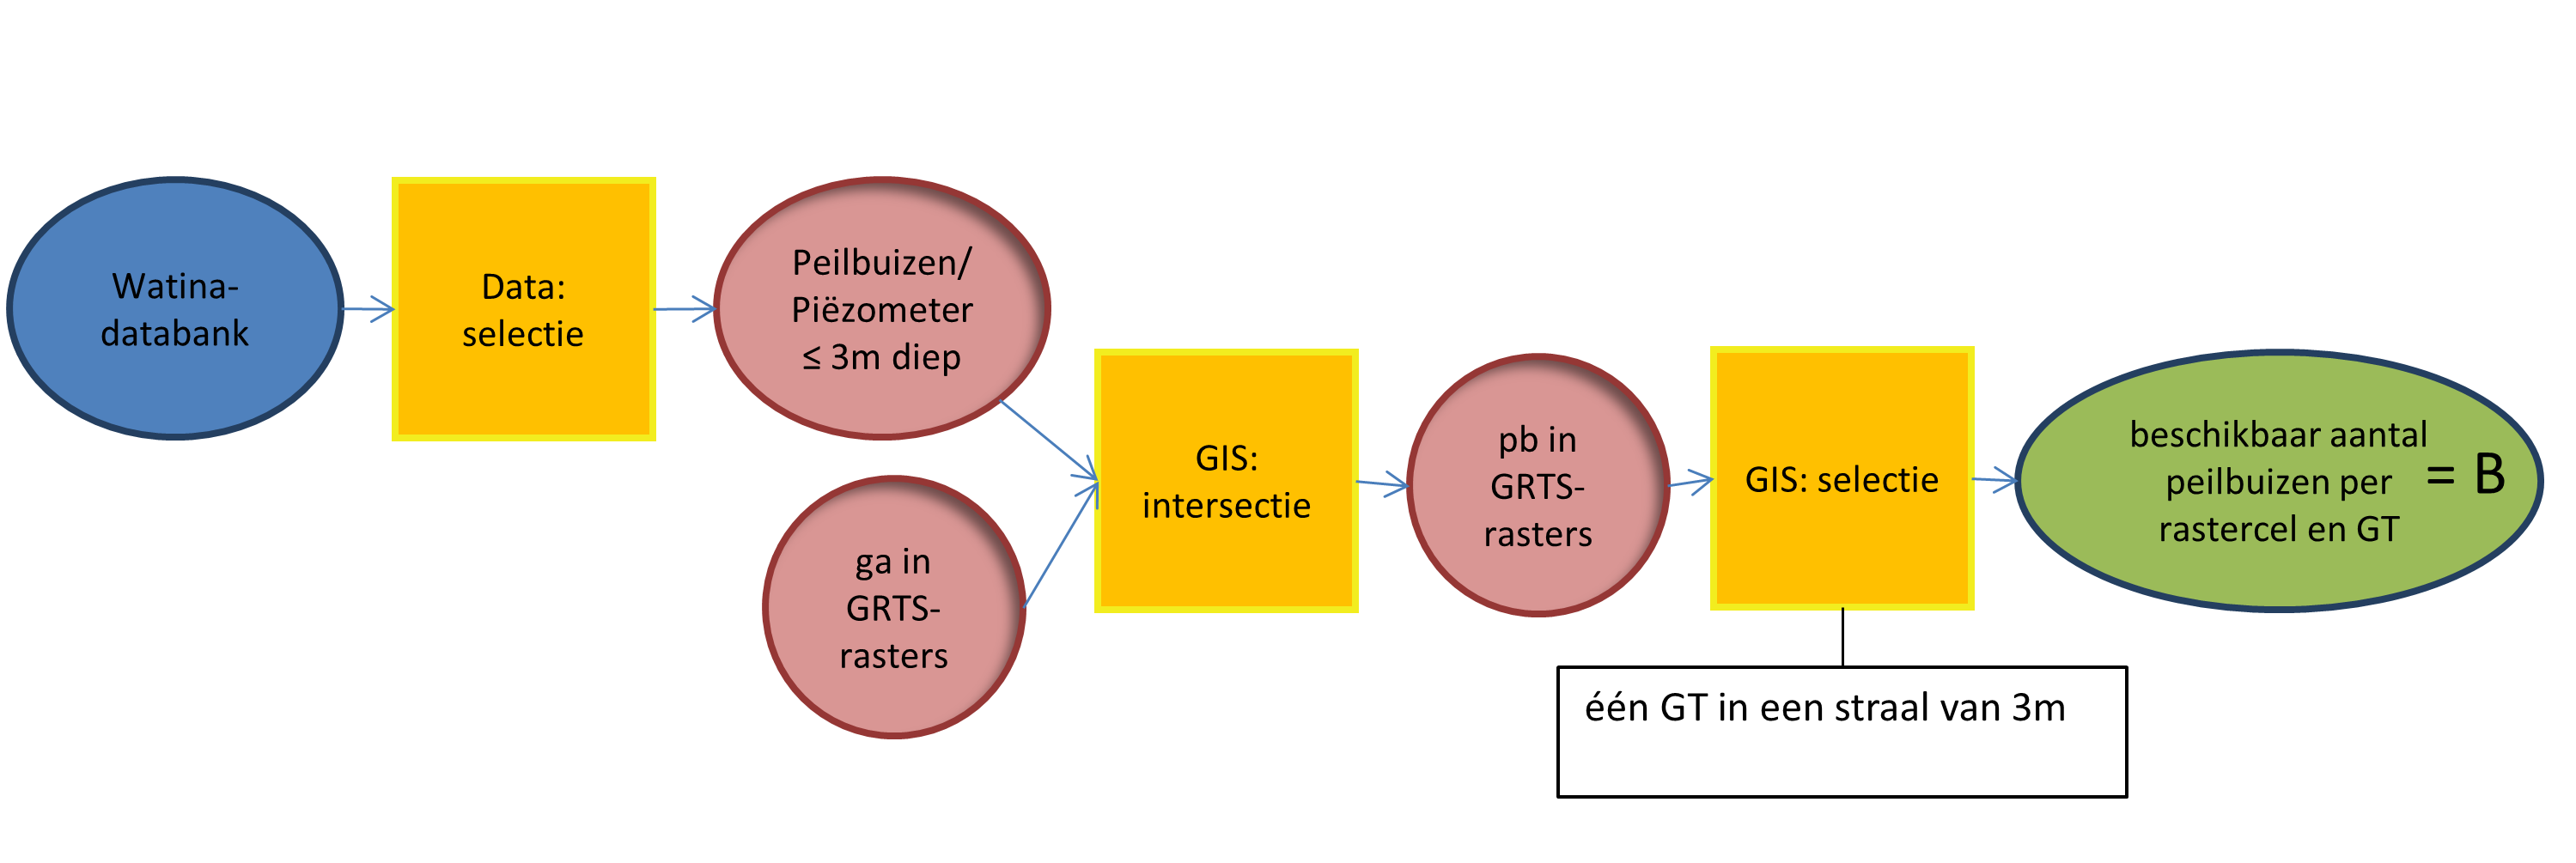
\includegraphics[width=10in]{figures/workflow_pbselectie_part1} \caption{werkgang selectie rastercellen. Voor de
betekenis van de symbolen zie figuur \ref{fig:workflow-rastercellen}.}\label{fig:workflow-selectiepb-part1}
\end{figure}

\subsubsection{Indeling van rastercellen in
categorieën}\label{indeling-cat}

We willen de toewijzing van een meetpunt aan een rastercel afhankelijk
stellen van de verhouding tussen het aantal meetpunten dat voor een
rastercel gezocht wordt (zie hoger) en het aantal effectief beschikbare
meetpunten met een peilbuis.

We willen er ook rekening mee houden dat een beschikbaar meetpunt niet
noodzakelijk ook een geschikt meetpunt is.

Afhankelijk van die verhoudingen worden de \emph{rastercellen}
\textbf{per GT-groep} eerst in categorieën ingedeeld. Deze opdeling is
een hulp bij het ontwerp, omdat elke categorie een specifieke
behandeling vraagt.

\emph{A. Alle meetpunten met een peilbuis zijn kwalitatief
gelijkwaardig}

We stellen eerst voor de eenvoud dat alle beschikbare meetpunten even
geschikt zijn: er wordt bvb. geen onderscheid gemaakt tussen een lang en
een kort bemeten meetpunt. Vergelijken we dan de vraag, het gewenste
aantal meetpunten per rastercel (= G), met het aanbod van meetpunten met
een peilbuis (of kortweg het aantal peilBuizen = B) dan kunnen de
rastercellen in drie categorieën verdeeld worden. De categorieën sluiten
elkaar mutueel uit.

\begin{itemize}
\tightlist
\item
  Cat. 1: de vraag is groter dan het aanbod (G \textgreater{} B)
\end{itemize}

Er zijn geen meetpunten met een peilbuis of er is een gebrek aan.

\begin{itemize}
\tightlist
\item
  Cat. 2: de vraag is gelijk aan het aanbod (G = B)
\end{itemize}

Het aantal beschikbare meetpunten met een peilbuis stemt juist overeen
met het aantal dat gezocht wordt.

\begin{itemize}
\tightlist
\item
  Cat. 3: de vraag is kleiner dan het aanbod (G \textless{} B)
\end{itemize}

Er is een overschot aan meetpunten met een peilbuis.

\textbf{Categorie 1}

Vanuit het oogpunt van een meetnetontwerp kan een rastercel van
categorie 1 over twee soorten meetpunten beschikken. Je hebt meetpunten
zonder peilbuis en mogelijk ook meetpunten met een peilbuis. Specifiek
voor deze categorie is dat we op zoek willen gaan naar nieuwe
meetpunten. Voor de uitwerking van deze selectie van potentiële
geschikte habitatvlekken: zie paragraaf \ref{sel-pot-habvlek}.

Alle meetpunten die reeds een peilbuis hebben, worden zonder verdere
analyse geselecteerd.

\emph{\textbf{Bovenstaande is een voorstel. Je zou ook kunnen beslissen
dat enkel meetpunten met een peilbuis in aanmerking komen voor het
meetnet.}} \emph{\textbf{Of het tegenovergestelde is ook een
alternatief: dat voor de ruimtelijke balancering we geen voorkeur geven
aan meetpunten met een peilbuis en enkel rekening houden met het
voorkomen van geschikte (ttz behoren tot de gewenste GT-groep)
habitatvlekken.}} \emph{\textbf{We vinden dat het huidige voorstel een
goede balans vertoont tussen beide.}}

Het gaat hier vooral over een tijdsinvestering: dergelijke meetpunten
zullen pas na enkele jaren effectief kunnen meedraaien in het meetnet.
In afwachting daarvan zal het meetnet dus met een kleiner aantal
meetpunten moeten functioneren.

\textbf{Categorie 2}

De rastercellen van deze categorie zijn voor het meetnetontwerp een
zegen. Het aantal locaties met peilbuizen volstaat juist om te voldoen
aan de vraag. Alle locaties kunnen zonder verdere analyse in het meetnet
worden opgenomen.

\textbf{Categorie 3}

Voor een rastercel van categorie 3 stelt er zich een `luxe-probleem': er
is namelijk een overschot aan meetpunten met een peilbuis. Uit dit
aanbod moet nog het gewenste aantal meetpunten gekozen worden. Hiervoor
verwijzen we naar paragraaf \ref{sel-habvlek}.

\emph{B. De meetpunten met een peilbuis zijn kwalitatief niet
gelijkwaardig}

In werkelijkheid zijn niet alle meetpunten even geschikt.

De bovenstaande categorie-indeling blijft weliswaar behouden, maar er
zijn verschillen t.a.v. de selectie van meetpunten en het gebruik ervan
in het meetnet.

We noemen een meetpunt geschikt, indien er hiervoor een
droogte-indicator kan berekend worden. Het berekenen van deze indicator
op een meetpunt vergt een ononderbroken meetreeks van \emph{dagelijkse}
peilen en dit over een stabiele, langdurige periode (een paar tiental
jaren) . De beschikbare terreinwaarnemingen in Watina zijn hiervoor
meestal ontoereikend. Door middel van een tijdreeksanalyse (zie
\ref{tijdreeksanalyse}) kunnen de tijdreeksen met modelgegevens
aangevuld worden, waardoor het wel mogelijk wordt om de indicator te
berekenen.

Het zal bijgevolg op basis van de tijdreeksanalyse zijn dat meetpunten
als geschikt (een tijdsmodel is mogelijk) of niet geschikt (een
tijdsmodel is niet mogelijk) zullen bevonden worden. Deze evaluatie
willen we vertalen in het gebruik van het meetpunt in het meetnet. Een
geschikt meetpunt kan op basis van de data onmiddellijk in het meetnet
worden opgenomen. Een niet geschikt meetpunt daarentegen kan dat pas na
verloop van tijd, nl. wanneer er voldoende data zijn die toelaten een
betrouwbaar tijdreeksmodel (zie onder) te bouwen.

Het vergt veel tijd om op alle beschikbare meetpunten een
tijdreeksanalyse uit te voeren. We willen dit beperken tot de
\emph{relatief (beschouwd op het niveau van combinatie rastercel en
GT-groep)} kwalitatief beste meetreeksen. Dit is een selectie, maar we
leggen geen absolute minimum-criteria op. Dit wil zeggen dat indien
bijvoorbeeld in een rastercel voor een bepaalde GT-groep de langste
tijdreeks één jaar is, dan zal deze peilbuis toch voor een
tijdreeksanalyse geselecteerd kunnen worden. De kans wordt uiteraard
kleiner dat met deze beperkte data een betrouwbaar model kan gebouwd
worden.

We delen de meetpunten daarom op in een aantal kwaliteitsklassen op
basis van volgende
\textbf{\protect\hypertarget{basiskwaliteitscriteria}{}{basiskwaliteitscriteria}}
:

\begin{enumerate}
\def\labelenumi{(\arabic{enumi})}
\item
  De meetpunten hebben vanaf 2000 voor minstens één jaar een goede
  tijdreeks\footnote{Een kwalitatief goed meetjaar wordt hier
    gedefinieerd als een hydrologisch jaar waarvoor een lg3 kan berekend
    worden. Dit houdt in dat er minstens 20 goed gespreide metingen per
    jaar zijn. Het verschil tussen twee metingen mag niet groter zijn
    dan 30 dagen en de eerste en laatste meting moet resp. in april en
    maart (van het daaropvolgende kalenderjaar) vallen. lg3 = het
    gemiddelde van de drie laagste waterpeilen binnen een hydrologisch
    jaar (1 april - 31 maart), waarbij er tussen deze drie metingen
    minstens 14 dagen verschil ligt. --\textgreater{}}, die een toelaat
  een zogenaamde lg3-waarde\footnote{Een kwalitatief goed meetjaar wordt
    hier gedefinieerd als een hydrologisch jaar waarvoor een lg3 kan
    berekend worden. Dit houdt in dat er minstens 20 goed gespreide
    metingen per jaar zijn. Het verschil tussen twee metingen mag niet
    groter zijn dan 30 dagen en de eerste en laatste meting moet resp.
    in april en maart (van het daaropvolgende kalenderjaar) vallen. lg3
    = het gemiddelde van de drie laagste waterpeilen binnen een
    hydrologisch jaar (1 april - 31 maart), waarbij er tussen deze drie
    metingen minstens 14 dagen verschil ligt. --\textgreater{}} te
  berekenen.
\item
  Meetpunten met een \emph{recente} kwalitatief goede tijdreeks primeren
  boven meetpunten met een oudere tijdreeks.
\end{enumerate}

De meetpunten worden hierbij gerangschikt volgens aflopend jaartal
(eindjaar) van de laatst beschikbare kwalitatief goede tijdreeks.

Meetpunten worden als evenwaardig beschouwd als het verschil niet groter
dan \textbf{5} jaar is.

\begin{enumerate}
\def\labelenumi{(\arabic{enumi})}
\setcounter{enumi}{2}
\tightlist
\item
  Meetpunten met een \emph{langere} tijdreeks, t.t.z. een groter aantal
  kwalitatief goede meetjaren, krijgen ook een hogere prioriteit.
\end{enumerate}

Meetpunten waarvan het aantal niet meer dan \textbf{5} jaar van elkaar
verschilt, worden als evenwaardig beschouwd.

\begin{enumerate}
\def\labelenumi{(\arabic{enumi})}
\setcounter{enumi}{3}
\tightlist
\item
  Een meetpunt met een lange tijdreeks, maar niet recent, primeert op
  een meetpunt met een recentere maar
  \protect\hypertarget{derde-criterium}{}{kortere tijdreeks.}
\end{enumerate}

Deze basiskwaliteitscriteria zijn te beschouwen als een eerste screening
op basis van actueel beschikbare feitelijke grondwatermetingen.

Het gebruik van deze criteria leidt er ook toe dat in een rastercel bij
de toewijzing van een meetpunt, indien mogelijk (= in categorie 3),
rekening wordt gehouden met de datakwaliteit.

\textbf{\emph{vraag: wat te doen met bestaande meetlocaties die actueel
niet geschikt zijn? Worden deze weer geactiveerd (gevolgd in deze
versie) of geven we voorrang aan de ruimtelijke balans ?}}

\subsubsection{Tijdreeksanalyse}\label{tijdreeksanalyse}

Tijdreeksanalyse is een middel om grondwaterstandsmetingen te analyseren
(zie bijv. Von Asmuth \emph{et al.},
\protect\hyperlink{ref-RN877}{2004}). In feite zouden ook meetreeksen
van oppervlaktewaterpeilen geanalyseerd kunnen worden, maar dit is
weinig gebruikelijk, waarschijnlijk omdat er moeilijker een verband te
leggen is met het weer (zoals neerslag en verdamping). In dit project
willen we deze analysetechniek toepassen op grondwatermeetreeksen met
twee doeleinden:

\begin{itemize}
\tightlist
\item
  het verlengen of invullen van te korte of onregelmatige
  grondwaterstandsreeksen
\item
  het opsporen van lineaire trends
\end{itemize}

Het eerste doel is ook al hoger ter sprake gekomen. Slagen we er in om
op een betrouwbare wijze de waterstandsreeksen te
verlengen/vervolledigen, dan kan een meetpunt geschikt worden om in het
droogtemeetnet opgenomen te worden. De tijdreeksen krijgen ook een meer
uniforme lengte, waardoor het afleiden van een droogte-indicator meer
gestandaardiseerd wordt.

Het tweede doel is in feite een bijkomende selectiecriterium. Indien uit
een tijdreeksanalyse blijkt dat de waterstanden van een meetpunt
systematisch dalen of stijgen, leent dat meetpunt zich niet goed voor
het berekenen van een droogte-indicator. Met een systematische daling of
stijging bedoelen we een lineaire trend die niet door externe factoren
(opstuwen of graven greppels, waterwinning) kan verklaard worden. Indien
een tijdreeks een lineaire trend vertoont, wordt het meetpunt als
momenteel ongeschikt beschouwd.

Voor de tijdreeksanalyse doen we beroep op het computerprogramma
Menyanthes (KWR \& Waterware, \protect\hyperlink{ref-RN5899}{2018}).
Voor het samenstellen van de verklarende reeksen (neerslag en
evapotranspiratie) werd beroep gedaan op de data van de meetstations
beheerd door KMI, VMM, HIC en KNMI. Voor de waterstandgegevens werd de
Watina-databank geraadpleegd.

Er werden, zoals hoger al aangehaald, geen kwaliteitseisen gesteld aan
een meetreeks die deze a priori zou uitsluiten van een tijdreeksanalyse.
Het is, door het hoge aantal beschikbare meetpunten, echter niet
doenbaar om een tijdreeksanalyse uit te voeren op alle meetpunten.

Wel werden alle meetreeksen van de meetpunten die behoren tot
rastercellen van cat. 1 en cat. 2 geanalyseerd. Voor categorie 3 bleef
dat beperkt tot die meetpunten die behoren tot de hoogste
kwaliteitsklassen die nodig zijn om tot het gewenst aantal meetpunten te
komen.

Een meetreeks werd weerhouden als er een tijdsmodel kon voor
samengesteld worden dat minstens 66\% van de variatie in de waargenomen
peilen (cfr. EVP, explained variance percentage, in de
Menyanthes-software) kon verklaren en ook geen significante lineaire
trend vertoont. Bij het tijdsmodel werden uitsluitend neerslag- en
evapotranspiratiedata als verklarende reeksen gebruikt.

Minstens twee derden van het peilverloop dient dus verklaard te kunnen
worden door het weer. Eén derde kan/mag door andere factoren beïnvloed
worden (bijv. het naburige peil van een waterloop).

Een \protect\hypertarget{lintrend}{}{lineaire trend} werd als
significant beschouwd indien de stijging/daling per jaar (=
\texttt{trend}), rekening houdend met de standaardafwijking hierop (=
\texttt{se}), voldoet één van de volgende twee regels:

\[trend - 1.96* se > 1(cm/jaar)\] of \[trend + 1.96* se < -1(cm/jaar)\]
Er is dan 2.5\% kans een trendwaarde die groter resp. kleiner is ten
onrechte als een significante trend te bestempelen.

De kwaliteit van een tijdreeks kan na een tijdreeksanalyse anders
beoordeeld worden. Bijvoorbeeld een meetpunt met veel peilmetingen, die
echter een duidelijke lineaire trend vertonen, is weinig geschikt om
onmiddellijk in het meetnet te worden opgenomen. Anderzijds komt een
meetpunt met minder metingen, maar waarvoor een goed model kan gebouwd
worden (zonder lineaire trend), wel in aanmerking om nu reeds in het
meetnet te worden opgenomen.

Bij de modelselectie kwam toch ook nog expertoordeel bij kijken.

De gestelde kwaliteitseisen leiden niet tot uitsluiting van een
tijdreeksanalyse. In principe kan elke peilbuis, zelfs al is er maar één
meting van bekend, geselecteerd worden. En zo geschiedde ook. Deze
meetreeksen werden manueel afgekeurd. Sommige heel korte tijdreeksen
hadden zelfs bijna een perfecte fit, maar het was toch onbetrouwbaar om
hiermee waarden te simuleren over een relatief lange tijdsperiode.

Anderzijds werd een model met een verklarende variantie beneden 66\%
soms nog weerhouden, indien bleek dat het model de lage
grondwaterstanden goed kon modelleren.

Een lange tijdreeks met een trend \textless{} 1cm/jaar, maar waarbij de
peilen maar weinig schommelen (kleine amplitude) kon toch owv deze trend
afgekeurd worden (bijv. een tijdreeks waarbij over 15 jaar er een
duidelijke stijging van 10 cm te zien is, terwijl de peilen slechts een
amplitude van 40 cm hebben) en vice versa.

Het al dan niet weerhouden van een tijdreeks kan in categorie 3 gevolgen
hebben voor het selecteren van een meetpunt. Immers hierbinnen wordt
gestreefd minstens zoveel geschikte meetpunten te vinden dan er gezocht
worden. Zijn er meer geschikte punten dan gezocht, dan kan gestopt
worden met verder zoeken. Zolang dit aantal echter niet bereikt is,
wordt (iteratief) verder gezocht.

\subsubsection{Bijkomende GRTS-analysen}\label{bijkomende-grts-analysen}

Afhankelijk van de verhouding tussen het aantal gewenste, beschikbare
enerzijds (categorie 1) en het aantal gewenste en geschikte peilbuizen
anderzijds (categorie 3), moeten er nog enkele bijkomende GRTS-analysen
uitgevoerd worden.

\paragraph{Selecteren van potentiële geschikte habitatvlekken voor
rastercellen waarvoor er te weinig peilbuizen bestaan (cat.
1)}\label{sel-pot-habvlek}

Voor rastercellen van cat. 1 is er een nood aan één of meer extra
meetpunten. Om hierbinnen (8192 * 8192 m) de plaatskeuze zo aselect
mogelijk te doen, doen we beroep op het fijnste GRTS-raster
`GRTSmaster\_habitats' (celgrootte = 32 m). Opnieuw wordt op deze manier
een synergie bekomen met de aselecte locatiekeuzes in MNM. Elk
deelrastercel heeft binnen de rastercel een bepaalde rangnummer. Alleen
deelrastercellen \emph{die voor het merendeel vegetaties bevatten die
tot de GT-groep behoren} komen voor selectie in aanmerking. De
deelrastercel(len) met het /de laagste rangnummer(s) zal/zullen dan
geselecteerd worden. Aan de selectie van deelrastercellen kunnen, naast
de aanwezigheid van de juiste GT-groep, nog bijkomende voorwaarden
gekoppeld worden (beheerder, \ldots{}). Blijkt bij inspectie op terrein
dat de geselecteerde plaats toch niet aan de verwachtingen/criteria
voldoet, dan wordt binnen dezelfde rastercel de rastercel die het eerst
in rang volgt binnen een zoekstraal van 1 km bezocht.

\paragraph{Selecteren van een meetpunt in een rastercel waarvoor
meerdere kandidaten zijn (cat. 3)}\label{sel-habvlek}

Afhankelijk van de verhouding tussen gewenste aantal en het aantal
geschikte peilbuizen is er mogelijk een extra analyse nodig.

\begin{itemize}
\item
  Is het aantal geschikte peilbuizen groter dan wordt enkel binnen deze
  groep een GRTS-analyse uitgevoerd om het gewenste aantal te
  selecteren.
\item
  Is het aantal kleiner dan wordt er uit alle beschikbare peilbuizen via
  een GRTS-analyse het gewenste aantal geselecteerd.
\item
  Is het aantal gelijk dan hoeft er geen verdere analyse te gebeuren.
  Alle meetpunten kunnen in het meetnet worden opgenomen.
\end{itemize}

Net zoals voor cat. 1 willen we de keuze zo aselect mogelijk doen. We
doen hiervoor terug beroep op het fijnste GRTS-raster
`GRTSmaster\_habitats' (celgrootte = 32 m). Het/de meetpunt(en) gelegen
in de deelrastercel(len) met het /de laagste rangnummer(s) zal/zullen
dan geselecteerd worden. Deze werkwijze laat ook gemakkelijk toe om
reserve-punten te kiezen. Het zijn de meetpunten die in rang volgen op
de laagste rang van een gekozen punt.

\subsubsection{Samenvatting werkgang selectie
peilbuizen}\label{samenvatting-werkgang-selectie-peilbuizen}

Na de ruimtelijke selectie weten we hoeveel meetpunten er per rastercel
en per GT-groep gewenst zijn.

We proberen die wensen zoveel mogelijk in te vullen met bestaande
peilbuizen waarvan hun meetreeksen toelaten een droogte-indicator te
berekenen.

Hiertoe evalueren we de kwaliteit van de meetreeksen op basis van de
mogelijkheid om voor minstens één jaar een lg3 te berekenen voor de
metingen na 2000, van het aantal meetjaren en van de ouderdom van de
meetreeks.

De kwalitatief beste meetreeksen worden verder beoordeeld met een
tijdreeksanalyse. Door het grote aantal peilbuizen was het niet mogelijk
ze alle te analyseren. De voorkeur ging daarom uit naar de relatief
beste reeksen. Een meetreeks wordt `geschikt' bevonden als minstens 2/3
van de variatie door het weer kan verklaard worden en er in de reeks
geen lineaire trend te zien is. Op basis van de tijdreeksanalyse worden
de meetreeksen geherklasseerd in `geschikt', `niet 'geschikt' en
`onbekend' (indien niet behandeld). Er worden minstens zoveel peilbuizen
geanalyseerd tot er evenveel of meer geschikte reeksen zijn dan het
gewenste aantal, zoniet worden ze allemaal geanalyseerd.

Is een meetreeks `geschikt', dan kan de peilbuis onmiddellijk in het
meetnet opgenomen worden. Is ze `niet geschikt', dan kan dit pas na
verloop van enkele jaren.

De rastercellen kunnen in drie categorieën (cat. 1- 3) verdeeld worden
op basis van de verhouding tussen het aantal gewenste en beschikbare
peilbuizen. Bij cat. 1 zijn er te weinig peilbuizen. De meetreeksen van
alle peilbuizen werden geanalyseerd. Via een GRTS-procedure wordt het
ontbrekend aantal aangevuld met habitatvlekken. In cat. 2 klopt het
gewenste aantal met het beschikbaar aantal en hoeft er geen aansluitende
analyse meer uitgevoerd te worden.

In cat. 3 zijn er meer peilbuizen beschikbaar. Afhankelijk van de
verhouding tussen het gewenste aantal en het aantal geschikte peilbuizen
is er mogelijk een extra GTRS-analyse nodig om het gewenste aantal te
selecteren.

Figuur \ref{fig:workflow-selectiepb-part2} geeft schematisch het
overzicht van de werkgang die gevolgd werd om uit de beschikbare
peilbuizen meetpunten te selecteren en deze desnoods aan te vullen met
nieuwe.




\begin{figure}
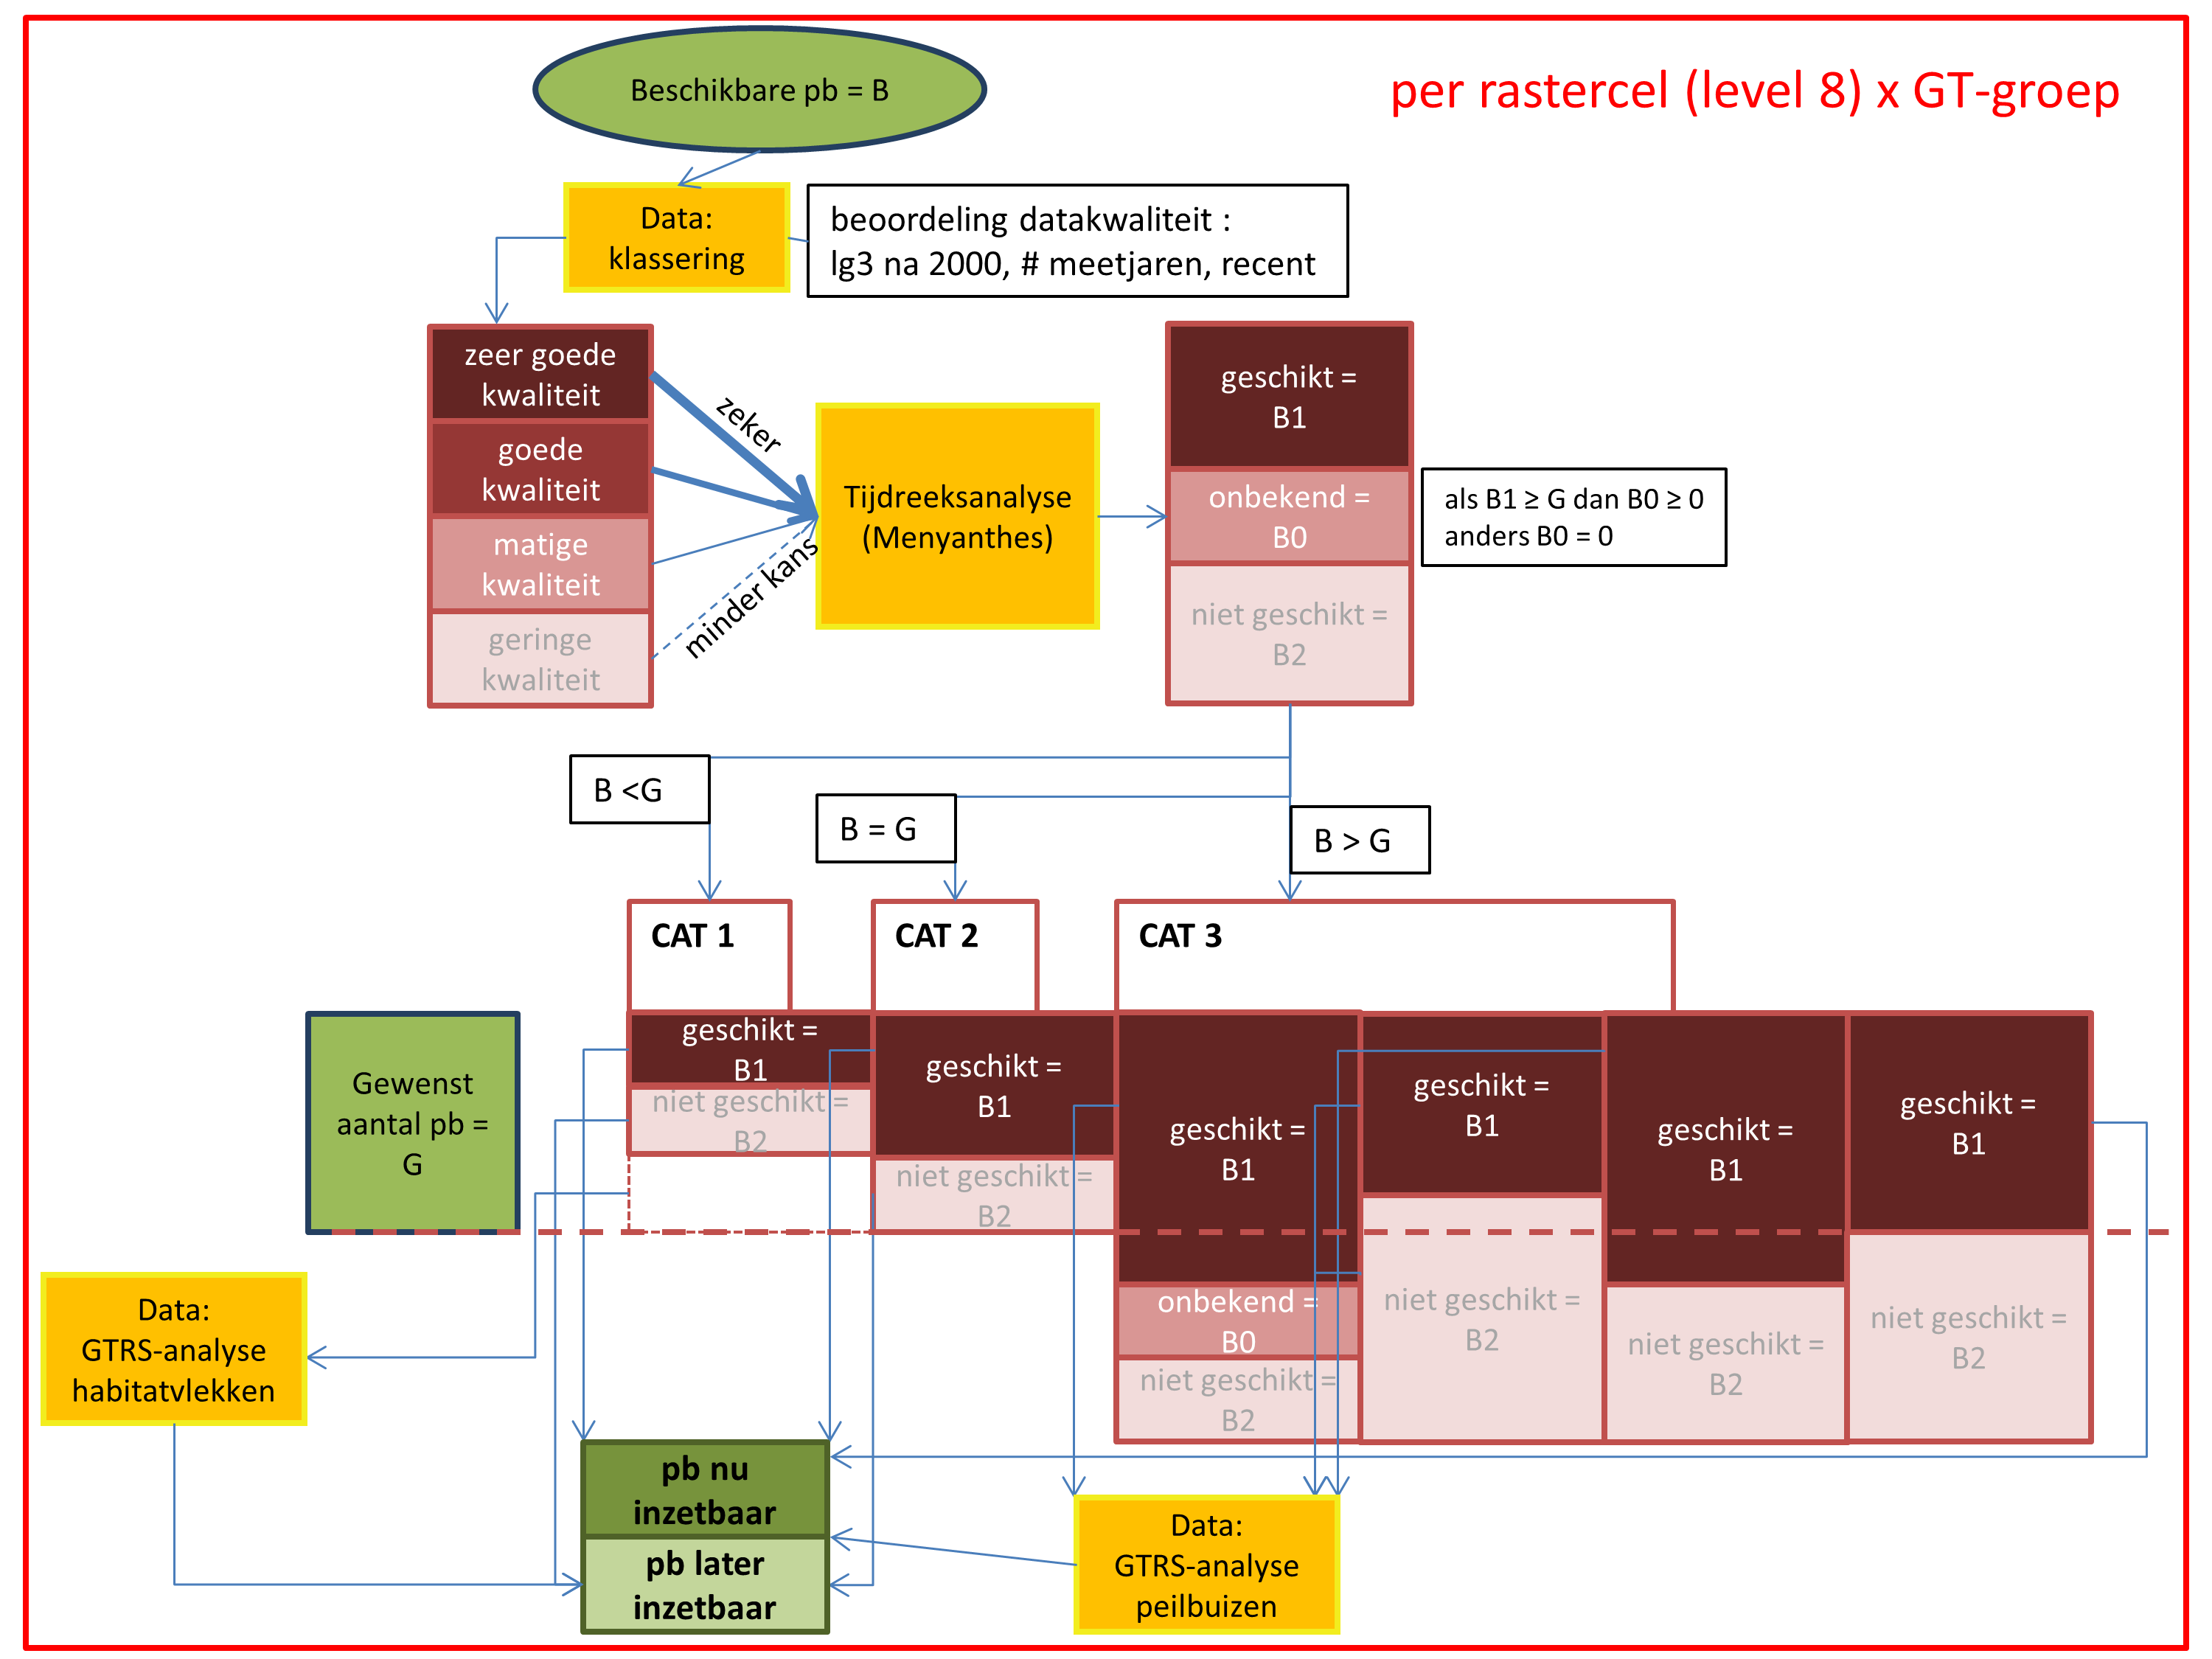
\includegraphics[width=10in]{./figures/workflow_pbselectie_part2} \caption{werkgang selectie rastercellen. Voor de
betekenis van de symbolen zie figuur \ref{fig:workflow-rastercellen}.}\label{fig:workflow-selectiepb-part2}
\end{figure}

\section{Bepaling droogte-indicator voor de geselecteerde
punten}\label{bepaling-droogte-indicator-voor-de-geselecteerde-punten}

\subsection{Droogte-indicatoren}\label{droogte-indicatoren}

Er zijn verschillende indicatoren mogelijk om droogte te detecteren
(Wouters \emph{et al.}, \protect\hyperlink{ref-RN5703}{2018}).

Binnen dit project berekenen we de huidig gebruikte droogte-indicator:
De indicator vergelijkt de grondwaterstand op een gegeven dag met de
grondwaterstanden die op diezelfde plaats en dag van het jaar zijn
voorgekomen in het verleden. De indicator evalueert dus de
droogtetoestand rekening houdend met de tijd van het jaar. Zo kunnen ook
relatief lage grondwaterstanden in het voorjaar als droogte aangeduid
worden.

De indicator kleurt respectievelijk rood, oranje of geel op een bepaalde
plaats en dag zodra de grondwaterstand er minstens 14 dagen onder de
p10, p20 of p30 (situatie met overschrijdingskans van 10, 20 of 30\%) is
gebleven. \emph{\textbf{De indicator kleurt respectievelijk rood, oranje
of geel voor Vlaanderen als minstens de helft van de putten kleurcode
rood, oranje of geel heeft. (vraag: is dit ook aangewezen voor dit
meetnet ?). }} \emph{\textbf{Een opsplitsing per bekken hadden we
tijdens de eerste vergadering niet weerhouden.}}

\subsection{Berekeningswijze voor de geselecteerde
punten}\label{berekeningswijze-voor-de-geselecteerde-punten}

Voor het berekenen van de droogte-indicator doen we beroep op
tijdreeksen van \textbf{\emph{minimaal 20 (of meer?) jaren lang}}, al
dan niet gemodelleerde, metingen en waarbij metingen van 2017 en 2018
uitgesloten werden. Het is namelijk nu nog onduidelijk of de actuele
vegetatie geen nadelige effecten van deze twee droge zomers heeft gekend
(door naijling). Voor elke bestaande geselecteerde meetlocatie wordt dan
voor elke dag van het jaar (\textbf{\emph{vraag: of alleen voor het
groeiseizoen: 1 april - 1 oktober? }}) de p10, p20 en p30
percentielwaarde berekend.

\chapter{Uitvoering}\label{uitvoering}

De toepassing van de hiervoor besproken methodiek is volledig gebeurd
met R versie 3.6.1 (R Core Team
(\protect\hyperlink{ref-citingR}{2019})), tenzij anders vermeld. Meer
details hierover is vermeld in bijlage \ref{gebruikte-werkomgeving}.

De code voor analyse en dit rapport is ook te vinden op de
GitHub-repository
\href{https://github.com/inbo/n2khab-droogtemeetnet}{n2khab-droogtemeetnet}.

\section{Keuze rasterlaag}\label{keuze-rasterlaag}

Voor de ruimtelijk gebalanceerde selectie in functie van de verspreiding
van de gaHT kiezen we een opgeschaalde variant van de Vlaamse
\texttt{GRTSmaster\_habitats} databron, meer bepaald op `level 8'
(\href{https://doi.org/10.5281/zenodo.3354405}{bron}), t.t.z. met cellen
van 8192 m (figuur \ref{fig:meetnetontwerp}).

\begin{figure}
\centering
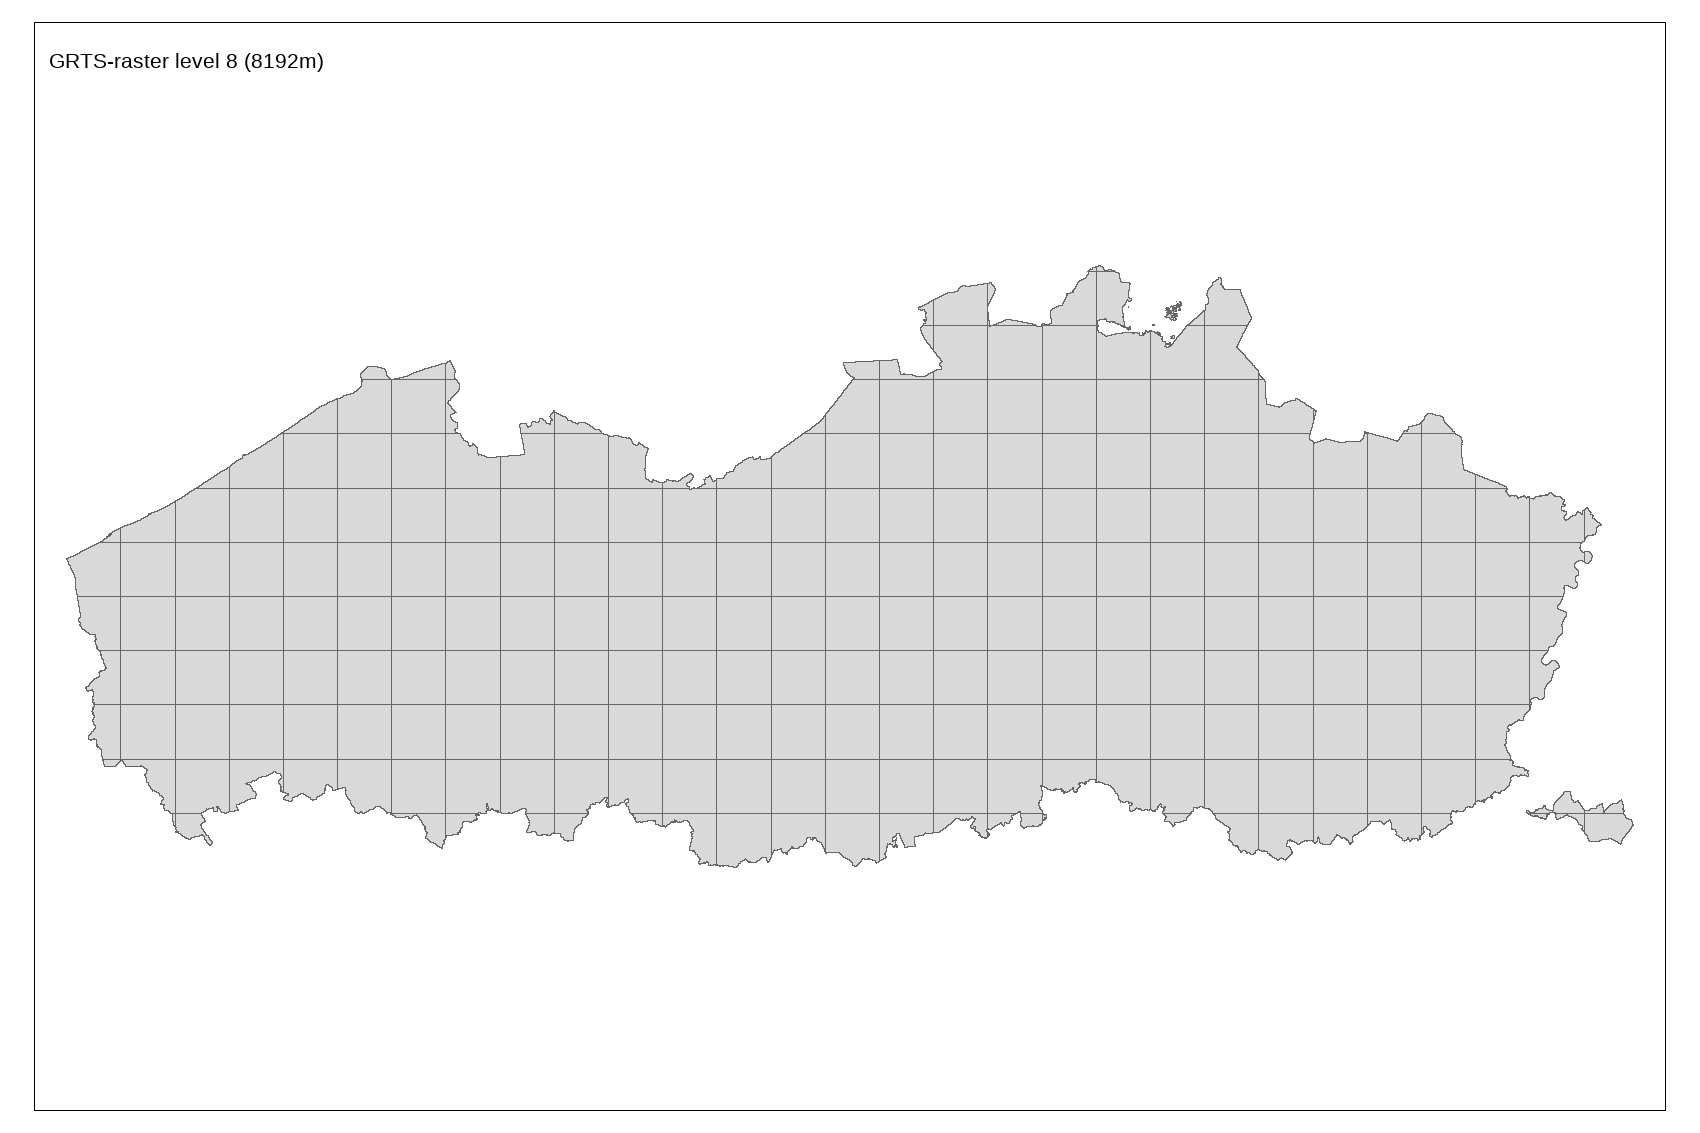
\includegraphics{droogtemeetnet_ontwerp_files/figure-latex/meetnetontwerp-1.pdf}
\caption{\label{fig:meetnetontwerp}Het GRTS-raster voor Vlaanderen, level 8
(8192m)}
\end{figure}

\section{Selectie rastercellen}\label{selectie-rastercellen}

Op basis van deze rasterlaag maken we een overlay met de verspreiding
van de vijf grondwatergroepen volgens de habitatkaart (figuur
\ref{fig:overlay-habitatkaart-GRTS-plot}).

\begin{figure}
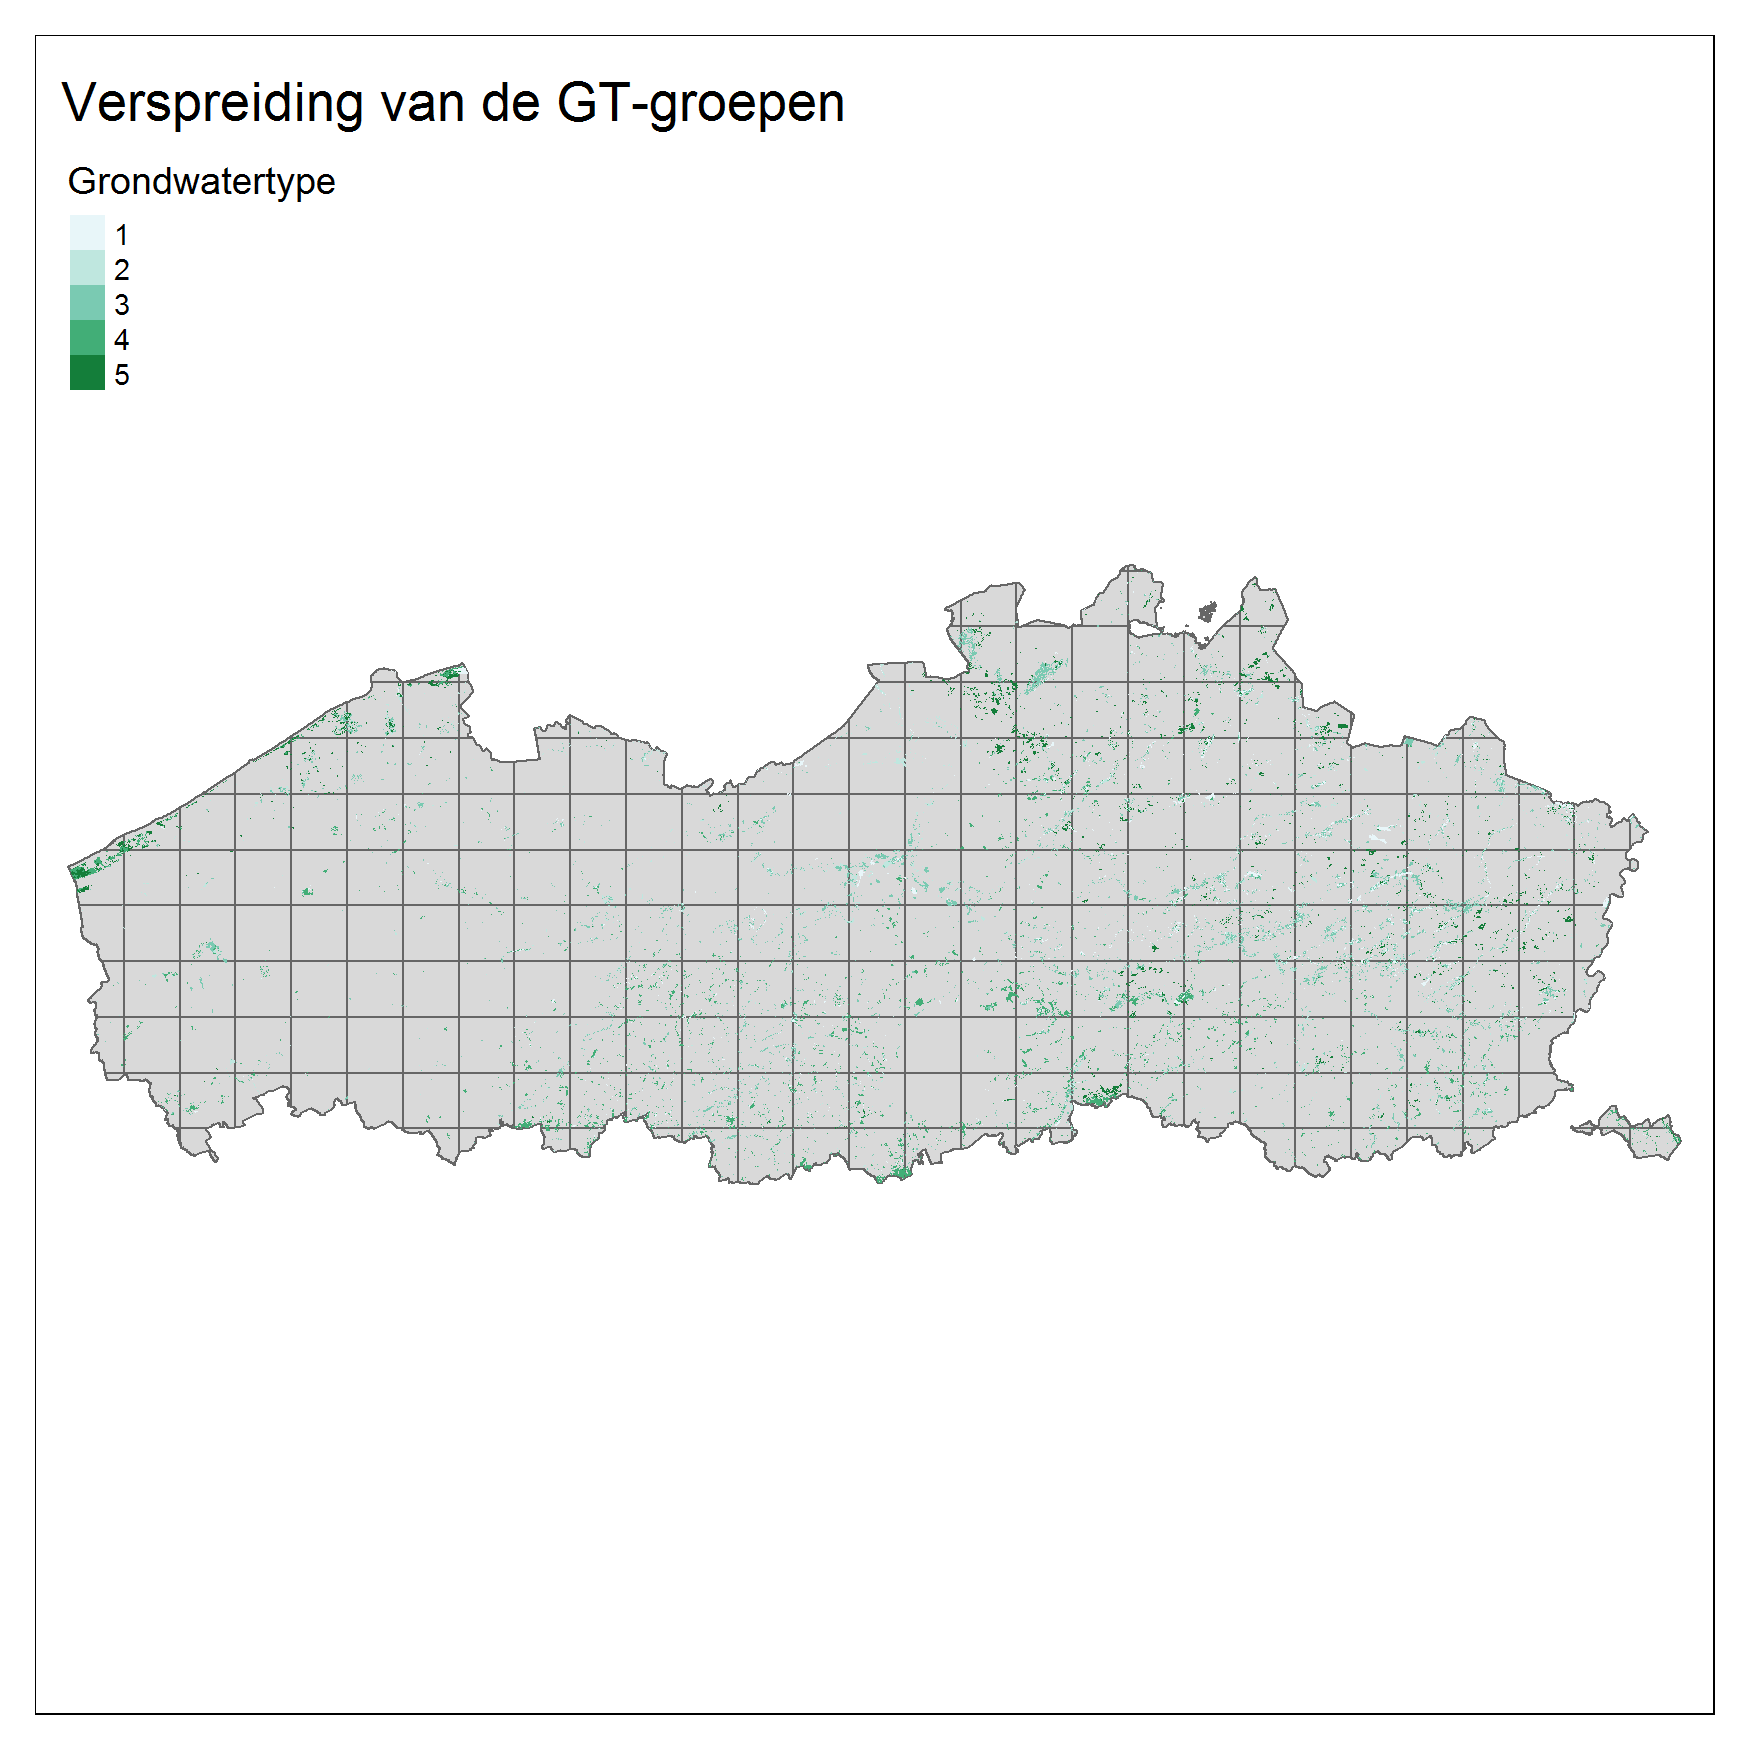
\includegraphics[width=9.41in]{./figures/local/habmap_gw_raster_overlay} \caption{verspreiding-GT-groepen}\label{fig:overlay-habitatkaart-GRTS-plot}
\end{figure}

Tabel \ref{tab:totopp-gw-groep} geeft weer hoeveel de totale oppervlakte
van een GT-groep bedraagt.

\begin{table}

\caption{\label{tab:totopp-gw-groep}Totale oppervlakte van een GT-groep}
\centering
\begin{tabular}[t]{r|r}
\hline
GTgroep & oppervlakte\\
\hline
1 & 4450.660 [ha]\\
\hline
2 & 3285.134 [ha]\\
\hline
3 & 13688.846 [ha]\\
\hline
4 & 12141.519 [ha]\\
\hline
5 & 6080.891 [ha]\\
\hline
\end{tabular}
\end{table}

We kunnen ook per rastercel de (absolute) oppervlakte van een GT-groep
berekenen (tabel \ref{tab:oppGTpercel}).

\begin{table}

\caption{\label{tab:oppGTpercel}Oppervlakte van een GT-groep in een rastercel}
\centering
\begin{tabular}[t]{r|r|r}
\hline
rastercelnummer & GTgroep & oppervlakte\\
\hline
1 & 2 & 13.765220 [ha]\\
\hline
1 & 3 & 45.498443 [ha]\\
\hline
1 & 4 & 14.251735 [ha]\\
\hline
1 & 5 & 207.558727 [ha]\\
\hline
6 & 1 & 1.132350 [ha]\\
\hline
6 & 2 & 7.499600 [ha]\\
\hline
6 & 3 & 14.047280 [ha]\\
\hline
6 & 4 & 44.836180 [ha]\\
\hline
9 & 2 & 5.536500 [ha]\\
\hline
9 & 3 & 2.886390 [ha]\\
\hline
18 & 1 & 19.224135 [ha]\\
\hline
18 & 2 & 18.339650 [ha]\\
\hline
18 & 3 & 55.401100 [ha]\\
\hline
18 & 4 & 0.061020 [ha]\\
\hline
18 & 5 & 41.885910 [ha]\\
\hline
22 & 1 & 9.565080 [ha]\\
\hline
22 & 2 & 17.069150 [ha]\\
\hline
22 & 3 & 31.730360 [ha]\\
\hline
22 & 4 & 36.299080 [ha]\\
\hline
25 & 1 & 29.318335 [ha]\\
\hline
25 & 2 & 3.715830 [ha]\\
\hline
25 & 3 & 16.557380 [ha]\\
\hline
25 & 4 & 268.709735 [ha]\\
\hline
30 & 2 & 4.773820 [ha]\\
\hline
30 & 3 & 0.196000 [ha]\\
\hline
33 & 1 & 1.251900 [ha]\\
\hline
33 & 2 & 0.273500 [ha]\\
\hline
33 & 3 & 2.194220 [ha]\\
\hline
33 & 4 & 21.361350 [ha]\\
\hline
38 & 2 & 0.197000 [ha]\\
\hline
38 & 3 & 1.402400 [ha]\\
\hline
38 & 4 & 43.720590 [ha]\\
\hline
41 & 1 & 0.019900 [ha]\\
\hline
41 & 2 & 69.200960 [ha]\\
\hline
41 & 3 & 0.102600 [ha]\\
\hline
46 & 1 & 50.971950 [ha]\\
\hline
46 & 2 & 12.902180 [ha]\\
\hline
46 & 3 & 45.163635 [ha]\\
\hline
46 & 4 & 11.343725 [ha]\\
\hline
46 & 5 & 181.074285 [ha]\\
\hline
50 & 1 & 1.757990 [ha]\\
\hline
50 & 2 & 8.170770 [ha]\\
\hline
50 & 3 & 129.444820 [ha]\\
\hline
50 & 4 & 129.277375 [ha]\\
\hline
50 & 5 & 30.731995 [ha]\\
\hline
53 & 1 & 0.176520 [ha]\\
\hline
53 & 2 & 29.887810 [ha]\\
\hline
53 & 3 & 14.514942 [ha]\\
\hline
53 & 4 & 47.630315 [ha]\\
\hline
53 & 5 & 95.343175 [ha]\\
\hline
54 & 1 & 57.334899 [ha]\\
\hline
54 & 2 & 54.623470 [ha]\\
\hline
54 & 3 & 270.411125 [ha]\\
\hline
54 & 4 & 8.523770 [ha]\\
\hline
54 & 5 & 69.881860 [ha]\\
\hline
57 & 1 & 9.949820 [ha]\\
\hline
57 & 2 & 10.382500 [ha]\\
\hline
57 & 3 & 93.767080 [ha]\\
\hline
57 & 4 & 196.905040 [ha]\\
\hline
57 & 5 & 8.573900 [ha]\\
\hline
65 & 1 & 3.602500 [ha]\\
\hline
65 & 2 & 0.734500 [ha]\\
\hline
65 & 3 & 33.684058 [ha]\\
\hline
65 & 4 & 24.228009 [ha]\\
\hline
73 & 2 & 16.969290 [ha]\\
\hline
73 & 3 & 8.185540 [ha]\\
\hline
73 & 5 & 4.696600 [ha]\\
\hline
81 & 4 & 1.183060 [ha]\\
\hline
82 & 1 & 12.807305 [ha]\\
\hline
82 & 2 & 12.432825 [ha]\\
\hline
82 & 3 & 57.204985 [ha]\\
\hline
82 & 4 & 1.054765 [ha]\\
\hline
82 & 5 & 61.714505 [ha]\\
\hline
86 & 1 & 29.237050 [ha]\\
\hline
86 & 2 & 2.123130 [ha]\\
\hline
86 & 3 & 98.336700 [ha]\\
\hline
86 & 4 & 22.017900 [ha]\\
\hline
86 & 5 & 5.169190 [ha]\\
\hline
89 & 1 & 6.504005 [ha]\\
\hline
89 & 2 & 3.551580 [ha]\\
\hline
89 & 3 & 66.703280 [ha]\\
\hline
89 & 4 & 188.659495 [ha]\\
\hline
94 & 1 & 8.729798 [ha]\\
\hline
94 & 2 & 0.966400 [ha]\\
\hline
94 & 3 & 21.685570 [ha]\\
\hline
94 & 4 & 5.125162 [ha]\\
\hline
94 & 5 & 18.232650 [ha]\\
\hline
97 & 2 & 0.689020 [ha]\\
\hline
97 & 3 & 8.134700 [ha]\\
\hline
97 & 4 & 4.499600 [ha]\\
\hline
102 & 1 & 0.109560 [ha]\\
\hline
102 & 2 & 11.180690 [ha]\\
\hline
102 & 3 & 15.776150 [ha]\\
\hline
102 & 4 & 13.702240 [ha]\\
\hline
105 & 1 & 25.443920 [ha]\\
\hline
105 & 2 & 10.133975 [ha]\\
\hline
105 & 3 & 86.442925 [ha]\\
\hline
105 & 4 & 28.650940 [ha]\\
\hline
113 & 2 & 19.879610 [ha]\\
\hline
113 & 3 & 19.022940 [ha]\\
\hline
113 & 4 & 17.947295 [ha]\\
\hline
113 & 5 & 125.695312 [ha]\\
\hline
114 & 1 & 8.799360 [ha]\\
\hline
114 & 2 & 41.489150 [ha]\\
\hline
114 & 3 & 112.017865 [ha]\\
\hline
114 & 4 & 134.027450 [ha]\\
\hline
118 & 1 & 88.852960 [ha]\\
\hline
118 & 2 & 27.439690 [ha]\\
\hline
118 & 3 & 106.543560 [ha]\\
\hline
118 & 4 & 1.704280 [ha]\\
\hline
118 & 5 & 69.286810 [ha]\\
\hline
121 & 1 & 14.219560 [ha]\\
\hline
121 & 2 & 2.082460 [ha]\\
\hline
121 & 3 & 57.379890 [ha]\\
\hline
121 & 4 & 134.960200 [ha]\\
\hline
129 & 3 & 1.751640 [ha]\\
\hline
130 & 1 & 0.039360 [ha]\\
\hline
130 & 3 & 3.809880 [ha]\\
\hline
130 & 4 & 18.349040 [ha]\\
\hline
130 & 5 & 10.762880 [ha]\\
\hline
134 & 1 & 80.385645 [ha]\\
\hline
134 & 2 & 10.860760 [ha]\\
\hline
134 & 3 & 121.348145 [ha]\\
\hline
134 & 4 & 221.573845 [ha]\\
\hline
134 & 5 & 161.519755 [ha]\\
\hline
137 & 1 & 5.546160 [ha]\\
\hline
137 & 2 & 4.214030 [ha]\\
\hline
137 & 3 & 20.256110 [ha]\\
\hline
145 & 2 & 1.897600 [ha]\\
\hline
145 & 3 & 2.092200 [ha]\\
\hline
145 & 4 & 0.498300 [ha]\\
\hline
146 & 1 & 157.632145 [ha]\\
\hline
146 & 2 & 28.873085 [ha]\\
\hline
146 & 3 & 65.362695 [ha]\\
\hline
146 & 4 & 0.504485 [ha]\\
\hline
146 & 5 & 83.611310 [ha]\\
\hline
150 & 1 & 37.598830 [ha]\\
\hline
150 & 2 & 40.226100 [ha]\\
\hline
150 & 3 & 141.429700 [ha]\\
\hline
150 & 4 & 108.666280 [ha]\\
\hline
150 & 5 & 52.796285 [ha]\\
\hline
153 & 1 & 1.016313 [ha]\\
\hline
153 & 2 & 19.867390 [ha]\\
\hline
153 & 3 & 66.496045 [ha]\\
\hline
153 & 4 & 112.016077 [ha]\\
\hline
153 & 5 & 0.311560 [ha]\\
\hline
158 & 1 & 13.881710 [ha]\\
\hline
158 & 2 & 1.646880 [ha]\\
\hline
158 & 3 & 30.815435 [ha]\\
\hline
158 & 4 & 2.587560 [ha]\\
\hline
158 & 5 & 54.571620 [ha]\\
\hline
161 & 1 & 0.993100 [ha]\\
\hline
161 & 2 & 1.235410 [ha]\\
\hline
161 & 3 & 8.498970 [ha]\\
\hline
161 & 4 & 18.636920 [ha]\\
\hline
166 & 1 & 7.294320 [ha]\\
\hline
166 & 2 & 70.080660 [ha]\\
\hline
166 & 3 & 76.874865 [ha]\\
\hline
166 & 4 & 74.466355 [ha]\\
\hline
166 & 5 & 0.080880 [ha]\\
\hline
169 & 1 & 0.129600 [ha]\\
\hline
169 & 2 & 29.092840 [ha]\\
\hline
169 & 3 & 137.708720 [ha]\\
\hline
169 & 4 & 13.241490 [ha]\\
\hline
177 & 2 & 1.449480 [ha]\\
\hline
177 & 3 & 3.907140 [ha]\\
\hline
177 & 4 & 507.534625 [ha]\\
\hline
177 & 5 & 237.702411 [ha]\\
\hline
178 & 2 & 0.087480 [ha]\\
\hline
178 & 3 & 0.030240 [ha]\\
\hline
178 & 4 & 22.497675 [ha]\\
\hline
182 & 1 & 73.446780 [ha]\\
\hline
182 & 2 & 27.872310 [ha]\\
\hline
182 & 3 & 124.077040 [ha]\\
\hline
182 & 4 & 1.254960 [ha]\\
\hline
182 & 5 & 19.758220 [ha]\\
\hline
185 & 1 & 13.967255 [ha]\\
\hline
185 & 2 & 8.310390 [ha]\\
\hline
185 & 3 & 29.442930 [ha]\\
\hline
185 & 4 & 423.790225 [ha]\\
\hline
185 & 5 & 4.334620 [ha]\\
\hline
189 & 1 & 6.419000 [ha]\\
\hline
189 & 2 & 17.390370 [ha]\\
\hline
193 & 1 & 2.492950 [ha]\\
\hline
193 & 2 & 1.605570 [ha]\\
\hline
193 & 3 & 45.327145 [ha]\\
\hline
193 & 4 & 26.022940 [ha]\\
\hline
198 & 1 & 22.594930 [ha]\\
\hline
198 & 2 & 11.209715 [ha]\\
\hline
198 & 3 & 76.939550 [ha]\\
\hline
198 & 4 & 432.542115 [ha]\\
\hline
198 & 5 & 3.051550 [ha]\\
\hline
201 & 1 & 7.833140 [ha]\\
\hline
201 & 2 & 11.320650 [ha]\\
\hline
201 & 3 & 124.301780 [ha]\\
\hline
201 & 4 & 12.595910 [ha]\\
\hline
201 & 5 & 1.838800 [ha]\\
\hline
209 & 2 & 0.592890 [ha]\\
\hline
209 & 3 & 24.708770 [ha]\\
\hline
209 & 4 & 8.499260 [ha]\\
\hline
210 & 1 & 34.578574 [ha]\\
\hline
210 & 2 & 5.889380 [ha]\\
\hline
210 & 3 & 172.725420 [ha]\\
\hline
210 & 4 & 5.722580 [ha]\\
\hline
210 & 5 & 73.809385 [ha]\\
\hline
214 & 1 & 40.903675 [ha]\\
\hline
214 & 2 & 33.514605 [ha]\\
\hline
214 & 3 & 116.326800 [ha]\\
\hline
214 & 4 & 156.724005 [ha]\\
\hline
214 & 5 & 47.629000 [ha]\\
\hline
217 & 1 & 15.808300 [ha]\\
\hline
217 & 2 & 16.284100 [ha]\\
\hline
217 & 3 & 164.589290 [ha]\\
\hline
217 & 4 & 194.793040 [ha]\\
\hline
222 & 1 & 9.952665 [ha]\\
\hline
222 & 2 & 0.957150 [ha]\\
\hline
222 & 3 & 147.280371 [ha]\\
\hline
222 & 4 & 0.045200 [ha]\\
\hline
222 & 5 & 91.446000 [ha]\\
\hline
225 & 2 & 1.486490 [ha]\\
\hline
225 & 3 & 5.654270 [ha]\\
\hline
225 & 4 & 5.178600 [ha]\\
\hline
230 & 1 & 0.593280 [ha]\\
\hline
230 & 2 & 1.419135 [ha]\\
\hline
230 & 3 & 84.489185 [ha]\\
\hline
230 & 4 & 44.623600 [ha]\\
\hline
230 & 5 & 14.765610 [ha]\\
\hline
233 & 1 & 97.818435 [ha]\\
\hline
233 & 2 & 85.367465 [ha]\\
\hline
233 & 3 & 196.326535 [ha]\\
\hline
233 & 4 & 12.888550 [ha]\\
\hline
241 & 2 & 7.441380 [ha]\\
\hline
241 & 3 & 4.852860 [ha]\\
\hline
241 & 5 & 10.391000 [ha]\\
\hline
242 & 1 & 10.210940 [ha]\\
\hline
242 & 2 & 2.842040 [ha]\\
\hline
242 & 3 & 22.677150 [ha]\\
\hline
242 & 4 & 4.616600 [ha]\\
\hline
242 & 5 & 6.973885 [ha]\\
\hline
246 & 1 & 24.210335 [ha]\\
\hline
246 & 2 & 11.508022 [ha]\\
\hline
246 & 3 & 21.355335 [ha]\\
\hline
246 & 4 & 0.098260 [ha]\\
\hline
246 & 5 & 30.286375 [ha]\\
\hline
249 & 1 & 25.896140 [ha]\\
\hline
249 & 2 & 1.928660 [ha]\\
\hline
249 & 3 & 58.544160 [ha]\\
\hline
249 & 4 & 141.792815 [ha]\\
\hline
253 & 5 & 0.750800 [ha]\\
\hline
257 & 1 & 9.782920 [ha]\\
\hline
257 & 2 & 2.975110 [ha]\\
\hline
257 & 3 & 11.554200 [ha]\\
\hline
257 & 4 & 40.924580 [ha]\\
\hline
262 & 1 & 23.794330 [ha]\\
\hline
262 & 2 & 45.802265 [ha]\\
\hline
262 & 3 & 163.741355 [ha]\\
\hline
262 & 4 & 201.635895 [ha]\\
\hline
265 & 2 & 12.136600 [ha]\\
\hline
265 & 3 & 66.005720 [ha]\\
\hline
265 & 4 & 48.913580 [ha]\\
\hline
265 & 5 & 19.854320 [ha]\\
\hline
273 & 1 & 1.852471 [ha]\\
\hline
273 & 2 & 0.693750 [ha]\\
\hline
273 & 3 & 14.679505 [ha]\\
\hline
273 & 4 & 60.992229 [ha]\\
\hline
273 & 5 & 3.552300 [ha]\\
\hline
274 & 1 & 4.324405 [ha]\\
\hline
274 & 2 & 42.212205 [ha]\\
\hline
274 & 3 & 70.950430 [ha]\\
\hline
274 & 4 & 10.965500 [ha]\\
\hline
274 & 5 & 11.116325 [ha]\\
\hline
278 & 1 & 47.715060 [ha]\\
\hline
278 & 2 & 5.660710 [ha]\\
\hline
278 & 3 & 90.676560 [ha]\\
\hline
278 & 4 & 42.659255 [ha]\\
\hline
278 & 5 & 2.315810 [ha]\\
\hline
281 & 1 & 0.180900 [ha]\\
\hline
281 & 3 & 6.102960 [ha]\\
\hline
281 & 4 & 38.727900 [ha]\\
\hline
285 & 2 & 7.552900 [ha]\\
\hline
285 & 3 & 2.030070 [ha]\\
\hline
285 & 5 & 3.829400 [ha]\\
\hline
289 & 3 & 0.629060 [ha]\\
\hline
294 & 1 & 1.484635 [ha]\\
\hline
294 & 2 & 26.195785 [ha]\\
\hline
294 & 3 & 50.709515 [ha]\\
\hline
294 & 4 & 62.353910 [ha]\\
\hline
294 & 5 & 8.987880 [ha]\\
\hline
297 & 1 & 0.020900 [ha]\\
\hline
297 & 2 & 39.217980 [ha]\\
\hline
297 & 3 & 127.405660 [ha]\\
\hline
297 & 4 & 5.165600 [ha]\\
\hline
302 & 1 & 27.316120 [ha]\\
\hline
302 & 2 & 7.323445 [ha]\\
\hline
302 & 3 & 86.114211 [ha]\\
\hline
302 & 4 & 9.751575 [ha]\\
\hline
302 & 5 & 31.987560 [ha]\\
\hline
306 & 1 & 102.398810 [ha]\\
\hline
306 & 2 & 77.184140 [ha]\\
\hline
306 & 3 & 149.398120 [ha]\\
\hline
306 & 4 & 5.750100 [ha]\\
\hline
306 & 5 & 55.260810 [ha]\\
\hline
309 & 1 & 20.293030 [ha]\\
\hline
309 & 2 & 1.852780 [ha]\\
\hline
309 & 3 & 0.794850 [ha]\\
\hline
309 & 4 & 111.679325 [ha]\\
\hline
309 & 5 & 129.283360 [ha]\\
\hline
310 & 1 & 41.911670 [ha]\\
\hline
310 & 2 & 59.815145 [ha]\\
\hline
310 & 3 & 193.899040 [ha]\\
\hline
310 & 4 & 23.701325 [ha]\\
\hline
310 & 5 & 43.907930 [ha]\\
\hline
313 & 1 & 2.704830 [ha]\\
\hline
313 & 2 & 0.765230 [ha]\\
\hline
313 & 3 & 15.497030 [ha]\\
\hline
313 & 4 & 167.608180 [ha]\\
\hline
313 & 5 & 1.349300 [ha]\\
\hline
321 & 2 & 0.091160 [ha]\\
\hline
321 & 3 & 0.422400 [ha]\\
\hline
321 & 4 & 8.082410 [ha]\\
\hline
326 & 2 & 8.770090 [ha]\\
\hline
326 & 3 & 0.320600 [ha]\\
\hline
326 & 4 & 0.038070 [ha]\\
\hline
329 & 1 & 1.992700 [ha]\\
\hline
329 & 2 & 20.295970 [ha]\\
\hline
329 & 3 & 6.395190 [ha]\\
\hline
337 & 1 & 1.954180 [ha]\\
\hline
337 & 2 & 2.054990 [ha]\\
\hline
337 & 3 & 21.828790 [ha]\\
\hline
337 & 4 & 39.830920 [ha]\\
\hline
338 & 1 & 7.082445 [ha]\\
\hline
338 & 2 & 6.114725 [ha]\\
\hline
338 & 3 & 49.708855 [ha]\\
\hline
338 & 4 & 8.644330 [ha]\\
\hline
338 & 5 & 12.260440 [ha]\\
\hline
342 & 1 & 89.127310 [ha]\\
\hline
342 & 2 & 6.757630 [ha]\\
\hline
342 & 3 & 72.050368 [ha]\\
\hline
342 & 4 & 28.207710 [ha]\\
\hline
342 & 5 & 18.555470 [ha]\\
\hline
345 & 1 & 14.687100 [ha]\\
\hline
345 & 2 & 3.771650 [ha]\\
\hline
345 & 3 & 49.662900 [ha]\\
\hline
345 & 4 & 120.542260 [ha]\\
\hline
350 & 1 & 17.919597 [ha]\\
\hline
350 & 2 & 0.820720 [ha]\\
\hline
350 & 3 & 16.264080 [ha]\\
\hline
350 & 4 & 3.934338 [ha]\\
\hline
350 & 5 & 2.926820 [ha]\\
\hline
358 & 2 & 7.248070 [ha]\\
\hline
358 & 3 & 26.405335 [ha]\\
\hline
358 & 4 & 13.791120 [ha]\\
\hline
361 & 1 & 8.388050 [ha]\\
\hline
361 & 2 & 10.120640 [ha]\\
\hline
361 & 3 & 12.281250 [ha]\\
\hline
361 & 5 & 0.548700 [ha]\\
\hline
369 & 2 & 0.679740 [ha]\\
\hline
369 & 4 & 3.411515 [ha]\\
\hline
369 & 5 & 11.820315 [ha]\\
\hline
370 & 2 & 0.004290 [ha]\\
\hline
370 & 3 & 3.176050 [ha]\\
\hline
370 & 4 & 6.982590 [ha]\\
\hline
370 & 5 & 2.313690 [ha]\\
\hline
374 & 1 & 2.036800 [ha]\\
\hline
374 & 2 & 3.723320 [ha]\\
\hline
374 & 3 & 9.133510 [ha]\\
\hline
374 & 4 & 0.170000 [ha]\\
\hline
374 & 5 & 8.990710 [ha]\\
\hline
377 & 1 & 0.994100 [ha]\\
\hline
377 & 2 & 4.035570 [ha]\\
\hline
377 & 3 & 43.102170 [ha]\\
\hline
377 & 4 & 78.363680 [ha]\\
\hline
377 & 5 & 0.294000 [ha]\\
\hline
381 & 2 & 6.216910 [ha]\\
\hline
381 & 3 & 4.692470 [ha]\\
\hline
385 & 2 & 0.067820 [ha]\\
\hline
385 & 3 & 9.769700 [ha]\\
\hline
385 & 4 & 20.614905 [ha]\\
\hline
390 & 1 & 12.971705 [ha]\\
\hline
390 & 2 & 23.829440 [ha]\\
\hline
390 & 3 & 71.167660 [ha]\\
\hline
390 & 4 & 222.628330 [ha]\\
\hline
390 & 5 & 8.968940 [ha]\\
\hline
393 & 1 & 0.024510 [ha]\\
\hline
393 & 2 & 10.111600 [ha]\\
\hline
393 & 3 & 23.522020 [ha]\\
\hline
393 & 4 & 0.088100 [ha]\\
\hline
401 & 2 & 0.119520 [ha]\\
\hline
401 & 3 & 2.148010 [ha]\\
\hline
401 & 4 & 13.976290 [ha]\\
\hline
402 & 1 & 23.561200 [ha]\\
\hline
402 & 2 & 20.082320 [ha]\\
\hline
402 & 3 & 54.474490 [ha]\\
\hline
402 & 5 & 20.258550 [ha]\\
\hline
406 & 1 & 9.845440 [ha]\\
\hline
406 & 2 & 37.743550 [ha]\\
\hline
406 & 3 & 38.180970 [ha]\\
\hline
406 & 4 & 24.147250 [ha]\\
\hline
406 & 5 & 94.149200 [ha]\\
\hline
409 & 1 & 5.002595 [ha]\\
\hline
409 & 2 & 13.999650 [ha]\\
\hline
409 & 3 & 63.558940 [ha]\\
\hline
409 & 4 & 53.007125 [ha]\\
\hline
414 & 1 & 9.094180 [ha]\\
\hline
414 & 2 & 2.663760 [ha]\\
\hline
414 & 3 & 48.472670 [ha]\\
\hline
414 & 4 & 13.276870 [ha]\\
\hline
414 & 5 & 18.680660 [ha]\\
\hline
417 & 2 & 1.038910 [ha]\\
\hline
417 & 3 & 2.244855 [ha]\\
\hline
417 & 4 & 1.942200 [ha]\\
\hline
418 & 1 & 0.402600 [ha]\\
\hline
418 & 2 & 1.894740 [ha]\\
\hline
418 & 3 & 4.956470 [ha]\\
\hline
422 & 1 & 0.370490 [ha]\\
\hline
422 & 2 & 5.345990 [ha]\\
\hline
422 & 3 & 36.793055 [ha]\\
\hline
422 & 4 & 198.367150 [ha]\\
\hline
422 & 5 & 7.174945 [ha]\\
\hline
425 & 1 & 3.082620 [ha]\\
\hline
425 & 2 & 57.926315 [ha]\\
\hline
425 & 3 & 137.682525 [ha]\\
\hline
425 & 4 & 4.007080 [ha]\\
\hline
433 & 2 & 0.357880 [ha]\\
\hline
434 & 1 & 0.450540 [ha]\\
\hline
434 & 2 & 0.034740 [ha]\\
\hline
434 & 3 & 0.421600 [ha]\\
\hline
434 & 4 & 72.650730 [ha]\\
\hline
434 & 5 & 0.534770 [ha]\\
\hline
437 & 2 & 2.772170 [ha]\\
\hline
437 & 3 & 46.037110 [ha]\\
\hline
437 & 4 & 36.924395 [ha]\\
\hline
437 & 5 & 223.935850 [ha]\\
\hline
438 & 1 & 62.609846 [ha]\\
\hline
438 & 2 & 44.822095 [ha]\\
\hline
438 & 3 & 278.802690 [ha]\\
\hline
438 & 4 & 0.066190 [ha]\\
\hline
438 & 5 & 25.511820 [ha]\\
\hline
441 & 1 & 19.734315 [ha]\\
\hline
441 & 2 & 13.096970 [ha]\\
\hline
441 & 3 & 49.280460 [ha]\\
\hline
441 & 4 & 145.145725 [ha]\\
\hline
441 & 5 & 16.193390 [ha]\\
\hline
445 & 1 & 20.871270 [ha]\\
\hline
445 & 2 & 91.799210 [ha]\\
\hline
445 & 3 & 14.887630 [ha]\\
\hline
445 & 5 & 0.586500 [ha]\\
\hline
449 & 1 & 3.137890 [ha]\\
\hline
449 & 2 & 7.631570 [ha]\\
\hline
449 & 3 & 17.209570 [ha]\\
\hline
449 & 4 & 4.570900 [ha]\\
\hline
449 & 5 & 16.692100 [ha]\\
\hline
454 & 1 & 22.676315 [ha]\\
\hline
454 & 2 & 10.669685 [ha]\\
\hline
454 & 3 & 33.115050 [ha]\\
\hline
454 & 4 & 212.793565 [ha]\\
\hline
454 & 5 & 3.169400 [ha]\\
\hline
457 & 1 & 3.426090 [ha]\\
\hline
457 & 2 & 27.198240 [ha]\\
\hline
457 & 3 & 70.717230 [ha]\\
\hline
457 & 4 & 30.022125 [ha]\\
\hline
465 & 1 & 1.377570 [ha]\\
\hline
465 & 2 & 1.000845 [ha]\\
\hline
465 & 3 & 17.894155 [ha]\\
\hline
465 & 4 & 9.238980 [ha]\\
\hline
466 & 1 & 21.796185 [ha]\\
\hline
466 & 2 & 16.908160 [ha]\\
\hline
466 & 3 & 109.392090 [ha]\\
\hline
466 & 4 & 0.495160 [ha]\\
\hline
466 & 5 & 134.183575 [ha]\\
\hline
470 & 1 & 68.325300 [ha]\\
\hline
470 & 2 & 4.334860 [ha]\\
\hline
470 & 3 & 54.369760 [ha]\\
\hline
470 & 4 & 28.258710 [ha]\\
\hline
470 & 5 & 20.259670 [ha]\\
\hline
473 & 1 & 0.461660 [ha]\\
\hline
473 & 2 & 0.223160 [ha]\\
\hline
473 & 3 & 1.949310 [ha]\\
\hline
473 & 4 & 10.018180 [ha]\\
\hline
478 & 1 & 38.096415 [ha]\\
\hline
478 & 2 & 2.167450 [ha]\\
\hline
478 & 3 & 320.592050 [ha]\\
\hline
478 & 4 & 2.655700 [ha]\\
\hline
478 & 5 & 55.290530 [ha]\\
\hline
481 & 2 & 1.520140 [ha]\\
\hline
481 & 3 & 1.478320 [ha]\\
\hline
481 & 4 & 2.322600 [ha]\\
\hline
482 & 1 & 13.927110 [ha]\\
\hline
482 & 2 & 1.921780 [ha]\\
\hline
482 & 3 & 33.835055 [ha]\\
\hline
486 & 1 & 4.291240 [ha]\\
\hline
486 & 2 & 42.532575 [ha]\\
\hline
486 & 3 & 62.377705 [ha]\\
\hline
486 & 4 & 74.165405 [ha]\\
\hline
486 & 5 & 59.051075 [ha]\\
\hline
489 & 1 & 0.024300 [ha]\\
\hline
489 & 2 & 11.149660 [ha]\\
\hline
489 & 3 & 56.543860 [ha]\\
\hline
489 & 4 & 60.396800 [ha]\\
\hline
497 & 2 & 19.864780 [ha]\\
\hline
497 & 3 & 57.904810 [ha]\\
\hline
497 & 4 & 58.571224 [ha]\\
\hline
497 & 5 & 1.958600 [ha]\\
\hline
498 & 1 & 13.305450 [ha]\\
\hline
498 & 2 & 7.863350 [ha]\\
\hline
498 & 3 & 18.948220 [ha]\\
\hline
498 & 4 & 0.247560 [ha]\\
\hline
498 & 5 & 1.634700 [ha]\\
\hline
502 & 1 & 14.735050 [ha]\\
\hline
502 & 2 & 18.265440 [ha]\\
\hline
502 & 3 & 79.941378 [ha]\\
\hline
502 & 4 & 0.564120 [ha]\\
\hline
502 & 5 & 25.791330 [ha]\\
\hline
505 & 1 & 27.724520 [ha]\\
\hline
505 & 2 & 18.725420 [ha]\\
\hline
505 & 3 & 129.098805 [ha]\\
\hline
505 & 4 & 179.615305 [ha]\\
\hline
505 & 5 & 2.112000 [ha]\\
\hline
513 & 2 & 4.667630 [ha]\\
\hline
513 & 3 & 80.828710 [ha]\\
\hline
513 & 4 & 1.954800 [ha]\\
\hline
513 & 5 & 26.069500 [ha]\\
\hline
518 & 1 & 14.045310 [ha]\\
\hline
518 & 2 & 7.218500 [ha]\\
\hline
518 & 3 & 19.810040 [ha]\\
\hline
518 & 4 & 89.315500 [ha]\\
\hline
518 & 5 & 1.908920 [ha]\\
\hline
521 & 2 & 12.657020 [ha]\\
\hline
521 & 3 & 0.562680 [ha]\\
\hline
530 & 1 & 51.331560 [ha]\\
\hline
530 & 2 & 26.820235 [ha]\\
\hline
530 & 3 & 180.702839 [ha]\\
\hline
530 & 4 & 0.033680 [ha]\\
\hline
530 & 5 & 42.938970 [ha]\\
\hline
534 & 2 & 23.756600 [ha]\\
\hline
534 & 3 & 70.263590 [ha]\\
\hline
534 & 4 & 27.732090 [ha]\\
\hline
537 & 1 & 9.991870 [ha]\\
\hline
537 & 2 & 22.954240 [ha]\\
\hline
537 & 3 & 57.581660 [ha]\\
\hline
537 & 4 & 380.049230 [ha]\\
\hline
537 & 5 & 8.793980 [ha]\\
\hline
545 & 1 & 0.334710 [ha]\\
\hline
545 & 2 & 3.053910 [ha]\\
\hline
545 & 3 & 9.273380 [ha]\\
\hline
545 & 4 & 34.310400 [ha]\\
\hline
550 & 2 & 8.512880 [ha]\\
\hline
550 & 3 & 37.266060 [ha]\\
\hline
550 & 4 & 45.644480 [ha]\\
\hline
550 & 5 & 3.882200 [ha]\\
\hline
553 & 1 & 3.105570 [ha]\\
\hline
553 & 2 & 71.780960 [ha]\\
\hline
553 & 3 & 6.515780 [ha]\\
\hline
558 & 1 & 61.053825 [ha]\\
\hline
558 & 2 & 15.353485 [ha]\\
\hline
558 & 3 & 96.065390 [ha]\\
\hline
558 & 4 & 1.705535 [ha]\\
\hline
558 & 5 & 40.374920 [ha]\\
\hline
561 & 4 & 56.861515 [ha]\\
\hline
561 & 5 & 11.461925 [ha]\\
\hline
562 & 1 & 32.391730 [ha]\\
\hline
562 & 2 & 19.230840 [ha]\\
\hline
562 & 3 & 40.682475 [ha]\\
\hline
562 & 4 & 5.019800 [ha]\\
\hline
562 & 5 & 55.718580 [ha]\\
\hline
565 & 1 & 85.596804 [ha]\\
\hline
565 & 2 & 2.931290 [ha]\\
\hline
565 & 3 & 0.566630 [ha]\\
\hline
565 & 4 & 3.410800 [ha]\\
\hline
565 & 5 & 8.579800 [ha]\\
\hline
566 & 1 & 70.857595 [ha]\\
\hline
566 & 2 & 11.999810 [ha]\\
\hline
566 & 3 & 77.536910 [ha]\\
\hline
566 & 4 & 12.976345 [ha]\\
\hline
566 & 5 & 22.650900 [ha]\\
\hline
569 & 1 & 9.202910 [ha]\\
\hline
569 & 2 & 3.525750 [ha]\\
\hline
569 & 3 & 54.830425 [ha]\\
\hline
569 & 4 & 88.727260 [ha]\\
\hline
569 & 5 & 1.183080 [ha]\\
\hline
577 & 2 & 2.161050 [ha]\\
\hline
577 & 3 & 19.404070 [ha]\\
\hline
577 & 4 & 45.077950 [ha]\\
\hline
577 & 5 & 3.888100 [ha]\\
\hline
582 & 1 & 6.970710 [ha]\\
\hline
582 & 2 & 22.323250 [ha]\\
\hline
582 & 3 & 34.478820 [ha]\\
\hline
582 & 4 & 299.006910 [ha]\\
\hline
582 & 5 & 161.743870 [ha]\\
\hline
585 & 1 & 12.710670 [ha]\\
\hline
585 & 2 & 0.643960 [ha]\\
\hline
585 & 3 & 15.876540 [ha]\\
\hline
585 & 4 & 2.275170 [ha]\\
\hline
594 & 1 & 34.426245 [ha]\\
\hline
594 & 2 & 14.250969 [ha]\\
\hline
594 & 3 & 26.984640 [ha]\\
\hline
594 & 4 & 2.709460 [ha]\\
\hline
594 & 5 & 107.522540 [ha]\\
\hline
598 & 1 & 12.364650 [ha]\\
\hline
598 & 2 & 14.895080 [ha]\\
\hline
598 & 3 & 71.426510 [ha]\\
\hline
598 & 4 & 32.980740 [ha]\\
\hline
598 & 5 & 21.566420 [ha]\\
\hline
601 & 1 & 10.323210 [ha]\\
\hline
601 & 2 & 5.210170 [ha]\\
\hline
601 & 3 & 32.197600 [ha]\\
\hline
601 & 4 & 313.842570 [ha]\\
\hline
601 & 5 & 0.349500 [ha]\\
\hline
617 & 1 & 32.043885 [ha]\\
\hline
617 & 2 & 20.228120 [ha]\\
\hline
617 & 3 & 9.992950 [ha]\\
\hline
617 & 4 & 1.219710 [ha]\\
\hline
617 & 5 & 1.007780 [ha]\\
\hline
618 & 1 & 6.956990 [ha]\\
\hline
618 & 2 & 3.572525 [ha]\\
\hline
618 & 3 & 16.660460 [ha]\\
\hline
618 & 5 & 11.192830 [ha]\\
\hline
622 & 1 & 0.266220 [ha]\\
\hline
622 & 2 & 0.000000 [ha]\\
\hline
622 & 3 & 3.382320 [ha]\\
\hline
622 & 5 & 62.264130 [ha]\\
\hline
625 & 2 & 4.381870 [ha]\\
\hline
625 & 3 & 2.006040 [ha]\\
\hline
625 & 4 & 14.707020 [ha]\\
\hline
625 & 5 & 35.312110 [ha]\\
\hline
626 & 1 & 6.132720 [ha]\\
\hline
626 & 2 & 26.365485 [ha]\\
\hline
626 & 3 & 110.291265 [ha]\\
\hline
626 & 4 & 126.099355 [ha]\\
\hline
626 & 5 & 42.031060 [ha]\\
\hline
630 & 1 & 142.067950 [ha]\\
\hline
630 & 2 & 11.689780 [ha]\\
\hline
630 & 3 & 171.784365 [ha]\\
\hline
630 & 5 & 34.207800 [ha]\\
\hline
633 & 1 & 10.301855 [ha]\\
\hline
633 & 2 & 16.823150 [ha]\\
\hline
633 & 3 & 75.876500 [ha]\\
\hline
633 & 4 & 182.503345 [ha]\\
\hline
633 & 5 & 0.736800 [ha]\\
\hline
641 & 1 & 4.359820 [ha]\\
\hline
641 & 2 & 0.074250 [ha]\\
\hline
641 & 3 & 5.230790 [ha]\\
\hline
641 & 4 & 42.363155 [ha]\\
\hline
646 & 1 & 10.735950 [ha]\\
\hline
646 & 2 & 34.856245 [ha]\\
\hline
646 & 3 & 83.448950 [ha]\\
\hline
646 & 4 & 99.542170 [ha]\\
\hline
646 & 5 & 11.952990 [ha]\\
\hline
649 & 1 & 6.416240 [ha]\\
\hline
649 & 2 & 17.366440 [ha]\\
\hline
649 & 3 & 82.272490 [ha]\\
\hline
649 & 4 & 44.266855 [ha]\\
\hline
657 & 1 & 0.543300 [ha]\\
\hline
657 & 2 & 14.140840 [ha]\\
\hline
657 & 3 & 9.796580 [ha]\\
\hline
657 & 4 & 61.200120 [ha]\\
\hline
658 & 1 & 14.759920 [ha]\\
\hline
658 & 2 & 3.854050 [ha]\\
\hline
658 & 3 & 50.992370 [ha]\\
\hline
658 & 5 & 0.943530 [ha]\\
\hline
662 & 2 & 1.723900 [ha]\\
\hline
662 & 3 & 4.657310 [ha]\\
\hline
662 & 4 & 74.343340 [ha]\\
\hline
665 & 1 & 1.287930 [ha]\\
\hline
665 & 2 & 2.214340 [ha]\\
\hline
665 & 3 & 4.712180 [ha]\\
\hline
665 & 4 & 15.301530 [ha]\\
\hline
670 & 1 & 8.399620 [ha]\\
\hline
670 & 2 & 9.755810 [ha]\\
\hline
670 & 3 & 51.672805 [ha]\\
\hline
670 & 4 & 14.097890 [ha]\\
\hline
670 & 5 & 89.949230 [ha]\\
\hline
673 & 2 & 6.475580 [ha]\\
\hline
673 & 3 & 7.283820 [ha]\\
\hline
673 & 4 & 12.289200 [ha]\\
\hline
678 & 2 & 8.398900 [ha]\\
\hline
678 & 3 & 22.873380 [ha]\\
\hline
678 & 4 & 85.684135 [ha]\\
\hline
678 & 5 & 12.308220 [ha]\\
\hline
681 & 1 & 48.273865 [ha]\\
\hline
681 & 2 & 21.111000 [ha]\\
\hline
681 & 3 & 104.012830 [ha]\\
\hline
681 & 4 & 32.964485 [ha]\\
\hline
689 & 2 & 0.850990 [ha]\\
\hline
690 & 3 & 0.348780 [ha]\\
\hline
690 & 4 & 8.304640 [ha]\\
\hline
690 & 5 & 0.457190 [ha]\\
\hline
693 & 1 & 6.419180 [ha]\\
\hline
693 & 2 & 49.448520 [ha]\\
\hline
693 & 3 & 156.354850 [ha]\\
\hline
693 & 4 & 5.952320 [ha]\\
\hline
693 & 5 & 226.529150 [ha]\\
\hline
694 & 1 & 140.630036 [ha]\\
\hline
694 & 2 & 82.202733 [ha]\\
\hline
694 & 3 & 283.597829 [ha]\\
\hline
694 & 4 & 6.117355 [ha]\\
\hline
694 & 5 & 78.914885 [ha]\\
\hline
697 & 1 & 2.993900 [ha]\\
\hline
697 & 2 & 1.294520 [ha]\\
\hline
697 & 3 & 7.524950 [ha]\\
\hline
697 & 4 & 40.753800 [ha]\\
\hline
701 & 2 & 7.028700 [ha]\\
\hline
701 & 3 & 33.495490 [ha]\\
\hline
701 & 5 & 27.272520 [ha]\\
\hline
705 & 2 & 2.133110 [ha]\\
\hline
705 & 3 & 1.900980 [ha]\\
\hline
705 & 4 & 2.320370 [ha]\\
\hline
710 & 1 & 2.777400 [ha]\\
\hline
710 & 2 & 0.671640 [ha]\\
\hline
710 & 3 & 36.937120 [ha]\\
\hline
710 & 4 & 258.730195 [ha]\\
\hline
710 & 5 & 3.528150 [ha]\\
\hline
713 & 1 & 11.413655 [ha]\\
\hline
713 & 2 & 4.850370 [ha]\\
\hline
713 & 3 & 24.729755 [ha]\\
\hline
713 & 4 & 27.138645 [ha]\\
\hline
721 & 2 & 7.330025 [ha]\\
\hline
721 & 3 & 2.810895 [ha]\\
\hline
721 & 4 & 17.716300 [ha]\\
\hline
721 & 5 & 4.545600 [ha]\\
\hline
722 & 1 & 175.947505 [ha]\\
\hline
722 & 2 & 43.036815 [ha]\\
\hline
722 & 3 & 269.677680 [ha]\\
\hline
722 & 4 & 1.436070 [ha]\\
\hline
722 & 5 & 59.793655 [ha]\\
\hline
726 & 1 & 38.763880 [ha]\\
\hline
726 & 2 & 10.880135 [ha]\\
\hline
726 & 3 & 51.294890 [ha]\\
\hline
726 & 4 & 17.079930 [ha]\\
\hline
726 & 5 & 69.898915 [ha]\\
\hline
729 & 1 & 3.215500 [ha]\\
\hline
729 & 2 & 8.646500 [ha]\\
\hline
729 & 3 & 85.145510 [ha]\\
\hline
729 & 4 & 88.621440 [ha]\\
\hline
734 & 1 & 10.542400 [ha]\\
\hline
734 & 2 & 3.423120 [ha]\\
\hline
734 & 3 & 410.827364 [ha]\\
\hline
734 & 4 & 0.600800 [ha]\\
\hline
734 & 5 & 156.688260 [ha]\\
\hline
737 & 2 & 1.396100 [ha]\\
\hline
737 & 3 & 0.482780 [ha]\\
\hline
737 & 4 & 4.546990 [ha]\\
\hline
742 & 1 & 47.632729 [ha]\\
\hline
742 & 2 & 36.505424 [ha]\\
\hline
742 & 3 & 140.892311 [ha]\\
\hline
742 & 4 & 45.109540 [ha]\\
\hline
742 & 5 & 11.591525 [ha]\\
\hline
745 & 1 & 43.929390 [ha]\\
\hline
745 & 2 & 54.338150 [ha]\\
\hline
745 & 3 & 522.583745 [ha]\\
\hline
745 & 4 & 53.248085 [ha]\\
\hline
750 & 1 & 40.677550 [ha]\\
\hline
750 & 2 & 14.789355 [ha]\\
\hline
750 & 3 & 63.422110 [ha]\\
\hline
750 & 4 & 1.932395 [ha]\\
\hline
750 & 5 & 94.016650 [ha]\\
\hline
753 & 3 & 0.122400 [ha]\\
\hline
753 & 4 & 3.071400 [ha]\\
\hline
754 & 1 & 0.126330 [ha]\\
\hline
754 & 3 & 0.271840 [ha]\\
\hline
758 & 1 & 69.878725 [ha]\\
\hline
758 & 2 & 19.192510 [ha]\\
\hline
758 & 3 & 70.318160 [ha]\\
\hline
758 & 4 & 2.220990 [ha]\\
\hline
758 & 5 & 10.981470 [ha]\\
\hline
761 & 1 & 4.720560 [ha]\\
\hline
761 & 2 & 13.475120 [ha]\\
\hline
761 & 3 & 101.317815 [ha]\\
\hline
761 & 4 & 85.816365 [ha]\\
\hline
769 & 1 & 2.070240 [ha]\\
\hline
769 & 2 & 1.628720 [ha]\\
\hline
769 & 3 & 15.127710 [ha]\\
\hline
769 & 4 & 19.488615 [ha]\\
\hline
769 & 5 & 13.139300 [ha]\\
\hline
774 & 1 & 0.370690 [ha]\\
\hline
774 & 2 & 0.761190 [ha]\\
\hline
774 & 4 & 23.251340 [ha]\\
\hline
777 & 1 & 5.794300 [ha]\\
\hline
777 & 2 & 57.282040 [ha]\\
\hline
777 & 3 & 19.766115 [ha]\\
\hline
777 & 5 & 15.124140 [ha]\\
\hline
785 & 4 & 0.305930 [ha]\\
\hline
786 & 1 & 43.728020 [ha]\\
\hline
786 & 2 & 17.640425 [ha]\\
\hline
786 & 3 & 50.001695 [ha]\\
\hline
786 & 5 & 57.933920 [ha]\\
\hline
790 & 1 & 8.171690 [ha]\\
\hline
790 & 2 & 16.302370 [ha]\\
\hline
790 & 3 & 110.036490 [ha]\\
\hline
790 & 4 & 32.464230 [ha]\\
\hline
793 & 1 & 3.822950 [ha]\\
\hline
793 & 2 & 0.921100 [ha]\\
\hline
793 & 3 & 7.168880 [ha]\\
\hline
793 & 4 & 66.657710 [ha]\\
\hline
797 & 2 & 6.561560 [ha]\\
\hline
797 & 3 & 1.109410 [ha]\\
\hline
798 & 2 & 1.467200 [ha]\\
\hline
798 & 3 & 3.094690 [ha]\\
\hline
798 & 5 & 13.660670 [ha]\\
\hline
801 & 4 & 13.802800 [ha]\\
\hline
806 & 2 & 4.166440 [ha]\\
\hline
806 & 3 & 8.381680 [ha]\\
\hline
806 & 4 & 66.333170 [ha]\\
\hline
809 & 3 & 0.837000 [ha]\\
\hline
809 & 4 & 0.511800 [ha]\\
\hline
814 & 1 & 17.044595 [ha]\\
\hline
814 & 2 & 3.765830 [ha]\\
\hline
814 & 3 & 35.883620 [ha]\\
\hline
814 & 4 & 5.221730 [ha]\\
\hline
814 & 5 & 125.556270 [ha]\\
\hline
817 & 1 & 13.828190 [ha]\\
\hline
817 & 2 & 6.527450 [ha]\\
\hline
817 & 3 & 7.281750 [ha]\\
\hline
817 & 4 & 204.870085 [ha]\\
\hline
817 & 5 & 165.005785 [ha]\\
\hline
818 & 1 & 12.287490 [ha]\\
\hline
818 & 2 & 34.756890 [ha]\\
\hline
818 & 3 & 130.269730 [ha]\\
\hline
818 & 4 & 133.817560 [ha]\\
\hline
818 & 5 & 10.990480 [ha]\\
\hline
821 & 2 & 8.839865 [ha]\\
\hline
821 & 3 & 4.060180 [ha]\\
\hline
822 & 1 & 97.111260 [ha]\\
\hline
822 & 2 & 18.061684 [ha]\\
\hline
822 & 3 & 251.577684 [ha]\\
\hline
822 & 4 & 39.927635 [ha]\\
\hline
822 & 5 & 39.518695 [ha]\\
\hline
825 & 1 & 22.492340 [ha]\\
\hline
825 & 2 & 11.644685 [ha]\\
\hline
825 & 3 & 71.962600 [ha]\\
\hline
825 & 4 & 130.318860 [ha]\\
\hline
825 & 5 & 7.049240 [ha]\\
\hline
833 & 1 & 8.727795 [ha]\\
\hline
833 & 2 & 2.508040 [ha]\\
\hline
833 & 3 & 17.644980 [ha]\\
\hline
833 & 4 & 16.600015 [ha]\\
\hline
838 & 1 & 1.189400 [ha]\\
\hline
838 & 2 & 18.554940 [ha]\\
\hline
838 & 3 & 47.855545 [ha]\\
\hline
838 & 4 & 99.246880 [ha]\\
\hline
838 & 5 & 4.510480 [ha]\\
\hline
841 & 2 & 1.146910 [ha]\\
\hline
841 & 3 & 7.958020 [ha]\\
\hline
841 & 4 & 0.981590 [ha]\\
\hline
849 & 1 & 1.814217 [ha]\\
\hline
849 & 2 & 1.676500 [ha]\\
\hline
849 & 3 & 13.717085 [ha]\\
\hline
849 & 4 & 124.110263 [ha]\\
\hline
849 & 5 & 2.657800 [ha]\\
\hline
850 & 1 & 76.257100 [ha]\\
\hline
850 & 2 & 12.921610 [ha]\\
\hline
850 & 3 & 63.148945 [ha]\\
\hline
850 & 4 & 7.299325 [ha]\\
\hline
850 & 5 & 104.792235 [ha]\\
\hline
854 & 1 & 58.395345 [ha]\\
\hline
854 & 2 & 3.187220 [ha]\\
\hline
854 & 3 & 49.094810 [ha]\\
\hline
854 & 4 & 15.882120 [ha]\\
\hline
857 & 1 & 9.502330 [ha]\\
\hline
857 & 2 & 3.430030 [ha]\\
\hline
857 & 3 & 35.791670 [ha]\\
\hline
857 & 4 & 235.096820 [ha]\\
\hline
862 & 1 & 0.226480 [ha]\\
\hline
862 & 2 & 0.065100 [ha]\\
\hline
862 & 3 & 0.208520 [ha]\\
\hline
862 & 4 & 0.273460 [ha]\\
\hline
865 & 2 & 0.173440 [ha]\\
\hline
865 & 3 & 1.547680 [ha]\\
\hline
865 & 4 & 1.279650 [ha]\\
\hline
870 & 3 & 3.344800 [ha]\\
\hline
870 & 4 & 12.004500 [ha]\\
\hline
873 & 2 & 1.625820 [ha]\\
\hline
873 & 3 & 0.690900 [ha]\\
\hline
874 & 1 & 5.983700 [ha]\\
\hline
874 & 2 & 3.374730 [ha]\\
\hline
874 & 3 & 1.821780 [ha]\\
\hline
874 & 5 & 3.368000 [ha]\\
\hline
878 & 2 & 0.051820 [ha]\\
\hline
878 & 3 & 1.112370 [ha]\\
\hline
878 & 5 & 0.055200 [ha]\\
\hline
881 & 2 & 9.521980 [ha]\\
\hline
881 & 3 & 11.632610 [ha]\\
\hline
881 & 5 & 32.089450 [ha]\\
\hline
882 & 4 & 15.269330 [ha]\\
\hline
886 & 1 & 85.728335 [ha]\\
\hline
886 & 2 & 51.063750 [ha]\\
\hline
886 & 3 & 187.574865 [ha]\\
\hline
886 & 4 & 0.506800 [ha]\\
\hline
886 & 5 & 20.747480 [ha]\\
\hline
889 & 4 & 0.089400 [ha]\\
\hline
897 & 2 & 5.685020 [ha]\\
\hline
897 & 3 & 3.639720 [ha]\\
\hline
897 & 4 & 2.442600 [ha]\\
\hline
898 & 1 & 7.132070 [ha]\\
\hline
898 & 2 & 1.674180 [ha]\\
\hline
898 & 3 & 17.336210 [ha]\\
\hline
898 & 4 & 88.972000 [ha]\\
\hline
898 & 5 & 36.505910 [ha]\\
\hline
902 & 1 & 9.465840 [ha]\\
\hline
902 & 2 & 16.302415 [ha]\\
\hline
902 & 3 & 150.450661 [ha]\\
\hline
902 & 4 & 127.185120 [ha]\\
\hline
902 & 5 & 30.626255 [ha]\\
\hline
905 & 1 & 5.417980 [ha]\\
\hline
905 & 2 & 16.836165 [ha]\\
\hline
905 & 3 & 92.040680 [ha]\\
\hline
905 & 4 & 32.945295 [ha]\\
\hline
913 & 1 & 0.109600 [ha]\\
\hline
913 & 3 & 0.041100 [ha]\\
\hline
913 & 4 & 52.741425 [ha]\\
\hline
918 & 1 & 107.243625 [ha]\\
\hline
918 & 2 & 19.127100 [ha]\\
\hline
918 & 3 & 69.366145 [ha]\\
\hline
918 & 4 & 134.229740 [ha]\\
\hline
918 & 5 & 131.362995 [ha]\\
\hline
921 & 1 & 10.867020 [ha]\\
\hline
921 & 2 & 11.970010 [ha]\\
\hline
921 & 3 & 59.406850 [ha]\\
\hline
921 & 4 & 97.377670 [ha]\\
\hline
926 & 2 & 0.029430 [ha]\\
\hline
926 & 3 & 2.919310 [ha]\\
\hline
926 & 4 & 0.295620 [ha]\\
\hline
929 & 2 & 3.822170 [ha]\\
\hline
929 & 3 & 11.868525 [ha]\\
\hline
929 & 4 & 3.446650 [ha]\\
\hline
934 & 1 & 28.600210 [ha]\\
\hline
934 & 2 & 5.766160 [ha]\\
\hline
934 & 3 & 41.199450 [ha]\\
\hline
934 & 4 & 171.704300 [ha]\\
\hline
934 & 5 & 23.752965 [ha]\\
\hline
937 & 1 & 7.389100 [ha]\\
\hline
937 & 2 & 37.484395 [ha]\\
\hline
937 & 3 & 78.955545 [ha]\\
\hline
937 & 4 & 0.762920 [ha]\\
\hline
945 & 2 & 6.220390 [ha]\\
\hline
945 & 3 & 0.092550 [ha]\\
\hline
945 & 4 & 7.573790 [ha]\\
\hline
945 & 5 & 13.496995 [ha]\\
\hline
946 & 3 & 0.000000 [ha]\\
\hline
949 & 1 & 4.427400 [ha]\\
\hline
950 & 1 & 204.781260 [ha]\\
\hline
950 & 2 & 22.931790 [ha]\\
\hline
950 & 3 & 190.011125 [ha]\\
\hline
950 & 4 & 1.043480 [ha]\\
\hline
950 & 5 & 117.645490 [ha]\\
\hline
953 & 1 & 11.754880 [ha]\\
\hline
953 & 2 & 4.739320 [ha]\\
\hline
953 & 3 & 14.840720 [ha]\\
\hline
953 & 4 & 170.979225 [ha]\\
\hline
953 & 5 & 3.228280 [ha]\\
\hline
957 & 1 & 3.868740 [ha]\\
\hline
957 & 2 & 70.814190 [ha]\\
\hline
957 & 3 & 20.568840 [ha]\\
\hline
957 & 5 & 26.172740 [ha]\\
\hline
961 & 1 & 6.019750 [ha]\\
\hline
961 & 2 & 7.816940 [ha]\\
\hline
961 & 3 & 62.088470 [ha]\\
\hline
961 & 4 & 31.251010 [ha]\\
\hline
961 & 5 & 0.034110 [ha]\\
\hline
966 & 1 & 1.073300 [ha]\\
\hline
966 & 2 & 3.018310 [ha]\\
\hline
966 & 3 & 7.299700 [ha]\\
\hline
966 & 4 & 7.658040 [ha]\\
\hline
969 & 1 & 1.512330 [ha]\\
\hline
969 & 2 & 0.712010 [ha]\\
\hline
969 & 3 & 20.230640 [ha]\\
\hline
969 & 4 & 17.167390 [ha]\\
\hline
977 & 1 & 1.160205 [ha]\\
\hline
977 & 2 & 0.691660 [ha]\\
\hline
977 & 3 & 5.701900 [ha]\\
\hline
977 & 4 & 23.780350 [ha]\\
\hline
978 & 1 & 45.394309 [ha]\\
\hline
978 & 2 & 16.019500 [ha]\\
\hline
978 & 3 & 133.933605 [ha]\\
\hline
978 & 4 & 6.701965 [ha]\\
\hline
978 & 5 & 63.512210 [ha]\\
\hline
982 & 1 & 47.561380 [ha]\\
\hline
982 & 2 & 5.021430 [ha]\\
\hline
982 & 3 & 66.988455 [ha]\\
\hline
982 & 4 & 4.157650 [ha]\\
\hline
982 & 5 & 58.829180 [ha]\\
\hline
985 & 1 & 37.493605 [ha]\\
\hline
985 & 2 & 2.860775 [ha]\\
\hline
985 & 3 & 57.188100 [ha]\\
\hline
985 & 4 & 221.039165 [ha]\\
\hline
985 & 5 & 0.486240 [ha]\\
\hline
990 & 1 & 0.424500 [ha]\\
\hline
990 & 2 & 0.481950 [ha]\\
\hline
990 & 3 & 22.612865 [ha]\\
\hline
990 & 4 & 0.777990 [ha]\\
\hline
990 & 5 & 316.159080 [ha]\\
\hline
993 & 2 & 0.568290 [ha]\\
\hline
993 & 3 & 1.812800 [ha]\\
\hline
993 & 4 & 13.557750 [ha]\\
\hline
998 & 1 & 23.970130 [ha]\\
\hline
998 & 2 & 41.029570 [ha]\\
\hline
998 & 3 & 124.996830 [ha]\\
\hline
998 & 4 & 23.408830 [ha]\\
\hline
998 & 5 & 26.514530 [ha]\\
\hline
1001 & 1 & 2.126680 [ha]\\
\hline
1001 & 3 & 14.266400 [ha]\\
\hline
1001 & 4 & 76.977760 [ha]\\
\hline
1009 & 1 & 0.238840 [ha]\\
\hline
1009 & 2 & 0.450030 [ha]\\
\hline
1009 & 3 & 1.590070 [ha]\\
\hline
1010 & 1 & 68.904335 [ha]\\
\hline
1010 & 2 & 8.527400 [ha]\\
\hline
1010 & 3 & 151.699180 [ha]\\
\hline
1010 & 4 & 1.488645 [ha]\\
\hline
1010 & 5 & 58.084830 [ha]\\
\hline
1014 & 1 & 113.203725 [ha]\\
\hline
1014 & 2 & 4.266135 [ha]\\
\hline
1014 & 3 & 45.793215 [ha]\\
\hline
1014 & 4 & 2.000525 [ha]\\
\hline
1014 & 5 & 61.993275 [ha]\\
\hline
1017 & 1 & 19.509170 [ha]\\
\hline
1017 & 2 & 19.904390 [ha]\\
\hline
1017 & 3 & 218.506420 [ha]\\
\hline
1017 & 4 & 37.257900 [ha]\\
\hline
\end{tabular}
\end{table}

\subsection{Berekening gemiddelde benodigde oppervlakte van een GT-groep
per
meetpunt}\label{berekening-gemiddelde-benodigde-oppervlakte-van-een-gt-groep-per-meetpunt}

We gaan hier uit van de keuze voor een gelijke verdeling van de
meetpunten over de strata (= GT-groepen), namelijk we wensen 20
meetpunten per GT-groep. We kennen de totale oppervlakte van een
GT-groep, de oppervlakte van een GT-groep in elke rastercel en hoeveel
meetpunten er per GT-groep gewenst zijn. Deze gegevens maken volgende
berekeningen mogelijk :

\begin{itemize}
\tightlist
\item
  de minimaal nodige oppervlakte per meetpunt in een GT-groep (tabel
  \ref{tab:gemiddelde-oppervlakte-per-GTgroep});
\item
  het gewenste aantal meetpunten per rastercel (tabel
  \ref{tab:gewenst-aantal-meetpunten-per-raster})
\end{itemize}

Voor dit laatste wordt een iteratie uitgevoerd, zoals beschreven in
\ref{ruimte-sel-raster}.

\begin{table}

\caption{\label{tab:gemiddelde-oppervlakte-per-GTgroep}Minimaal benodigde oppervlakte van een GT-groep per meetpunt en per rastercel}
\centering
\begin{tabular}[t]{r|r|r|r}
\hline
GTgroep & oppervl. GT-groep & min. oppervl. per meetpunt & correctiefactor\\
\hline
1 & 4451 [ha] & 136 [ha] & 0.61\\
\hline
2 & 3285 [ha] & 84 [ha] & 0.51\\
\hline
3 & 13689 [ha] & 308 [ha] & 0.45\\
\hline
4 & 12142 [ha] & 364 [ha] & 0.60\\
\hline
5 & 6081 [ha] & 189 [ha] & 0.62\\
\hline
\end{tabular}
\end{table}

\begin{table}

\caption{\label{tab:gewenst-aantal-meetpunten-per-raster}gewenst aantal meetpunten per GT-groep en per rastercel}
\centering
\begin{tabular}[t]{r|r|r|r|r|r}
\hline
rastercelnummer & GTgroep & GToppervl. in cel & GToppervl. totaal & min. oppervl. per meetpunt & gewenst aantal meetptn\\
\hline
950 & 1 & 205 [ha] & 4451 [ha] & 136 [ha] & 2\\
\hline
722 & 1 & 176 [ha] & 4451 [ha] & 136 [ha] & 1\\
\hline
146 & 1 & 158 [ha] & 4451 [ha] & 136 [ha] & 1\\
\hline
630 & 1 & 142 [ha] & 4451 [ha] & 136 [ha] & 1\\
\hline
694 & 1 & 141 [ha] & 4451 [ha] & 136 [ha] & 1\\
\hline
1014 & 1 & 113 [ha] & 4451 [ha] & 136 [ha] & 1\\
\hline
918 & 1 & 107 [ha] & 4451 [ha] & 136 [ha] & 1\\
\hline
306 & 1 & 102 [ha] & 4451 [ha] & 136 [ha] & 1\\
\hline
233 & 1 & 98 [ha] & 4451 [ha] & 136 [ha] & 1\\
\hline
822 & 1 & 97 [ha] & 4451 [ha] & 136 [ha] & 1\\
\hline
342 & 1 & 89 [ha] & 4451 [ha] & 136 [ha] & 1\\
\hline
118 & 1 & 89 [ha] & 4451 [ha] & 136 [ha] & 1\\
\hline
886 & 1 & 86 [ha] & 4451 [ha] & 136 [ha] & 1\\
\hline
565 & 1 & 86 [ha] & 4451 [ha] & 136 [ha] & 1\\
\hline
134 & 1 & 80 [ha] & 4451 [ha] & 136 [ha] & 1\\
\hline
850 & 1 & 76 [ha] & 4451 [ha] & 136 [ha] & 1\\
\hline
182 & 1 & 73 [ha] & 4451 [ha] & 136 [ha] & 1\\
\hline
566 & 1 & 71 [ha] & 4451 [ha] & 136 [ha] & 1\\
\hline
758 & 1 & 70 [ha] & 4451 [ha] & 136 [ha] & 1\\
\hline
1010 & 1 & 69 [ha] & 4451 [ha] & 136 [ha] & 1\\
\hline
470 & 1 & 68 [ha] & 4451 [ha] & 136 [ha] & 1\\
\hline
445 & 2 & 92 [ha] & 3285 [ha] & 84 [ha] & 1\\
\hline
233 & 2 & 85 [ha] & 3285 [ha] & 84 [ha] & 1\\
\hline
694 & 2 & 82 [ha] & 3285 [ha] & 84 [ha] & 1\\
\hline
306 & 2 & 77 [ha] & 3285 [ha] & 84 [ha] & 1\\
\hline
553 & 2 & 72 [ha] & 3285 [ha] & 84 [ha] & 1\\
\hline
957 & 2 & 71 [ha] & 3285 [ha] & 84 [ha] & 1\\
\hline
166 & 2 & 70 [ha] & 3285 [ha] & 84 [ha] & 1\\
\hline
41 & 2 & 69 [ha] & 3285 [ha] & 84 [ha] & 1\\
\hline
310 & 2 & 60 [ha] & 3285 [ha] & 84 [ha] & 1\\
\hline
425 & 2 & 58 [ha] & 3285 [ha] & 84 [ha] & 1\\
\hline
777 & 2 & 57 [ha] & 3285 [ha] & 84 [ha] & 1\\
\hline
54 & 2 & 55 [ha] & 3285 [ha] & 84 [ha] & 1\\
\hline
745 & 2 & 54 [ha] & 3285 [ha] & 84 [ha] & 1\\
\hline
886 & 2 & 51 [ha] & 3285 [ha] & 84 [ha] & 1\\
\hline
693 & 2 & 49 [ha] & 3285 [ha] & 84 [ha] & 1\\
\hline
262 & 2 & 46 [ha] & 3285 [ha] & 84 [ha] & 1\\
\hline
438 & 2 & 45 [ha] & 3285 [ha] & 84 [ha] & 1\\
\hline
722 & 2 & 43 [ha] & 3285 [ha] & 84 [ha] & 1\\
\hline
486 & 2 & 43 [ha] & 3285 [ha] & 84 [ha] & 1\\
\hline
274 & 2 & 42 [ha] & 3285 [ha] & 84 [ha] & 1\\
\hline
745 & 3 & 523 [ha] & 13689 [ha] & 308 [ha] & 2\\
\hline
734 & 3 & 411 [ha] & 13689 [ha] & 308 [ha] & 1\\
\hline
478 & 3 & 321 [ha] & 13689 [ha] & 308 [ha] & 1\\
\hline
694 & 3 & 284 [ha] & 13689 [ha] & 308 [ha] & 1\\
\hline
438 & 3 & 279 [ha] & 13689 [ha] & 308 [ha] & 1\\
\hline
54 & 3 & 270 [ha] & 13689 [ha] & 308 [ha] & 1\\
\hline
722 & 3 & 270 [ha] & 13689 [ha] & 308 [ha] & 1\\
\hline
822 & 3 & 252 [ha] & 13689 [ha] & 308 [ha] & 1\\
\hline
1017 & 3 & 219 [ha] & 13689 [ha] & 308 [ha] & 1\\
\hline
233 & 3 & 196 [ha] & 13689 [ha] & 308 [ha] & 1\\
\hline
310 & 3 & 194 [ha] & 13689 [ha] & 308 [ha] & 1\\
\hline
950 & 3 & 190 [ha] & 13689 [ha] & 308 [ha] & 1\\
\hline
886 & 3 & 188 [ha] & 13689 [ha] & 308 [ha] & 1\\
\hline
530 & 3 & 181 [ha] & 13689 [ha] & 308 [ha] & 1\\
\hline
210 & 3 & 173 [ha] & 13689 [ha] & 308 [ha] & 1\\
\hline
630 & 3 & 172 [ha] & 13689 [ha] & 308 [ha] & 1\\
\hline
217 & 3 & 165 [ha] & 13689 [ha] & 308 [ha] & 1\\
\hline
262 & 3 & 164 [ha] & 13689 [ha] & 308 [ha] & 1\\
\hline
693 & 3 & 156 [ha] & 13689 [ha] & 308 [ha] & 1\\
\hline
177 & 4 & 508 [ha] & 12142 [ha] & 364 [ha] & 1\\
\hline
198 & 4 & 433 [ha] & 12142 [ha] & 364 [ha] & 1\\
\hline
185 & 4 & 424 [ha] & 12142 [ha] & 364 [ha] & 1\\
\hline
537 & 4 & 380 [ha] & 12142 [ha] & 364 [ha] & 1\\
\hline
601 & 4 & 314 [ha] & 12142 [ha] & 364 [ha] & 1\\
\hline
582 & 4 & 299 [ha] & 12142 [ha] & 364 [ha] & 1\\
\hline
25 & 4 & 269 [ha] & 12142 [ha] & 364 [ha] & 1\\
\hline
710 & 4 & 259 [ha] & 12142 [ha] & 364 [ha] & 1\\
\hline
857 & 4 & 235 [ha] & 12142 [ha] & 364 [ha] & 1\\
\hline
390 & 4 & 223 [ha] & 12142 [ha] & 364 [ha] & 1\\
\hline
134 & 4 & 222 [ha] & 12142 [ha] & 364 [ha] & 1\\
\hline
985 & 4 & 221 [ha] & 12142 [ha] & 364 [ha] & 1\\
\hline
454 & 4 & 213 [ha] & 12142 [ha] & 364 [ha] & 1\\
\hline
817 & 4 & 205 [ha] & 12142 [ha] & 364 [ha] & 1\\
\hline
262 & 4 & 202 [ha] & 12142 [ha] & 364 [ha] & 1\\
\hline
422 & 4 & 198 [ha] & 12142 [ha] & 364 [ha] & 1\\
\hline
57 & 4 & 197 [ha] & 12142 [ha] & 364 [ha] & 1\\
\hline
217 & 4 & 195 [ha] & 12142 [ha] & 364 [ha] & 1\\
\hline
89 & 4 & 189 [ha] & 12142 [ha] & 364 [ha] & 1\\
\hline
633 & 4 & 183 [ha] & 12142 [ha] & 364 [ha] & 1\\
\hline
990 & 5 & 316 [ha] & 6081 [ha] & 189 [ha] & 2\\
\hline
177 & 5 & 238 [ha] & 6081 [ha] & 189 [ha] & 1\\
\hline
693 & 5 & 227 [ha] & 6081 [ha] & 189 [ha] & 1\\
\hline
437 & 5 & 224 [ha] & 6081 [ha] & 189 [ha] & 1\\
\hline
1 & 5 & 208 [ha] & 6081 [ha] & 189 [ha] & 1\\
\hline
46 & 5 & 181 [ha] & 6081 [ha] & 189 [ha] & 1\\
\hline
817 & 5 & 165 [ha] & 6081 [ha] & 189 [ha] & 1\\
\hline
582 & 5 & 162 [ha] & 6081 [ha] & 189 [ha] & 1\\
\hline
134 & 5 & 162 [ha] & 6081 [ha] & 189 [ha] & 1\\
\hline
734 & 5 & 157 [ha] & 6081 [ha] & 189 [ha] & 1\\
\hline
466 & 5 & 134 [ha] & 6081 [ha] & 189 [ha] & 1\\
\hline
918 & 5 & 131 [ha] & 6081 [ha] & 189 [ha] & 1\\
\hline
309 & 5 & 129 [ha] & 6081 [ha] & 189 [ha] & 1\\
\hline
113 & 5 & 126 [ha] & 6081 [ha] & 189 [ha] & 1\\
\hline
814 & 5 & 126 [ha] & 6081 [ha] & 189 [ha] & 1\\
\hline
950 & 5 & 118 [ha] & 6081 [ha] & 189 [ha] & 1\\
\hline
594 & 5 & 108 [ha] & 6081 [ha] & 189 [ha] & 1\\
\hline
850 & 5 & 105 [ha] & 6081 [ha] & 189 [ha] & 1\\
\hline
53 & 5 & 95 [ha] & 6081 [ha] & 189 [ha] & 1\\
\hline
\end{tabular}
\end{table}

 Uit tabel \ref{tab:gewenst-aantal-meetpunten-per-raster} blijkt dat in
de meeste gevallen er in elke rastercel slechts één en hooguit twee
meetpunten gezocht worden. Hieruit kunnen we afleiden dat de grootte van
de rastercellen niet te groot gekozen werd.

Tabel \ref{tab:overzicht-perGT-gewenst-aantal-meetpunten} geeft een
overzicht van het totaal aantal gewenste meetpunten. Door de uitgevoerde
iteratie en afronding kan dit aantal hoger zijn dan het vooropgestelde
aantal. Enkel bij GT-groep 1 is het oppervlaktegerelateerd aantal
meetpunten hoger dan het vereiste aantal. Dit kan nog in een latere fase
worden bijgesteld. Voor de overige GT-groepen stemmen de aantallen
overeen met het vooropgestelde aantal.

\begin{table}

\caption{\label{tab:overzicht-perGT-gewenst-aantal-meetpunten}berekend totaal aantal gewenste meetpunten per GT-groep}
\centering
\begin{tabular}[t]{r|r}
\hline
GTgroep & totaal aantal meetptn\\
\hline
1 & 22\\
\hline
2 & 20\\
\hline
3 & 20\\
\hline
4 & 20\\
\hline
5 & 20\\
\hline
\end{tabular}
\end{table}

\subsection{De eigenlijke selectie van
rastercellen}\label{de-eigenlijke-selectie-van-rastercellen}

We kunnen nu de rastercellen weergeven die een meetpunt dienen te
bevatten. Figuur \ref{fig:selectie-rastercel-met-meetpunt-fig1} geeft
toont de selectie voor GT-groep 1, de groep habitattypen van zeer natte
bodems. Er werden 20 cellen geselecteerd, die op één na, allemaal in het
oosten gelegen zijn.
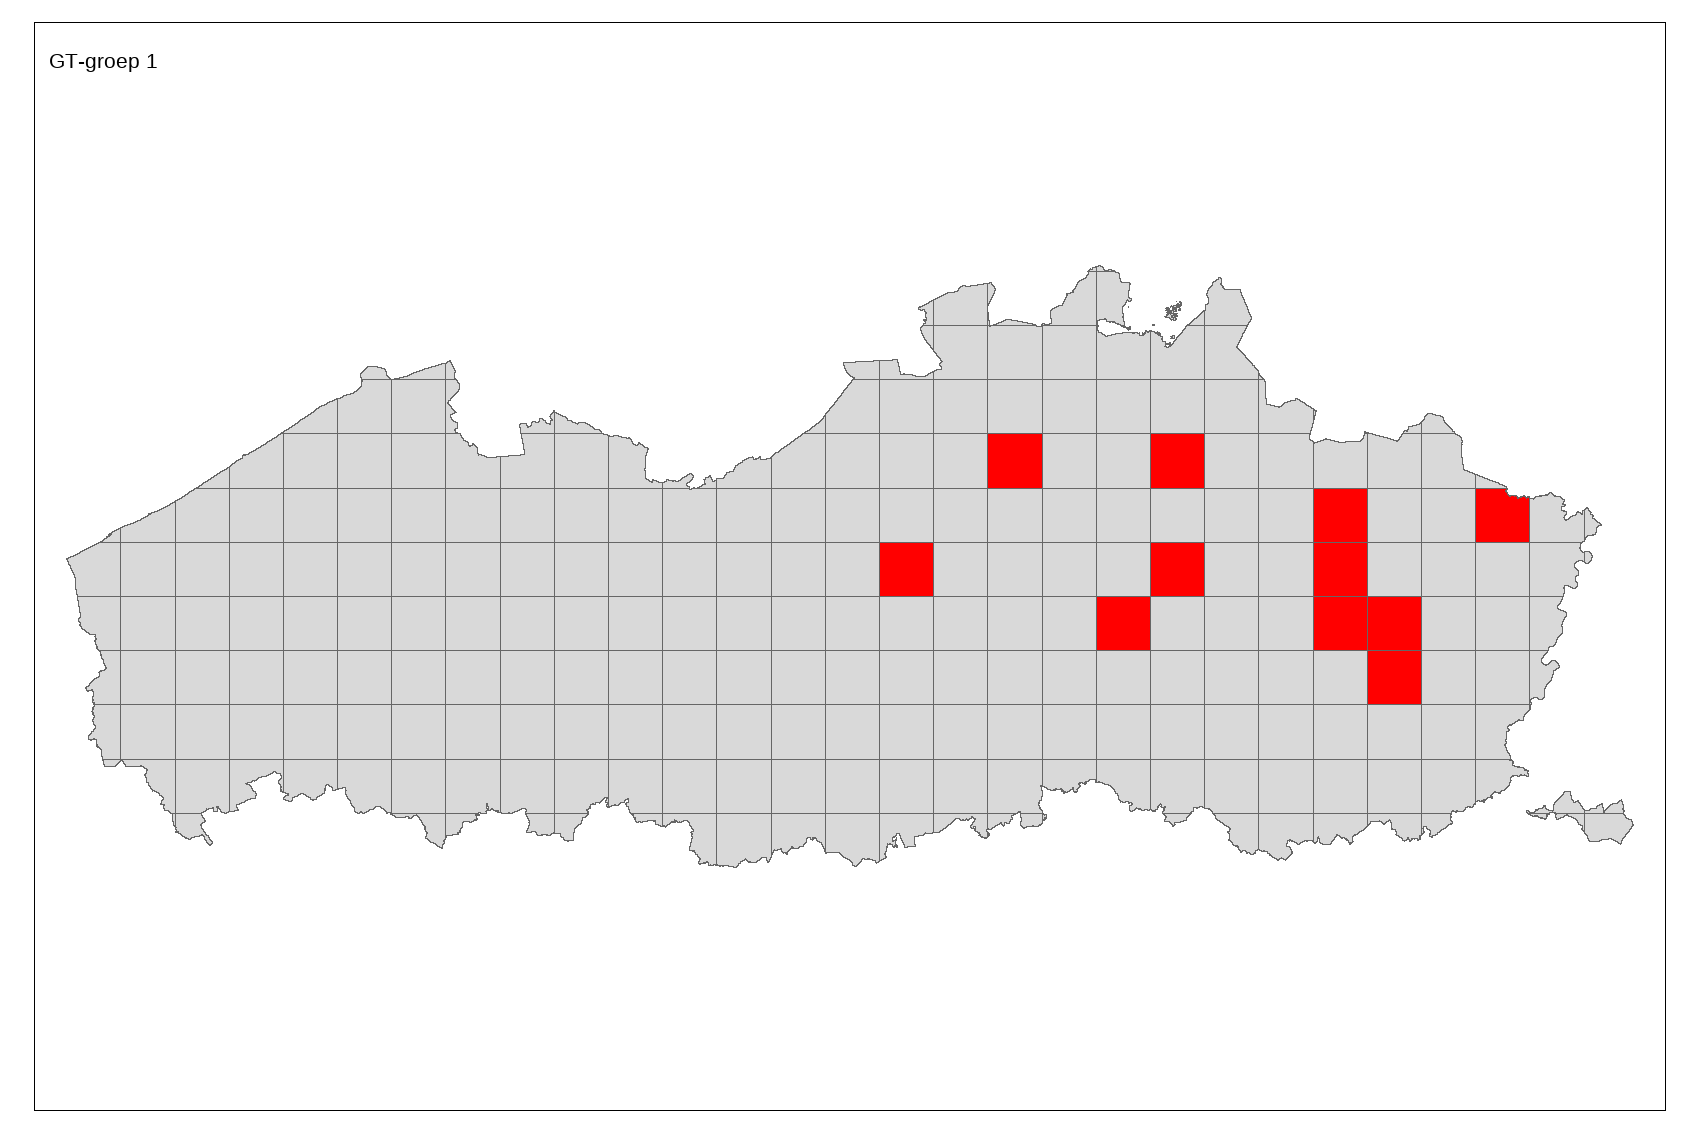
\includegraphics{droogtemeetnet_ontwerp_files/figure-latex/selectie-rastercel-met-meetpunt-fig1-1.pdf}
Figuren \ref{fig:selectie-rastercel-met-meetpunt-fig2},
\ref{fig:selectie-rastercel-met-meetpunt-fig3},
\ref{fig:selectie-rastercel-met-meetpunt-fig4} en
\ref{fig:selectie-rastercel-met-meetpunt-fig5} tonen de selecties voor
de andere GT-groepen. Er zijn nagenoeg steeds 20 rastercellen
geselecteerd. Bij GT-groepen 2 en 3 liggen deze vrij goed verspreid over
Vlaanderen, voor groepen 4 en 5 zien we duidelijk enkele clusters: bij 4
in de leemstreek en bij 5 in de duinen.

\begin{figure}
\centering
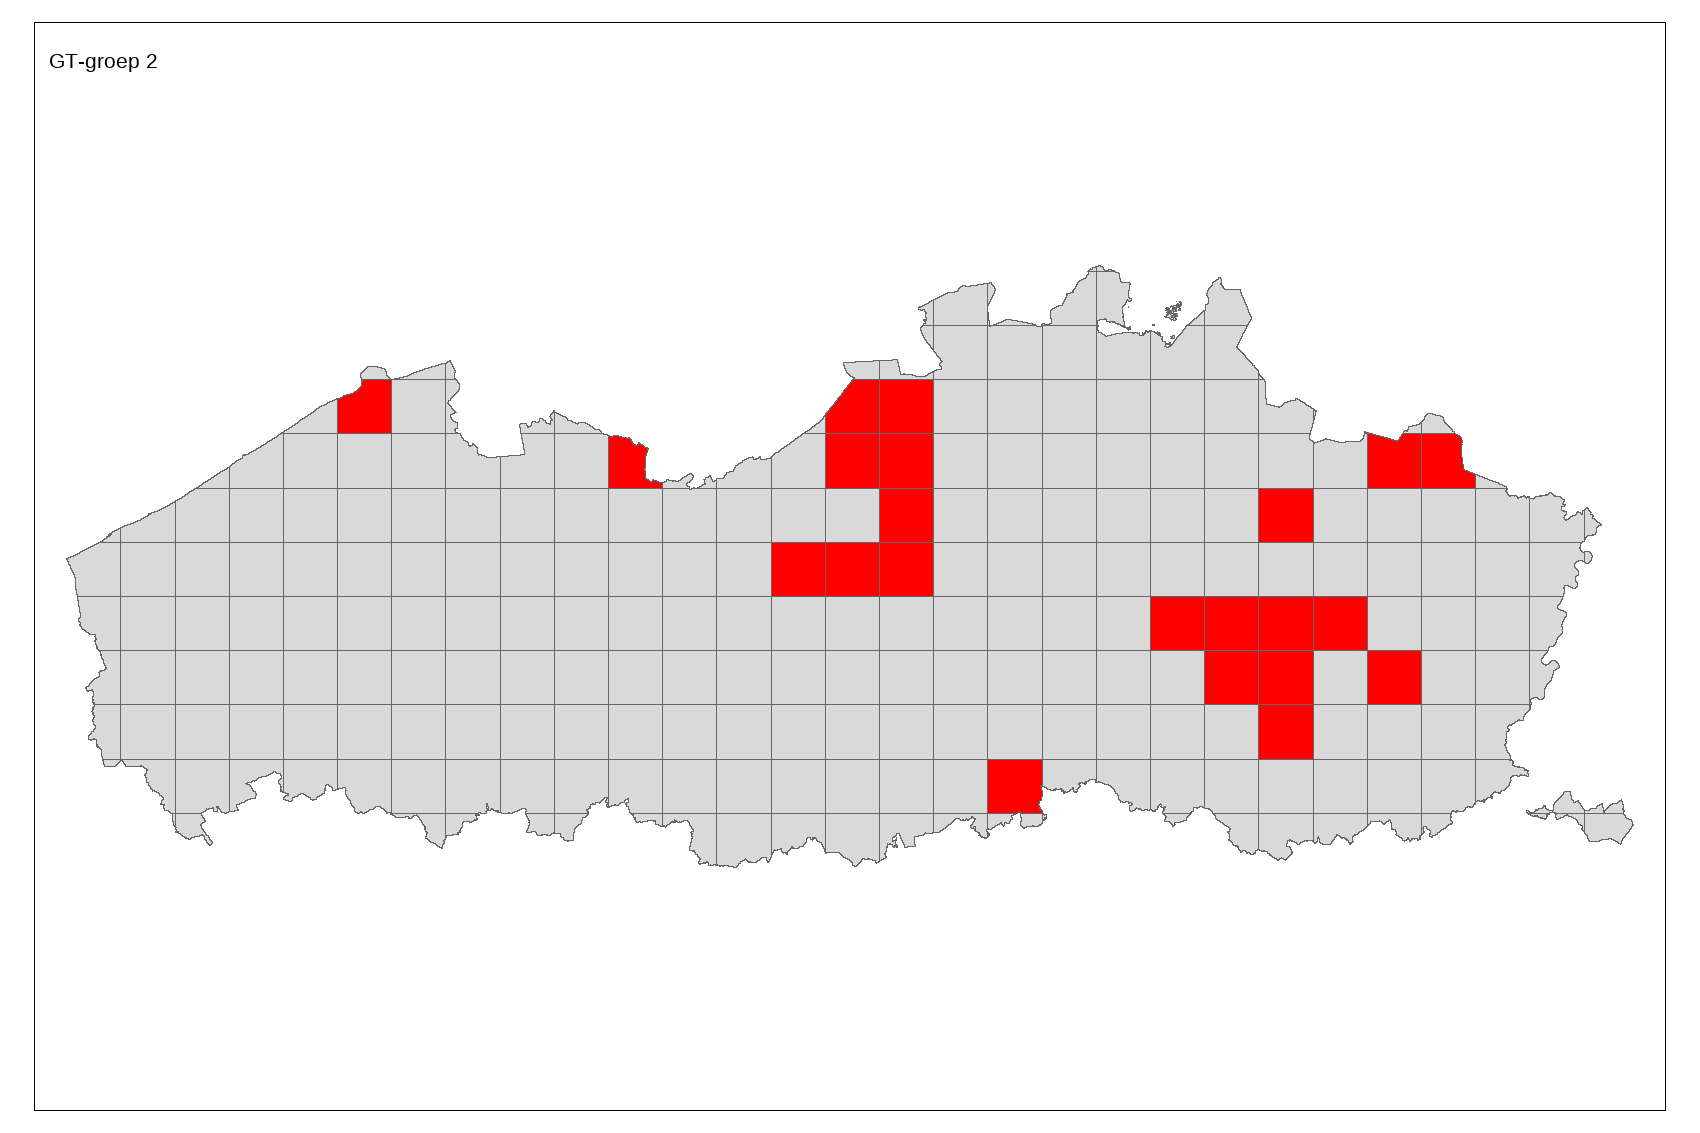
\includegraphics{droogtemeetnet_ontwerp_files/figure-latex/selectie-rastercel-met-meetpunt-fig2-1.pdf}
\caption{\label{fig:selectie-rastercel-met-meetpunt-fig2}Geselecteerde
rastercellen voor GT-groep 2 (= nat)}
\end{figure}

\begin{figure}
\centering
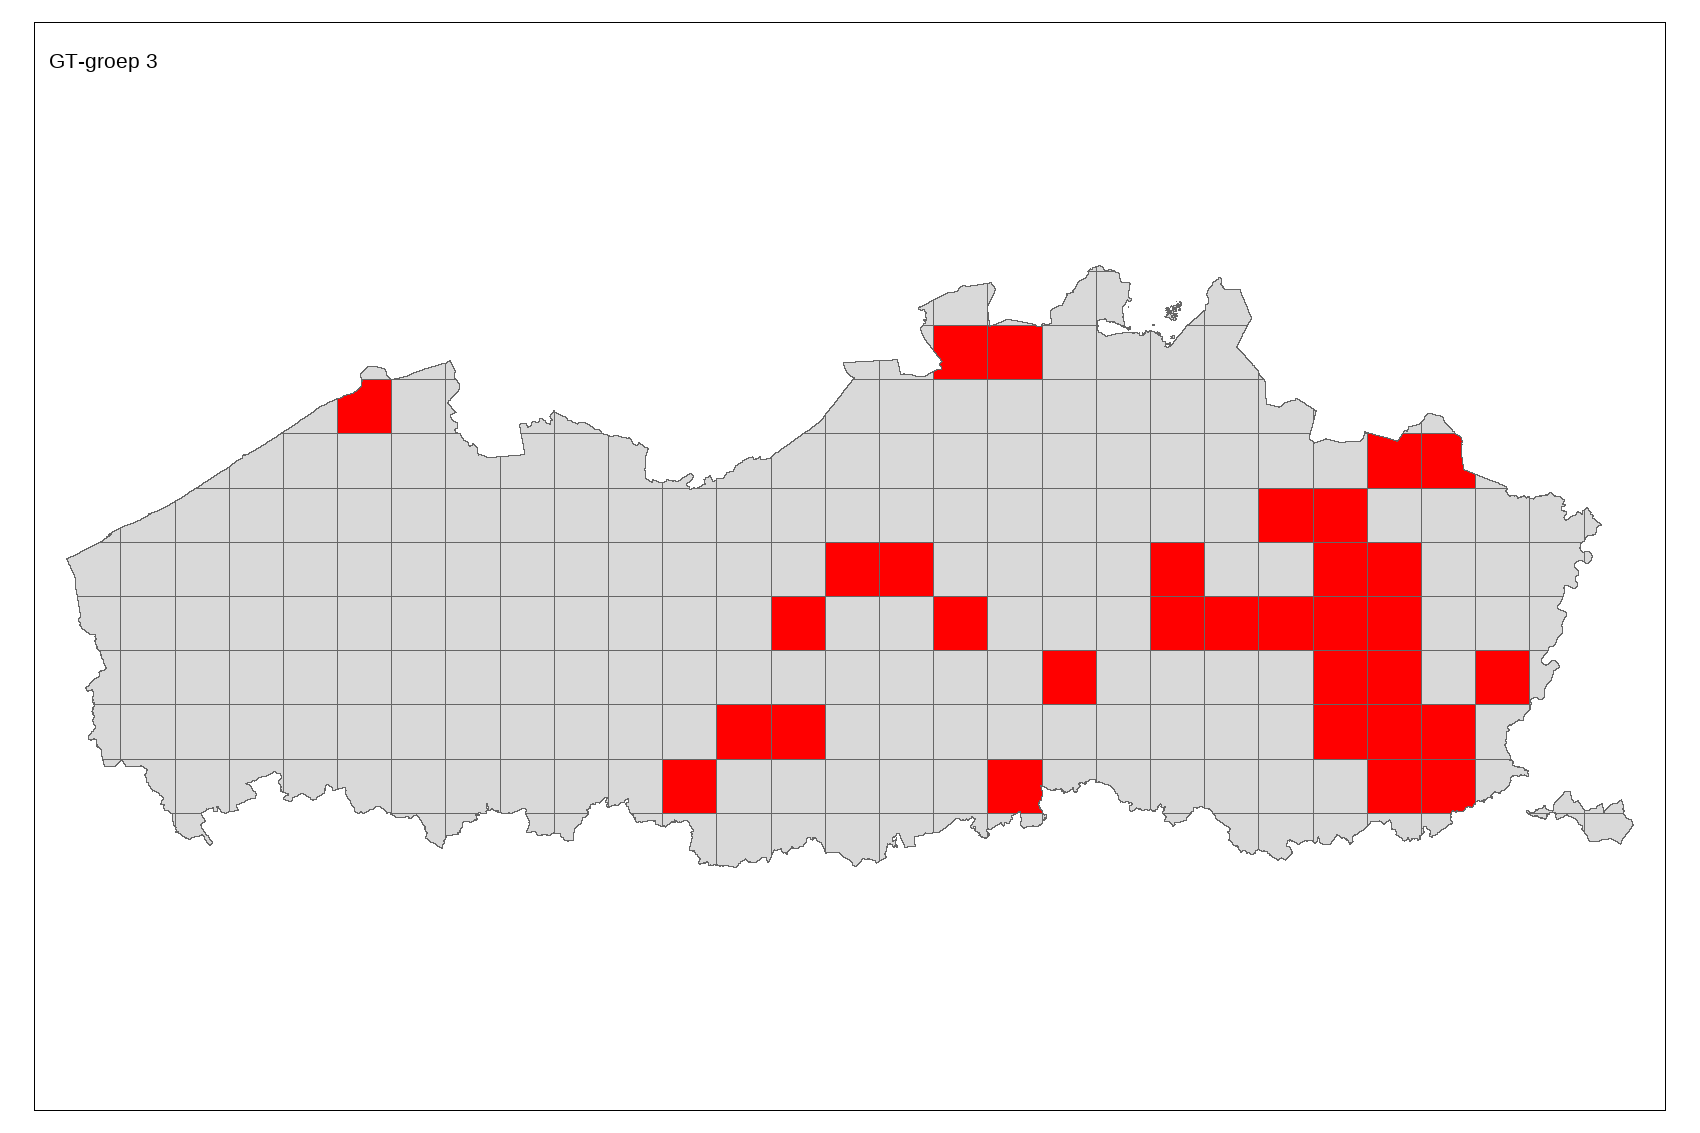
\includegraphics{droogtemeetnet_ontwerp_files/figure-latex/selectie-rastercel-met-meetpunt-fig3-1.pdf}
\caption{\label{fig:selectie-rastercel-met-meetpunt-fig3}Geselecteerde
rastercellen voor GT-groep 3 (= matig nat)}
\end{figure}

\begin{figure}
\centering
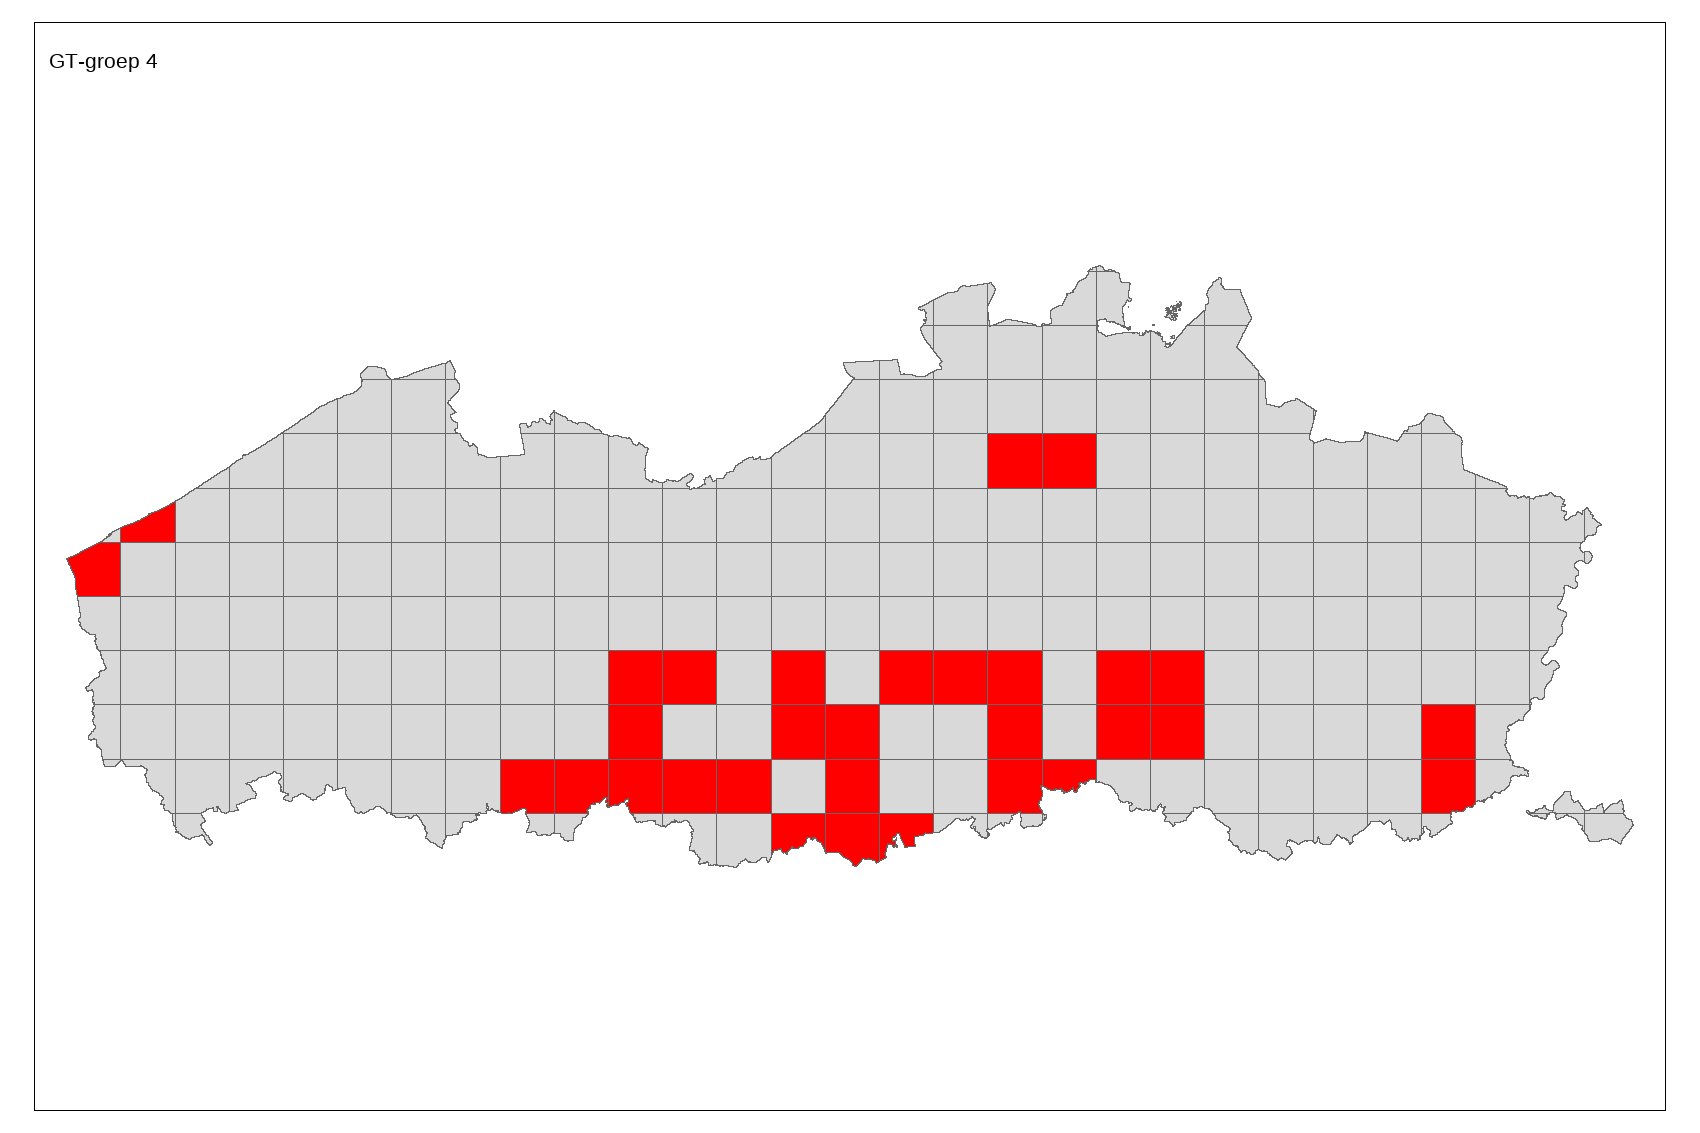
\includegraphics{droogtemeetnet_ontwerp_files/figure-latex/selectie-rastercel-met-meetpunt-fig4-1.pdf}
\caption{\label{fig:selectie-rastercel-met-meetpunt-fig4}Geselecteerde
rastercellen voor GT-groep 4 (= vochtig)}
\end{figure}

\includegraphics{droogtemeetnet_ontwerp_files/figure-latex/selectie-rastercel-met-meetpunt-fig5-1.pdf}
Figuur \ref{fig:selectie-rastercel-met-meetpunt-fig6} geeft het
totaalbeeld.

\begin{figure}
\centering
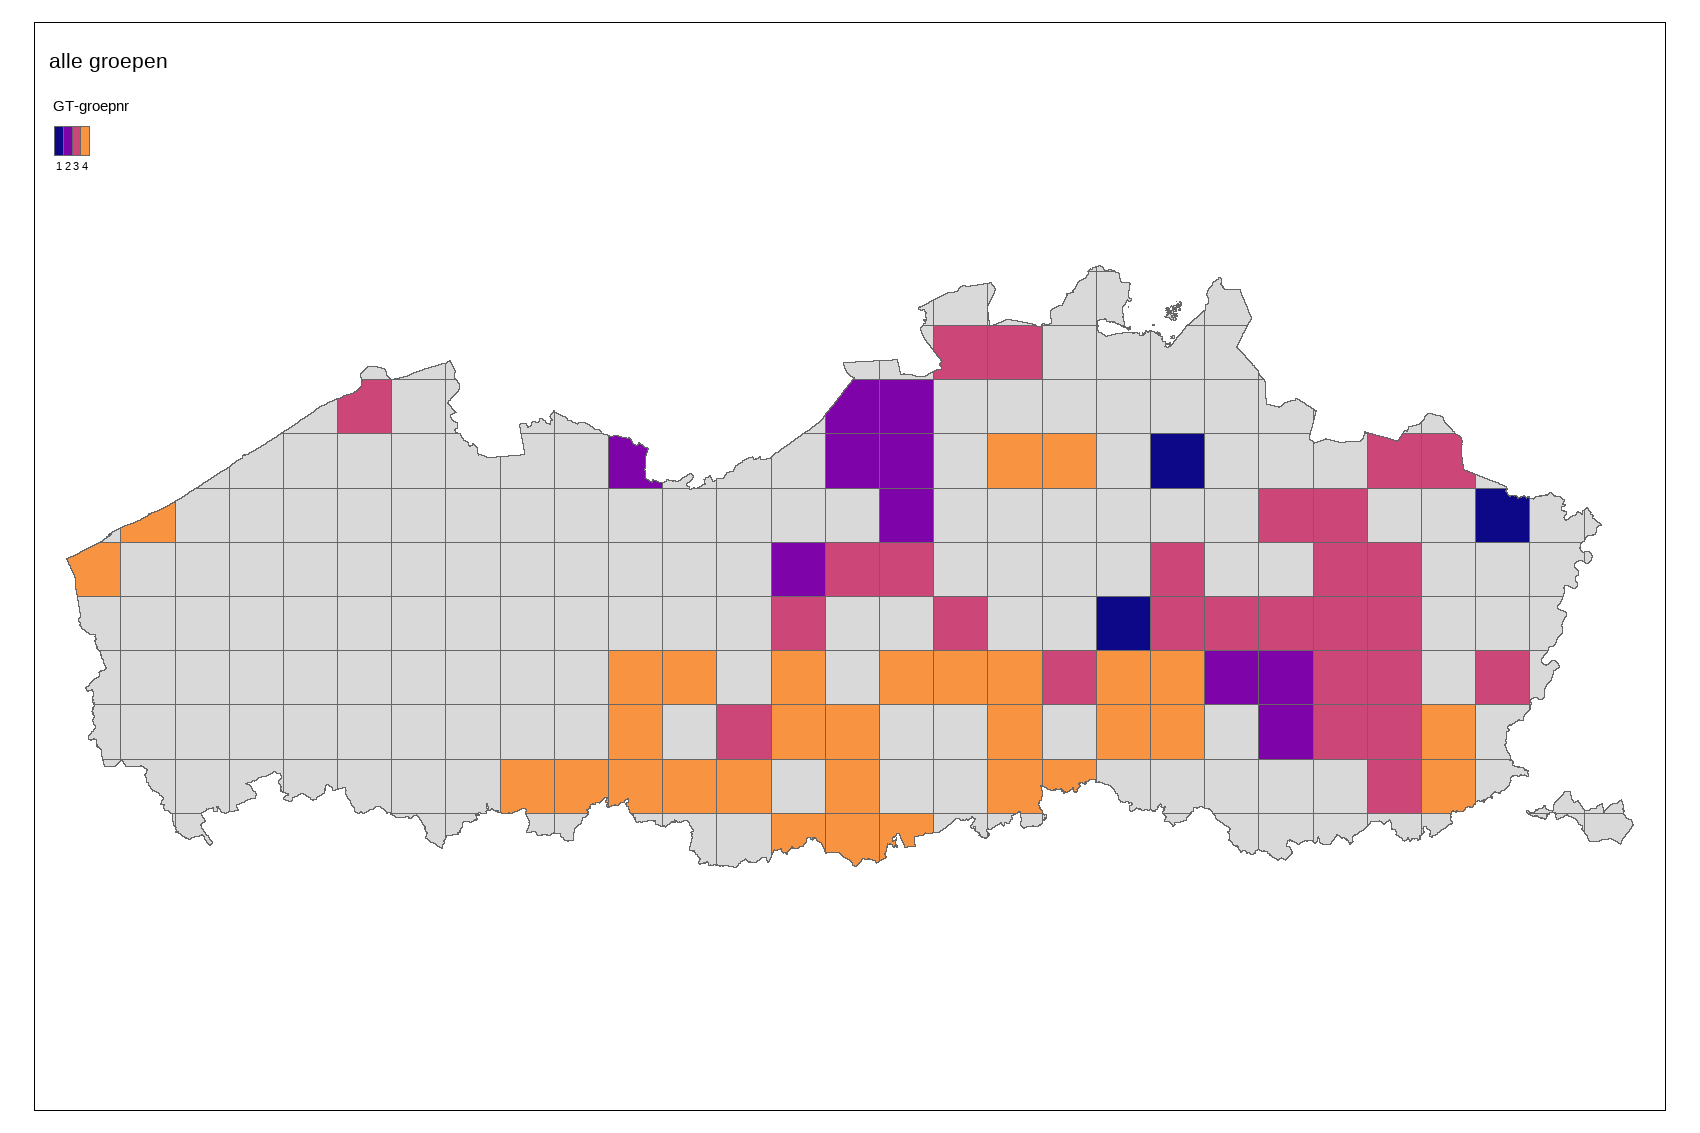
\includegraphics{droogtemeetnet_ontwerp_files/figure-latex/selectie-rastercel-met-meetpunt-fig6-1.pdf}
\caption{\label{fig:selectie-rastercel-met-meetpunt-fig6}Geselecteerde
rastercellen (alle GT-groepen)}
\end{figure}

\section{Selecteren van
grondwater-meetpunten}\label{selecteren-van-grondwater-meetpunten}

Voor deze selectie wordt uitsluitend gewerkt met de Watina-databank. In
het projectvoorstel werden nog andere databanken vermeld:

\begin{enumerate}
\def\labelenumi{\arabic{enumi}.}
\tightlist
\item
  het freatisch grondwatermeetnet van de VMM
\item
  het grondwatermeetnet van het ANB voor beheermonitoring
\end{enumerate}

Het freatisch grondwatermeetnet van de VMM werd al gescreend om te komen
tot het huidige droogtemeetnet. Er kan wel nog nagegaan worden of er in
rastercellen met een tekort aan meetpunten (cat. 1) soms VMM-meetpunten
vallen. \textbf{\emph{eventueel nog te doen}}

Het grondwatermeetnet van ANB is nog in ontwerp. De meetpunten van dit
meetnet zullen ook in de Watina-databank worden opgenomen.

De selectie gebeurde in enkele stappen :

\begin{enumerate}
\def\labelenumi{\arabic{enumi}.}
\tightlist
\item
  Aanduiden van de meetpunten die gelegen zijn in een gaHT.
\item
  Selecteren van de meetpunten die binnen een geselecteerde rastercel
  vallen.
\end{enumerate}

\subsection{Opgave van de meetpunten (Watina-databank) die gelegen zijn
in een verdrogingsgevoelig
type.}\label{opgave-van-de-meetpunten-watina-databank-die-gelegen-zijn-in-een-verdrogingsgevoelig-type.}

Voor deze selectie werd met een zoekstraal van \textbf{3} meter rond een
meetpunt gewerkt. We selecteren enkel de meetpunten die grondwaterpeilen
meten tot op een maximale diepte van 3 m (piëzometer of peilbuis).
Binnen deze straal wordt aangenomen dat het grondwaterregime weinig zal
variëren.

Door het gebruik van een bufferzone en wanneer een peilbuis in een
habitat-complex ligt, kan een peilbuis meerdere keren geselecteerd
worden. Dat kan ertoe leiden dat een rastercel gekozen werd voor een
bep. GT-groep die er in feite maar marginaal aanwezig is. Om dat te
vermijden, voegen we de verschillende habitattypen samen die tot
eenzelfde GT-groep behoren. Alleen de GT-groep met een (gesommeerd)
opp-aandeel van minstens 50\% (in de aan een peilbuis gekoppelde
polygoon) wordt dan weerhouden voor een peilbuis. We selecteren dan de
peilbuizen die met juist één GT-groep kunnen geassocieerd worden.

Tabel \ref{tab:tabel-Watina-in-gaHT} geeft een overzicht van deze 2317
peilbuizen.

\begin{table}

\caption{\label{tab:tabel-Watina-in-gaHT}Watina-meetpunten in een gaHT}
\centering
\begin{tabular}[t]{l|l|r|r|r|r}
\hline
watinacode & gebied & x & y & diepte filter & GT-groep\\
\hline
AABP014 & Aabeek & 178310 & 209590 & 2.740 & 1\\
\hline
AABP017 & Aabeek & 178370 & 209461 & 2.720 & 3\\
\hline
AABP019 & Aabeek & 178417 & 209404 & 2.730 & 3\\
\hline
AABP059 & Aabeek & 177355 & 209634 & 1.450 & 1\\
\hline
AABP060 & Aabeek & 177751 & 209664 & 1.200 & 3\\
\hline
AABP063 & Aabeek & 178910 & 209535 & 1.910 & 3\\
\hline
ABEP011 & Abeek & 230541 & 195642 & 1.340 & 5\\
\hline
ABEP014 & Abeek & 230569 & 195670 & 1.864 & 5\\
\hline
ABEP021 & Abeek & 229808 & 202035 & 1.460 & 2\\
\hline
ABEP022 & Abeek & 229849 & 202009 & 1.670 & 2\\
\hline
ABEP023 & Abeek & 229904 & 201967 & 1.990 & 1\\
\hline
ABEP024 & Abeek & 229859 & 202086 & 1.710 & 2\\
\hline
ABEP031 & Abeek & 230661 & 203698 & 1.850 & 1\\
\hline
ABEP032 & Abeek & 230638 & 203714 & 2.290 & 3\\
\hline
ABEP033 & Abeek & 230608 & 203730 & 1.320 & 3\\
\hline
ABEP034 & Abeek & 230678 & 203741 & 2.110 & 1\\
\hline
ABEP035 & Abeek & 230667 & 203754 & 1.640 & 3\\
\hline
ABEP036 & Abeek & 230650 & 203767 & 2.320 & 3\\
\hline
ABEP037 & Abeek & 230642 & 203779 & 1.310 & 3\\
\hline
ABEP041 & Abeek & 231078 & 204310 & 1.400 & 2\\
\hline
ABEP042 & Abeek & 231054 & 204335 & 1.500 & 3\\
\hline
ABEP043 & Abeek & 231032 & 204357 & 1.360 & 3\\
\hline
ABEP044 & Abeek & 231093 & 204330 & 2.040 & 2\\
\hline
ABEP045 & Abeek & 231081 & 204382 & 2.220 & 3\\
\hline
ABEP046 & Abeek & 231056 & 204396 & 1.570 & 3\\
\hline
ABEP047 & Abeek & 231013 & 204367 & 1.550 & 3\\
\hline
ABEP107 & Abeek & 244825 & 206241 & 1.930 & 3\\
\hline
ABEP108 & Abeek & 244920 & 206371 & 2.850 & 2\\
\hline
ABEP109 & Abeek & 244859 & 206507 & 2.750 & 2\\
\hline
ABEP116 & Abeek & 242112 & 208630 & 2.550 & 5\\
\hline
ABEP119 & Abeek & 240908 & 208538 & 1.100 & 1\\
\hline
ABEP120 & Abeek & 240944 & 208726 & 2.560 & 5\\
\hline
ABEP121 & Abeek & 240946 & 209037 & 2.080 & 1\\
\hline
ABEP122 & Abeek & 240978 & 209184 & 2.650 & 1\\
\hline
ABEP126 & Abeek & 239178 & 208571 & 1.940 & 1\\
\hline
ABEP133 & Abeek & 245756 & 206792 & 2.680 & 2\\
\hline
ALMP001 & Aalmoezenijbos / Aelmoeseneiebos / Gontrodebos & 109770 & 185010 & 1.590 & 4\\
\hline
ALMP002 & Aalmoezenijbos / Aelmoeseneiebos / Gontrodebos & 109744 & 185010 & 1.200 & 4\\
\hline
ALMP003 & Aalmoezenijbos / Aelmoeseneiebos / Gontrodebos & 110287 & 185136 & 0.850 & 4\\
\hline
ARHP009 & Aronst Hoek & 203834 & 177051 & 2.100 & 2\\
\hline
ARHP010 & Aronst Hoek & 203804 & 177070 & 2.300 & 2\\
\hline
ASBP001 & Asbeek & 238494 & 179477 & 0.960 & 1\\
\hline
ASBP003 & Asbeek & 238036 & 179497 & 1.100 & 3\\
\hline
ASHP023 & Achter Schoonhoven & 185344 & 186327 & 1.738 & 3\\
\hline
ASSP005 & Assebroekse meersen & 73910 & 208646 & 1.050 & 3\\
\hline
ASSP006 & Assebroekse meersen & 74033 & 208916 & 1.030 & 3\\
\hline
ASSP009 & Assebroekse meersen & 73613 & 208584 & 1.060 & 3\\
\hline
ASSP010 & Assebroekse meersen & 73583 & 208390 & 1.020 & 3\\
\hline
ASSP012 & Assebroekse meersen & 72225 & 209204 & 1.020 & 3\\
\hline
ASSP014 & Assebroekse meersen & 72187 & 208338 & 2.000 & 4\\
\hline
ASSP105 & Assebroekse meersen & 73910 & 208647 & 2.050 & 3\\
\hline
ASSP106 & Assebroekse meersen & 74033 & 208916 & 2.200 & 3\\
\hline
ASSP109 & Assebroekse meersen & 73613 & 208584 & 2.220 & 3\\
\hline
ASSP110 & Assebroekse meersen & 73583 & 208390 & 2.170 & 3\\
\hline
ASSP112 & Assebroekse meersen & 72157 & 208326 & 1.480 & 4\\
\hline
AVEP007 & Averbode & 194071 & 191836 & 1.980 & 3\\
\hline
AVEP032 & Averbode & 192603 & 192680 & 1.120 & 3\\
\hline
AVEP036 & Averbode & 194308 & 192708 & 2.750 & 3\\
\hline
BARP003 & Berlarebroek & 123702 & 191007 & 1.510 & 3\\
\hline
BARP010 & Berlarebroek & 123418 & 193776 & 1.190 & 1\\
\hline
BARP011 & Berlarebroek & 122829 & 193554 & 1.430 & 1\\
\hline
BARP200 & Berlarebroek & 124175 & 191347 & 2.720 & 3\\
\hline
BARP201 & Berlarebroek & 124175 & 191347 & 0.370 & 3\\
\hline
BASP001 & Bastenakker & 112688 & 187526 & 1.750 & 4\\
\hline
BAVP002 & Bassevillebeek & 51523 & 170489 & 2.290 & 3\\
\hline
BDHP011 & De Haan & 58778 & 220729 & 2.250 & 4\\
\hline
BEBP001 & Bellebeek & 137281 & 173425 & 3.000 & 3\\
\hline
BEBP002 & Bellebeek & 137755 & 173562 & 2.450 & 3\\
\hline
BEBP003 & Bellebeek & 137289 & 173470 & 3.000 & 3\\
\hline
BEBP004 & Bellebeek & 137348 & 173496 & 3.000 & 3\\
\hline
BEBP005 & Bellebeek & 137414 & 173506 & 2.200 & 3\\
\hline
BEBP006 & Bellebeek & 137470 & 173498 & 2.200 & 3\\
\hline
BEBP007 & Bellebeek & 137557 & 173539 & 2.280 & 3\\
\hline
BEBP009 & Bellebeek & 137668 & 173499 & 2.150 & 3\\
\hline
BEBP010 & Bellebeek & 137710 & 173516 & 2.200 & 3\\
\hline
BEBP012 & Bellebeek & 133244 & 174908 & 2.200 & 3\\
\hline
BEBP013 & Bellebeek & 133268 & 174873 & 1.090 & 3\\
\hline
BELP001 & de Belv<e9>d<e8>re & 28357 & 199975 & 2.000 & 4\\
\hline
BELP004 & de Belv<e9>d<e8>re & 28016 & 199778 & 2.470 & 5\\
\hline
BELP005 & de Belv<e9>d<e8>re & 28044 & 199714 & 0.960 & 5\\
\hline
BELP006 & de Belv<e9>d<e8>re & 28068 & 199648 & 0.990 & 5\\
\hline
BELP008 & de Belv<e9>d<e8>re & 28242 & 199806 & 1.900 & 5\\
\hline
BELP009 & de Belv<e9>d<e8>re & 28145 & 199761 & 1.130 & 5\\
\hline
BELP010 & de Belv<e9>d<e8>re & 27947 & 199669 & 1.600 & 5\\
\hline
BELP011 & de Belv<e9>d<e8>re & 28088 & 200085 & 2.350 & 5\\
\hline
BNDP001 & Bunders & 178755 & 195414 & 1.080 & 3\\
\hline
BNDP002 & Bunders & 178702 & 195360 & 1.580 & 3\\
\hline
BNDP003 & Bunders & 178646 & 195252 & 1.840 & 3\\
\hline
BNDP004 & Bunders & 178562 & 195145 & 1.750 & 3\\
\hline
BNDP101 & Bunders & 178755 & 195414 & 1.080 & 3\\
\hline
BNDP104 & Bunders & 178561 & 195145 & 2.900 & 3\\
\hline
BOBP003 & Bosbeekvallei & 235747 & 190459 & 1.170 & 3\\
\hline
BOBP005 & Bosbeekvallei & 236659 & 191978 & 1.630 & 3\\
\hline
BOBP007 & Bosbeekvallei & 236555 & 192260 & 1.000 & 2\\
\hline
BOBP011 & Bosbeekvallei & 236805 & 192610 & 0.810 & 1\\
\hline
BOBP014 & Bosbeekvallei & 239688 & 195995 & 1.670 & 2\\
\hline
BOBP016 & Bosbeekvallei & 239779 & 195779 & 0.980 & 1\\
\hline
BOBP017 & Bosbeekvallei & 239826 & 195698 & 2.250 & 2\\
\hline
BOBP018 & Bosbeekvallei & 240525 & 196690 & 1.310 & 1\\
\hline
BOBP227 & Bosbeekvallei & 234781 & 189289 & 2.880 & 3\\
\hline
BOBP301 & Bosbeekvallei & 239881 & 195909 & 0.500 & 3\\
\hline
BOBP303 & Bosbeekvallei & 239925 & 195868 & 0.500 & 1\\
\hline
BOBP304 & Bosbeekvallei & 239926 & 195869 & 1.500 & 1\\
\hline
BOBP308 & Bosbeekvallei & 236680 & 192008 & 1.500 & 1\\
\hline
BOBP309 & Bosbeekvallei & 236670 & 192023 & 3.000 & 1\\
\hline
BOBP310 & Bosbeekvallei & 236671 & 192024 & 1.500 & 1\\
\hline
BOBP311 & Bosbeekvallei & 236664 & 192031 & 1.500 & 1\\
\hline
BOBP413 & Bosbeekvallei & 237022 & 193010 & 2.310 & 1\\
\hline
BOBP417 & Bosbeekvallei & 233743 & 188975 & 1.570 & 1\\
\hline
BOBP419 & Bosbeekvallei & 233834 & 188826 & 1.710 & 3\\
\hline
BOEP001 & Boembeke & 107447 & 170403 & 2.550 & 3\\
\hline
BOEP003 & Boembeke & 107334 & 170403 & 2.800 & 4\\
\hline
BOKP002 & Bonte Klepper & 174663 & 225091 & 0.910 & 3\\
\hline
BOKP003 & Bonte Klepper & 174616 & 225006 & 1.560 & 3\\
\hline
BOKP004 & Bonte Klepper & 174592 & 225058 & 0.660 & 3\\
\hline
BOKP005 & Bonte Klepper & 174663 & 225091 & 2.280 & 3\\
\hline
BORP001 & Heideveld-Bornebeek & 74758 & 200334 & 1.990 & 4\\
\hline
BORP002 & Heideveld-Bornebeek & 74718 & 200286 & 1.875 & 4\\
\hline
BORP005 & Heideveld-Bornebeek & 74226 & 200692 & 2.200 & 3\\
\hline
BRAP002 & Bos van Ranst & 163992 & 210550 & 0.850 & 4\\
\hline
BRAP003 & Bos van Ranst & 163755 & 210701 & 1.610 & 4\\
\hline
BRAP009 & Bos van Ranst & 165408 & 210432 & 1.210 & 4\\
\hline
BRAP012 & Bos van Ranst & 164256 & 210225 & 1.940 & 1\\
\hline
BRAP013 & Bos van Ranst & 163638 & 209464 & 1.850 & 4\\
\hline
BRAP015 & Bos van Ranst & 164256 & 210225 & 1.880 & 1\\
\hline
BRAP016 & Bos van Ranst & 164272 & 210225 & 2.000 & 1\\
\hline
BRAP017 & Bos van Ranst & 163808 & 209589 & 0.700 & 4\\
\hline
BRAP018 & Bos van Ranst & 163806 & 209584 & 2.710 & 4\\
\hline
BRAP021 & Bos van Ranst & 163821 & 209812 & 1.920 & 4\\
\hline
BRAP022 & Bos van Ranst & 163990 & 209731 & 0.930 & 4\\
\hline
BRAP023 & Bos van Ranst & 164037 & 209830 & 1.370 & 4\\
\hline
BRAP024 & Bos van Ranst & 164180 & 209978 & 0.810 & 4\\
\hline
BRAP033 & Bos van Ranst & 163015 & 209698 & 1.650 & 4\\
\hline
BRAP034 & Bos van Ranst & 163130 & 209787 & 1.770 & 4\\
\hline
BRAP037 & Bos van Ranst & 162923 & 209832 & 1.490 & 4\\
\hline
BRAP102 & Bos van Ranst & 163992 & 210550 & 1.800 & 4\\
\hline
BRAP116 & Bos van Ranst & 164272 & 210225 & 2.240 & 1\\
\hline
BRAP117 & Bos van Ranst & 163808 & 209589 & 1.500 & 4\\
\hline
BRAP122 & Bos van Ranst & 163990 & 209731 & 1.890 & 4\\
\hline
BRAP124 & Bos van Ranst & 164180 & 209978 & 1.670 & 4\\
\hline
BREP007 & Bredene - De Haan & 53451 & 217236 & 2.810 & 4\\
\hline
BREP008 & Bredene - De Haan & 53371 & 217396 & 2.310 & 4\\
\hline
BREP101 & Bredene - De Haan & 49182 & 215192 & 2.960 & 5\\
\hline
BREP106 & Bredene - De Haan & 49317 & 215076 & 2.950 & 5\\
\hline
BREP201 & Bredene - De Haan & 55379 & 218541 & 2.190 & 5\\
\hline
BREP202 & Bredene - De Haan & 55440 & 218464 & 2.910 & 5\\
\hline
BREP203 & Bredene - De Haan & 55243 & 218558 & 2.950 & 5\\
\hline
BREP204 & Bredene - De Haan & 55302 & 218484 & 2.670 & 5\\
\hline
BREP205 & Bredene - De Haan & 55139 & 218468 & 2.550 & 5\\
\hline
BREP206 & Bredene - De Haan & 55099 & 218328 & 2.620 & 5\\
\hline
BREP207 & Bredene - De Haan & 54921 & 218343 & 2.700 & 5\\
\hline
BREP210 & Bredene - De Haan & 55034 & 218027 & 2.800 & 5\\
\hline
BREP216 & Bredene - De Haan & 53973 & 217630 & 2.750 & 5\\
\hline
BRGP025 & Bourgoyen & 100788 & 195262 & 1.540 & 2\\
\hline
BRGP026 & Bourgoyen & 100786 & 195266 & 1.330 & 2\\
\hline
BRGP027 & Bourgoyen & 100782 & 195272 & 1.520 & 2\\
\hline
BRGP028 & Bourgoyen & 100779 & 195280 & 1.510 & 2\\
\hline
BRGP033 & Bourgoyen & 101920 & 194795 & 1.430 & 3\\
\hline
BRGP034 & Bourgoyen & 101918 & 194799 & 1.570 & 3\\
\hline
BRGP035 & Bourgoyen & 101915 & 194804 & 1.560 & 3\\
\hline
BRGP036 & Bourgoyen & 101913 & 194810 & 2.360 & 3\\
\hline
BRSP008 & Domeinbos Brasschaat (Inslag) & 160451 & 222061 & 2.190 & 5\\
\hline
BSBP003 & Blauwschuurbroek & 179601 & 167693 & 0.520 & 3\\
\hline
BTEP003 & Bos 't Ename & 99330 & 172638 & 1.220 & 4\\
\hline
BTEP004 & Bos 't Ename & 99362 & 172612 & 1.300 & 4\\
\hline
BTEP005 & Bos 't Ename & 99388 & 172580 & 1.700 & 4\\
\hline
BTEP006 & Bos 't Ename & 99428 & 172556 & 2.190 & 4\\
\hline
BTEP007 & Bos 't Ename & 99509 & 172634 & 1.450 & 4\\
\hline
BTEP008 & Bos 't Ename & 99517 & 172644 & 1.670 & 4\\
\hline
BTEP009 & Bos 't Ename & 99497 & 172627 & 1.490 & 4\\
\hline
BTEP010 & Bos 't Ename & 99546 & 172536 & 1.790 & 3\\
\hline
BTEP018 & Bos 't Ename & 99370 & 172598 & 2.880 & 4\\
\hline
BTEP020 & Bos 't Ename & 99339 & 172624 & 1.220 & 4\\
\hline
BTEP022 & Bos 't Ename & 99302 & 172656 & 2.820 & 4\\
\hline
BTEP023 & Bos 't Ename & 99282 & 172685 & 2.750 & 4\\
\hline
BTEP034 & Bos 't Ename & 99421 & 172549 & 2.830 & 4\\
\hline
BTEP035 & Bos 't Ename & 99344 & 172614 & 1.270 & 4\\
\hline
BTRP001 & Bos ter Rijst & 101924 & 164018 & 2.170 & 4\\
\hline
BTRP002 & Bos ter Rijst & 101925 & 164003 & 1.210 & 1\\
\hline
BUCP004 & Buckenslinde & 229712 & 170654 & 1.170 & 1\\
\hline
BUCP006 & Buckenslinde & 229917 & 170400 & 1.810 & 2\\
\hline
BUCP008 & Buckenslinde & 229928 & 170390 & 2.810 & 2\\
\hline
BUIP011 & Buitengoor & 206653 & 212113 & 1.540 & 1\\
\hline
BUIP012 & Buitengoor & 206540 & 212103 & 1.500 & 1\\
\hline
BUIP014 & Buitengoor & 206517 & 212120 & 1.810 & 1\\
\hline
BUIP015 & Buitengoor & 206639 & 212165 & 2.000 & 1\\
\hline
BUIP016 & Buitengoor & 206637 & 212165 & 1.500 & 1\\
\hline
BUIP021 & Buitengoor & 206444 & 211899 & 1.140 & 1\\
\hline
BUIP023 & Buitengoor & 206653 & 212114 & 2.330 & 1\\
\hline
BUIP026 & Buitengoor & 206595 & 212157 & 2.400 & 1\\
\hline
BUIP027 & Buitengoor & 206595 & 212155 & 1.390 & 1\\
\hline
BUIP029 & Buitengoor & 206552 & 212168 & 2.400 & 1\\
\hline
BUIP030 & Buitengoor & 206550 & 212169 & 1.500 & 1\\
\hline
BUIP031 & Buitengoor & 206473 & 212059 & 1.660 & 1\\
\hline
BUIP032 & Buitengoor & 206473 & 212059 & 1.300 & 1\\
\hline
BUIP033 & Buitengoor & 206472 & 212059 & 1.800 & 1\\
\hline
BUIP035 & Buitengoor & 206335 & 212060 & 0.402 & 1\\
\hline
BUIP039 & Buitengoor & 206465 & 212275 & 1.180 & 3\\
\hline
BUIP040 & Buitengoor & 205688 & 211963 & 0.800 & 3\\
\hline
BUIP041 & Buitengoor & 205438 & 211876 & 1.100 & 3\\
\hline
BUIP042 & Buitengoor & 205464 & 211483 & 1.030 & 3\\
\hline
BUIP046 & Buitengoor & 206678 & 212320 & 1.790 & 3\\
\hline
BUIP047 & Buitengoor & 206473 & 212155 & 1.720 & 1\\
\hline
BUIP048 & Buitengoor & 206477 & 212094 & 1.690 & 1\\
\hline
BUIP201 & Buitengoor & 206658 & 212170 & 1.500 & 1\\
\hline
BUIP202 & Buitengoor & 206719 & 212176 & 1.020 & 3\\
\hline
BUIP203 & Buitengoor & 206628 & 212162 & 0.700 & 1\\
\hline
BUIP204 & Buitengoor & 206543 & 212111 & 1.395 & 1\\
\hline
BUIP205 & Buitengoor & 206452 & 212085 & 0.930 & 1\\
\hline
BUIP206 & Buitengoor & 206260 & 211815 & 1.380 & 1\\
\hline
BUIP207 & Buitengoor & 206358 & 212049 & 1.460 & 1\\
\hline
BUIP208 & Buitengoor & 206571 & 211925 & 1.470 & 3\\
\hline
BUIP211 & Buitengoor & 206397 & 211943 & 0.870 & 1\\
\hline
BUIP214 & Buitengoor & 206401 & 211881 & 0.700 & 1\\
\hline
BUIP215 & Buitengoor & 206495 & 211904 & 0.590 & 1\\
\hline
BUIP216 & Buitengoor & 206292 & 211741 & 0.640 & 1\\
\hline
BUIP217 & Buitengoor & 206672 & 212266 & 1.470 & 3\\
\hline
BUIP218 & Buitengoor & 206567 & 212273 & 0.950 & 3\\
\hline
BUIP219 & Buitengoor & 206487 & 212247 & 0.640 & 3\\
\hline
BUIP227 & Buitengoor & 206447 & 212197 & 2.970 & 1\\
\hline
BUIP230 & Buitengoor & 206404 & 212112 & 1.470 & 1\\
\hline
BUIP237 & Buitengoor & 206691 & 212071 & 1.130 & 1\\
\hline
BUIP239 & Buitengoor & 206508 & 212285 & 1.460 & 3\\
\hline
BUIP240 & Buitengoor & 206476 & 211847 & 0.860 & 3\\
\hline
BUIP241 & Buitengoor & 206552 & 211872 & 1.100 & 3\\
\hline
BUIP242 & Buitengoor & 206696 & 211999 & 1.470 & 3\\
\hline
BUIP243 & Buitengoor & 206358 & 212049 & 1.340 & 1\\
\hline
BUIP250 & Buitengoor & 206719 & 212176 & 1.480 & 3\\
\hline
BUIP251 & Buitengoor & 206719 & 212176 & 1.460 & 3\\
\hline
BUIP273 & Buitengoor & 206758 & 212118 & 1.160 & 3\\
\hline
BUIP275 & Buitengoor & 206692 & 212113 & 1.480 & 1\\
\hline
BUIP277 & Buitengoor & 206653 & 212113 & 1.470 & 1\\
\hline
BUIP278 & Buitengoor & 206653 & 212113 & 2.990 & 1\\
\hline
BUIP279 & Buitengoor & 206552 & 211872 & 2.970 & 3\\
\hline
BUIP280 & Buitengoor & 206496 & 212004 & 1.030 & 1\\
\hline
BUIP281 & Buitengoor & 206496 & 212004 & 2.520 & 1\\
\hline
BUIP291 & Buitengoor & 206476 & 211847 & 2.950 & 3\\
\hline
BUNP001 & Paddegat-bunkerweiden & 57800 & 216439 & 2.680 & 5\\
\hline
BURP004 & Burreken & 103397 & 166083 & 1.250 & 1\\
\hline
BVBP010 & Bergerven & 242531 & 196429 & 0.870 & 4\\
\hline
CABP303 & Cabourduinen & 23662 & 195978 & 2.125 & 5\\
\hline
CATP001 & Cathille & 58924 & 213475 & 1.040 & 2\\
\hline
CATP002 & Cathille & 58849 & 213505 & 1.460 & 2\\
\hline
CATP004 & Cathille & 58649 & 214127 & 1.220 & 5\\
\hline
CATP101 & Cathille & 58925 & 213474 & 1.080 & 2\\
\hline
COOP001 & Coolhembos & 146113 & 196127 & 1.400 & 1\\
\hline
DAKP001 & Daknamse Meersen & 123404 & 201411 & 1.770 & 3\\
\hline
DAKP002 & Daknamse Meersen & 123432 & 201437 & 1.750 & 3\\
\hline
DBLP001 & De Blankaart & 44425 & 186992 & 1.400 & 3\\
\hline
DBLP003 & De Blankaart & 43710 & 187356 & 2.490 & 2\\
\hline
DBLP004 & De Blankaart & 43715 & 187242 & 1.470 & 3\\
\hline
DBLP006 & De Blankaart & 43929 & 186722 & 1.990 & 3\\
\hline
DBLP007 & De Blankaart & 43892 & 186705 & 1.850 & 3\\
\hline
DBLP008 & De Blankaart & 43891 & 186705 & 1.120 & 3\\
\hline
DBLP011 & De Blankaart & 44086 & 186662 & 1.550 & 2\\
\hline
DBLP012 & De Blankaart & 44095 & 186646 & 1.290 & 2\\
\hline
DBLP106 & De Blankaart & 41207 & 187210 & 2.600 & 4\\
\hline
DBLP119 & De Blankaart & 41299 & 186474 & 2.100 & 4\\
\hline
DBLP122 & De Blankaart & 44164 & 187580 & 2.440 & 2\\
\hline
DBLP123 & De Blankaart & 44043 & 187525 & 1.960 & 4\\
\hline
DBLP124 & De Blankaart & 43564 & 187183 & 1.460 & 2\\
\hline
DBLP125 & De Blankaart & 43602 & 187140 & 1.590 & 2\\
\hline
DBLP126 & De Blankaart & 43654 & 186905 & 2.300 & 4\\
\hline
DBLP128 & De Blankaart & 41239 & 187262 & 2.370 & 4\\
\hline
DBLP129 & De Blankaart & 43475 & 187595 & 1.550 & 4\\
\hline
DEMP007 & de Merode-Herselt & 190806 & 194941 & 2.220 & 1\\
\hline
DEMP011 & de Merode-Herselt & 190657 & 194916 & 2.000 & 1\\
\hline
DHEP004 & D' Heye & 53841 & 216470 & 2.930 & 5\\
\hline
DHEP006 & D' Heye & 53751 & 216157 & 2.520 & 5\\
\hline
DHEP009 & D' Heye & 53894 & 216146 & 2.840 & 5\\
\hline
DHEP012 & D' Heye & 54133 & 216366 & 2.720 & 5\\
\hline
DMLP002 & Dommel & 223774 & 205700 & 2.230 & 3\\
\hline
DMLP003 & Dommel & 223790 & 205684 & 2.650 & 1\\
\hline
DMLP004 & Dommel & 223807 & 205666 & 2.570 & 1\\
\hline
DMLP005 & Dommel & 223817 & 205649 & 2.740 & 1\\
\hline
DMLP006 & Dommel & 223816 & 205650 & 2.170 & 1\\
\hline
DMLP007 & Dommel & 223871 & 205614 & 2.650 & 1\\
\hline
DMLP008 & Dommel & 223892 & 205599 & 2.550 & 1\\
\hline
DMLP009 & Dommel & 223904 & 205592 & 1.820 & 1\\
\hline
DMLP011 & Dommel & 223972 & 205813 & 2.750 & 1\\
\hline
DMLP013 & Dommel & 223999 & 205780 & 2.310 & 1\\
\hline
DMLP014 & Dommel & 224013 & 205766 & 2.720 & 1\\
\hline
DMLP015 & Dommel & 224020 & 205758 & 1.630 & 1\\
\hline
DMLP016 & Dommel & 224590 & 206206 & 1.910 & 1\\
\hline
DMLP019 & Dommel & 224438 & 206281 & 1.840 & 1\\
\hline
DMLP020 & Dommel & 224501 & 206266 & 2.090 & 1\\
\hline
DMLP021 & Dommel & 224557 & 206249 & 2.320 & 1\\
\hline
DMLP023 & Dommel & 224630 & 206197 & 1.520 & 1\\
\hline
DMLP025 & Dommel & 223765 & 205700 & 1.890 & 3\\
\hline
DMLP026 & Dommel & 223881 & 205587 & 2.810 & 1\\
\hline
DMLP029 & Dommel & 224544 & 206253 & 2.210 & 1\\
\hline
DMLP030 & Dommel & 223900 & 205561 & 2.770 & 1\\
\hline
DMLP031 & Dommel & 225481 & 205962 & 1.900 & 2\\
\hline
DMLP032 & Dommel & 225462 & 205953 & 2.000 & 2\\
\hline
DMLP033 & Dommel & 225438 & 205938 & 1.450 & 3\\
\hline
DMLP034 & Dommel & 225413 & 205929 & 1.520 & 3\\
\hline
DMLP035 & Dommel & 224739 & 206745 & 2.320 & 3\\
\hline
DMLP036 & Dommel & 224682 & 206745 & 1.870 & 3\\
\hline
DMLP038 & Dommel & 224569 & 206762 & 1.460 & 3\\
\hline
DMLP039 & Dommel & 223361 & 204761 & 1.845 & 1\\
\hline
DMLP040 & Dommel & 223193 & 204837 & 1.700 & 3\\
\hline
DMLP048 & Dommel & 221815 & 199801 & 1.660 & 3\\
\hline
DMLP049 & Dommel & 221884 & 199884 & 1.050 & 1\\
\hline
DMLP050 & Dommel & 221945 & 199980 & 1.960 & 3\\
\hline
DOBP004 & Kolisheide - dorperloop & 228430 & 211306 & 2.010 & 1\\
\hline
DOEP001 & Doevevallei & 35732 & 164456 & 2.080 & 3\\
\hline
DOEP005 & Doevevallei & 36401 & 164331 & 2.630 & 3\\
\hline
DOEP006 & Doevevallei & 36438 & 164476 & 1.170 & 4\\
\hline
DOEP007 & Doevevallei & 36343 & 164561 & 1.160 & 4\\
\hline
DOMP135 & Dombergheide & 190461 & 227032 & 1.080 & 3\\
\hline
DOMP136 & Dombergheide & 190462 & 227032 & 1.882 & 3\\
\hline
DONP001 & Donkmeer & 122007 & 192333 & 1.928 & 3\\
\hline
DONP002 & Donkmeer & 122095 & 192264 & 1.480 & 3\\
\hline
DONP006 & Donkmeer & 122003 & 192454 & 1.680 & 3\\
\hline
DONP007 & Donkmeer & 121828 & 191432 & 1.490 & 3\\
\hline
DONP009 & Donkmeer & 122693 & 191953 & 1.750 & 1\\
\hline
DORP001 & Dorent & 154260 & 194531 & 0.860 & 3\\
\hline
DORP004 & Dorent & 154347 & 192887 & 1.820 & 3\\
\hline
DORP005 & Dorent & 154407 & 193044 & 1.280 & 3\\
\hline
DORP016 & Dorent & 158521 & 186074 & 1.960 & 3\\
\hline
DORP023 & Dorent & 154284 & 182533 & 1.870 & 3\\
\hline
DORP024 & Dorent & 154823 & 182431 & 2.710 & 4\\
\hline
DPBP006 & Diepenbeek & 222527 & 179904 & 0.000 & 3\\
\hline
DPBP007 & Diepenbeek & 221649 & 179772 & 2.210 & 2\\
\hline
DROP002 & Drongengoed & 85566 & 205542 & 2.110 & 1\\
\hline
DROP003 & Drongengoed & 85655 & 205789 & 1.770 & 1\\
\hline
DULP001 & Duling & 145574 & 156223 & 1.150 & 1\\
\hline
DULP002 & Duling & 145565 & 156231 & 0.870 & 1\\
\hline
DULP003 & Duling & 145553 & 156241 & 1.090 & 1\\
\hline
DUNP001 & Dunbergbroek & 178497 & 180319 & 1.310 & 3\\
\hline
DUNP002 & Dunbergbroek & 178497 & 180319 & 0.710 & 3\\
\hline
DUNP003 & Dunbergbroek & 178516 & 180328 & 1.694 & 3\\
\hline
DUNP004 & Dunbergbroek & 178548 & 180340 & 1.290 & 3\\
\hline
DUNP010 & Dunbergbroek & 178354 & 180655 & 2.060 & 4\\
\hline
DUNP011 & Dunbergbroek & 178562 & 180199 & 1.820 & 4\\
\hline
DUNP012 & Dunbergbroek & 178707 & 179625 & 1.530 & 4\\
\hline
DUNP015 & Dunbergbroek & 178469 & 180313 & 0.740 & 3\\
\hline
DUNP018 & Dunbergbroek & 179028 & 180543 & 1.370 & 3\\
\hline
DURP003 & Durmemeersen & 128298 & 199074 & 1.570 & 3\\
\hline
DURP005 & Durmemeersen & 128264 & 199910 & 1.660 & 3\\
\hline
DURP006 & Durmemeersen & 128191 & 199990 & 1.850 & 3\\
\hline
DURP007 & Durmemeersen & 131419 & 199234 & 1.830 & 3\\
\hline
DURP008 & Durmemeersen & 131410 & 199310 & 1.710 & 3\\
\hline
DURP015 & Durmemeersen & 128773 & 199480 & 2.150 & 3\\
\hline
DURP021 & Durmemeersen & 132182 & 199654 & 1.970 & 3\\
\hline
DYLP002 & Dijlevallei & 169666 & 167242 & 1.270 & 3\\
\hline
DYLP003 & Dijlevallei & 169695 & 167289 & 1.770 & 3\\
\hline
DYLP007 & Dijlevallei & 169592 & 167455 & 2.010 & 3\\
\hline
DYLP008 & Dijlevallei & 169553 & 167729 & 1.410 & 3\\
\hline
DYLP010 & Dijlevallei & 169713 & 167288 & 1.340 & 3\\
\hline
DYLP016 & Dijlevallei & 169553 & 167729 & 2.990 & 3\\
\hline
DYLP018 & Dijlevallei & 169471 & 167314 & 2.180 & 4\\
\hline
DYLP020 & Dijlevallei & 169378 & 167510 & 1.990 & 3\\
\hline
DYLP021 & Dijlevallei & 169440 & 167581 & 2.210 & 3\\
\hline
DYLP022 & Dijlevallei & 169525 & 167847 & 1.930 & 2\\
\hline
DYLP023 & Dijlevallei & 169708 & 167893 & 1.510 & 3\\
\hline
DYLP029 & Dijlevallei & 169238 & 167404 & 1.440 & 2\\
\hline
DYLP030 & Dijlevallei & 169600 & 167277 & 2.090 & 3\\
\hline
DYLP037 & Dijlevallei & 169802 & 167510 & 1.120 & 4\\
\hline
DYLP038 & Dijlevallei & 169834 & 167707 & 1.510 & 4\\
\hline
DYLP039 & Dijlevallei & 169626 & 167500 & 1.390 & 3\\
\hline
DYLP040 & Dijlevallei & 169585 & 167579 & 2.480 & 3\\
\hline
DYLP041 & Dijlevallei & 169604 & 167666 & 1.810 & 3\\
\hline
DYLP042 & Dijlevallei & 169558 & 167907 & 2.280 & 3\\
\hline
DYLP044 & Dijlevallei & 169683 & 167310 & 1.630 & 3\\
\hline
DYLP053 & Dijlevallei & 169768 & 167645 & 1.430 & 2\\
\hline
DYLP055 & Dijlevallei & 169505 & 167935 & 2.150 & 3\\
\hline
DYLP056 & Dijlevallei & 169820 & 167894 & 1.100 & 2\\
\hline
DYLP058 & Dijlevallei & 169641 & 167380 & 2.200 & 3\\
\hline
DYLP059 & Dijlevallei & 169705 & 167400 & 1.760 & 2\\
\hline
DYLP064 & Dijlevallei & 169296 & 166832 & 1.100 & 3\\
\hline
DYLP066 & Dijlevallei & 169359 & 167629 & 2.355 & 3\\
\hline
DYLP070 & Dijlevallei & 169294 & 167490 & 1.790 & 3\\
\hline
DYLP071 & Dijlevallei & 169297 & 167489 & 1.610 & 3\\
\hline
DYLP072 & Dijlevallei & 169307 & 167493 & 1.760 & 3\\
\hline
DYLP073 & Dijlevallei & 169323 & 167496 & 1.760 & 3\\
\hline
DYLP080 & Dijlevallei & 169130 & 167736 & 1.930 & 4\\
\hline
DYLP081 & Dijlevallei & 169188 & 167724 & 2.060 & 3\\
\hline
DYLP082 & Dijlevallei & 169045 & 167592 & 1.800 & 4\\
\hline
DYLP083 & Dijlevallei & 169131 & 167557 & 1.960 & 4\\
\hline
DYLP086 & Dijlevallei & 168957 & 166994 & 1.860 & 4\\
\hline
DYLP087 & Dijlevallei & 169145 & 166917 & 2.110 & 3\\
\hline
DYLP090 & Dijlevallei & 169171 & 167071 & 1.540 & 3\\
\hline
DYLP096 & Dijlevallei & 169526 & 166614 & 2.250 & 3\\
\hline
DYLP098 & Dijlevallei & 168836 & 166696 & 1.100 & 3\\
\hline
DYLP099 & Dijlevallei & 168981 & 166780 & 1.490 & 3\\
\hline
DYLP104 & Dijlevallei & 169342 & 166912 & 1.560 & 3\\
\hline
DYLP108 & Dijlevallei & 169602 & 169321 & 1.920 & 3\\
\hline
DYLP109 & Dijlevallei & 169049 & 168137 & 2.970 & 4\\
\hline
DYLP110 & Dijlevallei & 168864 & 168173 & 2.980 & 4\\
\hline
DYLP112 & Dijlevallei & 169614 & 169718 & 2.240 & 2\\
\hline
DYLP121 & Dijlevallei & 170301 & 170378 & 2.150 & 2\\
\hline
DYLP127 & Dijlevallei & 170625 & 171702 & 2.320 & 1\\
\hline
DYLP128 & Dijlevallei & 171038 & 171936 & 2.140 & 3\\
\hline
DYLP132 & Dijlevallei & 170195 & 171238 & 1.840 & 4\\
\hline
DYLP139 & Dijlevallei & 169209 & 169293 & 2.140 & 4\\
\hline
DYLP154 & Dijlevallei & 169607 & 166997 & 2.490 & 3\\
\hline
DYLP155 & Dijlevallei & 169638 & 166609 & 1.870 & 3\\
\hline
DYLP156 & Dijlevallei & 169478 & 166091 & 1.990 & 3\\
\hline
DYLP157 & Dijlevallei & 169469 & 166259 & 2.000 & 2\\
\hline
DYLP159 & Dijlevallei & 169361 & 168086 & 2.880 & 3\\
\hline
DYLP162 & Dijlevallei & 170716 & 172051 & 2.180 & 4\\
\hline
DYLP168 & Dijlevallei & 171178 & 172123 & 1.880 & 4\\
\hline
DYLP200 & Dijlevallei & 170164 & 171139 & 2.700 & 4\\
\hline
DYLP224 & Dijlevallei & 170317 & 170399 & 1.990 & 2\\
\hline
EENP002 & De Eenbes & 117758 & 204208 & 1.560 & 4\\
\hline
EENP003 & De Eenbes & 117549 & 204202 & 1.550 & 4\\
\hline
EENP016 & De Eenbes & 117759 & 204208 & 1.980 & 4\\
\hline
EENP017 & De Eenbes & 117763 & 204272 & 1.590 & 4\\
\hline
EEUP018 & Eeuwenhout & 37256 & 163444 & 0.800 & 3\\
\hline
EGOP001 & Egoven & 213202 & 160330 & 2.010 & 3\\
\hline
EGOP002 & Egoven & 213233 & 160406 & 2.080 & 2\\
\hline
EKSP028 & Eksterheide & 180226 & 223847 & 2.220 & 5\\
\hline
EKSP029 & Eksterheide & 180237 & 223844 & 2.190 & 5\\
\hline
ELAP002 & De Elsakker & 181162 & 242552 & 2.540 & 2\\
\hline
ELAP009 & De Elsakker & 180348 & 243149 & 2.050 & 1\\
\hline
ELSP003 & Elsbroek & 230624 & 219403 & 1.290 & 3\\
\hline
ELSP004 & Elsbroek & 230639 & 219362 & 1.412 & 3\\
\hline
ELSP005 & Elsbroek & 230715 & 219304 & 1.410 & 3\\
\hline
ELSP006 & Elsbroek & 230796 & 219333 & 1.340 & 3\\
\hline
FBOP002 & Fondatie van Boudelo & 125917 & 207897 & 1.090 & 3\\
\hline
FBOP004 & Fondatie van Boudelo & 124884 & 207274 & 1.370 & 3\\
\hline
FLOP004 & Vijvers van Florival & 169013 & 161968 & 1.400 & 2\\
\hline
FLOP009 & Vijvers van Florival & 169482 & 161118 & 2.500 & 2\\
\hline
GBBP002 & Groeneburgbos & 49224 & 169169 & 1.585 & 4\\
\hline
GNKP007 & Mondingsgebied Grote Nete & 167282 & 202223 & 1.500 & 2\\
\hline
GOBP001 & Gorenbroek & 201583 & 184611 & 1.980 & 3\\
\hline
GOBP002 & Gorenbroek & 201744 & 184514 & 1.360 & 3\\
\hline
GOBP004 & Gorenbroek & 201885 & 184397 & 2.260 & 2\\
\hline
GOOP011 & Het Goor & 185313 & 194925 & 2.710 & 3\\
\hline
GOOP017 & Het Goor & 184742 & 194312 & 2.630 & 3\\
\hline
GOOP019 & Het Goor & 184647 & 194433 & 2.790 & 3\\
\hline
GROP001 & Grotenhoutbos & 187160 & 220275 & 1.710 & 5\\
\hline
GROP002 & Grotenhoutbos & 187160 & 220370 & 1.980 & 5\\
\hline
GROP016 & Grotenhoutbos & 185134 & 220054 & 1.410 & 5\\
\hline
GROP017 & Grotenhoutbos & 185118 & 220056 & 1.610 & 5\\
\hline
GROP019 & Grotenhoutbos & 184965 & 219932 & 1.400 & 5\\
\hline
GROP031 & Grotenhoutbos & 185350 & 219356 & 1.350 & 4\\
\hline
GRSP002 & Griesbroek & 203776 & 204506 & 2.110 & 1\\
\hline
GRSP003 & Griesbroek & 203794 & 204483 & 1.060 & 3\\
\hline
GRSP004 & Griesbroek & 203830 & 204305 & 1.460 & 3\\
\hline
GRSP005 & Griesbroek & 203821 & 204135 & 1.140 & 3\\
\hline
GRYP001 & Grijpenveld (= Aardgat) & 188285 & 167096 & 1.085 & 3\\
\hline
GRYP002 & Grijpenveld (= Aardgat) & 188307 & 167120 & 0.620 & 3\\
\hline
GRYP004 & Grijpenveld (= Aardgat) & 188334 & 167148 & 1.100 & 3\\
\hline
GRYP006 & Grijpenveld (= Aardgat) & 188296 & 167169 & 1.700 & 3\\
\hline
GRYP007 & Grijpenveld (= Aardgat) & 188276 & 167149 & 1.500 & 3\\
\hline
GRYP008 & Grijpenveld (= Aardgat) & 188258 & 167126 & 1.530 & 3\\
\hline
GRYP009 & Grijpenveld (= Aardgat) & 188278 & 167108 & 1.310 & 3\\
\hline
GRYP010 & Grijpenveld (= Aardgat) & 188293 & 167143 & 1.230 & 3\\
\hline
GRYP011 & Grijpenveld (= Aardgat) & 188317 & 167154 & 0.210 & 3\\
\hline
GRYP014 & Grijpenveld (= Aardgat) & 188361 & 167063 & 1.490 & 3\\
\hline
GRYP015 & Grijpenveld (= Aardgat) & 188383 & 167026 & 1.230 & 3\\
\hline
GSCP001 & Groot Schietveld & 167638 & 229848 & 2.300 & 3\\
\hline
GSCP002 & Groot Schietveld & 167621 & 229841 & 1.980 & 3\\
\hline
GSCP003 & Groot Schietveld & 167616 & 229839 & 2.550 & 3\\
\hline
GSCP004 & Groot Schietveld & 167595 & 229834 & 1.880 & 5\\
\hline
GSCP005 & Groot Schietveld & 167586 & 229836 & 2.190 & 5\\
\hline
GSCP006 & Groot Schietveld & 167534 & 229824 & 2.100 & 3\\
\hline
GSCP007 & Groot Schietveld & 167540 & 229836 & 2.120 & 3\\
\hline
GSCP008 & Groot Schietveld & 167490 & 229826 & 2.470 & 3\\
\hline
GSCP009 & Groot Schietveld & 167459 & 229809 & 1.700 & 3\\
\hline
GSCP010 & Groot Schietveld & 167656 & 229861 & 2.270 & 3\\
\hline
GSCP011 & Groot Schietveld & 167660 & 229863 & 2.200 & 3\\
\hline
GSCP012 & Groot Schietveld & 167675 & 229876 & 2.110 & 3\\
\hline
GSCP017 & Groot Schietveld & 167657 & 229201 & 1.910 & 3\\
\hline
GSCP018 & Groot Schietveld & 167646 & 229194 & 2.080 & 3\\
\hline
GSCP019 & Groot Schietveld & 167677 & 229190 & 2.200 & 3\\
\hline
GSCP020 & Groot Schietveld & 167682 & 229188 & 2.480 & 3\\
\hline
GSCP021 & Groot Schietveld & 167691 & 229182 & 1.920 & 3\\
\hline
GSCP024 & Groot Schietveld & 168020 & 229769 & 1.930 & 3\\
\hline
GSCP028 & Groot Schietveld & 165098 & 226891 & 1.074 & 1\\
\hline
GSCP031 & Groot Schietveld & 165207 & 226878 & 1.291 & 1\\
\hline
GSCP032 & Groot Schietveld & 165206 & 226878 & 1.065 & 1\\
\hline
GSCP033 & Groot Schietveld & 165205 & 226900 & 1.020 & 1\\
\hline
GSCP034 & Groot Schietveld & 165256 & 226975 & 1.220 & 3\\
\hline
GSCP035 & Groot Schietveld & 165244 & 226881 & 0.850 & 3\\
\hline
GSCP036 & Groot Schietveld & 165301 & 226908 & 0.900 & 1\\
\hline
GSCP037 & Groot Schietveld & 165191 & 226794 & 1.512 & 1\\
\hline
GSCP038 & Groot Schietveld & 165190 & 226794 & 0.660 & 1\\
\hline
GSCP039 & Groot Schietveld & 165195 & 226726 & 1.290 & 3\\
\hline
GSCP041 & Groot Schietveld & 165152 & 226861 & 0.643 & 1\\
\hline
GSCP042 & Groot Schietveld & 165107 & 228843 & 2.039 & 3\\
\hline
GSCP044 & Groot Schietveld & 165177 & 229023 & 1.440 & 1\\
\hline
GSCP045 & Groot Schietveld & 165054 & 228921 & 0.947 & 1\\
\hline
GSCP048 & Groot Schietveld & 165062 & 228899 & 1.051 & 1\\
\hline
GSCP049 & Groot Schietveld & 165085 & 228917 & 1.210 & 1\\
\hline
GSCP050 & Groot Schietveld & 165107 & 228842 & 1.483 & 3\\
\hline
GSCP058 & Groot Schietveld & 167637 & 229383 & 1.420 & 1\\
\hline
GSCP068 & Groot Schietveld & 165075 & 228761 & 0.920 & 3\\
\hline
GSCP141 & Groot Schietveld & 165151 & 226862 & 0.820 & 1\\
\hline
GSCP145 & Groot Schietveld & 165055 & 228919 & 1.230 & 1\\
\hline
GSCP168 & Groot Schietveld & 165075 & 228761 & 2.670 & 3\\
\hline
GUPP001 & Gulke Putten & 78136 & 197314 & 1.100 & 3\\
\hline
GUPP005 & Gulke Putten & 78178 & 197299 & 0.870 & 3\\
\hline
GUPP007 & Gulke Putten & 78188 & 197254 & 1.035 & 3\\
\hline
GUPP010 & Gulke Putten & 78196 & 197331 & 1.120 & 3\\
\hline
GUPP014 & Gulke Putten & 78199 & 197378 & 1.295 & 3\\
\hline
GUPP015 & Gulke Putten & 78214 & 197358 & 1.160 & 3\\
\hline
GUPP021 & Gulke Putten & 78136 & 197314 & 0.550 & 3\\
\hline
GUPP025 & Gulke Putten & 78179 & 197300 & 0.565 & 3\\
\hline
GUPP034 & Gulke Putten & 78199 & 197378 & 0.560 & 3\\
\hline
GUPP035 & Gulke Putten & 78214 & 197358 & 0.530 & 3\\
\hline
GUPP041 & Gulke Putten & 78176 & 197348 & 1.784 & 3\\
\hline
GUPP044 & Gulke Putten & 78174 & 197346 & 1.210 & 3\\
\hline
HAGP012 & Hageven & 224142 & 218611 & 2.250 & 1\\
\hline
HAGP019 & Hageven & 224064 & 217725 & 2.061 & 2\\
\hline
HAGP023 & Hageven & 222955 & 217220 & 2.020 & 3\\
\hline
HAGP038 & Hageven & 223537 & 217590 & 1.356 & 3\\
\hline
HAGP039 & Hageven & 224384 & 218783 & 2.100 & 2\\
\hline
HAGP073 & Hageven & 222789 & 216198 & 1.730 & 2\\
\hline
HAGP076 & Hageven & 223030 & 216871 & 1.930 & 3\\
\hline
HAGP077 & Hageven & 223081 & 216846 & 2.000 & 3\\
\hline
HAGP100 & Hageven & 222955 & 217220 & 1.716 & 3\\
\hline
HAGP101 & Hageven & 223787 & 217925 & 1.630 & 3\\
\hline
HALP001 & Hallerbos & 143431 & 155389 & 2.020 & 4\\
\hline
HALP002 & Hallerbos & 143429 & 155341 & 1.790 & 4\\
\hline
HALP005 & Hallerbos & 144281 & 156162 & 1.960 & 4\\
\hline
HAYP001 & Hayesbos & 107209 & 163506 & 1.870 & 4\\
\hline
HAYP003 & Hayesbos & 107042 & 163646 & 1.830 & 1\\
\hline
HAYP004 & Hayesbos & 107023 & 163308 & 0.970 & 1\\
\hline
HAYP005 & Hayesbos & 106928 & 162993 & 1.000 & 1\\
\hline
HAZP002 & Handzame & 53706 & 191400 & 0.730 & 4\\
\hline
HAZP003 & Handzame & 53712 & 191363 & 2.715 & 4\\
\hline
HAZP006 & Handzame & 53717 & 191330 & 2.900 & 4\\
\hline
HBTP007 & Helderbeekvallei Terril & 212987 & 193133 & 1.760 & 3\\
\hline
HBTP008 & Helderbeekvallei Terril & 212972 & 193186 & 0.550 & 3\\
\hline
HDPP014 & Hoogdonk Pikhaken & 165046 & 187145 & 2.840 & 4\\
\hline
HDPP015 & Hoogdonk Pikhaken & 164378 & 187248 & 2.720 & 4\\
\hline
HDPP016 & Hoogdonk Pikhaken & 164382 & 187304 & 2.250 & 4\\
\hline
HEIP005 & Heist & 70784 & 226290 & 2.170 & 5\\
\hline
HELP001 & Hellegat  incl. Broekelzen - Rode berg & 37164 & 166283 & 1.120 & 3\\
\hline
HELP005 & Hellegat  incl. Broekelzen - Rode berg & 36206 & 165688 & 1.330 & 4\\
\hline
HELP015 & Hellegat  incl. Broekelzen - Rode berg & 37209 & 165680 & 0.360 & 4\\
\hline
HELP016 & Hellegat  incl. Broekelzen - Rode berg & 36760 & 165511 & 0.995 & 1\\
\hline
HELP017 & Hellegat  incl. Broekelzen - Rode berg & 36500 & 165248 & 1.175 & 4\\
\hline
HELP018 & Hellegat  incl. Broekelzen - Rode berg & 35365 & 165268 & 1.030 & 4\\
\hline
HELP019 & Hellegat  incl. Broekelzen - Rode berg & 36278 & 165652 & 0.920 & 4\\
\hline
HEMP001 & Heverleebos \& Meerdaalbos & 170255 & 165889 & 0.980 & 4\\
\hline
HEMP002 & Heverleebos \& Meerdaalbos & 170255 & 165889 & 1.720 & 4\\
\hline
HEMP003 & Heverleebos \& Meerdaalbos & 170255 & 165889 & 0.980 & 4\\
\hline
HEMP004 & Heverleebos \& Meerdaalbos & 175255 & 165889 & 2.180 & 4\\
\hline
HENP001 & Hengelhoef & 227685 & 190121 & 2.360 & 3\\
\hline
HENP006 & Hengelhoef & 227415 & 190016 & 2.400 & 3\\
\hline
HEUP001 & Heusden LO & 109320 & 190290 & 1.140 & 3\\
\hline
HHUP068 & Houthulst & 50441 & 184533 & 1.120 & 4\\
\hline
HHUP069 & Houthulst & 50397 & 184611 & 1.148 & 4\\
\hline
HIPP003 & Hingense polders & 142098 & 200326 & 2.550 & 3\\
\hline
HIPP004 & Hingense polders & 142171 & 200253 & 2.710 & 3\\
\hline
HIPP005 & Hingense polders & 142275 & 200052 & 2.200 & 3\\
\hline
HIPP008 & Hingense polders & 143006 & 200372 & 2.620 & 3\\
\hline
HIPP009 & Hingense polders & 143054 & 200215 & 2.600 & 3\\
\hline
HIPP011 & Hingense polders & 143593 & 200953 & 2.840 & 3\\
\hline
HIPP012 & Hingense polders & 143650 & 200788 & 2.640 & 3\\
\hline
HIPP015 & Hingense polders & 144325 & 201199 & 2.600 & 3\\
\hline
HIPP016 & Hingense polders & 144362 & 201030 & 2.000 & 3\\
\hline
HIPP021 & Hingense polders & 144238 & 200533 & 2.520 & 3\\
\hline
HLAP002 & Hof van Lachenen & 162340 & 200716 & 1.350 & 2\\
\hline
HOBP014 & Heist op den Berg - Grote Nete & 175162 & 201175 & 2.500 & 3\\
\hline
HOBP015 & Heist op den Berg - Grote Nete & 175154 & 201193 & 2.500 & 3\\
\hline
HOBP016 & Heist op den Berg - Grote Nete & 175140 & 201232 & 2.500 & 3\\
\hline
HOBP017 & Heist op den Berg - Grote Nete & 175116 & 201300 & 2.500 & 3\\
\hline
HOEP003 & Wachtbekken Hoeleden & 195297 & 175381 & 2.300 & 4\\
\hline
HOEP010 & Wachtbekken Hoeleden & 195060 & 174936 & 1.540 & 4\\
\hline
HOEP012 & Wachtbekken Hoeleden & 195299 & 175144 & 2.500 & 4\\
\hline
HOEP017 & Wachtbekken Hoeleden & 195832 & 175522 & 0.630 & 2\\
\hline
HOEP018 & Wachtbekken Hoeleden & 195744 & 175436 & 1.900 & 2\\
\hline
HOEP024 & Wachtbekken Hoeleden & 195665 & 175252 & 1.204 & 2\\
\hline
HOEP025 & Wachtbekken Hoeleden & 195599 & 175180 & 1.050 & 3\\
\hline
HOEP036 & Wachtbekken Hoeleden & 195552 & 175232 & 2.313 & 3\\
\hline
HOEP037 & Wachtbekken Hoeleden & 195364 & 175088 & 1.520 & 3\\
\hline
HOEP063 & Wachtbekken Hoeleden & 194957 & 174596 & 2.300 & 3\\
\hline
HOEP081 & Wachtbekken Hoeleden & 194908 & 174821 & 1.070 & 2\\
\hline
HOEP092 & Wachtbekken Hoeleden & 195755 & 175713 & 1.540 & 2\\
\hline
HOEP094 & Wachtbekken Hoeleden & 195848 & 175310 & 0.720 & 2\\
\hline
HOEP103 & Wachtbekken Hoeleden & 195326 & 175135 & 1.933 & 4\\
\hline
HONP009 & Honegem & 124199 & 182836 & 2.890 & 4\\
\hline
HONP010 & Honegem & 124109 & 183011 & 2.450 & 3\\
\hline
HOPP004 & Hobokense Polder & 148237 & 208881 & 2.290 & 2\\
\hline
HOPP008 & Hobokense Polder & 148749 & 208886 & 2.390 & 3\\
\hline
HOPP009 & Hobokense Polder & 148809 & 208881 & 2.000 & 3\\
\hline
HOSP017 & Houtsaegerduinen/oosthoek & 26564 & 201197 & 2.260 & 4\\
\hline
HOSP018 & Houtsaegerduinen/oosthoek & 26683 & 200875 & 2.940 & 4\\
\hline
HOSP021 & Houtsaegerduinen/oosthoek & 26432 & 200639 & 2.970 & 4\\
\hline
HOSP025 & Houtsaegerduinen/oosthoek & 26022 & 200670 & 2.280 & 4\\
\hline
HOSP026 & Houtsaegerduinen/oosthoek & 25945 & 200361 & 1.910 & 4\\
\hline
HOSP041 & Houtsaegerduinen/oosthoek & 26995 & 199413 & 2.540 & 5\\
\hline
HOSP051 & Houtsaegerduinen/oosthoek & 25960 & 199281 & 2.680 & 4\\
\hline
HOSP055 & Houtsaegerduinen/oosthoek & 26198 & 199550 & 2.050 & 4\\
\hline
HOSP056 & Houtsaegerduinen/oosthoek & 26418 & 199310 & 1.420 & 4\\
\hline
HOSP057 & Houtsaegerduinen/oosthoek & 26628 & 199414 & 1.740 & 4\\
\hline
HOSP058 & Houtsaegerduinen/oosthoek & 26795 & 199501 & 2.600 & 5\\
\hline
HOSP088 & Houtsaegerduinen/oosthoek & 26803 & 199522 & 2.500 & 5\\
\hline
HOSP359 & Houtsaegerduinen/oosthoek & 26995 & 199412 & 2.380 & 5\\
\hline
HRIP001 & Hoge Rielen & 189161 & 214800 & 2.850 & 3\\
\hline
HRIP002 & Hoge Rielen & 189157 & 214802 & 1.470 & 3\\
\hline
HRIP003 & Hoge Rielen & 189153 & 214802 & 0.495 & 3\\
\hline
HRIP004 & Hoge Rielen & 188783 & 214950 & 1.940 & 3\\
\hline
HRIP005 & Hoge Rielen & 188783 & 214949 & 0.540 & 3\\
\hline
IJSP003 & Ijsevallei & 163141 & 164523 & 0.980 & 3\\
\hline
IJSP008 & Ijsevallei & 153888 & 161311 & 2.050 & 1\\
\hline
IJSP009 & Ijsevallei & 153699 & 161428 & 1.500 & 1\\
\hline
IJSP010 & Ijsevallei & 153769 & 161749 & 2.590 & 4\\
\hline
IJSP011 & Ijsevallei & 165317 & 164191 & 2.770 & 3\\
\hline
IJSP017 & Ijsevallei & 165468 & 164008 & 0.650 & 2\\
\hline
IJSP018 & Ijsevallei & 166990 & 166250 & 1.790 & 3\\
\hline
IJSP020 & Ijsevallei & 167025 & 166227 & 1.660 & 3\\
\hline
IJSP021 & Ijsevallei & 167035 & 166210 & 1.380 & 3\\
\hline
IJSP023 & Ijsevallei & 166813 & 166073 & 1.430 & 4\\
\hline
IJSP033 & Ijsevallei & 155459 & 162005 & 2.060 & 4\\
\hline
IJSP034 & Ijsevallei & 155810 & 162298 & 1.620 & 3\\
\hline
IJZP010 & Ijzermonding & 35556 & 205848 & 2.960 & 5\\
\hline
IJZP011 & Ijzermonding & 35197 & 206045 & 2.675 & 5\\
\hline
IJZP054 & Ijzermonding & 36194 & 205434 & 2.660 & 5\\
\hline
IJZP118 & Ijzermonding & 37206 & 206984 & 1.900 & 4\\
\hline
IJZP119 & Ijzermonding & 37343 & 207078 & 1.830 & 4\\
\hline
IJZP125 & Ijzermonding & 37810 & 207307 & 1.980 & 4\\
\hline
IJZP126 & Ijzermonding & 36874 & 206635 & 2.060 & 4\\
\hline
IJZP127 & Ijzermonding & 37973 & 207166 & 2.810 & 4\\
\hline
ITTP003 & Itterbeekvallei & 237518 & 199947 & 1.980 & 1\\
\hline
ITTP201 & Itterbeekvallei & 244840 & 202769 & 2.230 & 3\\
\hline
ITTP202 & Itterbeekvallei & 244844 & 202812 & 2.130 & 3\\
\hline
ITTP203 & Itterbeekvallei & 244826 & 202889 & 1.930 & 3\\
\hline
ITTP204 & Itterbeekvallei & 244817 & 202995 & 2.360 & 5\\
\hline
ITTP212 & Itterbeekvallei & 242307 & 202672 & 2.140 & 1\\
\hline
JAKP001 & Schobbejak & 59611 & 211176 & 1.050 & 3\\
\hline
JAKP004 & Schobbejak & 59459 & 211078 & 1.020 & 3\\
\hline
JAKP101 & Schobbejak & 59611 & 211176 & 2.400 & 3\\
\hline
JAKP104 & Schobbejak & 59459 & 211078 & 2.220 & 3\\
\hline
JANP001 & Jansveld & 108543 & 167619 & 2.110 & 3\\
\hline
JANP002 & Jansveld & 108541 & 167619 & 2.960 & 3\\
\hline
JANP003 & Jansveld & 108540 & 167620 & 2.980 & 3\\
\hline
JANP006 & Jansveld & 108513 & 167612 & 2.450 & 3\\
\hline
JORP002 & Jordaanbeek & 183397 & 164470 & 2.780 & 3\\
\hline
JORP003 & Jordaanbeek & 183045 & 166041 & 2.970 & 3\\
\hline
JORP005 & Jordaanbeek & 184549 & 165477 & 2.960 & 3\\
\hline
KALP022 & Kalmthoutse heide & 155356 & 230811 & 1.320 & 3\\
\hline
KALP050 & Kalmthoutse heide & 153881 & 233802 & 2.800 & 3\\
\hline
KALP051 & Kalmthoutse heide & 153822 & 233761 & 3.000 & 3\\
\hline
KALP052 & Kalmthoutse heide & 153822 & 233761 & 1.500 & 3\\
\hline
KALP053 & Kalmthoutse heide & 153781 & 233736 & 1.600 & 3\\
\hline
KALP057 & Kalmthoutse heide & 154722 & 232437 & 0.700 & 3\\
\hline
KALP059 & Kalmthoutse heide & 154754 & 232459 & 1.500 & 3\\
\hline
KALP060 & Kalmthoutse heide & 154702 & 232476 & 2.800 & 3\\
\hline
KALP062 & Kalmthoutse heide & 154553 & 230423 & 2.000 & 3\\
\hline
KALP063 & Kalmthoutse heide & 154669 & 230340 & 2.000 & 3\\
\hline
KALP081 & Kalmthoutse heide & 153881 & 233802 & 2.800 & 3\\
\hline
KALP082 & Kalmthoutse heide & 154210 & 234773 & 1.500 & 3\\
\hline
KALP136 & Kalmthoutse heide & 154423 & 234049 & 1.190 & 3\\
\hline
KALP137 & Kalmthoutse heide & 154350 & 234337 & 1.600 & 3\\
\hline
KALP247 & Kalmthoutse heide & 153225 & 232563 & 2.590 & 3\\
\hline
KALP252 & Kalmthoutse heide & 153253 & 233640 & 1.780 & 3\\
\hline
KALP316 & Kalmthoutse heide & 156088 & 229025 & 2.140 & 5\\
\hline
KALP319 & Kalmthoutse heide & 155060 & 233988 & 1.650 & 5\\
\hline
KALP327 & Kalmthoutse heide & 155590 & 232454 & 2.730 & 5\\
\hline
KALP341 & Kalmthoutse heide & 154988 & 231925 & 3.000 & 3\\
\hline
KALP357 & Kalmthoutse heide & 156460 & 234019 & 2.200 & 5\\
\hline
KAMP002 & Kalkense meersen & 119215 & 191847 & 2.010 & 3\\
\hline
KAMP006 & Kalkense meersen & 120000 & 190290 & 2.120 & 3\\
\hline
KAMP007 & Kalkense meersen & 118870 & 191510 & 1.680 & 3\\
\hline
KAMP008 & Kalkense meersen & 119880 & 190260 & 0.740 & 3\\
\hline
KAMP009 & Kalkense meersen & 118877 & 191721 & 2.490 & 3\\
\hline
KAMP019 & Kalkense meersen & 120039 & 190182 & 0.790 & 3\\
\hline
KAMP024 & Kalkense meersen & 120023 & 191530 & 2.590 & 3\\
\hline
KAMP026 & Kalkense meersen & 120000 & 190278 & 0.730 & 3\\
\hline
KAMP027 & Kalkense meersen & 118861 & 191511 & 2.500 & 3\\
\hline
KAMP028 & Kalkense meersen & 119879 & 190279 & 0.620 & 3\\
\hline
KAMP031 & Kalkense meersen & 119808 & 189530 & 2.010 & 3\\
\hline
KAMP033 & Kalkense meersen & 120180 & 189583 & 1.610 & 1\\
\hline
KAMP062 & Kalkense meersen & 120012 & 190272 & 0.566 & 3\\
\hline
KAMP063 & Kalkense meersen & 120010 & 190271 & 0.955 & 3\\
\hline
KAMP064 & Kalkense meersen & 120008 & 190270 & 0.973 & 3\\
\hline
KAMP065 & Kalkense meersen & 120006 & 190269 & 0.957 & 3\\
\hline
KAMP066 & Kalkense meersen & 120000 & 190267 & 0.963 & 3\\
\hline
KAMP067 & Kalkense meersen & 119998 & 190266 & 0.689 & 3\\
\hline
KAMP068 & Kalkense meersen & 119995 & 190265 & 0.896 & 3\\
\hline
KAMP069 & Kalkense meersen & 119993 & 190264 & 0.946 & 3\\
\hline
KAMP072 & Kalkense meersen & 119899 & 190222 & 0.957 & 3\\
\hline
KAMP073 & Kalkense meersen & 119885 & 190218 & 0.913 & 3\\
\hline
KAMP074 & Kalkense meersen & 119949 & 190394 & 0.949 & 3\\
\hline
KAMP075 & Kalkense meersen & 119965 & 190357 & 0.970 & 3\\
\hline
KAMP076 & Kalkense meersen & 119985 & 190316 & 0.956 & 3\\
\hline
KAMP077 & Kalkense meersen & 119989 & 190317 & 0.979 & 3\\
\hline
KAMP078 & Kalkense meersen & 119987 & 190316 & 0.980 & 3\\
\hline
KAMP079 & Kalkense meersen & 119980 & 190314 & 0.944 & 3\\
\hline
KAMP080 & Kalkense meersen & 119973 & 190311 & 0.961 & 3\\
\hline
KAMP081 & Kalkense meersen & 119970 & 190310 & 0.962 & 3\\
\hline
KAMP102 & Kalkense meersen & 119220 & 191853 & 0.760 & 3\\
\hline
KAMP201 & Kalkense meersen & 118878 & 191520 & 1.530 & 3\\
\hline
KAMP204 & Kalkense meersen & 120023 & 191530 & 1.370 & 3\\
\hline
KAMP206 & Kalkense meersen & 120041 & 190179 & 2.180 & 3\\
\hline
KAMP207 & Kalkense meersen & 119823 & 189514 & 0.960 & 3\\
\hline
KAMP211 & Kalkense meersen & 120662 & 188954 & 1.450 & 3\\
\hline
KARP001 & Karkoolbos & 119056 & 161508 & 1.200 & 1\\
\hline
KASP002 & Kastanjebos & 168969 & 177855 & 2.490 & 3\\
\hline
KASP003 & Kastanjebos & 168266 & 178320 & 2.190 & 4\\
\hline
KASP029 & Kastanjebos & 168357 & 178199 & 2.020 & 4\\
\hline
KASP031 & Kastanjebos & 168733 & 177878 & 3.000 & 4\\
\hline
KASP032 & Kastanjebos & 168838 & 177710 & 2.180 & 3\\
\hline
KASP036 & Kastanjebos & 169162 & 178447 & 2.830 & 4\\
\hline
KBRP004 & Potpolder Kruibeke Rupelmonde & 146706 & 206789 & 1.010 & 3\\
\hline
KBRP005 & Potpolder Kruibeke Rupelmonde & 146458 & 206571 & 1.390 & 3\\
\hline
KBRP006 & Potpolder Kruibeke Rupelmonde & 146468 & 206569 & 1.310 & 3\\
\hline
KBRP007 & Potpolder Kruibeke Rupelmonde & 146643 & 206502 & 2.350 & 3\\
\hline
KBRP008 & Potpolder Kruibeke Rupelmonde & 146432 & 206328 & 1.140 & 3\\
\hline
KBRP014 & Potpolder Kruibeke Rupelmonde & 146175 & 205889 & 1.480 & 3\\
\hline
KBRP015 & Potpolder Kruibeke Rupelmonde & 146154 & 205790 & 1.110 & 3\\
\hline
KBRP016 & Potpolder Kruibeke Rupelmonde & 146147 & 205783 & 1.630 & 3\\
\hline
KBRP028 & Potpolder Kruibeke Rupelmonde & 146863 & 204778 & 1.320 & 3\\
\hline
KBRP029 & Potpolder Kruibeke Rupelmonde & 146883 & 204763 & 1.280 & 3\\
\hline
KBRP039 & Potpolder Kruibeke Rupelmonde & 145965 & 203970 & 2.579 & 3\\
\hline
KBRP042 & Potpolder Kruibeke Rupelmonde & 145422 & 203749 & 1.820 & 3\\
\hline
KBRP043 & Potpolder Kruibeke Rupelmonde & 146263 & 203625 & 1.180 & 3\\
\hline
KBRP044 & Potpolder Kruibeke Rupelmonde & 145400 & 203581 & 1.170 & 3\\
\hline
KBRP045 & Potpolder Kruibeke Rupelmonde & 145851 & 203487 & 1.226 & 3\\
\hline
KBRP047 & Potpolder Kruibeke Rupelmonde & 145320 & 203347 & 1.179 & 3\\
\hline
KBRP049 & Potpolder Kruibeke Rupelmonde & 145999 & 203320 & 1.000 & 3\\
\hline
KBRP051 & Potpolder Kruibeke Rupelmonde & 145775 & 203194 & 0.708 & 3\\
\hline
KBRP052 & Potpolder Kruibeke Rupelmonde & 145929 & 203199 & 1.220 & 3\\
\hline
KBRP060 & Potpolder Kruibeke Rupelmonde & 145448 & 202168 & 2.140 & 2\\
\hline
KBRP066 & Potpolder Kruibeke Rupelmonde & 145839 & 203490 & 1.390 & 3\\
\hline
KBRP068 & Potpolder Kruibeke Rupelmonde & 145516 & 202821 & 1.977 & 3\\
\hline
KBRP069 & Potpolder Kruibeke Rupelmonde & 145808 & 203052 & 1.750 & 3\\
\hline
KBRP070 & Potpolder Kruibeke Rupelmonde & 145624 & 203328 & 1.809 & 3\\
\hline
KBRP071 & Potpolder Kruibeke Rupelmonde & 145776 & 203198 & 1.370 & 3\\
\hline
KBRP072 & Potpolder Kruibeke Rupelmonde & 145593 & 203147 & 1.298 & 3\\
\hline
KBRP084 & Potpolder Kruibeke Rupelmonde & 145984 & 204655 & 1.990 & 3\\
\hline
KBRP101 & Potpolder Kruibeke Rupelmonde & 146750 & 207052 & 2.034 & 3\\
\hline
KBRP105 & Potpolder Kruibeke Rupelmonde & 146458 & 206572 & 2.050 & 3\\
\hline
KBRP108 & Potpolder Kruibeke Rupelmonde & 146433 & 206328 & 2.259 & 3\\
\hline
KBRP114 & Potpolder Kruibeke Rupelmonde & 146176 & 205889 & 2.810 & 3\\
\hline
KBRP115 & Potpolder Kruibeke Rupelmonde & 146154 & 205790 & 2.960 & 3\\
\hline
KBRP142 & Potpolder Kruibeke Rupelmonde & 145422 & 203750 & 2.543 & 3\\
\hline
KBRP147 & Potpolder Kruibeke Rupelmonde & 145319 & 203347 & 1.879 & 3\\
\hline
KBRP149 & Potpolder Kruibeke Rupelmonde & 145999 & 203321 & 2.111 & 3\\
\hline
KBRP151 & Potpolder Kruibeke Rupelmonde & 145775 & 203194 & 1.384 & 3\\
\hline
KBRP166 & Potpolder Kruibeke Rupelmonde & 145838 & 203489 & 2.187 & 3\\
\hline
KBRP170 & Potpolder Kruibeke Rupelmonde & 145623 & 203327 & 2.464 & 3\\
\hline
KBRP171 & Potpolder Kruibeke Rupelmonde & 145776 & 203198 & 1.915 & 3\\
\hline
KBRP172 & Potpolder Kruibeke Rupelmonde & 145593 & 203147 & 2.043 & 3\\
\hline
KBRP205 & Potpolder Kruibeke Rupelmonde & 145776 & 203651 & 2.185 & 3\\
\hline
KEMP001 & Kemmelberg & 40231 & 164598 & 0.785 & 3\\
\hline
KEMP002 & Kemmelberg & 39912 & 163431 & 0.800 & 1\\
\hline
KEMP003 & Kemmelberg & 40561 & 163750 & 1.500 & 4\\
\hline
KEMP004 & Kemmelberg & 40893 & 164610 & 1.700 & 3\\
\hline
KEMP005 & Kemmelberg & 39947 & 164778 & 0.600 & 3\\
\hline
KEVP015 & De Kevie & 229074 & 163350 & 2.200 & 3\\
\hline
KIJP003 & Kijkverdriet & 195612 & 227982 & 1.010 & 4\\
\hline
KLBP002 & Klein Broek & 134889 & 200160 & 0.950 & 3\\
\hline
KLBP007 & Klein Broek & 134857 & 200200 & 2.270 & 3\\
\hline
KLBP102 & Klein Broek & 134888 & 200160 & 2.250 & 3\\
\hline
KLOP001 & Kloosterbroek & 177389 & 180045 & 2.050 & 1\\
\hline
KLOP002 & Kloosterbroek & 177391 & 180100 & 1.840 & 4\\
\hline
KLOP003 & Kloosterbroek & 177412 & 180150 & 2.190 & 1\\
\hline
KLOP004 & Kloosterbroek & 177184 & 180754 & 2.000 & 4\\
\hline
KLOP005 & Kloosterbroek & 177176 & 180797 & 1.880 & 4\\
\hline
KLUP003 & Kluysbos & 119864 & 161359 & 0.930 & 4\\
\hline
KORP001 & Kordaalbos & 89349 & 175805 & 0.870 & 1\\
\hline
KORP002 & Kordaalbos & 89358 & 175764 & 1.270 & 1\\
\hline
KORP003 & Kordaalbos & 89420 & 175824 & 0.860 & 1\\
\hline
KORP004 & Kordaalbos & 89443 & 175781 & 0.870 & 1\\
\hline
KORP005 & Kordaalbos & 89534 & 175809 & 0.790 & 1\\
\hline
KRAP002 & Kravaalbos & 134715 & 179793 & 1.199 & 1\\
\hline
KRBP002 & Kraaiveldbos & 72840 & 198950 & 1.290 & 4\\
\hline
KRBP003 & Kraaiveldbos & 72810 & 198935 & 2.850 & 4\\
\hline
KRBP004 & Kraaiveldbos & 72786 & 198918 & 2.420 & 4\\
\hline
KRBP011 & Kraaiveldbos & 72661 & 199044 & 2.496 & 4\\
\hline
KRBP012 & Kraaiveldbos & 72688 & 199067 & 1.202 & 4\\
\hline
KRBP013 & Kraaiveldbos & 72701 & 199077 & 1.496 & 4\\
\hline
KRBP014 & Kraaiveldbos & 72708 & 199083 & 1.597 & 4\\
\hline
KRBP015 & Kraaiveldbos & 72713 & 199088 & 1.605 & 4\\
\hline
KRBP017 & Kraaiveldbos & 72717 & 199091 & 1.498 & 4\\
\hline
KRBP018 & Kraaiveldbos & 72725 & 199097 & 1.497 & 4\\
\hline
KREP100 & Krekelbroek-Demervallei & 188286 & 187165 & 2.050 & 3\\
\hline
KREP101 & Krekelbroek-Demervallei & 188241 & 187258 & 1.710 & 3\\
\hline
KREP106 & Krekelbroek-Demervallei & 187677 & 187159 & 2.460 & 3\\
\hline
KREP110 & Krekelbroek-Demervallei & 187689 & 187117 & 2.240 & 3\\
\hline
KRGP004 & Krekengebied & 94308 & 217542 & 0.970 & 3\\
\hline
KRGP005 & Krekengebied & 94322 & 217520 & 1.010 & 3\\
\hline
KRGP006 & Krekengebied & 94332 & 217503 & 0.940 & 3\\
\hline
KRGP007 & Krekengebied & 102008 & 217400 & 1.040 & 3\\
\hline
KRGP008 & Krekengebied & 102002 & 217400 & 1.310 & 3\\
\hline
KRGP014 & Krekengebied & 96916 & 219681 & 1.220 & 3\\
\hline
KRGP032 & Krekengebied & 96853 & 219731 & 1.780 & 3\\
\hline
KRGP033 & Krekengebied & 96864 & 219737 & 2.010 & 3\\
\hline
KRGP035 & Krekengebied & 96875 & 219745 & 1.970 & 3\\
\hline
KRGP037 & Krekengebied & 93038 & 217746 & 1.500 & 1\\
\hline
KRGP106 & Krekengebied & 94333 & 217504 & 2.450 & 3\\
\hline
KRGP107 & Krekengebied & 102008 & 217400 & 1.390 & 3\\
\hline
KRZP001 & Kraanrijk & 193818 & 189591 & 1.290 & 3\\
\hline
KSVP003 & Klein Schietveld & 158484 & 228503 & 0.750 & 3\\
\hline
KSVP006 & Klein Schietveld & 158887 & 226366 & 1.100 & 3\\
\hline
KSVP007 & Klein Schietveld & 159129 & 226607 & 2.410 & 3\\
\hline
KSVP008 & Klein Schietveld & 158579 & 227095 & 1.180 & 3\\
\hline
KSVP009 & Klein Schietveld & 159182 & 227481 & 2.390 & 3\\
\hline
KSVP011 & Klein Schietveld & 158553 & 227614 & 1.330 & 3\\
\hline
KSVP012 & Klein Schietveld & 158279 & 225421 & 1.030 & 3\\
\hline
KSVP014 & Klein Schietveld & 158447 & 225307 & 2.030 & 3\\
\hline
KVSP001 & Kreken van Salegem & 133621 & 214778 & 1.075 & 1\\
\hline
LAAP003 & Laambroeken & 218524 & 190066 & 2.060 & 3\\
\hline
LATP011 & Latemse Meersen & 98349 & 190746 & 2.000 & 3\\
\hline
LATP012 & Latemse Meersen & 98381 & 190767 & 2.000 & 3\\
\hline
LATP013 & Latemse Meersen & 98421 & 190828 & 2.000 & 3\\
\hline
LATP014 & Latemse Meersen & 98470 & 190864 & 2.000 & 3\\
\hline
LATP018 & Latemse Meersen & 97850 & 191073 & 2.000 & 3\\
\hline
LATP025 & Latemse Meersen & 97547 & 190977 & 2.000 & 3\\
\hline
LATP026 & Latemse Meersen & 97536 & 191031 & 2.000 & 3\\
\hline
LATP027 & Latemse Meersen & 97549 & 191083 & 2.000 & 3\\
\hline
LATP033 & Latemse Meersen & 97172 & 191800 & 2.000 & 3\\
\hline
LATP046 & Latemse Meersen & 96533 & 190734 & 2.000 & 3\\
\hline
LAVP008 & Laanvallei & 164054 & 159962 & 1.170 & 4\\
\hline
LAVP009 & Laanvallei & 164104 & 159936 & 1.020 & 2\\
\hline
LAVP010 & Laanvallei & 164139 & 159921 & 1.050 & 4\\
\hline
LAVP011 & Laanvallei & 164754 & 160540 & 1.270 & 4\\
\hline
LAVP012 & Laanvallei & 164425 & 160382 & 2.200 & 4\\
\hline
LAVP013 & Laanvallei & 164399 & 160443 & 2.090 & 4\\
\hline
LAVP014 & Laanvallei & 164364 & 160542 & 2.200 & 4\\
\hline
LAVP015 & Laanvallei & 164632 & 160612 & 1.080 & 2\\
\hline
LAVP016 & Laanvallei & 164570 & 160648 & 1.960 & 2\\
\hline
LAVP018 & Laanvallei & 165231 & 161093 & 1.970 & 2\\
\hline
LAVP019 & Laanvallei & 165194 & 161132 & 1.940 & 2\\
\hline
LAVP021 & Laanvallei & 165628 & 161374 & 1.510 & 4\\
\hline
LAVP022 & Laanvallei & 165999 & 161584 & 1.740 & 1\\
\hline
LAVP023 & Laanvallei & 166014 & 161561 & 1.760 & 1\\
\hline
LAVP024 & Laanvallei & 166759 & 161765 & 1.870 & 3\\
\hline
LAVP033 & Laanvallei & 167104 & 162426 & 2.080 & 4\\
\hline
LAVP035 & Laanvallei & 167077 & 162535 & 1.350 & 4\\
\hline
LAVP044 & Laanvallei & 167871 & 163254 & 2.510 & 4\\
\hline
LAVP045 & Laanvallei & 167809 & 163289 & 1.560 & 4\\
\hline
LAVP046 & Laanvallei & 167738 & 163328 & 2.060 & 4\\
\hline
LAVP048 & Laanvallei & 167652 & 163370 & 1.540 & 3\\
\hline
LAVP055 & Laanvallei & 168301 & 163884 & 1.700 & 4\\
\hline
LAVP056 & Laanvallei & 168292 & 163913 & 2.000 & 3\\
\hline
LAVP059 & Laanvallei & 168181 & 164052 & 1.830 & 3\\
\hline
LAVP060 & Laanvallei & 168105 & 164098 & 1.870 & 3\\
\hline
LAVP072 & Laanvallei & 168486 & 165366 & 1.590 & 3\\
\hline
LAVP073 & Laanvallei & 168749 & 165502 & 2.040 & 2\\
\hline
LAVP080 & Laanvallei & 169110 & 164590 & 1.850 & 2\\
\hline
LAVP085 & Laanvallei & 169138 & 164207 & 1.690 & 3\\
\hline
LAVP111 & Laanvallei & 164775 & 160525 & 0.750 & 4\\
\hline
LAVP116 & Laanvallei & 166143 & 161471 & 1.570 & 4\\
\hline
LAVP132 & Laanvallei & 164632 & 160612 & 1.710 & 2\\
\hline
LAVP135 & Laanvallei & 165628 & 161374 & 2.730 & 4\\
\hline
LAVP136 & Laanvallei & 166759 & 161765 & 2.960 & 3\\
\hline
LAVP138 & Laanvallei & 167077 & 162535 & 2.660 & 4\\
\hline
LAVP140 & Laanvallei & 167946 & 163192 & 2.580 & 4\\
\hline
LAVP141 & Laanvallei & 167885 & 163221 & 1.520 & 4\\
\hline
LAVP142 & Laanvallei & 167684 & 163351 & 1.340 & 3\\
\hline
LAVP145 & Laanvallei & 164009 & 159985 & 2.500 & 3\\
\hline
LAVP146 & Laanvallei & 164009 & 159985 & 1.770 & 3\\
\hline
LAVP154 & Laanvallei & 164755 & 160590 & 0.920 & 1\\
\hline
LDOP019 & Langdonken & 184754 & 191421 & 1.650 & 1\\
\hline
LDOP024 & Langdonken & 184833 & 190726 & 2.250 & 2\\
\hline
LDOP026 & Langdonken & 184851 & 190484 & 2.410 & 3\\
\hline
LDOP035 & Langdonken & 185221 & 191291 & 1.920 & 1\\
\hline
LDOP036 & Langdonken & 185321 & 190835 & 2.000 & 1\\
\hline
LDOP037 & Langdonken & 185392 & 190681 & 1.800 & 1\\
\hline
LDOP041 & Langdonken & 186424 & 191178 & 2.620 & 3\\
\hline
LDOP042 & Langdonken & 184750 & 191415 & 2.660 & 1\\
\hline
LDOP050 & Langdonken & 184065 & 189723 & 1.310 & 3\\
\hline
LDOP051 & Langdonken & 184111 & 189566 & 2.022 & 3\\
\hline
LDOP055 & Langdonken & 184160 & 189401 & 2.200 & 3\\
\hline
LEEP002 & Het Leen & 94635 & 205956 & 1.420 & 1\\
\hline
LEEP003 & Het Leen & 93885 & 206250 & 1.740 & 1\\
\hline
LEIP001 & De Leiemeersen & 72946 & 205593 & 1.160 & 3\\
\hline
LEIP004 & De Leiemeersen & 73262 & 205438 & 1.180 & 3\\
\hline
LEIP007 & De Leiemeersen & 72850 & 205663 & 1.210 & 3\\
\hline
LEIP008 & De Leiemeersen & 72885 & 205615 & 1.630 & 3\\
\hline
LEIP009 & De Leiemeersen & 72903 & 205651 & 1.840 & 3\\
\hline
LEIP011 & De Leiemeersen & 73011 & 205502 & 1.710 & 3\\
\hline
LEIP012 & De Leiemeersen & 73031 & 205524 & 1.880 & 3\\
\hline
LEIP013 & De Leiemeersen & 73070 & 205575 & 1.800 & 1\\
\hline
LEIP014 & De Leiemeersen & 73150 & 205420 & 1.620 & 3\\
\hline
LEIP015 & De Leiemeersen & 73273 & 205455 & 1.810 & 3\\
\hline
LEIP016 & De Leiemeersen & 73350 & 205440 & 1.390 & 3\\
\hline
LEIP020 & De Leiemeersen & 73157 & 205534 & 1.370 & 3\\
\hline
LEIP023 & De Leiemeersen & 72946 & 205593 & 1.340 & 3\\
\hline
LEPP008 & Lenspolder & 34689 & 204482 & 1.770 & 4\\
\hline
LEPP009 & Lenspolder & 34664 & 204521 & 2.160 & 4\\
\hline
LEPP011 & Lenspolder & 34654 & 204481 & 1.220 & 4\\
\hline
LEPP054 & Lenspolder & 33922 & 204481 & 2.550 & 4\\
\hline
LEPP055 & Lenspolder & 34227 & 204458 & 2.430 & 4\\
\hline
LEPP056 & Lenspolder & 34269 & 204792 & 2.450 & 4\\
\hline
LEPP057 & Lenspolder & 34122 & 204598 & 2.330 & 4\\
\hline
LEPP058 & Lenspolder & 34067 & 204897 & 2.050 & 4\\
\hline
LEPP059 & Lenspolder & 34389 & 204628 & 2.540 & 4\\
\hline
LEPP213 & Lenspolder & 34725 & 204559 & 1.715 & 4\\
\hline
LEUP001 & De Leunen & 201320 & 185975 & 0.750 & 3\\
\hline
LEUP003 & De Leunen & 201393 & 186160 & 1.140 & 1\\
\hline
LEUP101 & De Leunen & 201320 & 185975 & 1.430 & 3\\
\hline
LEUP103 & De Leunen & 201393 & 186160 & 1.490 & 1\\
\hline
LIEP002 & De Liereman & 194228 & 224644 & 1.240 & 1\\
\hline
LIEP003 & De Liereman & 193928 & 224756 & 1.190 & 1\\
\hline
LIEP004 & De Liereman & 193929 & 224770 & 1.000 & 1\\
\hline
LIEP005 & De Liereman & 194041 & 224914 & 1.130 & 1\\
\hline
LIEP006 & De Liereman & 194060 & 224920 & 1.110 & 1\\
\hline
LIEP007 & De Liereman & 194075 & 224935 & 1.120 & 1\\
\hline
LIEP010 & De Liereman & 194775 & 225343 & 1.230 & 1\\
\hline
LIEP011 & De Liereman & 194771 & 225454 & 1.390 & 1\\
\hline
LIEP013 & De Liereman & 194787 & 225466 & 1.350 & 1\\
\hline
LIEP014 & De Liereman & 194794 & 225553 & 0.900 & 3\\
\hline
LIEP017 & De Liereman & 195010 & 225311 & 1.360 & 1\\
\hline
LIEP018 & De Liereman & 194980 & 225403 & 1.290 & 1\\
\hline
LIEP019 & De Liereman & 194984 & 225555 & 1.230 & 3\\
\hline
LIEP022 & De Liereman & 195718 & 225422 & 1.530 & 3\\
\hline
LIEP024 & De Liereman & 195677 & 225627 & 1.260 & 1\\
\hline
LIEP025 & De Liereman & 195606 & 225804 & 2.960 & 3\\
\hline
LIEP026 & De Liereman & 195606 & 225804 & 0.730 & 3\\
\hline
LIEP027 & De Liereman & 195661 & 225989 & 2.160 & 5\\
\hline
LIEP029 & De Liereman & 196003 & 226125 & 1.650 & 3\\
\hline
LIEP032 & De Liereman & 194348 & 224786 & 1.930 & 1\\
\hline
LIEP033 & De Liereman & 194349 & 224785 & 1.150 & 1\\
\hline
LIEP035 & De Liereman & 194753 & 225596 & 2.100 & 3\\
\hline
LIEP042 & De Liereman & 195384 & 225025 & 1.780 & 3\\
\hline
LIEP055 & De Liereman & 196578 & 223438 & 1.600 & 3\\
\hline
LIEP057 & De Liereman & 196680 & 223740 & 1.690 & 3\\
\hline
LIEP059 & De Liereman & 196541 & 223557 & 1.190 & 3\\
\hline
LIEP060 & De Liereman & 194359 & 225417 & 1.170 & 1\\
\hline
LIEP062 & De Liereman & 194342 & 225519 & 1.460 & 3\\
\hline
LIEP063 & De Liereman & 194351 & 225401 & 0.980 & 1\\
\hline
LIEP065 & De Liereman & 195702 & 225423 & 1.450 & 3\\
\hline
LIEP067 & De Liereman & 196153 & 225626 & 2.000 & 3\\
\hline
LIEP071 & De Liereman & 195532 & 225819 & 2.450 & 3\\
\hline
LIEP105 & De Liereman & 196063 & 225891 & 1.690 & 3\\
\hline
LIEP116 & De Liereman & 194370 & 224760 & 1.460 & 1\\
\hline
LIEP144 & De Liereman & 196650 & 223835 & 2.450 & 3\\
\hline
LIEP152 & De Liereman & 195559 & 224064 & 1.910 & 5\\
\hline
LIEP162 & De Liereman & 194342 & 225518 & 2.090 & 3\\
\hline
LIEP202 & De Liereman & 195298 & 225330 & 1.150 & 2\\
\hline
LIEP203 & De Liereman & 195257 & 225422 & 1.250 & 2\\
\hline
LIEP204 & De Liereman & 196153 & 225616 & 1.850 & 3\\
\hline
LIEP205 & De Liereman & 196077 & 225603 & 1.600 & 3\\
\hline
LIEP206 & De Liereman & 195985 & 225586 & 1.700 & 1\\
\hline
LIEP207 & De Liereman & 196036 & 225760 & 1.300 & 3\\
\hline
LIEP208 & De Liereman & 196099 & 225467 & 1.000 & 1\\
\hline
LIEP213 & De Liereman & 195722 & 226255 & 1.850 & 3\\
\hline
LIEP215 & De Liereman & 195926 & 226322 & 1.600 & 3\\
\hline
LIEP219 & De Liereman & 194460 & 225517 & 1.400 & 3\\
\hline
LIPP012 & Lippensgoed - Bulskampveld & 75714 & 200487 & 2.510 & 4\\
\hline
LIPP013 & Lippensgoed - Bulskampveld & 75717 & 200461 & 1.600 & 4\\
\hline
LMMP002 & Lokerse Moervaartmeersen & 122710 & 202760 & 1.540 & 3\\
\hline
LOHP004 & Lovenhoek & 175120 & 213209 & 2.200 & 2\\
\hline
LOHP005 & Lovenhoek & 175137 & 213207 & 2.220 & 2\\
\hline
LOHP007 & Lovenhoek & 175243 & 213121 & 0.980 & 2\\
\hline
LOHP008 & Lovenhoek & 175183 & 213210 & 2.050 & 2\\
\hline
LOHP009 & Lovenhoek & 175532 & 213189 & 1.600 & 4\\
\hline
LOHP010 & Lovenhoek & 175706 & 213250 & 1.170 & 3\\
\hline
LOHP012 & Lovenhoek & 175820 & 212049 & 1.770 & 4\\
\hline
LOHP013 & Lovenhoek & 175694 & 212078 & 2.030 & 1\\
\hline
LOHP015 & Lovenhoek & 175526 & 211989 & 1.690 & 4\\
\hline
LOHP017 & Lovenhoek & 175233 & 213318 & 1.910 & 4\\
\hline
LVLP009 & Laag Vlaanderen & 60133 & 163976 & 2.230 & 3\\
\hline
MAAP004 & De Maat & 207094 & 213916 & 3.000 & 2\\
\hline
MAAP005 & De Maat & 207240 & 213913 & 3.000 & 2\\
\hline
MAHP002 & Mandelhoek & 71126 & 179332 & 2.750 & 3\\
\hline
MANP003 & Mangelbeekvallei & 221073 & 193478 & 1.540 & 3\\
\hline
MANP004 & Mangelbeekvallei & 221068 & 193429 & 1.220 & 3\\
\hline
MANP005 & Mangelbeekvallei & 221073 & 193362 & 1.420 & 1\\
\hline
MANP021 & Mangelbeekvallei & 222061 & 193761 & 0.880 & 4\\
\hline
MANP022 & Mangelbeekvallei & 222046 & 193723 & 0.930 & 4\\
\hline
MANP023 & Mangelbeekvallei & 222030 & 193680 & 1.530 & 4\\
\hline
MANP029 & Mangelbeekvallei & 220497 & 193374 & 1.310 & 1\\
\hline
MANP031 & Mangelbeekvallei & 220570 & 193403 & 1.800 & 1\\
\hline
MANP105 & Mangelbeekvallei & 221073 & 193362 & 2.230 & 1\\
\hline
MARP006 & Markvallei (Antwerpen) & 177659 & 241370 & 1.680 & 3\\
\hline
MARP007 & Markvallei (Antwerpen) & 177612 & 241420 & 1.650 & 3\\
\hline
MARP012 & Markvallei (Antwerpen) & 176536 & 240844 & 2.370 & 1\\
\hline
MARP213 & Markvallei (Antwerpen) & 178067 & 241743 & 2.240 & 4\\
\hline
MATP003 & De Maten & 224779 & 181757 & 1.130 & 1\\
\hline
MATP004 & De Maten & 225098 & 182066 & 2.020 & 3\\
\hline
MATP005 & De Maten & 226220 & 183183 & 2.150 & 3\\
\hline
MATP006 & De Maten & 226190 & 183227 & 1.890 & 3\\
\hline
MATP010 & De Maten & 225128 & 182769 & 2.220 & 1\\
\hline
MATP011 & De Maten & 225382 & 182289 & 1.290 & 3\\
\hline
MATP013 & De Maten & 226425 & 182603 & 1.080 & 1\\
\hline
MATP014 & De Maten & 226291 & 182944 & 1.480 & 3\\
\hline
MATP015 & De Maten & 226040 & 183424 & 0.880 & 1\\
\hline
MATP017 & De Maten & 226811 & 183596 & 1.100 & 3\\
\hline
MAYP015 & Malesbroek & 193709 & 202907 & 2.760 & 3\\
\hline
MAYP016 & Malesbroek & 193777 & 202845 & 2.670 & 3\\
\hline
MAYP019 & Malesbroek & 193871 & 202931 & 2.630 & 3\\
\hline
MAYP021 & Malesbroek & 193849 & 202927 & 2.380 & 3\\
\hline
MAYP022 & Malesbroek & 193830 & 202927 & 2.400 & 3\\
\hline
MAYP025 & Malesbroek & 193494 & 202367 & 2.200 & 3\\
\hline
MAYP026 & Malesbroek & 193502 & 202356 & 2.620 & 3\\
\hline
MAYP027 & Malesbroek & 193536 & 202313 & 2.710 & 3\\
\hline
MAYP029 & Malesbroek & 193479 & 201817 & 1.430 & 3\\
\hline
MAYP030 & Malesbroek & 193486 & 201836 & 2.390 & 3\\
\hline
MAYP034 & Malesbroek & 193979 & 203704 & 2.210 & 3\\
\hline
MAYP035 & Malesbroek & 193923 & 203793 & 2.120 & 3\\
\hline
MAYP080 & Malesbroek & 193796 & 202829 & 0.340 & 3\\
\hline
MBOP001 & Molenbeekvallei Boechout & 162009 & 206585 & 1.710 & 3\\
\hline
MDGP009 & Militair domein Grobbendonk & 179781 & 207796 & 2.010 & 3\\
\hline
MDGP011 & Militair domein Grobbendonk & 179770 & 208055 & 1.490 & 2\\
\hline
MDGP013 & Militair domein Grobbendonk & 179309 & 208104 & 1.320 & 1\\
\hline
MECP001 & Mechelse Heide & 237196 & 185738 & 0.400 & 1\\
\hline
MECP002 & Mechelse Heide & 237195 & 185738 & 1.110 & 1\\
\hline
MECP003 & Mechelse Heide & 237152 & 185797 & 0.900 & 3\\
\hline
MECP004 & Mechelse Heide & 237193 & 185812 & 0.710 & 1\\
\hline
MECP008 & Mechelse Heide & 237273 & 185737 & 1.400 & 1\\
\hline
MECP009 & Mechelse Heide & 237273 & 185737 & 0.700 & 1\\
\hline
MECP010 & Mechelse Heide & 237306 & 185740 & 0.400 & 1\\
\hline
MECP011 & Mechelse Heide & 237307 & 185734 & 0.800 & 1\\
\hline
MECP050 & Mechelse Heide & 237195 & 185737 & 0.680 & 1\\
\hline
MEMP005 & Meetkerkse moeren & 63962 & 212849 & 2.120 & 3\\
\hline
MEMP011 & Meetkerkse moeren & 64665 & 212579 & 2.100 & 3\\
\hline
MEMP026 & Meetkerkse moeren & 64322 & 212011 & 2.500 & 2\\
\hline
MEMP042 & Meetkerkse moeren & 63725 & 212550 & 1.580 & 3\\
\hline
MEMP048 & Meetkerkse moeren & 64350 & 212528 & 1.790 & 3\\
\hline
MEMP049 & Meetkerkse moeren & 64724 & 212616 & 1.940 & 3\\
\hline
MEMP059 & Meetkerkse moeren & 64129 & 212245 & 1.580 & 3\\
\hline
MERP002 & vallei van 't Merkske & 181470 & 235026 & 1.720 & 3\\
\hline
MERP003 & vallei van 't Merkske & 181458 & 234973 & 1.560 & 3\\
\hline
MERP004 & vallei van 't Merkske & 181443 & 234919 & 2.390 & 3\\
\hline
MERP005 & vallei van 't Merkske & 181443 & 234919 & 1.490 & 3\\
\hline
MESP009 & Messelbroek-Demervallei & 189705 & 187780 & 2.306 & 3\\
\hline
MESP010 & Messelbroek-Demervallei & 189764 & 187691 & 1.880 & 3\\
\hline
MESP011 & Messelbroek-Demervallei & 189837 & 187538 & 1.645 & 3\\
\hline
MESP100 & Messelbroek-Demervallei & 189436 & 187381 & 2.350 & 3\\
\hline
MESP101 & Messelbroek-Demervallei & 189422 & 187444 & 1.950 & 3\\
\hline
MESP102 & Messelbroek-Demervallei & 189406 & 187538 & 1.940 & 3\\
\hline
MESP104 & Messelbroek-Demervallei & 189369 & 187751 & 1.890 & 3\\
\hline
MOBP001 & Molsbroek (incl. Molsbergen) & 125107 & 199588 & 1.380 & 3\\
\hline
MOBP002 & Molsbroek (incl. Molsbergen) & 124938 & 199548 & 1.410 & 1\\
\hline
MOBP003 & Molsbroek (incl. Molsbergen) & 124620 & 199137 & 1.390 & 3\\
\hline
MOBP005 & Molsbroek (incl. Molsbergen) & 125012 & 199306 & 1.100 & 3\\
\hline
MOBP006 & Molsbroek (incl. Molsbergen) & 124950 & 199003 & 1.740 & 2\\
\hline
MOBP007 & Molsbroek (incl. Molsbergen) & 125296 & 198639 & 1.480 & 2\\
\hline
MOEP011 & Moenebroeken & 116115 & 166574 & 2.590 & 3\\
\hline
MOEP012 & Moenebroeken & 116130 & 166513 & 2.460 & 3\\
\hline
MOEP013 & Moenebroeken & 116146 & 166429 & 1.770 & 3\\
\hline
MOEP016 & Moenebroeken & 116231 & 166332 & 2.530 & 3\\
\hline
MOEP030 & Moenebroeken & 116473 & 166514 & 1.500 & 3\\
\hline
MOGP003 & Mosselgoren & 188983 & 208897 & 1.630 & 1\\
\hline
MOLP001 & Molenbeekvallei & 166683 & 176923 & 1.500 & 3\\
\hline
MOLP002 & Molenbeekvallei & 166713 & 176920 & 1.520 & 3\\
\hline
MOLP003 & Molenbeekvallei & 166747 & 176917 & 1.520 & 3\\
\hline
MOLP004 & Molenbeekvallei & 166763 & 176916 & 1.530 & 3\\
\hline
MOLP005 & Molenbeekvallei & 166771 & 176915 & 1.540 & 3\\
\hline
MOLP006 & Molenbeekvallei & 166775 & 176915 & 1.470 & 3\\
\hline
MOLP007 & Molenbeekvallei & 166777 & 176915 & 1.510 & 3\\
\hline
MOLP011 & Molenbeekvallei & 166785 & 176914 & 1.510 & 1\\
\hline
MOLP012 & Molenbeekvallei & 166789 & 176913 & 1.630 & 1\\
\hline
MOLP013 & Molenbeekvallei & 166797 & 176912 & 1.550 & 1\\
\hline
MOLP014 & Molenbeekvallei & 166813 & 176911 & 1.650 & 1\\
\hline
MOLP016 & Molenbeekvallei & 166967 & 177044 & 1.610 & 2\\
\hline
MOLP017 & Molenbeekvallei & 167065 & 177096 & 1.540 & 3\\
\hline
MOLP018 & Molenbeekvallei & 167135 & 177145 & 1.490 & 4\\
\hline
MOLP022 & Molenbeekvallei & 166595 & 176767 & 1.490 & 4\\
\hline
MOLP023 & Molenbeekvallei & 166621 & 176753 & 1.660 & 4\\
\hline
MOLP024 & Molenbeekvallei & 166641 & 176739 & 1.580 & 4\\
\hline
MOLP025 & Molenbeekvallei & 166664 & 176724 & 1.620 & 4\\
\hline
MOLP026 & Molenbeekvallei & 166690 & 176709 & 1.640 & 1\\
\hline
MOLP027 & Molenbeekvallei & 166715 & 176693 & 1.660 & 1\\
\hline
MOLP028 & Molenbeekvallei & 166979 & 177024 & 1.690 & 2\\
\hline
MOLP029 & Molenbeekvallei & 166996 & 177000 & 1.720 & 2\\
\hline
MOLP103 & Molenbeekvallei & 166747 & 176918 & 2.680 & 3\\
\hline
MOMP001 & Mombeekvallei & 218033 & 175477 & 2.150 & 3\\
\hline
MOMP002 & Mombeekvallei & 218031 & 175576 & 2.200 & 3\\
\hline
MOMP003 & Mombeekvallei & 217918 & 175452 & 1.800 & 3\\
\hline
MOMP004 & Mombeekvallei & 217913 & 175494 & 1.800 & 3\\
\hline
MOMP010 & Mombeekvallei & 218032 & 175555 & 2.900 & 3\\
\hline
MOMP011 & Mombeekvallei & 218028 & 175601 & 2.930 & 3\\
\hline
MOMP012 & Mombeekvallei & 218029 & 175631 & 2.770 & 3\\
\hline
MOMP013 & Mombeekvallei & 218029 & 175631 & 2.920 & 3\\
\hline
MOMP028 & Mombeekvallei & 222496 & 174765 & 2.210 & 3\\
\hline
MOMP029 & Mombeekvallei & 218029 & 175625 & 2.920 & 3\\
\hline
MONP005 & Molse Nete & 200744 & 207501 & 2.510 & 3\\
\hline
MONP006 & Molse Nete & 200744 & 207468 & 2.260 & 3\\
\hline
MONP008 & Molse Nete & 200741 & 207388 & 2.230 & 3\\
\hline
MONP029 & Molse Nete & 198013 & 207374 & 0.980 & 3\\
\hline
MONP030 & Molse Nete & 197982 & 207241 & 1.410 & 2\\
\hline
MORP001 & De Moeren & 130169 & 196382 & 1.590 & 3\\
\hline
MORP002 & De Moeren & 130078 & 196561 & 1.910 & 3\\
\hline
MORP003 & De Moeren & 130150 & 196523 & 1.990 & 3\\
\hline
MOSP001 & De Most & 210617 & 207077 & 1.180 & 1\\
\hline
MOSP003 & De Most & 210894 & 207017 & 1.085 & 1\\
\hline
MOSP004 & De Most & 210870 & 207068 & 1.420 & 1\\
\hline
MOSP010 & De Most & 210772 & 207245 & 2.330 & 5\\
\hline
MOSP015 & De Most & 212551 & 207735 & 1.510 & 1\\
\hline
MOSP016 & De Most & 212638 & 207858 & 1.080 & 1\\
\hline
MRKP017 & Markvallei (Vlaams-Brabant) & 125417 & 158695 & 3.000 & 4\\
\hline
MRKP052 & Markvallei (Vlaams-Brabant) & 125394 & 158320 & 1.970 & 3\\
\hline
MRKP056 & Markvallei (Vlaams-Brabant) & 123603 & 160087 & 2.070 & 3\\
\hline
MRKP058 & Markvallei (Vlaams-Brabant) & 126744 & 159632 & 2.160 & 3\\
\hline
MSBP001 & Molenstedebroek & 194922 & 187284 & 2.780 & 2\\
\hline
MSBP002 & Molenstedebroek & 194917 & 187270 & 2.092 & 2\\
\hline
MSBP003 & Molenstedebroek & 194861 & 187151 & 1.970 & 2\\
\hline
MSBP006 & Molenstedebroek & 194955 & 187335 & 2.136 & 2\\
\hline
MSBP007 & Molenstedebroek & 194938 & 187299 & 1.914 & 2\\
\hline
MSBP008 & Molenstedebroek & 194883 & 187199 & 1.627 & 2\\
\hline
MSBP009 & Molenstedebroek & 194851 & 187121 & 2.766 & 2\\
\hline
MSBP010 & Molenstedebroek & 195271 & 186803 & 2.851 & 3\\
\hline
MSBP013 & Molenstedebroek & 195275 & 186651 & 2.215 & 2\\
\hline
MSBP014 & Molenstedebroek & 195268 & 186601 & 2.266 & 2\\
\hline
NEBP001 & Neerhelst-De Botten & 189930 & 208597 & 1.650 & 3\\
\hline
NEBP002 & Neerhelst-De Botten & 190014 & 208607 & 1.510 & 3\\
\hline
NEIP001 & Neigembos & 128122 & 167393 & 1.480 & 4\\
\hline
NEIP002 & Neigembos & 128078 & 167410 & 1.100 & 4\\
\hline
NODP001 & Noordduinen & 28595 & 201274 & 2.280 & 4\\
\hline
NODP002 & Noordduinen & 28707 & 201026 & 2.150 & 4\\
\hline
NODP004 & Noordduinen & 28636 & 200385 & 2.730 & 5\\
\hline
NODP006 & Noordduinen & 27875 & 200717 & 2.830 & 5\\
\hline
NODP031 & Noordduinen & 28466 & 200128 & 1.470 & 2\\
\hline
NODP036 & Noordduinen & 28341 & 200369 & 2.710 & 5\\
\hline
NOZP001 & Noord-Zuid verbinding Hasselt Eindhoven & 220643 & 195458 & 2.000 & 1\\
\hline
NOZP003 & Noord-Zuid verbinding Hasselt Eindhoven & 219771 & 194511 & 1.200 & 2\\
\hline
NOZP007 & Noord-Zuid verbinding Hasselt Eindhoven & 220381 & 189878 & 2.610 & 3\\
\hline
NOZP015 & Noord-Zuid verbinding Hasselt Eindhoven & 218667 & 189626 & 1.500 & 3\\
\hline
NOZP019 & Noord-Zuid verbinding Hasselt Eindhoven & 219440 & 193225 & 1.360 & 1\\
\hline
NUCP001 & De Nuchten & 120026 & 166333 & 1.070 & 3\\
\hline
NUCP004 & De Nuchten & 119819 & 165933 & 1.850 & 3\\
\hline
NUCP005 & De Nuchten & 120097 & 165667 & 1.950 & 3\\
\hline
OLEP005 & Olens Broek & 185746 & 209307 & 0.660 & 1\\
\hline
OLEP006 & Olens Broek & 185720 & 209360 & 1.670 & 1\\
\hline
OLEP010 & Olens Broek & 185350 & 209309 & 1.920 & 1\\
\hline
OLEP012 & Olens Broek & 185393 & 209218 & 1.360 & 1\\
\hline
OLEP014 & Olens Broek & 185428 & 209134 & 1.550 & 1\\
\hline
OLEP015 & Olens Broek & 185452 & 209093 & 1.890 & 1\\
\hline
OLEP016 & Olens Broek & 185467 & 209045 & 1.420 & 1\\
\hline
OLEP017 & Olens Broek & 185108 & 209226 & 1.510 & 1\\
\hline
OLEP018 & Olens Broek & 185168 & 209138 & 1.690 & 1\\
\hline
OLEP020 & Olens Broek & 185392 & 209217 & 1.510 & 1\\
\hline
OLEP025 & Olens Broek & 184484 & 208811 & 1.350 & 1\\
\hline
OLEP026 & Olens Broek & 184562 & 208689 & 1.380 & 1\\
\hline
OLEP046 & Olens Broek & 184842 & 208988 & 2.070 & 3\\
\hline
OLEP200 & Olens Broek & 184994 & 209218 & 0.320 & 1\\
\hline
OLEP201 & Olens Broek & 185010 & 209219 & 2.999 & 1\\
\hline
OPHP004 & Ophovenerbos & 231860 & 193885 & 2.080 & 3\\
\hline
ORCP002 & De Orchis & 139863 & 196974 & 0.840 & 3\\
\hline
ORCP003 & De Orchis & 139866 & 197010 & 0.800 & 3\\
\hline
ORCP011 & De Orchis & 139864 & 196932 & 1.290 & 3\\
\hline
ORCP012 & De Orchis & 139863 & 196973 & 1.100 & 3\\
\hline
ORCP013 & De Orchis & 139861 & 197002 & 1.260 & 3\\
\hline
OSGP003 & Osbroek-Gerstjens & 128189 & 180382 & 1.800 & 2\\
\hline
OSGP004 & Osbroek-Gerstjens & 128134 & 180334 & 2.010 & 3\\
\hline
OSGP010 & Osbroek-Gerstjens & 128135 & 179710 & 1.280 & 4\\
\hline
OSGP011 & Osbroek-Gerstjens & 128309 & 179388 & 1.760 & 2\\
\hline
OSGP013 & Osbroek-Gerstjens & 128142 & 179361 & 1.760 & 3\\
\hline
OSGP017 & Osbroek-Gerstjens & 128353 & 179580 & 2.000 & 3\\
\hline
OSGP019 & Osbroek-Gerstjens & 128128 & 179605 & 1.910 & 3\\
\hline
OSGP022 & Osbroek-Gerstjens & 126732 & 179289 & 1.850 & 4\\
\hline
OSGP023 & Osbroek-Gerstjens & 126752 & 179292 & 1.930 & 4\\
\hline
OSGP024 & Osbroek-Gerstjens & 126836 & 179290 & 1.810 & 4\\
\hline
OSGP025 & Osbroek-Gerstjens & 127013 & 179282 & 1.800 & 4\\
\hline
OSGP026 & Osbroek-Gerstjens & 127169 & 178955 & 1.720 & 3\\
\hline
OSGP030 & Osbroek-Gerstjens & 127013 & 179118 & 1.890 & 4\\
\hline
OSGP032 & Osbroek-Gerstjens & 126818 & 179674 & 1.850 & 3\\
\hline
OSGP033 & Osbroek-Gerstjens & 127343 & 179298 & 1.860 & 3\\
\hline
OSGP034 & Osbroek-Gerstjens & 127324 & 179365 & 1.840 & 3\\
\hline
OSGP035 & Osbroek-Gerstjens & 127305 & 179439 & 1.880 & 3\\
\hline
OSGP036 & Osbroek-Gerstjens & 127258 & 179514 & 1.800 & 3\\
\hline
OSGP038 & Osbroek-Gerstjens & 127622 & 179335 & 2.100 & 3\\
\hline
OSGP039 & Osbroek-Gerstjens & 127580 & 179357 & 1.980 & 3\\
\hline
OSGP043 & Osbroek-Gerstjens & 126978 & 179598 & 1.800 & 3\\
\hline
OSGP044 & Osbroek-Gerstjens & 127425 & 179594 & 1.990 & 3\\
\hline
OSGP045 & Osbroek-Gerstjens & 127264 & 179668 & 2.000 & 3\\
\hline
OSGP046 & Osbroek-Gerstjens & 127318 & 179608 & 1.800 & 3\\
\hline
OSGP047 & Osbroek-Gerstjens & 127375 & 179516 & 2.750 & 3\\
\hline
OSGP048 & Osbroek-Gerstjens & 127225 & 179650 & 1.800 & 3\\
\hline
OSGP049 & Osbroek-Gerstjens & 127222 & 179540 & 1.800 & 3\\
\hline
OSGP050 & Osbroek-Gerstjens & 127167 & 179493 & 1.700 & 3\\
\hline
OSGP051 & Osbroek-Gerstjens & 127075 & 179392 & 1.700 & 3\\
\hline
OSGP052 & Osbroek-Gerstjens & 126728 & 179177 & 1.910 & 4\\
\hline
OSGP053 & Osbroek-Gerstjens & 126883 & 179018 & 1.590 & 4\\
\hline
OSGP055 & Osbroek-Gerstjens & 126921 & 178989 & 1.650 & 4\\
\hline
OSGP057 & Osbroek-Gerstjens & 126944 & 179048 & 1.740 & 4\\
\hline
OSGP058 & Osbroek-Gerstjens & 126938 & 179174 & 1.770 & 4\\
\hline
OSGP063 & Osbroek-Gerstjens & 127654 & 179446 & 0.560 & 3\\
\hline
OSGP064 & Osbroek-Gerstjens & 126733 & 179462 & 1.900 & 4\\
\hline
OSGP065 & Osbroek-Gerstjens & 126775 & 179444 & 1.840 & 4\\
\hline
OSGP066 & Osbroek-Gerstjens & 126825 & 179451 & 1.910 & 4\\
\hline
OSGP068 & Osbroek-Gerstjens & 126910 & 179439 & 1.920 & 4\\
\hline
OSGP090 & Osbroek-Gerstjens & 126758 & 179593 & 2.000 & 4\\
\hline
OSKP013 & Oostends krekengebied & 50221 & 209843 & 2.590 & 5\\
\hline
OSKP014 & Oostends krekengebied & 50533 & 210174 & 1.660 & 3\\
\hline
OSKP018 & Oostends krekengebied & 51815 & 210995 & 2.550 & 2\\
\hline
OSKP026 & Oostends krekengebied & 51964 & 210700 & 2.560 & 5\\
\hline
OSKP035 & Oostends krekengebied & 54258 & 210567 & 2.080 & 3\\
\hline
OSKP038 & Oostends krekengebied & 54530 & 210938 & 2.090 & 5\\
\hline
OSKP040 & Oostends krekengebied & 54317 & 211093 & 1.350 & 2\\
\hline
OSKP048 & Oostends krekengebied & 53973 & 211023 & 2.920 & 2\\
\hline
OUSP001 & Oude Schelde & 138780 & 199540 & 1.850 & 3\\
\hline
PABP001 & Papenbroek & 196366 & 183250 & 1.690 & 1\\
\hline
PABP003 & Papenbroek & 196525 & 183334 & 1.690 & 3\\
\hline
PABP004 & Papenbroek & 196477 & 183351 & 0.940 & 3\\
\hline
PABP008 & Papenbroek & 196362 & 183247 & 1.730 & 1\\
\hline
PAPP009 & Papendel & 178494 & 188763 & 1.700 & 3\\
\hline
PARP001 & Parike-bos & 109868 & 163433 & 1.850 & 4\\
\hline
PARP002 & Parike-bos & 109810 & 163492 & 2.270 & 4\\
\hline
PARP003 & Parike-bos & 109730 & 163542 & 2.230 & 4\\
\hline
PARP004 & Parike-bos & 109688 & 163551 & 2.170 & 4\\
\hline
PIJP021 & Pijnven & 218820 & 208543 & 1.110 & 3\\
\hline
PJEP001 & RMD 't Pompje & 56533 & 211844 & 1.585 & 3\\
\hline
PJEP002 & RMD 't Pompje & 56543 & 211906 & 1.690 & 3\\
\hline
PJEP003 & RMD 't Pompje & 56489 & 211899 & 2.690 & 3\\
\hline
PJEP005 & RMD 't Pompje & 56765 & 212264 & 1.820 & 5\\
\hline
PJEP006 & RMD 't Pompje & 56357 & 212476 & 2.270 & 5\\
\hline
PJEP021 & RMD 't Pompje & 56432 & 212339 & 1.090 & 3\\
\hline
PJEP022 & RMD 't Pompje & 56372 & 212285 & 1.020 & 3\\
\hline
PLAP001 & 't Plat & 219780 & 210341 & 0.950 & 3\\
\hline
PLAP003 & 't Plat & 219663 & 210397 & 1.130 & 3\\
\hline
PLAP004 & 't Plat & 219618 & 210380 & 1.230 & 3\\
\hline
PLAP005 & 't Plat & 219650 & 210340 & 1.030 & 3\\
\hline
PLAP008 & 't Plat & 219780 & 210100 & 1.100 & 3\\
\hline
PLAP009 & 't Plat & 219740 & 210070 & 0.940 & 1\\
\hline
PLAP011 & 't Plat & 219560 & 209900 & 0.930 & 1\\
\hline
POLP003 & Polder van Lier & 162961 & 200915 & 2.010 & 3\\
\hline
POLP004 & Polder van Lier & 162916 & 201075 & 2.460 & 3\\
\hline
POLP005 & Polder van Lier & 162865 & 201082 & 1.860 & 3\\
\hline
POMP001 & De Pomperik & 224808 & 178801 & 1.440 & 3\\
\hline
POMP002 & De Pomperik & 224883 & 178691 & 1.660 & 3\\
\hline
POMP004 & De Pomperik & 225109 & 178542 & 1.720 & 3\\
\hline
POMP005 & De Pomperik & 225048 & 178511 & 1.831 & 3\\
\hline
POMP010 & De Pomperik & 224752 & 178914 & 1.580 & 3\\
\hline
RAMP005 & De Rammelaars & 203494 & 200967 & 0.900 & 3\\
\hline
RAMP006 & De Rammelaars & 203465 & 200685 & 0.600 & 3\\
\hline
RASP001 & Raspaillebos & 120085 & 162768 & 2.570 & 4\\
\hline
RASP002 & Raspaillebos & 120111 & 162861 & 1.060 & 4\\
\hline
RASP003 & Raspaillebos & 120002 & 163028 & 1.320 & 4\\
\hline
RIEP002 & Riebosserheide & 212615 & 217605 & 2.020 & 3\\
\hline
RIEP005 & Riebosserheide & 212663 & 217141 & 0.800 & 2\\
\hline
RIEP006 & Riebosserheide & 212594 & 217117 & 1.720 & 2\\
\hline
ROCP001 & Roost - Craeywinckel & 192515 & 196189 & 2.960 & 3\\
\hline
ROCP002 & Roost - Craeywinckel & 192495 & 196279 & 2.300 & 3\\
\hline
ROCP004 & Roost - Craeywinckel & 192569 & 196343 & 2.020 & 1\\
\hline
ROCP005 & Roost - Craeywinckel & 192562 & 196406 & 2.090 & 1\\
\hline
ROCP006 & Roost - Craeywinckel & 192560 & 196450 & 2.300 & 1\\
\hline
ROCP008 & Roost - Craeywinckel & 191942 & 197374 & 2.260 & 1\\
\hline
ROCP011 & Roost - Craeywinckel & 191779 & 197287 & 2.240 & 3\\
\hline
RODP001 & Rodebos \& Laanvallei & 167209 & 162240 & 0.700 & 1\\
\hline
RODP002 & Rodebos \& Laanvallei & 167156 & 162286 & 1.660 & 2\\
\hline
RODP004 & Rodebos \& Laanvallei & 167301 & 162414 & 1.300 & 2\\
\hline
RODP005 & Rodebos \& Laanvallei & 167408 & 162470 & 1.000 & 3\\
\hline
RODP006 & Rodebos \& Laanvallei & 167285 & 162307 & 1.300 & 1\\
\hline
RODP016 & Rodebos \& Laanvallei & 167176 & 161244 & 0.700 & 3\\
\hline
RODP017 & Rodebos \& Laanvallei & 167272 & 161168 & 1.000 & 4\\
\hline
RODP019 & Rodebos \& Laanvallei & 167631 & 162099 & 0.510 & 4\\
\hline
RODP020 & Rodebos \& Laanvallei & 167683 & 162094 & 0.700 & 4\\
\hline
RODP021 & Rodebos \& Laanvallei & 167663 & 162160 & 1.000 & 4\\
\hline
RODP022 & Rodebos \& Laanvallei & 167621 & 162249 & 0.700 & 4\\
\hline
RODP023 & Rodebos \& Laanvallei & 167614 & 162262 & 0.700 & 4\\
\hline
RODP024 & Rodebos \& Laanvallei & 167611 & 162290 & 0.700 & 4\\
\hline
RODP025 & Rodebos \& Laanvallei & 167592 & 162171 & 0.700 & 4\\
\hline
RODP026 & Rodebos \& Laanvallei & 167574 & 162176 & 0.800 & 4\\
\hline
RODP027 & Rodebos \& Laanvallei & 167679 & 162401 & 0.640 & 4\\
\hline
RODP028 & Rodebos \& Laanvallei & 167741 & 162524 & 1.200 & 4\\
\hline
RODP029 & Rodebos \& Laanvallei & 167544 & 162467 & 1.800 & 4\\
\hline
RODP030 & Rodebos \& Laanvallei & 167495 & 162438 & 1.300 & 4\\
\hline
RODP031 & Rodebos \& Laanvallei & 167247 & 162188 & 1.600 & 4\\
\hline
RODP032 & Rodebos \& Laanvallei & 167236 & 162210 & 1.000 & 1\\
\hline
RODP042 & Rodebos \& Laanvallei & 167156 & 162287 & 0.400 & 2\\
\hline
RODP049 & Rodebos \& Laanvallei & 167290 & 162239 & 1.600 & 4\\
\hline
RODP053 & Rodebos \& Laanvallei & 167242 & 162249 & 0.800 & 1\\
\hline
RODP055 & Rodebos \& Laanvallei & 167199 & 162280 & 2.500 & 3\\
\hline
RODP056 & Rodebos \& Laanvallei & 167200 & 162279 & 0.700 & 3\\
\hline
RODP057 & Rodebos \& Laanvallei & 167688 & 162048 & 0.700 & 4\\
\hline
RODP058 & Rodebos \& Laanvallei & 167672 & 162024 & 0.700 & 4\\
\hline
RODP059 & Rodebos \& Laanvallei & 167116 & 162321 & 2.100 & 4\\
\hline
ROKP001 & Rooiveld-Kampveld & 69984 & 201707 & 2.221 & 4\\
\hline
ROKP002 & Rooiveld-Kampveld & 69946 & 201776 & 2.170 & 4\\
\hline
ROKP003 & Rooiveld-Kampveld & 69921 & 201807 & 2.330 & 4\\
\hline
ROKP004 & Rooiveld-Kampveld & 69911 & 201826 & 2.440 & 4\\
\hline
ROKP006 & Rooiveld-Kampveld & 69908 & 201835 & 2.620 & 4\\
\hline
ROKP008 & Rooiveld-Kampveld & 69856 & 201839 & 2.260 & 4\\
\hline
ROKP009 & Rooiveld-Kampveld & 69853 & 201849 & 2.065 & 4\\
\hline
RONP004 & Ronde Put & 205152 & 220139 & 1.500 & 3\\
\hline
RONP020 & Ronde Put & 205612 & 219913 & 1.500 & 3\\
\hline
RONP024 & Ronde Put & 205203 & 219750 & 1.500 & 3\\
\hline
RONP031 & Ronde Put & 205534 & 220274 & 1.500 & 3\\
\hline
RONP033 & Ronde Put & 205343 & 220215 & 0.880 & 3\\
\hline
RONP101 & Ronde Put & 204751 & 219941 & 1.900 & 1\\
\hline
RONP102 & Ronde Put & 204750 & 219941 & 2.230 & 1\\
\hline
RONP103 & Ronde Put & 205055 & 220052 & 1.130 & 3\\
\hline
RONP104 & Ronde Put & 205054 & 220052 & 2.130 & 3\\
\hline
RONP105 & Ronde Put & 205062 & 219757 & 1.650 & 3\\
\hline
RONP106 & Ronde Put & 205063 & 219757 & 2.220 & 3\\
\hline
RONP111 & Ronde Put & 203827 & 222985 & 2.020 & 1\\
\hline
RONP112 & Ronde Put & 204252 & 222036 & 1.960 & 1\\
\hline
RONP114 & Ronde Put & 205816 & 220162 & 0.890 & 3\\
\hline
RONP115 & Ronde Put & 205817 & 220160 & 2.230 & 3\\
\hline
RONP118 & Ronde Put & 206755 & 217750 & 2.180 & 5\\
\hline
RONP119 & Ronde Put & 205869 & 217293 & 1.200 & 3\\
\hline
RONP120 & Ronde Put & 205868 & 217294 & 2.160 & 3\\
\hline
RONP121 & Ronde Put & 205758 & 217530 & 2.120 & 3\\
\hline
RONP122 & Ronde Put & 205759 & 217531 & 1.150 & 3\\
\hline
RONP123 & Ronde Put & 205368 & 216818 & 1.010 & 1\\
\hline
RONP133 & Ronde Put & 205341 & 220217 & 1.500 & 3\\
\hline
ROTP003 & Rotbroek & 200403 & 185618 & 1.440 & 2\\
\hline
ROTP004 & Rotbroek & 200417 & 185367 & 1.230 & 3\\
\hline
ROYP002 & Den Rooy & 180849 & 239294 & 1.910 & 3\\
\hline
SANP006 & Schansbeemden & 216032 & 191815 & 2.140 & 1\\
\hline
SASP001 & Sassegembeek & 105076 & 164166 & 1.640 & 3\\
\hline
SASP002 & Sassegembeek & 105114 & 164125 & 1.740 & 3\\
\hline
SASP005 & Sassegembeek & 104793 & 163940 & 1.140 & 3\\
\hline
SASP006 & Sassegembeek & 104839 & 163918 & 1.630 & 3\\
\hline
SAUP003 & Schauselbroek & 140571 & 201273 & 2.700 & 3\\
\hline
SAUP004 & Schauselbroek & 140579 & 201399 & 3.000 & 3\\
\hline
SAUP005 & Schauselbroek & 142007 & 201371 & 2.000 & 3\\
\hline
SAUP006 & Schauselbroek & 142013 & 201247 & 1.500 & 3\\
\hline
SAUP008 & Schauselbroek & 141345 & 201073 & 2.250 & 3\\
\hline
SAUP009 & Schauselbroek & 141295 & 201308 & 2.140 & 3\\
\hline
SBBP001 & Steenbergse bossen & 110057 & 170953 & 1.140 & 1\\
\hline
SBBP002 & Steenbergse bossen & 109983 & 170962 & 1.340 & 4\\
\hline
SBEP001 & Schuddebeurze & 38116 & 205439 & 2.380 & 5\\
\hline
SBEP003 & Schuddebeurze & 38667 & 205336 & 2.590 & 5\\
\hline
SBEP004 & Schuddebeurze & 38582 & 205597 & 2.820 & 5\\
\hline
SBEP006 & Schuddebeurze & 38202 & 205547 & 2.550 & 5\\
\hline
SBEP009 & Schuddebeurze & 37892 & 205578 & 2.760 & 5\\
\hline
SBEP014 & Schuddebeurze & 38504 & 205097 & 2.035 & 5\\
\hline
SBEP015 & Schuddebeurze & 37996 & 205792 & 2.090 & 5\\
\hline
SBRP004 & Schulens Broek & 205988 & 183622 & 1.890 & 3\\
\hline
SBRP005 & Schulens Broek & 206015 & 183433 & 2.045 & 3\\
\hline
SBRP006 & Schulens Broek & 205373 & 183227 & 2.160 & 4\\
\hline
SBRP011 & Schulens Broek & 203518 & 182999 & 2.000 & 3\\
\hline
SBRP020 & Schulens Broek & 204864 & 183780 & 1.590 & 3\\
\hline
SBRP022 & Schulens Broek & 203653 & 183340 & 0.700 & 3\\
\hline
SBRP026 & Schulens Broek & 205997 & 183946 & 1.450 & 4\\
\hline
SCMP020 & Scheldemeersen Berlare \& Kalken & 122617 & 189000 & 1.330 & 3\\
\hline
SCPP003 & Scheps & 206780 & 204120 & 1.790 & 2\\
\hline
SCPP006 & Scheps & 206669 & 204777 & 1.380 & 3\\
\hline
SCPP009 & Scheps & 206385 & 205021 & 0.340 & 3\\
\hline
SCPP010 & Scheps & 206425 & 204977 & 2.080 & 3\\
\hline
SCPP012 & Scheps & 206440 & 204947 & 2.190 & 3\\
\hline
SCPP013 & Scheps & 206464 & 204931 & 2.170 & 3\\
\hline
SCPP014 & Scheps & 206530 & 204894 & 2.330 & 3\\
\hline
SCPP015 & Scheps & 206542 & 204857 & 2.340 & 1\\
\hline
SCPP016 & Scheps & 206565 & 204814 & 2.460 & 3\\
\hline
SCPP018 & Scheps & 206606 & 204764 & 2.020 & 3\\
\hline
SCPP021 & Scheps & 204705 & 204248 & 1.580 & 3\\
\hline
SCPP023 & Scheps & 206588 & 204236 & 1.840 & 1\\
\hline
SCPP024 & Scheps & 206720 & 204096 & 1.270 & 3\\
\hline
SCPP025 & Scheps & 206960 & 204244 & 1.530 & 2\\
\hline
SCPP026 & Scheps & 204860 & 204187 & 1.370 & 1\\
\hline
SCPP027 & Scheps & 205749 & 204186 & 1.860 & 1\\
\hline
SCPP033 & Scheps & 205281 & 204334 & 1.520 & 3\\
\hline
SCPP034 & Scheps & 205513 & 204333 & 1.130 & 2\\
\hline
SCPP035 & Scheps & 205616 & 204216 & 1.440 & 3\\
\hline
SCPP036 & Scheps & 205976 & 204000 & 1.780 & 3\\
\hline
SCPP039 & Scheps & 206669 & 204706 & 1.700 & 3\\
\hline
SCPP040 & Scheps & 206707 & 204679 & 1.350 & 3\\
\hline
SCPP041 & Scheps & 205551 & 204210 & 1.390 & 1\\
\hline
SCPP042 & Scheps & 205315 & 204593 & 1.410 & 3\\
\hline
SCPP043 & Scheps & 207040 & 205023 & 0.870 & 2\\
\hline
SCPP045 & Scheps & 206476 & 204589 & 1.830 & 1\\
\hline
SCPP047 & Scheps & 206640 & 204635 & 1.400 & 3\\
\hline
SCPP050 & Scheps & 207566 & 205767 & 1.520 & 3\\
\hline
SCPP051 & Scheps & 206919 & 205056 & 1.990 & 2\\
\hline
SCPP053 & Scheps & 206468 & 204256 & 1.780 & 3\\
\hline
SCPP054 & Scheps & 206646 & 204217 & 2.140 & 1\\
\hline
SCPP125 & Scheps & 206960 & 204254 & 1.380 & 2\\
\hline
SCPP126 & Scheps & 204860 & 204186 & 2.900 & 1\\
\hline
SCPP222 & Scheps & 206505 & 203934 & 1.500 & 3\\
\hline
SEGP003 & Frans Segers reservaat & 188740 & 220905 & 2.740 & 3\\
\hline
SHHP003 & Schietveld Houthalen Hechteren & 230080 & 194279 & 1.900 & 3\\
\hline
SHHP005 & Schietveld Houthalen Hechteren & 230159 & 194154 & 1.730 & 3\\
\hline
SHHP010 & Schietveld Houthalen Hechteren & 223722 & 193350 & 1.820 & 3\\
\hline
SHHP013 & Schietveld Houthalen Hechteren & 228721 & 193671 & 2.340 & 3\\
\hline
SHHP025 & Schietveld Houthalen Hechteren & 226924 & 192863 & 1.950 & 3\\
\hline
SHHP027 & Schietveld Houthalen Hechteren & 230380 & 195514 & 1.640 & 1\\
\hline
SHHP030 & Schietveld Houthalen Hechteren & 226024 & 192266 & 2.060 & 1\\
\hline
SHHP031 & Schietveld Houthalen Hechteren & 226046 & 192220 & 1.040 & 3\\
\hline
SHHP032 & Schietveld Houthalen Hechteren & 226069 & 192196 & 1.510 & 3\\
\hline
SHHP035 & Schietveld Houthalen Hechteren & 225904 & 194393 & 2.160 & 3\\
\hline
SHHP037 & Schietveld Houthalen Hechteren & 227390 & 193231 & 2.420 & 3\\
\hline
SHHP042 & Schietveld Houthalen Hechteren & 223874 & 194914 & 2.100 & 5\\
\hline
SIBP068 & Sibelco & 206111 & 214680 & 3.000 & 1\\
\hline
SILP001 & Silsombos & 164454 & 178441 & 1.350 & 4\\
\hline
SILP002 & Silsombos & 164585 & 178370 & 1.570 & 3\\
\hline
SILP004 & Silsombos & 164843 & 178240 & 1.510 & 4\\
\hline
SILP005 & Silsombos & 164955 & 178160 & 0.520 & 4\\
\hline
SMEP020 & Smeetshof & 238700 & 210941 & 1.960 & 3\\
\hline
SMEP022 & Smeetshof & 238844 & 210848 & 1.990 & 3\\
\hline
SNEP002 & Snepkensvijver & 185745 & 210526 & 1.430 & 3\\
\hline
SNEP003 & Snepkensvijver & 185746 & 210504 & 0.770 & 3\\
\hline
SNOP001 & Snoekengracht & 183014 & 169338 & 0.780 & 3\\
\hline
SNOP002 & Snoekengracht & 183014 & 169339 & 2.910 & 3\\
\hline
SNOP003 & Snoekengracht & 183044 & 169298 & 1.500 & 3\\
\hline
SNOP004 & Snoekengracht & 183044 & 169300 & 2.510 & 3\\
\hline
SNOP010 & Snoekengracht & 182952 & 169203 & 0.890 & 3\\
\hline
SNOP011 & Snoekengracht & 182952 & 169203 & 0.750 & 3\\
\hline
SNOP013 & Snoekengracht & 182964 & 169190 & 1.280 & 3\\
\hline
SNOP014 & Snoekengracht & 183021 & 169399 & 1.660 & 3\\
\hline
SNOP015 & Snoekengracht & 183043 & 169367 & 1.750 & 3\\
\hline
SNOP019 & Snoekengracht & 183117 & 169417 & 1.760 & 4\\
\hline
SNOP020 & Snoekengracht & 183133 & 169386 & 1.160 & 4\\
\hline
SNOP021 & Snoekengracht & 183164 & 169359 & 0.960 & 4\\
\hline
SNOP022 & Snoekengracht & 183102 & 169452 & 1.560 & 4\\
\hline
SNOP025 & Snoekengracht & 183238 & 169448 & 1.020 & 4\\
\hline
SNOP026 & Snoekengracht & 183260 & 169415 & 1.230 & 4\\
\hline
SNOP028 & Snoekengracht & 183331 & 169488 & 1.240 & 4\\
\hline
SNOP029 & Snoekengracht & 183348 & 169465 & 1.170 & 4\\
\hline
SNOP031 & Snoekengracht & 183313 & 169446 & 0.910 & 4\\
\hline
SNOP032 & Snoekengracht & 183056 & 169524 & 2.050 & 4\\
\hline
SNOP033 & Snoekengracht & 183103 & 169551 & 1.770 & 4\\
\hline
SNOP034 & Snoekengracht & 182954 & 169413 & 1.380 & 3\\
\hline
SNOP035 & Snoekengracht & 182868 & 169336 & 1.350 & 2\\
\hline
SNOP036 & Snoekengracht & 182898 & 169257 & 1.410 & 3\\
\hline
SNOP040 & Snoekengracht & 182967 & 169293 & 2.730 & 3\\
\hline
SNOP110 & Snoekengracht & 182952 & 169202 & 2.630 & 3\\
\hline
SNOP113 & Snoekengracht & 182964 & 169190 & 2.750 & 3\\
\hline
SNOP114 & Snoekengracht & 183021 & 169399 & 2.330 & 3\\
\hline
SNOP121 & Snoekengracht & 183133 & 169386 & 2.830 & 4\\
\hline
SNOP122 & Snoekengracht & 183164 & 169358 & 2.820 & 4\\
\hline
SNOP129 & Snoekengracht & 183331 & 169489 & 3.000 & 4\\
\hline
SOMP001 & Sombeekse Meersen & 131737 & 200634 & 1.530 & 1\\
\hline
SOMP002 & Sombeekse Meersen & 131744 & 200689 & 1.510 & 4\\
\hline
SOMP003 & Sombeekse Meersen & 132462 & 200169 & 1.590 & 4\\
\hline
SOMP012 & Sombeekse Meersen & 132422 & 200131 & 2.330 & 3\\
\hline
SOMP112 & Sombeekse Meersen & 132425 & 200132 & 2.350 & 3\\
\hline
SPBP005 & Scherpenberg & 38575 & 166102 & 2.800 & 3\\
\hline
SPBP006 & Scherpenberg & 37792 & 166223 & 1.020 & 4\\
\hline
SPBP007 & Scherpenberg & 37828 & 165424 & 2.850 & 4\\
\hline
SPBP008 & Scherpenberg & 37801 & 165397 & 1.800 & 4\\
\hline
SPBP010 & Scherpenberg & 38520 & 165957 & 1.110 & 2\\
\hline
STAP019 & Stamprooierbroek incl de Zig \& & 245644 & 206365 & 2.060 & 1\\
\hline
STAP021 & Stamprooierbroek incl de Zig \& & 245580 & 206433 & 2.010 & 1\\
\hline
STAP050 & Stamprooierbroek incl de Zig \& & 242727 & 208039 & 1.980 & 1\\
\hline
STAP051 & Stamprooierbroek incl de Zig \& & 242726 & 208048 & 2.010 & 1\\
\hline
STAP052 & Stamprooierbroek incl de Zig \& & 242725 & 208068 & 2.150 & 1\\
\hline
STAP057 & Stamprooierbroek incl de Zig \& & 242728 & 207999 & 1.920 & 1\\
\hline
STAP058 & Stamprooierbroek incl de Zig \& & 242731 & 207989 & 1.930 & 1\\
\hline
STAP059 & Stamprooierbroek incl de Zig \& & 242737 & 207970 & 1.990 & 1\\
\hline
STAP060 & Stamprooierbroek incl de Zig \& & 242753 & 207932 & 1.810 & 1\\
\hline
STAP066 & Stamprooierbroek incl de Zig \& & 242982 & 207459 & 1.920 & 1\\
\hline
STBP002 & Steenbergbos & 108235 & 163144 & 2.880 & 1\\
\hline
STBP003 & Steenbergbos & 108224 & 163244 & 1.190 & 1\\
\hline
STEP002 & Steenbeemden & 166456 & 204829 & 2.150 & 1\\
\hline
STEP003 & Steenbeemden & 166424 & 204952 & 1.040 & 3\\
\hline
STEP004 & Steenbeemden & 166387 & 205013 & 2.390 & 2\\
\hline
STEP020 & Steenbeemden & 166455 & 204829 & 1.290 & 1\\
\hline
STEP030 & Steenbeemden & 166424 & 204952 & 1.180 & 3\\
\hline
STRP008 & Stropersbos & 128945 & 214567 & 1.230 & 1\\
\hline
STRP012 & Stropersbos & 128912 & 214377 & 1.460 & 3\\
\hline
STRP018 & Stropersbos & 129684 & 215148 & 1.720 & 1\\
\hline
STRP019 & Stropersbos & 129704 & 215106 & 1.960 & 1\\
\hline
STRP021 & Stropersbos & 129706 & 215093 & 1.600 & 1\\
\hline
STRP022 & Stropersbos & 129758 & 215048 & 1.010 & 1\\
\hline
STRP027 & Stropersbos & 129780 & 214633 & 1.800 & 1\\
\hline
STRP037 & Stropersbos & 130620 & 213655 & 1.420 & 3\\
\hline
STRP039 & Stropersbos & 130544 & 213626 & 1.500 & 3\\
\hline
STRP046 & Stropersbos & 130189 & 214569 & 2.030 & 3\\
\hline
SWEP001 & Schorreweide & 57390 & 212634 & 1.910 & 3\\
\hline
SWEP004 & Schorreweide & 57388 & 213820 & 0.960 & 5\\
\hline
SWPP023 & Scheldemeersen Wortegem-Petege & 94053 & 169638 & 2.150 & 3\\
\hline
SWPP024 & Scheldemeersen Wortegem-Petege & 94147 & 169564 & 1.600 & 3\\
\hline
SWPP025 & Scheldemeersen Wortegem-Petege & 94262 & 169475 & 2.170 & 3\\
\hline
SWPP028 & Scheldemeersen Wortegem-Petege & 93933 & 169221 & 1.640 & 2\\
\hline
SWPP030 & Scheldemeersen Wortegem-Petege & 95713 & 170452 & 1.490 & 3\\
\hline
SWPP032 & Scheldemeersen Wortegem-Petege & 94675 & 169402 & 1.680 & 4\\
\hline
TEUP002 & De Teut & 223372 & 190531 & 1.630 & 1\\
\hline
TEUP004 & De Teut & 223586 & 190280 & 0.910 & 3\\
\hline
TEUP007 & De Teut & 224222 & 190968 & 1.030 & 1\\
\hline
TEUP008 & De Teut & 224227 & 190936 & 2.020 & 1\\
\hline
TEUP012 & De Teut & 226106 & 189053 & 1.120 & 1\\
\hline
TEUP013 & De Teut & 226111 & 189041 & 0.630 & 1\\
\hline
TEUP014 & De Teut & 226119 & 189022 & 0.070 & 1\\
\hline
TEUP015 & De Teut & 226122 & 189016 & 0.830 & 1\\
\hline
TEUP016 & De Teut & 226129 & 189001 & 1.020 & 1\\
\hline
TEUP019 & De Teut & 222593 & 189365 & 1.730 & 3\\
\hline
TEUP022 & De Teut & 224536 & 189031 & 1.710 & 3\\
\hline
TEUP026 & De Teut & 224931 & 188926 & 1.400 & 3\\
\hline
TEUP028 & De Teut & 224721 & 188606 & 1.100 & 1\\
\hline
TEUP029 & De Teut & 224796 & 188489 & 0.900 & 3\\
\hline
TEUP034 & De Teut & 223395 & 188758 & 1.290 & 1\\
\hline
TEUP036 & De Teut & 225605 & 188405 & 1.350 & 3\\
\hline
TEUP038 & De Teut & 224754 & 188395 & 1.300 & 3\\
\hline
TEUP043 & De Teut & 223696 & 188700 & 1.560 & 1\\
\hline
TEUP044 & De Teut & 223773 & 188744 & 0.960 & 1\\
\hline
TEUP045 & De Teut & 225036 & 188792 & 1.040 & 3\\
\hline
TEUP046 & De Teut & 225067 & 188690 & 1.190 & 1\\
\hline
TEUP047 & De Teut & 225211 & 188652 & 1.170 & 1\\
\hline
TEUP113 & De Teut & 226110 & 189041 & 1.530 & 1\\
\hline
TEUP114 & De Teut & 226119 & 189022 & 1.740 & 1\\
\hline
TEUP116 & De Teut & 226128 & 189001 & 1.650 & 1\\
\hline
TIEP004 & Militair domein Tielen & 189877 & 218576 & 0.980 & 3\\
\hline
TIEP006 & Militair domein Tielen & 189744 & 217990 & 2.670 & 4\\
\hline
TIEP010 & Militair domein Tielen & 188279 & 218223 & 2.370 & 3\\
\hline
TIEP013 & Militair domein Tielen & 188220 & 218314 & 2.160 & 1\\
\hline
TIEP015 & Militair domein Tielen & 188239 & 217772 & 2.040 & 3\\
\hline
TIEP016 & Militair domein Tielen & 188375 & 217702 & 2.080 & 5\\
\hline
TIEP026 & Militair domein Tielen & 189050 & 217720 & 2.140 & 1\\
\hline
TIEP028 & Militair domein Tielen & 187768 & 217760 & 1.250 & 1\\
\hline
TIHP002 & Tielenheide & 188401 & 219382 & 2.250 & 3\\
\hline
TIHP004 & Tielenheide & 188329 & 219339 & 2.120 & 3\\
\hline
TILP002 & Tilegembos & 68203 & 207991 & 1.780 & 3\\
\hline
TILP003 & Tilegembos & 67076 & 207023 & 1.180 & 3\\
\hline
TLAP001 & Terlaemen \& Weijerman & 213998 & 188072 & 2.270 & 1\\
\hline
TLAP002 & Terlaemen \& Weijerman & 214024 & 187912 & 0.780 & 1\\
\hline
TLAP003 & Terlaemen \& Weijerman & 214025 & 187912 & 1.460 & 1\\
\hline
TLAP004 & Terlaemen \& Weijerman & 214019 & 187879 & 2.210 & 3\\
\hline
TORP003 & Torfbroek & 162456 & 179503 & 0.710 & 3\\
\hline
TORP004 & Torfbroek & 162502 & 179681 & 0.970 & 1\\
\hline
TORP005 & Torfbroek & 161929 & 179712 & 0.700 & 3\\
\hline
TORP006 & Torfbroek & 162795 & 179948 & 1.050 & 3\\
\hline
TORP007 & Torfbroek & 162109 & 179554 & 1.280 & 1\\
\hline
TORP012 & Torfbroek & 161933 & 179594 & 1.170 & 3\\
\hline
TORP013 & Torfbroek & 162244 & 179460 & 0.690 & 1\\
\hline
TORP016 & Torfbroek & 162499 & 179501 & 1.350 & 1\\
\hline
TORP017 & Torfbroek & 162017 & 179649 & 1.050 & 3\\
\hline
TORP018 & Torfbroek & 162023 & 179712 & 0.420 & 4\\
\hline
TORP020 & Torfbroek & 162187 & 179669 & 0.960 & 3\\
\hline
TORP021 & Torfbroek & 162535 & 179746 & 0.850 & 1\\
\hline
TORP024 & Torfbroek & 162825 & 179849 & 0.960 & 1\\
\hline
TORP025 & Torfbroek & 162925 & 180043 & 0.990 & 3\\
\hline
TORP026 & Torfbroek & 163035 & 180084 & 1.005 & 1\\
\hline
TORP027 & Torfbroek & 162894 & 179560 & 1.900 & 4\\
\hline
TORP029 & Torfbroek & 162491 & 179458 & 1.365 & 1\\
\hline
TORP031 & Torfbroek & 161909 & 179656 & 1.990 & 3\\
\hline
TORP032 & Torfbroek & 161978 & 179464 & 1.895 & 4\\
\hline
TORP033 & Torfbroek & 161864 & 179502 & 1.910 & 4\\
\hline
TORP034 & Torfbroek & 163012 & 180058 & 1.710 & 1\\
\hline
TORP036 & Torfbroek & 162111 & 179543 & 0.940 & 2\\
\hline
TRIP001 & Trimpontbos & 108233 & 161429 & 1.320 & 4\\
\hline
TRIP002 & Trimpontbos & 108251 & 161454 & 1.430 & 4\\
\hline
TRIP003 & Trimpontbos & 108152 & 161536 & 2.080 & 1\\
\hline
TRIP004 & Trimpontbos & 108151 & 161513 & 1.750 & 1\\
\hline
TVGP011 & Turnhouts Vennengebied & 189140 & 229104 & 1.990 & 3\\
\hline
TVGP012 & Turnhouts Vennengebied & 189233 & 229083 & 1.430 & 3\\
\hline
TVGP017 & Turnhouts Vennengebied & 189292 & 228914 & 2.800 & 3\\
\hline
TVGP023 & Turnhouts Vennengebied & 189825 & 229052 & 2.000 & 3\\
\hline
TVGP032 & Turnhouts Vennengebied & 192056 & 229618 & 2.000 & 3\\
\hline
TVGP035 & Turnhouts Vennengebied & 188901 & 228115 & 2.000 & 3\\
\hline
TVGP036 & Turnhouts Vennengebied & 188706 & 227976 & 1.280 & 3\\
\hline
TVGP038 & Turnhouts Vennengebied & 189337 & 229238 & 1.800 & 3\\
\hline
TVGP039 & Turnhouts Vennengebied & 188937 & 227914 & 1.850 & 3\\
\hline
TVGP043 & Turnhouts Vennengebied & 189364 & 226376 & 2.450 & 5\\
\hline
TVGP046 & Turnhouts Vennengebied & 189471 & 226135 & 2.900 & 3\\
\hline
TVGP048 & Turnhouts Vennengebied & 189367 & 226102 & 2.700 & 3\\
\hline
TVGP301 & Turnhouts Vennengebied & 189318 & 226131 & 2.310 & 3\\
\hline
TYDP004 & Ter Yde & 33126 & 203530 & 2.281 & 4\\
\hline
TYDP012 & Ter Yde & 33155 & 203402 & 2.650 & 4\\
\hline
TYDP013 & Ter Yde & 33088 & 204242 & 2.060 & 2\\
\hline
TYDP014 & Ter Yde & 32987 & 204518 & 2.930 & 5\\
\hline
TYDP016 & Ter Yde & 33453 & 203043 & 2.870 & 5\\
\hline
TYDP021 & Ter Yde & 33210 & 203157 & 2.510 & 5\\
\hline
TYDP031 & Ter Yde & 33253 & 203328 & 2.740 & 5\\
\hline
TYDP036 & Ter Yde & 32956 & 202484 & 2.020 & 5\\
\hline
TYDP037 & Ter Yde & 33108 & 202708 & 2.510 & 4\\
\hline
TYDP038 & Ter Yde & 32957 & 202343 & 1.905 & 5\\
\hline
TYDP039 & Ter Yde & 33287 & 202452 & 1.640 & 5\\
\hline
TYDP042 & Ter Yde & 33186 & 202864 & 2.090 & 4\\
\hline
TYDP043 & Ter Yde & 32892 & 202701 & 2.070 & 5\\
\hline
TYDP050 & Ter Yde & 32403 & 204128 & 3.000 & 5\\
\hline
TYDP051 & Ter Yde & 32507 & 204174 & 2.050 & 2\\
\hline
TYDP055 & Ter Yde & 32743 & 203672 & 1.560 & 4\\
\hline
TYDP056 & Ter Yde & 32668 & 203583 & 2.170 & 2\\
\hline
TYDP057 & Ter Yde & 32283 & 204089 & 2.045 & 4\\
\hline
TYDP058 & Ter Yde & 32486 & 203672 & 1.960 & 4\\
\hline
TYDP059 & Ter Yde & 32669 & 203788 & 1.530 & 4\\
\hline
TYDP070 & Ter Yde & 33370 & 203472 & 2.040 & 4\\
\hline
TYDP071 & Ter Yde & 33667 & 203943 & 1.660 & 4\\
\hline
TYDP072 & Ter Yde & 33571 & 203880 & 1.675 & 4\\
\hline
TYDP081 & Ter Yde & 32597 & 203158 & 2.715 & 4\\
\hline
TYDP084 & Ter Yde & 31996 & 202988 & 2.130 & 4\\
\hline
TYDP101 & Ter Yde & 33380 & 203305 & 2.020 & 4\\
\hline
TYDP201 & Ter Yde & 33464 & 203479 & 1.445 & 4\\
\hline
TYDP203 & Ter Yde & 33046 & 203477 & 1.400 & 4\\
\hline
TYDP204 & Ter Yde & 33222 & 203448 & 2.040 & 4\\
\hline
TYDP206 & Ter Yde & 33673 & 203910 & 1.690 & 4\\
\hline
TYDP207 & Ter Yde & 33614 & 203986 & 1.400 & 4\\
\hline
TYDP208 & Ter Yde & 32415 & 204019 & 2.005 & 5\\
\hline
TYDP211 & Ter Yde & 32561 & 203740 & 1.930 & 4\\
\hline
UKPP010 & Uitkerkse Polder & 62897 & 219857 & 1.000 & 5\\
\hline
UKPP018 & Uitkerkse Polder & 62808 & 222365 & 1.000 & 5\\
\hline
UKPP022 & Uitkerkse Polder & 62810 & 221027 & 1.000 & 5\\
\hline
UKPP024 & Uitkerkse Polder & 64131 & 220125 & 1.000 & 5\\
\hline
UKPP026 & Uitkerkse Polder & 64020 & 221053 & 2.040 & 3\\
\hline
UKPP027 & Uitkerkse Polder & 63740 & 220993 & 2.130 & 5\\
\hline
UKPP029 & Uitkerkse Polder & 64241 & 219799 & 2.500 & 3\\
\hline
UKPP030 & Uitkerkse Polder & 63295 & 219347 & 1.000 & 5\\
\hline
UKPP032 & Uitkerkse Polder & 63399 & 220470 & 1.000 & 5\\
\hline
UKPP033 & Uitkerkse Polder & 63326 & 220765 & 1.000 & 5\\
\hline
UKPP034 & Uitkerkse Polder & 63040 & 221589 & 1.850 & 5\\
\hline
UKPP038 & Uitkerkse Polder & 62773 & 220379 & 2.190 & 3\\
\hline
UKPP039 & Uitkerkse Polder & 63031 & 220174 & 0.990 & 5\\
\hline
UKPP041 & Uitkerkse Polder & 62079 & 221594 & 0.849 & 5\\
\hline
VARP011 & Varenheuvel & 169370 & 207509 & 2.910 & 3\\
\hline
VARP023 & Varenheuvel & 170375 & 207735 & 2.920 & 3\\
\hline
VBEP001 & Vallei van de Bergbeek & 75560 & 208941 & 1.295 & 3\\
\hline
VBEP002 & Vallei van de Bergbeek & 75608 & 208838 & 1.390 & 3\\
\hline
VBEP004 & Vallei van de Bergbeek & 77493 & 208972 & 1.980 & 3\\
\hline
VDBP001 & Vallei van de Drie Beken & 196269 & 189503 & 2.040 & 5\\
\hline
VDBP004 & Vallei van de Drie Beken & 198401 & 189278 & 1.120 & 3\\
\hline
VDBP005 & Vallei van de Drie Beken & 197835 & 189945 & 1.350 & 4\\
\hline
VDBP006 & Vallei van de Drie Beken & 197919 & 190065 & 1.160 & 3\\
\hline
VDBP007 & Vallei van de Drie Beken & 202265 & 193203 & 1.190 & 1\\
\hline
VDBP009 & Vallei van de Drie Beken & 203293 & 191869 & 1.240 & 3\\
\hline
VDBP010 & Vallei van de Drie Beken & 203247 & 191935 & 1.120 & 3\\
\hline
VDBP011 & Vallei van de Drie Beken & 203554 & 192681 & 1.230 & 3\\
\hline
VDBP012 & Vallei van de Drie Beken & 199701 & 191699 & 1.650 & 4\\
\hline
VDBP018 & Vallei van de Drie Beken & 202838 & 192210 & 2.060 & 3\\
\hline
VDBP019 & Vallei van de Drie Beken & 202833 & 192220 & 1.736 & 3\\
\hline
VDBP023 & Vallei van de Drie Beken & 202886 & 192471 & 1.156 & 2\\
\hline
VDBP024 & Vallei van de Drie Beken & 202735 & 192560 & 1.590 & 2\\
\hline
VDBP025 & Vallei van de Drie Beken & 202703 & 192573 & 1.990 & 2\\
\hline
VDBP026 & Vallei van de Drie Beken & 202693 & 192575 & 1.940 & 2\\
\hline
VDBP027 & Vallei van de Drie Beken & 202679 & 192578 & 1.890 & 2\\
\hline
VDBP028 & Vallei van de Drie Beken & 202523 & 192645 & 1.366 & 3\\
\hline
VDBP029 & Vallei van de Drie Beken & 202514 & 192646 & 1.656 & 3\\
\hline
VDBP034 & Vallei van de Drie Beken & 202187 & 191485 & 1.080 & 3\\
\hline
VDBP060 & Vallei van de Drie Beken & 197708 & 189509 & 1.130 & 3\\
\hline
VDBP061 & Vallei van de Drie Beken & 197714 & 189500 & 1.420 & 3\\
\hline
VDBP062 & Vallei van de Drie Beken & 197720 & 189487 & 2.220 & 3\\
\hline
VDBP063 & Vallei van de Drie Beken & 197727 & 189480 & 2.300 & 3\\
\hline
VDBP064 & Vallei van de Drie Beken & 197749 & 189457 & 0.950 & 3\\
\hline
VDBP065 & Vallei van de Drie Beken & 197795 & 189310 & 1.620 & 3\\
\hline
VDBP066 & Vallei van de Drie Beken & 197802 & 189303 & 1.150 & 3\\
\hline
VDBP503 & Vallei van de Drie Beken & 202669 & 192582 & 1.280 & 2\\
\hline
VDBP505 & Vallei van de Drie Beken & 202867 & 192277 & 1.360 & 3\\
\hline
VDBP506 & Vallei van de Drie Beken & 202732 & 191923 & 1.610 & 3\\
\hline
VDBP507 & Vallei van de Drie Beken & 202452 & 193007 & 0.990 & 2\\
\hline
VDBP513 & Vallei van de Drie Beken & 202202 & 191476 & 1.850 & 3\\
\hline
VDBP514 & Vallei van de Drie Beken & 202304 & 191370 & 1.770 & 2\\
\hline
VDBP518 & Vallei van de Drie Beken & 198362 & 190097 & 1.610 & 4\\
\hline
VDBP521 & Vallei van de Drie Beken & 198392 & 189973 & 1.460 & 4\\
\hline
VDBP522 & Vallei van de Drie Beken & 198410 & 189937 & 1.120 & 1\\
\hline
VDBP523 & Vallei van de Drie Beken & 198445 & 189883 & 0.350 & 1\\
\hline
VDBP530 & Vallei van de Drie Beken & 197658 & 189602 & 1.620 & 3\\
\hline
VDBP531 & Vallei van de Drie Beken & 197880 & 189431 & 0.720 & 3\\
\hline
VDBP533 & Vallei van de Drie Beken & 197694 & 189541 & 0.880 & 3\\
\hline
VDBP534 & Vallei van de Drie Beken & 197776 & 189450 & 1.690 & 3\\
\hline
VELP001 & 't Veld & 70354 & 183541 & 2.100 & 4\\
\hline
VENP004 & De Vennen & 208284 & 206420 & 1.260 & 5\\
\hline
VENP005 & De Vennen & 208256 & 206362 & 1.160 & 1\\
\hline
VENP006 & De Vennen & 208317 & 206290 & 1.240 & 3\\
\hline
VENP009 & De Vennen & 208455 & 206286 & 1.310 & 3\\
\hline
VENP010 & De Vennen & 208440 & 206098 & 1.150 & 3\\
\hline
VENP012 & De Vennen & 208817 & 206435 & 1.670 & 1\\
\hline
VENP016 & De Vennen & 207731 & 206220 & 2.990 & 1\\
\hline
VIEP005 & Vierkensbroek-Demervallei & 193300 & 189420 & 1.280 & 3\\
\hline
VIEP006 & Vierkensbroek-Demervallei & 193300 & 189420 & 2.250 & 3\\
\hline
VIEP013 & Vierkensbroek-Demervallei & 193194 & 189388 & 1.940 & 3\\
\hline
VIEP014 & Vierkensbroek-Demervallei & 193193 & 189388 & 1.500 & 3\\
\hline
VIEP100 & Vierkensbroek-Demervallei & 192302 & 189472 & 1.230 & 3\\
\hline
VIEP101 & Vierkensbroek-Demervallei & 192299 & 189398 & 1.070 & 3\\
\hline
VIEP102 & Vierkensbroek-Demervallei & 192298 & 189310 & 1.040 & 3\\
\hline
VIEP103 & Vierkensbroek-Demervallei & 192303 & 189168 & 1.810 & 3\\
\hline
VIEP104 & Vierkensbroek-Demervallei & 192297 & 188970 & 1.640 & 2\\
\hline
VIEP105 & Vierkensbroek-Demervallei & 192266 & 188817 & 2.160 & 2\\
\hline
VIEP106 & Vierkensbroek-Demervallei & 192282 & 188686 & 1.840 & 2\\
\hline
VIEP107 & Vierkensbroek-Demervallei & 192278 & 188526 & 2.040 & 2\\
\hline
VIEP109 & Vierkensbroek-Demervallei & 192366 & 188433 & 2.050 & 3\\
\hline
VIEP114 & Vierkensbroek-Demervallei & 192192 & 189067 & 2.420 & 3\\
\hline
VIEP115 & Vierkensbroek-Demervallei & 192192 & 189068 & 1.420 & 3\\
\hline
VIEP116 & Vierkensbroek-Demervallei & 192303 & 189168 & 0.790 & 3\\
\hline
VIEP117 & Vierkensbroek-Demervallei & 192297 & 188970 & 0.700 & 2\\
\hline
VIEP118 & Vierkensbroek-Demervallei & 192266 & 188817 & 0.810 & 2\\
\hline
VIEP119 & Vierkensbroek-Demervallei & 193233 & 189313 & 2.470 & 3\\
\hline
VIEP120 & Vierkensbroek-Demervallei & 193254 & 189210 & 2.670 & 3\\
\hline
VIEP121 & Vierkensbroek-Demervallei & 193267 & 189148 & 2.570 & 3\\
\hline
VIEP124 & Vierkensbroek-Demervallei & 192877 & 189328 & 2.130 & 3\\
\hline
VIEP125 & Vierkensbroek-Demervallei & 192873 & 189251 & 2.120 & 3\\
\hline
VIEP126 & Vierkensbroek-Demervallei & 192870 & 189185 & 2.220 & 3\\
\hline
VIEP127 & Vierkensbroek-Demervallei & 192868 & 189134 & 2.170 & 3\\
\hline
VIEP128 & Vierkensbroek-Demervallei & 192861 & 189089 & 2.670 & 3\\
\hline
VIEP130 & Vierkensbroek-Demervallei & 193235 & 189364 & 2.220 & 3\\
\hline
VIEP131 & Vierkensbroek-Demervallei & 193234 & 189359 & 1.920 & 3\\
\hline
VIEP132 & Vierkensbroek-Demervallei & 193233 & 189355 & 1.980 & 3\\
\hline
VIEP134 & Vierkensbroek-Demervallei & 193238 & 189343 & 1.028 & 3\\
\hline
VIEP139 & Vierkensbroek-Demervallei & 192303 & 189479 & 1.070 & 3\\
\hline
VIEP141 & Vierkensbroek-Demervallei & 192301 & 189463 & 1.990 & 3\\
\hline
VIEP147 & Vierkensbroek-Demervallei & 192307 & 189045 & 2.500 & 3\\
\hline
VIEP155 & Vierkensbroek-Demervallei & 193260 & 189185 & 1.200 & 3\\
\hline
VIEP156 & Vierkensbroek-Demervallei & 192863 & 189223 & 1.090 & 3\\
\hline
VIEP161 & Vierkensbroek-Demervallei & 193243 & 189381 & 1.475 & 3\\
\hline
VIEP170 & Vierkensbroek-Demervallei & 192752 & 188826 & 1.760 & 3\\
\hline
VIEP171 & Vierkensbroek-Demervallei & 192746 & 188764 & 2.070 & 3\\
\hline
VIEP172 & Vierkensbroek-Demervallei & 192744 & 188736 & 2.140 & 3\\
\hline
VIEP173 & Vierkensbroek-Demervallei & 192713 & 188703 & 2.040 & 2\\
\hline
VIEP174 & Vierkensbroek-Demervallei & 192711 & 188697 & 2.070 & 2\\
\hline
VIEP177 & Vierkensbroek-Demervallei & 192624 & 189818 & 1.359 & 3\\
\hline
VIEP186 & Vierkensbroek-Demervallei & 193211 & 189829 & 1.637 & 3\\
\hline
VIEP187 & Vierkensbroek-Demervallei & 193188 & 189610 & 1.431 & 3\\
\hline
VIEP193 & Vierkensbroek-Demervallei & 193200 & 189728 & 1.395 & 3\\
\hline
VIJP002 & Vijverbroek & 252067 & 207019 & 2.370 & 2\\
\hline
VIJP003 & Vijverbroek & 252019 & 207209 & 1.940 & 3\\
\hline
VIJP006 & Vijverbroek & 251721 & 207299 & 1.420 & 1\\
\hline
VIJP008 & Vijverbroek & 251729 & 206879 & 2.210 & 3\\
\hline
VIJP009 & Vijverbroek & 251822 & 206936 & 1.859 & 3\\
\hline
VIJP010 & Vijverbroek & 251631 & 206054 & 1.930 & 3\\
\hline
VIJP012 & Vijverbroek & 251596 & 206494 & 2.230 & 3\\
\hline
VIJP013 & Vijverbroek & 251365 & 206176 & 0.910 & 3\\
\hline
VIJP014 & Vijverbroek & 251229 & 206314 & 1.250 & 3\\
\hline
VIJP021 & Vijverbroek & 251520 & 206636 & 1.240 & 3\\
\hline
VIJP022 & Vijverbroek & 251447 & 206753 & 1.280 & 1\\
\hline
VIJP023 & Vijverbroek & 251724 & 207126 & 1.410 & 1\\
\hline
VIJP024 & Vijverbroek & 251778 & 207076 & 1.420 & 1\\
\hline
VIJP029 & Vijverbroek & 251383 & 206383 & 0.990 & 3\\
\hline
VIJP030 & Vijverbroek & 251424 & 206903 & 1.370 & 1\\
\hline
VIJP031 & Vijverbroek & 251622 & 206924 & 1.260 & 1\\
\hline
VIJP032 & Vijverbroek & 251602 & 206951 & 1.050 & 1\\
\hline
VIJP054 & Vijverbroek & 251942 & 206009 & 1.760 & 3\\
\hline
VIJP122 & Vijverbroek & 251460 & 206747 & 2.520 & 1\\
\hline
VIJP123 & Vijverbroek & 251725 & 207126 & 2.150 & 1\\
\hline
VIJP124 & Vijverbroek & 251777 & 207076 & 1.730 & 1\\
\hline
VIJP132 & Vijverbroek & 251608 & 206952 & 2.970 & 1\\
\hline
VINP040 & Het Vinne & 203428 & 169747 & 0.880 & 4\\
\hline
VINP044 & Het Vinne & 203993 & 170797 & 1.460 & 2\\
\hline
VINP077 & Het Vinne & 203661 & 169849 & 1.548 & 4\\
\hline
VINP078 & Het Vinne & 203651 & 169863 & 1.550 & 4\\
\hline
VINP079 & Het Vinne & 203640 & 169878 & 1.710 & 4\\
\hline
VINP080 & Het Vinne & 203630 & 169892 & 1.580 & 4\\
\hline
VINP084 & Het Vinne & 203095 & 170251 & 2.130 & 2\\
\hline
VISP002 & Visbeekvallei & 181212 & 217908 & 0.640 & 1\\
\hline
VISP006 & Visbeekvallei & 180515 & 217329 & 1.120 & 2\\
\hline
VISP015 & Visbeekvallei & 180942 & 217539 & 1.141 & 1\\
\hline
VISP017 & Visbeekvallei & 181257 & 217859 & 1.590 & 1\\
\hline
VISP101 & Visbeekvallei & 180344 & 219422 & 1.290 & 3\\
\hline
VISP102 & Visbeekvallei & 180390 & 219414 & 1.320 & 3\\
\hline
VISP103 & Visbeekvallei & 180432 & 219405 & 1.300 & 3\\
\hline
VISP104 & Visbeekvallei & 180468 & 219397 & 1.370 & 3\\
\hline
VISP117 & Visbeekvallei & 180120 & 215248 & 1.280 & 3\\
\hline
VISP118 & Visbeekvallei & 180083 & 215255 & 1.440 & 3\\
\hline
VISP119 & Visbeekvallei & 180033 & 215263 & 1.300 & 3\\
\hline
VISP120 & Visbeekvallei & 180028 & 215202 & 1.360 & 3\\
\hline
VISP121 & Visbeekvallei & 179970 & 215212 & 1.400 & 3\\
\hline
VISP122 & Visbeekvallei & 179920 & 215223 & 1.310 & 3\\
\hline
VISP123 & Visbeekvallei & 179609 & 215273 & 1.510 & 3\\
\hline
VISP124 & Visbeekvallei & 179652 & 215283 & 1.420 & 3\\
\hline
VISP125 & Visbeekvallei & 179740 & 215279 & 1.300 & 3\\
\hline
VISP126 & Visbeekvallei & 179786 & 215239 & 1.330 & 1\\
\hline
VISP127 & Visbeekvallei & 179858 & 215225 & 1.380 & 1\\
\hline
VISP129 & Visbeekvallei & 179658 & 215050 & 1.380 & 1\\
\hline
VISP130 & Visbeekvallei & 179682 & 214953 & 1.238 & 1\\
\hline
VISP131 & Visbeekvallei & 179734 & 214940 & 1.230 & 1\\
\hline
VISP132 & Visbeekvallei & 180107 & 214285 & 1.243 & 5\\
\hline
VISP133 & Visbeekvallei & 179988 & 214348 & 1.340 & 1\\
\hline
VISP134 & Visbeekvallei & 179670 & 214348 & 1.516 & 1\\
\hline
VISP135 & Visbeekvallei & 179806 & 214291 & 1.450 & 1\\
\hline
VISP137 & Visbeekvallei & 180088 & 214431 & 1.352 & 5\\
\hline
VISP139 & Visbeekvallei & 179683 & 214373 & 1.432 & 1\\
\hline
VISP142 & Visbeekvallei & 179685 & 214416 & 1.518 & 3\\
\hline
VISP161 & Visbeekvallei & 180107 & 214286 & 2.437 & 5\\
\hline
VISP162 & Visbeekvallei & 179988 & 214347 & 2.454 & 1\\
\hline
VISP164 & Visbeekvallei & 179682 & 214373 & 2.341 & 1\\
\hline
VISP165 & Visbeekvallei & 179671 & 214348 & 2.382 & 1\\
\hline
VISP166 & Visbeekvallei & 179684 & 214416 & 2.400 & 3\\
\hline
VISP167 & Visbeekvallei & 179683 & 214954 & 2.241 & 1\\
\hline
VISP168 & Visbeekvallei & 179733 & 214939 & 2.070 & 1\\
\hline
VISP223 & Visbeekvallei & 179609 & 215273 & 2.318 & 3\\
\hline
VLBP001 & Vlassenbroekse polder & 134476 & 192715 & 1.650 & 3\\
\hline
VLBP003 & Vlassenbroekse polder & 134360 & 193488 & 2.890 & 3\\
\hline
VLBP008 & Vlassenbroekse polder & 134033 & 193680 & 1.300 & 3\\
\hline
VLBP009 & Vlassenbroekse polder & 134360 & 193487 & 1.860 & 3\\
\hline
VLBP011 & Vlassenbroekse polder & 134207 & 193027 & 2.040 & 3\\
\hline
VLBP012 & Vlassenbroekse polder & 134945 & 193069 & 2.470 & 3\\
\hline
VLBP025 & Vlassenbroekse polder & 135142 & 193040 & 1.480 & 3\\
\hline
VLBP026 & Vlassenbroekse polder & 135161 & 193053 & 1.350 & 3\\
\hline
VLBP125 & Vlassenbroekse polder & 135141 & 193047 & 2.880 & 3\\
\hline
VLBP126 & Vlassenbroekse polder & 135161 & 193053 & 2.770 & 3\\
\hline
VLIP012 & De Vliet & 142503 & 193363 & 2.710 & 4\\
\hline
VLPP003 & Velpe & 183680 & 170045 & 2.300 & 2\\
\hline
VLPP004 & Velpe & 183684 & 170048 & 1.600 & 2\\
\hline
VLPP005 & Velpe & 183666 & 170112 & 2.700 & 2\\
\hline
VLPP006 & Velpe & 183657 & 170242 & 2.900 & 3\\
\hline
VLPP007 & Velpe & 183598 & 170310 & 2.300 & 3\\
\hline
VLPP008 & Velpe & 183591 & 170306 & 1.700 & 3\\
\hline
VLVP001 & Vloethemveld & 61483 & 205531 & 1.830 & 3\\
\hline
VLVP002 & Vloethemveld & 61432 & 205369 & 1.680 & 3\\
\hline
VLVP003 & Vloethemveld & 61390 & 205192 & 2.475 & 3\\
\hline
VLVP008 & Vloethemveld & 61646 & 205073 & 2.785 & 4\\
\hline
VLYP001 & De Vloyen & 200403 & 203128 & 1.560 & 3\\
\hline
VLYP002 & De Vloyen & 200441 & 203057 & 2.820 & 3\\
\hline
VORP002 & Vorte Bossen & 80174 & 195884 & 2.260 & 4\\
\hline
VORP003 & Vorte Bossen & 80175 & 195887 & 1.870 & 4\\
\hline
VORP004 & Vorte Bossen & 80176 & 195892 & 1.771 & 4\\
\hline
VORP005 & Vorte Bossen & 80177 & 195898 & 1.777 & 4\\
\hline
VORP006 & Vorte Bossen & 80181 & 195914 & 2.153 & 4\\
\hline
VOTP003 & Vorsdonkbos-Turfputten & 179848 & 184688 & 1.160 & 1\\
\hline
VOTP005 & Vorsdonkbos-Turfputten & 179682 & 184696 & 1.100 & 3\\
\hline
VOTP006 & Vorsdonkbos-Turfputten & 179682 & 184695 & 2.250 & 3\\
\hline
VOTP007 & Vorsdonkbos-Turfputten & 179789 & 184803 & 0.960 & 1\\
\hline
VOTP008 & Vorsdonkbos-Turfputten & 179789 & 184804 & 2.130 & 1\\
\hline
VOTP012 & Vorsdonkbos-Turfputten & 179013 & 184678 & 1.910 & 3\\
\hline
VOTP018 & Vorsdonkbos-Turfputten & 180063 & 184779 & 2.190 & 3\\
\hline
VOTP020 & Vorsdonkbos-Turfputten & 180097 & 184819 & 1.270 & 1\\
\hline
VOTP021 & Vorsdonkbos-Turfputten & 180052 & 184882 & 1.180 & 1\\
\hline
VOTP022 & Vorsdonkbos-Turfputten & 179999 & 184980 & 1.190 & 3\\
\hline
VOTP023 & Vorsdonkbos-Turfputten & 179922 & 185072 & 1.210 & 3\\
\hline
VOTP024 & Vorsdonkbos-Turfputten & 179864 & 185196 & 1.390 & 3\\
\hline
VOTP025 & Vorsdonkbos-Turfputten & 179831 & 185255 & 1.570 & 3\\
\hline
VOTP026 & Vorsdonkbos-Turfputten & 179741 & 184948 & 1.090 & 1\\
\hline
VOTP028 & Vorsdonkbos-Turfputten & 179624 & 184508 & 1.040 & 1\\
\hline
VOTP029 & Vorsdonkbos-Turfputten & 179661 & 184551 & 0.760 & 1\\
\hline
VOTP031 & Vorsdonkbos-Turfputten & 179632 & 184710 & 1.010 & 1\\
\hline
VOTP033 & Vorsdonkbos-Turfputten & 179680 & 184925 & 1.160 & 1\\
\hline
VOTP034 & Vorsdonkbos-Turfputten & 179953 & 184709 & 1.820 & 1\\
\hline
VOTP035 & Vorsdonkbos-Turfputten & 179897 & 185139 & 1.830 & 3\\
\hline
VOTP036 & Vorsdonkbos-Turfputten & 180022 & 184742 & 1.050 & 3\\
\hline
VOTP037 & Vorsdonkbos-Turfputten & 179901 & 184712 & 1.690 & 1\\
\hline
VOTP038 & Vorsdonkbos-Turfputten & 179869 & 184769 & 1.780 & 1\\
\hline
VOTP039 & Vorsdonkbos-Turfputten & 179746 & 184880 & 1.150 & 3\\
\hline
VOTP045 & Vorsdonkbos-Turfputten & 179730 & 185026 & 1.470 & 3\\
\hline
VOTP047 & Vorsdonkbos-Turfputten & 179783 & 185162 & 1.780 & 3\\
\hline
VOTP049 & Vorsdonkbos-Turfputten & 179973 & 184824 & 1.620 & 1\\
\hline
VOTP052 & Vorsdonkbos-Turfputten & 179845 & 185118 & 1.450 & 3\\
\hline
VOTP054 & Vorsdonkbos-Turfputten & 179935 & 184632 & 1.830 & 1\\
\hline
VOTP055 & Vorsdonkbos-Turfputten & 179763 & 184526 & 1.760 & 1\\
\hline
VOTP056 & Vorsdonkbos-Turfputten & 179688 & 184574 & 1.310 & 1\\
\hline
VOTP057 & Vorsdonkbos-Turfputten & 179752 & 184710 & 1.570 & 1\\
\hline
VOTP058 & Vorsdonkbos-Turfputten & 179628 & 184648 & 1.290 & 1\\
\hline
VOTP059 & Vorsdonkbos-Turfputten & 179646 & 184897 & 1.440 & 1\\
\hline
VOTP062 & Vorsdonkbos-Turfputten & 179767 & 185086 & 2.200 & 3\\
\hline
VOTP084 & Vorsdonkbos-Turfputten & 179183 & 184925 & 1.989 & 3\\
\hline
VOTP085 & Vorsdonkbos-Turfputten & 179071 & 184760 & 1.825 & 3\\
\hline
VOTP112 & Vorsdonkbos-Turfputten & 179014 & 184678 & 1.140 & 3\\
\hline
VRIP009 & Vrieselhof & 166718 & 212654 & 2.500 & 1\\
\hline
VRIP011 & Vrieselhof & 166854 & 212640 & 1.720 & 1\\
\hline
VRIP013 & Vrieselhof & 166733 & 212477 & 1.760 & 1\\
\hline
VRIP024 & Vrieselhof & 167122 & 212402 & 3.000 & 5\\
\hline
VRIP028 & Vrieselhof & 166662 & 212899 & 2.310 & 3\\
\hline
VRIP031 & Vrieselhof & 166646 & 212960 & 1.970 & 3\\
\hline
VRIP032 & Vrieselhof & 166713 & 212917 & 1.070 & 3\\
\hline
VRIP033 & Vrieselhof & 166756 & 212920 & 1.580 & 3\\
\hline
VRIP037 & Vrieselhof & 166627 & 212918 & 2.610 & 3\\
\hline
VRIP039 & Vrieselhof & 166653 & 213046 & 1.860 & 1\\
\hline
VRIP047 & Vrieselhof & 166843 & 212861 & 1.390 & 3\\
\hline
VRIP048 & Vrieselhof & 166796 & 212902 & 1.820 & 3\\
\hline
VRIP050 & Vrieselhof & 166850 & 212917 & 1.890 & 3\\
\hline
VRLP010 & Viersel & 169399 & 208250 & 1.390 & 3\\
\hline
VRLP011 & Viersel & 169486 & 208178 & 1.360 & 3\\
\hline
VRLP013 & Viersel & 169553 & 208078 & 1.230 & 3\\
\hline
VRLP014 & Viersel & 169602 & 208028 & 1.170 & 3\\
\hline
VRLP015 & Viersel & 169699 & 207889 & 1.750 & 3\\
\hline
VRLP016 & Viersel & 169742 & 207807 & 1.460 & 3\\
\hline
VRLP017 & Viersel & 168979 & 207603 & 1.700 & 2\\
\hline
VRLP019 & Viersel & 168800 & 207761 & 1.790 & 2\\
\hline
WADP001 & Westende Bad & 39892 & 208604 & 2.420 & 5\\
\hline
WADP002 & Westende Bad & 39838 & 208674 & 1.850 & 5\\
\hline
WADP003 & Westende Bad & 39930 & 208714 & 2.520 & 4\\
\hline
WAHP300 & Waaslandhaven & 139417 & 220199 & 2.113 & 3\\
\hline
WAHP309 & Waaslandhaven & 139724 & 220180 & 1.891 & 3\\
\hline
WAHP311 & Waaslandhaven & 139706 & 220066 & 1.981 & 3\\
\hline
WAHP312 & Waaslandhaven & 139731 & 219930 & 1.792 & 3\\
\hline
WAHP313 & Waaslandhaven & 139576 & 219884 & 2.368 & 3\\
\hline
WAHP315 & Waaslandhaven & 139497 & 219901 & 2.004 & 5\\
\hline
WAHP316 & Waaslandhaven & 139497 & 219902 & 0.963 & 5\\
\hline
WAHP317 & Waaslandhaven & 139487 & 220022 & 1.740 & 3\\
\hline
WAHP330 & Waaslandhaven & 139417 & 220200 & 1.188 & 3\\
\hline
WAHP339 & Waaslandhaven & 139724 & 220180 & 0.911 & 3\\
\hline
WAHP341 & Waaslandhaven & 139706 & 220066 & 1.121 & 3\\
\hline
WAHP347 & Waaslandhaven & 139487 & 220022 & 0.960 & 3\\
\hline
WAHP711 & Waaslandhaven & 144524 & 214863 & 2.310 & 2\\
\hline
WAHP712 & Waaslandhaven & 144656 & 214876 & 1.840 & 2\\
\hline
WAHP731 & Waaslandhaven & 136015 & 219219 & 0.970 & 2\\
\hline
WAHP734 & Waaslandhaven & 135286 & 218831 & 1.000 & 2\\
\hline
WAHP735 & Waaslandhaven & 135691 & 218939 & 0.780 & 2\\
\hline
WAHP736 & Waaslandhaven & 135706 & 218926 & 0.780 & 2\\
\hline
WALP001 & Walenbos & 184496 & 179594 & 0.790 & 1\\
\hline
WALP002 & Walenbos & 184569 & 179674 & 0.900 & 1\\
\hline
WALP003 & Walenbos & 184642 & 179758 & 0.950 & 1\\
\hline
WALP004 & Walenbos & 184684 & 179817 & 0.870 & 1\\
\hline
WALP005 & Walenbos & 184748 & 179727 & 0.910 & 5\\
\hline
WALP006 & Walenbos & 184817 & 179642 & 0.850 & 1\\
\hline
WALP007 & Walenbos & 184892 & 179559 & 0.810 & 1\\
\hline
WALP009 & Walenbos & 184915 & 179471 & 0.870 & 4\\
\hline
WALP010 & Walenbos & 184876 & 179451 & 0.960 & 4\\
\hline
WALP011 & Walenbos & 184838 & 179525 & 0.890 & 1\\
\hline
WALP012 & Walenbos & 184765 & 179592 & 0.850 & 1\\
\hline
WALP013 & Walenbos & 184638 & 179532 & 0.990 & 1\\
\hline
WALP014 & Walenbos & 184647 & 179635 & 0.900 & 1\\
\hline
WALP015 & Walenbos & 184665 & 179729 & 0.730 & 1\\
\hline
WALP017 & Walenbos & 185104 & 179559 & 0.960 & 1\\
\hline
WALP018 & Walenbos & 185193 & 179582 & 0.950 & 1\\
\hline
WALP019 & Walenbos & 185270 & 179614 & 0.860 & 1\\
\hline
WALP020 & Walenbos & 184895 & 179586 & 0.950 & 1\\
\hline
WALP021 & Walenbos & 184955 & 179638 & 1.930 & 1\\
\hline
WALP022 & Walenbos & 185082 & 179687 & 0.940 & 1\\
\hline
WALP023 & Walenbos & 185161 & 179717 & 0.870 & 1\\
\hline
WALP024 & Walenbos & 184796 & 179701 & 0.850 & 1\\
\hline
WALP025 & Walenbos & 184954 & 179773 & 0.970 & 1\\
\hline
WALP026 & Walenbos & 185080 & 179835 & 0.570 & 1\\
\hline
WALP028 & Walenbos & 184659 & 179894 & 1.190 & 1\\
\hline
WALP029 & Walenbos & 184800 & 180069 & 0.950 & 1\\
\hline
WALP030 & Walenbos & 185254 & 179739 & 0.940 & 1\\
\hline
WALP031 & Walenbos & 184433 & 179737 & 0.750 & 1\\
\hline
WALP032 & Walenbos & 184556 & 179796 & 0.790 & 1\\
\hline
WALP033 & Walenbos & 185081 & 179478 & 1.870 & 4\\
\hline
WALP036 & Walenbos & 184637 & 179534 & 1.520 & 1\\
\hline
WALP038 & Walenbos & 185104 & 179560 & 1.470 & 1\\
\hline
WALP039 & Walenbos & 185267 & 179614 & 1.740 & 1\\
\hline
WALP040 & Walenbos & 184894 & 179587 & 1.410 & 1\\
\hline
WALP041 & Walenbos & 184838 & 179526 & 1.940 & 1\\
\hline
WALP042 & Walenbos & 184665 & 179729 & 1.450 & 1\\
\hline
WALP043 & Walenbos & 184496 & 179594 & 1.410 & 1\\
\hline
WALP044 & Walenbos & 184954 & 179772 & 2.960 & 1\\
\hline
WALP045 & Walenbos & 184659 & 179895 & 2.830 & 1\\
\hline
WALP046 & Walenbos & 184762 & 179593 & 2.690 & 1\\
\hline
WALP047 & Walenbos & 184653 & 179889 & 2.850 & 1\\
\hline
WALP048 & Walenbos & 184690 & 180037 & 1.080 & 1\\
\hline
WALP052 & Walenbos & 185777 & 180612 & 1.980 & 1\\
\hline
WALP053 & Walenbos & 185777 & 180612 & 2.880 & 1\\
\hline
WALP054 & Walenbos & 186099 & 180356 & 1.950 & 4\\
\hline
WALP055 & Walenbos & 186100 & 180356 & 2.890 & 4\\
\hline
WALP056 & Walenbos & 186174 & 180145 & 1.910 & 1\\
\hline
WALP057 & Walenbos & 186174 & 180144 & 2.700 & 1\\
\hline
WALP058 & Walenbos & 185996 & 180527 & 2.850 & 1\\
\hline
WALP059 & Walenbos & 185997 & 180528 & 1.900 & 1\\
\hline
WALP062 & Walenbos & 185439 & 180491 & 1.880 & 4\\
\hline
WALP063 & Walenbos & 185439 & 180491 & 2.660 & 4\\
\hline
WALP068 & Walenbos & 184703 & 179924 & 0.900 & 1\\
\hline
WALP069 & Walenbos & 184707 & 179919 & 0.920 & 1\\
\hline
WALP070 & Walenbos & 184713 & 179911 & 0.930 & 1\\
\hline
WALP071 & Walenbos & 184720 & 179901 & 1.000 & 1\\
\hline
WALP072 & Walenbos & 184967 & 179674 & 1.020 & 1\\
\hline
WALP073 & Walenbos & 184957 & 179672 & 1.200 & 1\\
\hline
WALP074 & Walenbos & 184946 & 179669 & 1.330 & 1\\
\hline
WALP075 & Walenbos & 184631 & 179641 & 1.010 & 1\\
\hline
WALP076 & Walenbos & 184639 & 179637 & 0.930 & 1\\
\hline
WALP077 & Walenbos & 184975 & 179673 & 0.950 & 1\\
\hline
WALP080 & Walenbos & 184889 & 179894 & 1.880 & 1\\
\hline
WALP081 & Walenbos & 185017 & 179983 & 1.020 & 1\\
\hline
WALP085 & Walenbos & 185266 & 179615 & 1.070 & 1\\
\hline
WALP087 & Walenbos & 184818 & 179818 & 0.970 & 1\\
\hline
WALP097 & Walenbos & 185048 & 179912 & 1.820 & 1\\
\hline
WALP100 & Walenbos & 186117 & 180247 & 1.850 & 4\\
\hline
WALP101 & Walenbos & 186106 & 180247 & 0.930 & 4\\
\hline
WALP102 & Walenbos & 186087 & 180242 & 1.680 & 4\\
\hline
WALP103 & Walenbos & 186059 & 180235 & 0.880 & 4\\
\hline
WALP104 & Walenbos & 186123 & 180124 & 0.840 & 3\\
\hline
WALP105 & Walenbos & 186136 & 180126 & 0.790 & 3\\
\hline
WALP106 & Walenbos & 186153 & 180129 & 0.820 & 1\\
\hline
WALP107 & Walenbos & 186150 & 179974 & 0.760 & 1\\
\hline
WALP108 & Walenbos & 186168 & 179970 & 0.870 & 1\\
\hline
WALP109 & Walenbos & 186194 & 179974 & 0.790 & 1\\
\hline
WALP110 & Walenbos & 186129 & 179971 & 0.810 & 1\\
\hline
WALP111 & Walenbos & 186107 & 179972 & 0.800 & 5\\
\hline
WALP112 & Walenbos & 186122 & 180251 & 1.840 & 4\\
\hline
WALP113 & Walenbos & 186130 & 180254 & 1.760 & 4\\
\hline
WALP114 & Walenbos & 186145 & 180257 & 1.680 & 4\\
\hline
WALP115 & Walenbos & 186118 & 180123 & 0.830 & 3\\
\hline
WALP116 & Walenbos & 186106 & 180123 & 0.890 & 3\\
\hline
WALP117 & Walenbos & 186087 & 180120 & 1.750 & 3\\
\hline
WALP118 & Walenbos & 186105 & 180248 & 1.760 & 4\\
\hline
WALP120 & Walenbos & 186060 & 180234 & 1.920 & 4\\
\hline
WALP123 & Walenbos & 186235 & 180159 & 0.920 & 1\\
\hline
WALP124 & Walenbos & 186126 & 180051 & 1.740 & 1\\
\hline
WALP126 & Walenbos & 186062 & 179975 & 0.880 & 4\\
\hline
WALP127 & Walenbos & 186149 & 179875 & 0.900 & 5\\
\hline
WALP128 & Walenbos & 186147 & 179874 & 1.890 & 5\\
\hline
WALP129 & Walenbos & 186148 & 179874 & 2.880 & 5\\
\hline
WALP132 & Walenbos & 185777 & 180612 & 1.020 & 1\\
\hline
WALP133 & Walenbos & 186100 & 180355 & 1.160 & 4\\
\hline
WALP134 & Walenbos & 186174 & 180144 & 1.050 & 1\\
\hline
WALP135 & Walenbos & 185996 & 180527 & 1.060 & 1\\
\hline
WALP137 & Walenbos & 184665 & 179729 & 0.780 & 1\\
\hline
WALP161 & Walenbos & 186415 & 180016 & 1.020 & 4\\
\hline
WALP162 & Walenbos & 186147 & 180209 & 1.470 & 4\\
\hline
WARP010 & Warmbeekvallei (incluis Achelse Kluis) & 229315 & 221136 & 1.760 & 3\\
\hline
WARP026 & Warmbeekvallei (incluis Achelse Kluis) & 228565 & 215452 & 1.870 & 5\\
\hline
WBYP103 & Westbroek-Yzervallei & 37900 & 183809 & 1.030 & 4\\
\hline
WEBP002 & Webbekomsbroek & 199612 & 185161 & 2.080 & 2\\
\hline
WEBP004 & Webbekomsbroek & 199637 & 185212 & 1.880 & 2\\
\hline
WEBP005 & Webbekomsbroek & 199821 & 185265 & 2.010 & 2\\
\hline
WEBP006 & Webbekomsbroek & 199879 & 185259 & 2.070 & 3\\
\hline
WEBP007 & Webbekomsbroek & 199920 & 185218 & 2.000 & 3\\
\hline
WEBP008 & Webbekomsbroek & 199860 & 185152 & 2.030 & 3\\
\hline
WEBP011 & Webbekomsbroek & 199902 & 185049 & 1.920 & 3\\
\hline
WEBP013 & Webbekomsbroek & 199956 & 185000 & 2.140 & 3\\
\hline
WEBP015 & Webbekomsbroek & 199889 & 184913 & 1.690 & 2\\
\hline
WEBP036 & Webbekomsbroek & 200108 & 184654 & 2.260 & 2\\
\hline
WEBP048 & Webbekomsbroek & 199637 & 184675 & 2.170 & 2\\
\hline
WEBP051 & Webbekomsbroek & 199872 & 184441 & 1.480 & 2\\
\hline
WEBP056 & Webbekomsbroek & 200010 & 184339 & 1.400 & 2\\
\hline
WEBP062 & Webbekomsbroek & 200217 & 184250 & 1.440 & 2\\
\hline
WEBP072 & Webbekomsbroek & 200157 & 184501 & 1.700 & 2\\
\hline
WEBP075 & Webbekomsbroek & 199711 & 184764 & 1.870 & 2\\
\hline
WEBP078 & Webbekomsbroek & 199703 & 184919 & 1.550 & 2\\
\hline
WEBP084 & Webbekomsbroek & 199898 & 184642 & 1.890 & 2\\
\hline
WEBP086 & Webbekomsbroek & 199793 & 184650 & 1.800 & 2\\
\hline
WEBP202 & Webbekomsbroek & 199709 & 184801 & 1.750 & 2\\
\hline
WEBP205 & Webbekomsbroek & 199465 & 185319 & 1.886 & 2\\
\hline
WEBP210 & Webbekomsbroek & 199320 & 186194 & 2.135 & 3\\
\hline
WELP002 & Wellemeersen & 128313 & 177464 & 2.610 & 2\\
\hline
WELP004 & Wellemeersen & 128415 & 177621 & 1.910 & 2\\
\hline
WELP005 & Wellemeersen & 128351 & 177405 & 1.180 & 2\\
\hline
WELP015 & Wellemeersen & 128169 & 176976 & 2.400 & 2\\
\hline
WELP016 & Wellemeersen & 128274 & 176860 & 1.720 & 1\\
\hline
WELP018 & Wellemeersen & 128284 & 176954 & 2.630 & 3\\
\hline
WELP019 & Wellemeersen & 128290 & 177145 & 2.260 & 1\\
\hline
WELP020 & Wellemeersen & 128401 & 177063 & 2.440 & 3\\
\hline
WELP022 & Wellemeersen & 128519 & 176887 & 1.170 & 3\\
\hline
WELP032 & Wellemeersen & 128778 & 176994 & 1.000 & 1\\
\hline
WELP034 & Wellemeersen & 129060 & 176759 & 1.550 & 3\\
\hline
WELP035 & Wellemeersen & 129144 & 176660 & 1.660 & 3\\
\hline
WERP001 & De Werft & 193281 & 194778 & 1.890 & 1\\
\hline
WERP002 & De Werft & 193300 & 194752 & 1.770 & 1\\
\hline
WERP003 & De Werft & 193271 & 194588 & 1.700 & 1\\
\hline
WERP004 & De Werft & 193302 & 194696 & 1.620 & 1\\
\hline
WERP005 & De Werft & 193360 & 194613 & 1.650 & 3\\
\hline
WERP007 & De Werft & 193544 & 194610 & 1.780 & 3\\
\hline
WERP009 & De Werft & 193488 & 194562 & 1.730 & 1\\
\hline
WERP011 & De Werft & 193419 & 194740 & 1.480 & 1\\
\hline
WERP012 & De Werft & 192332 & 194448 & 2.210 & 1\\
\hline
WESP001 & Westhoek & 23482 & 199360 & 1.270 & 4\\
\hline
WESP002 & Westhoek & 23337 & 199132 & 3.000 & 4\\
\hline
WESP003 & Westhoek & 23288 & 198961 & 1.910 & 4\\
\hline
WESP005 & Westhoek & 23086 & 198942 & 1.970 & 4\\
\hline
WESP007 & Westhoek & 23034 & 198650 & 2.070 & 4\\
\hline
WESP008 & Westhoek & 22617 & 198715 & 1.450 & 4\\
\hline
WESP014 & Westhoek & 22737 & 199289 & 0.840 & 4\\
\hline
WESP015 & Westhoek & 23371 & 198649 & 2.400 & 4\\
\hline
WESP018 & Westhoek & 23813 & 199363 & 1.800 & 4\\
\hline
WESP019 & Westhoek & 23666 & 199634 & 2.950 & 4\\
\hline
WESP022 & Westhoek & 23336 & 199133 & 1.490 & 4\\
\hline
WESP029 & Westhoek & 23088 & 199454 & 1.580 & 4\\
\hline
WESP031 & Westhoek & 23984 & 198297 & 2.060 & 4\\
\hline
WESP034 & Westhoek & 23211 & 199078 & 1.790 & 4\\
\hline
WESP038 & Westhoek & 23096 & 199184 & 2.070 & 4\\
\hline
WESP045 & Westhoek & 24435 & 198523 & 2.160 & 4\\
\hline
WESP048 & Westhoek & 24097 & 198425 & 2.400 & 4\\
\hline
WESP050 & Westhoek & 23967 & 198392 & 2.920 & 4\\
\hline
WESP055 & Westhoek & 23532 & 198345 & 2.010 & 4\\
\hline
WESP057 & Westhoek & 23258 & 199248 & 2.000 & 4\\
\hline
WESP063 & Westhoek & 23185 & 197885 & 1.920 & 4\\
\hline
WESP071 & Westhoek & 23518 & 199550 & 2.170 & 4\\
\hline
WESP073 & Westhoek & 23786 & 199218 & 1.830 & 4\\
\hline
WESP074 & Westhoek & 23953 & 199593 & 1.510 & 4\\
\hline
WESP076 & Westhoek & 24198 & 199292 & 2.530 & 4\\
\hline
WESP080 & Westhoek & 24394 & 199119 & 1.490 & 4\\
\hline
WESP082 & Westhoek & 24595 & 198191 & 2.550 & 4\\
\hline
WESP093 & Westhoek & 22509 & 198809 & 2.090 & 4\\
\hline
WESP097 & Westhoek & 23408 & 198956 & 1.970 & 4\\
\hline
WESP111 & Westhoek & 23304 & 198193 & 1.600 & 4\\
\hline
WESP119 & Westhoek & 23171 & 198331 & 2.140 & 4\\
\hline
WESP133 & Westhoek & 22908 & 198998 & 1.435 & 4\\
\hline
WESP134 & Westhoek & 22885 & 198920 & 0.900 & 4\\
\hline
WESP179 & Westhoek & 23911 & 198176 & 1.680 & 4\\
\hline
WESP188 & Westhoek & 22673 & 198394 & 1.250 & 4\\
\hline
WESP302 & Westhoek & 23338 & 199132 & 1.750 & 4\\
\hline
WESP901 & Westhoek & 23039 & 198910 & 1.495 & 4\\
\hline
WESP902 & Westhoek & 23099 & 198969 & 1.350 & 4\\
\hline
WESP903 & Westhoek & 23472 & 199037 & 1.790 & 4\\
\hline
WESP904 & Westhoek & 23243 & 199141 & 1.970 & 4\\
\hline
WESP905 & Westhoek & 23247 & 199129 & 1.030 & 4\\
\hline
WESP906 & Westhoek & 23034 & 199198 & 1.900 & 4\\
\hline
WESP907 & Westhoek & 22923 & 199149 & 2.540 & 4\\
\hline
WESP908 & Westhoek & 22848 & 198864 & 1.070 & 4\\
\hline
WESP909 & Westhoek & 23322 & 199013 & 1.750 & 4\\
\hline
WESP910 & Westhoek & 22667 & 198881 & 1.470 & 4\\
\hline
WESP911 & Westhoek & 22901 & 198832 & 2.480 & 4\\
\hline
WESP912 & Westhoek & 23043 & 198754 & 1.035 & 4\\
\hline
WESP913 & Westhoek & 23080 & 198693 & 2.300 & 4\\
\hline
WESP914 & Westhoek & 23406 & 199039 & 1.485 & 4\\
\hline
WESP915 & Westhoek & 23454 & 199076 & 1.120 & 4\\
\hline
WESP916 & Westhoek & 23403 & 199145 & 1.155 & 4\\
\hline
WESP917 & Westhoek & 23291 & 199190 & 1.960 & 4\\
\hline
WESP918 & Westhoek & 23204 & 199239 & 1.200 & 4\\
\hline
WESP919 & Westhoek & 22938 & 199235 & 2.080 & 4\\
\hline
WESP920 & Westhoek & 22797 & 199170 & 2.740 & 4\\
\hline
WESP921 & Westhoek & 22809 & 199142 & 2.400 & 4\\
\hline
ZABP003 & Zammelsbroek & 191644 & 198520 & 1.930 & 3\\
\hline
ZABP004 & Zammelsbroek & 191712 & 198448 & 1.800 & 3\\
\hline
ZABP005 & Zammelsbroek & 191734 & 198418 & 0.780 & 3\\
\hline
ZABP009 & Zammelsbroek & 191219 & 198264 & 2.970 & 3\\
\hline
ZABP013 & Zammelsbroek & 191535 & 198711 & 2.290 & 3\\
\hline
ZABP014 & Zammelsbroek & 191421 & 198803 & 1.500 & 3\\
\hline
ZABP022 & Zammelsbroek & 193188 & 199206 & 1.250 & 1\\
\hline
ZABP023 & Zammelsbroek & 193145 & 199376 & 1.780 & 3\\
\hline
ZABP028 & Zammelsbroek & 191108 & 198490 & 2.500 & 1\\
\hline
ZABP029 & Zammelsbroek & 191090 & 198521 & 2.500 & 1\\
\hline
ZABP030 & Zammelsbroek & 191063 & 198584 & 2.500 & 1\\
\hline
ZAVP100 & Zavelbeemden-Demervallei & 189968 & 189008 & 1.850 & 3\\
\hline
ZEBP001 & Zeebrugge & 68884 & 222381 & 0.615 & 3\\
\hline
ZEBP003 & Zeebrugge & 69183 & 221033 & 0.980 & 3\\
\hline
ZEBP005 & Zeebrugge & 69921 & 220751 & 1.660 & 3\\
\hline
ZEBP007 & Zeebrugge & 69602 & 220278 & 2.850 & 3\\
\hline
ZEBP009 & Zeebrugge & 69111 & 219114 & 2.420 & 2\\
\hline
ZEBP012 & Zeebrugge & 69544 & 221380 & 1.500 & 3\\
\hline
ZEBP013 & Zeebrugge & 69544 & 221381 & 0.300 & 3\\
\hline
ZEBP015 & Zeebrugge & 69182 & 221031 & 0.300 & 3\\
\hline
ZEBP017 & Zeebrugge & 69921 & 220750 & 0.370 & 3\\
\hline
ZEBP019 & Zeebrugge & 69725 & 220669 & 1.000 & 3\\
\hline
ZEBP020 & Zeebrugge & 69725 & 220669 & 0.300 & 3\\
\hline
ZEBP022 & Zeebrugge & 69246 & 220121 & 1.825 & 3\\
\hline
ZEBP023 & Zeebrugge & 69246 & 220122 & 0.330 & 3\\
\hline
ZEBP025 & Zeebrugge & 69823 & 220300 & 1.000 & 3\\
\hline
ZEBP026 & Zeebrugge & 69823 & 220300 & 0.300 & 3\\
\hline
ZEBP045 & Zeebrugge & 69280 & 220151 & 1.000 & 3\\
\hline
ZEBP046 & Zeebrugge & 69422 & 220210 & 1.000 & 3\\
\hline
ZEBP102 & Zeebrugge & 66113 & 224598 & 1.720 & 4\\
\hline
ZEBP103 & Zeebrugge & 66123 & 224558 & 1.750 & 4\\
\hline
ZEBP105 & Zeebrugge & 66340 & 224696 & 1.830 & 4\\
\hline
ZEBP107 & Zeebrugge & 65882 & 224517 & 2.045 & 2\\
\hline
ZEBP108 & Zeebrugge & 65867 & 224464 & 1.730 & 4\\
\hline
ZEMP005 & Zemst & 158392 & 184259 & 2.520 & 4\\
\hline
ZEVP001 & Zeverenbeek & 88961 & 187428 & 1.580 & 3\\
\hline
ZEVP002 & Zeverenbeek & 88961 & 187429 & 1.470 & 3\\
\hline
ZEVP003 & Zeverenbeek & 88961 & 187431 & 1.410 & 3\\
\hline
ZEVP004 & Zeverenbeek & 88960 & 187435 & 1.630 & 3\\
\hline
ZEVP006 & Zeverenbeek & 88964 & 187459 & 1.610 & 3\\
\hline
ZEVP007 & Zeverenbeek & 88967 & 187491 & 1.840 & 3\\
\hline
ZEVP008 & Zeverenbeek & 88969 & 187522 & 2.000 & 3\\
\hline
ZEVP009 & Zeverenbeek & 88970 & 187555 & 2.010 & 3\\
\hline
ZEVP010 & Zeverenbeek & 87318 & 187159 & 1.540 & 1\\
\hline
ZEVP011 & Zeverenbeek & 87306 & 187242 & 1.600 & 1\\
\hline
ZEVP012 & Zeverenbeek & 85773 & 185966 & 1.800 & 3\\
\hline
ZEVP013 & Zeverenbeek & 85774 & 185966 & 1.790 & 3\\
\hline
ZEVP014 & Zeverenbeek & 85777 & 185966 & 1.930 & 3\\
\hline
ZEVP015 & Zeverenbeek & 85781 & 185966 & 1.850 & 3\\
\hline
ZEVP016 & Zeverenbeek & 85789 & 185966 & 1.970 & 3\\
\hline
ZEVP017 & Zeverenbeek & 85805 & 185965 & 1.680 & 3\\
\hline
ZEVP018 & Zeverenbeek & 85837 & 185964 & 1.940 & 3\\
\hline
ZEVP019 & Zeverenbeek & 85872 & 185962 & 2.080 & 3\\
\hline
ZEVP020 & Zeverenbeek & 90145 & 188051 & 1.530 & 3\\
\hline
ZEVP021 & Zeverenbeek & 90138 & 188066 & 0.800 & 3\\
\hline
ZEVP022 & Zeverenbeek & 90128 & 188090 & 1.440 & 3\\
\hline
ZEVP023 & Zeverenbeek & 90119 & 188111 & 1.530 & 3\\
\hline
ZEVP024 & Zeverenbeek & 90112 & 188135 & 1.550 & 3\\
\hline
ZEVP108 & Zeverenbeek & 88969 & 187521 & 2.900 & 3\\
\hline
ZEVP124 & Zeverenbeek & 90114 & 188136 & 2.600 & 3\\
\hline
ZIEP001 & Ziepbeekvallei & 238238 & 181167 & 0.980 & 1\\
\hline
ZIEP002 & Ziepbeekvallei & 238288 & 181160 & 1.710 & 1\\
\hline
ZIEP003 & Ziepbeekvallei & 238289 & 181160 & 0.870 & 1\\
\hline
ZIEP004 & Ziepbeekvallei & 238382 & 181163 & 1.080 & 3\\
\hline
ZIEP005 & Ziepbeekvallei & 238913 & 181365 & 2.560 & 1\\
\hline
ZIEP006 & Ziepbeekvallei & 238913 & 181365 & 1.240 & 1\\
\hline
ZIEP007 & Ziepbeekvallei & 238987 & 181310 & 1.390 & 3\\
\hline
ZIEP008 & Ziepbeekvallei & 239081 & 181307 & 1.380 & 3\\
\hline
ZIEP016 & Ziepbeekvallei & 240276 & 180750 & 0.760 & 1\\
\hline
ZIEP017 & Ziepbeekvallei & 240296 & 180727 & 1.080 & 1\\
\hline
ZIEP018 & Ziepbeekvallei & 238698 & 180067 & 1.530 & 3\\
\hline
ZIEP019 & Ziepbeekvallei & 238747 & 180060 & 1.540 & 3\\
\hline
ZIEP020 & Ziepbeekvallei & 238790 & 180322 & 1.340 & 3\\
\hline
ZIEP021 & Ziepbeekvallei & 238650 & 180342 & 0.950 & 3\\
\hline
ZIEP022 & Ziepbeekvallei & 238643 & 180318 & 0.720 & 3\\
\hline
ZIEP056 & Ziepbeekvallei & 238913 & 181365 & 2.560 & 1\\
\hline
ZIEP066 & Ziepbeekvallei & 239204 & 181332 & 1.390 & 3\\
\hline
ZIEP067 & Ziepbeekvallei & 238731 & 180135 & 2.150 & 3\\
\hline
ZIEP068 & Ziepbeekvallei & 238749 & 180156 & 1.490 & 3\\
\hline
ZIEP070 & Ziepbeekvallei & 238845 & 182649 & 0.650 & 3\\
\hline
ZIEP179 & Ziepbeekvallei & 239177 & 180268 & 2.020 & 3\\
\hline
ZOEP002 & Zoerselbos & 171262 & 215363 & 0.950 & 4\\
\hline
ZOEP003 & Zoerselbos & 171253 & 215374 & 1.730 & 4\\
\hline
ZOEP004 & Zoerselbos & 171208 & 215338 & 0.900 & 3\\
\hline
ZOEP006 & Zoerselbos & 171095 & 215224 & 1.500 & 3\\
\hline
ZOEP020 & Zoerselbos & 171459 & 215335 & 0.390 & 3\\
\hline
ZOEP021 & Zoerselbos & 171494 & 215350 & 0.430 & 3\\
\hline
ZOEP023 & Zoerselbos & 171530 & 215358 & 0.300 & 3\\
\hline
ZOEP030 & Zoerselbos & 171603 & 216157 & 0.390 & 3\\
\hline
ZOEP031 & Zoerselbos & 171787 & 216220 & 0.800 & 4\\
\hline
ZUVP002 & Zuunvallei & 142639 & 164530 & 3.000 & 3\\
\hline
ZUVP015 & Zuunvallei & 140353 & 163669 & 2.000 & 3\\
\hline
ZUVP016 & Zuunvallei & 140346 & 163698 & 1.860 & 3\\
\hline
ZUVP017 & Zuunvallei & 142660 & 164496 & 2.500 & 3\\
\hline
ZUVP019 & Zuunvallei & 142606 & 164589 & 2.500 & 4\\
\hline
ZUVP020 & Zuunvallei & 142603 & 164595 & 2.500 & 4\\
\hline
ZUVP031 & Zuunvallei & 136031 & 161807 & 1.910 & 2\\
\hline
ZWAP002 & Zwarte Beek & 216540 & 198130 & 2.120 & 3\\
\hline
ZWAP003 & Zwarte Beek & 216540 & 198110 & 2.120 & 3\\
\hline
ZWAP004 & Zwarte Beek & 216550 & 198090 & 2.380 & 3\\
\hline
ZWAP005 & Zwarte Beek & 214270 & 196870 & 1.430 & 3\\
\hline
ZWAP006 & Zwarte Beek & 214270 & 196880 & 1.470 & 3\\
\hline
ZWAP009 & Zwarte Beek & 215043 & 197330 & 1.810 & 1\\
\hline
ZWAP010 & Zwarte Beek & 215043 & 197320 & 1.780 & 1\\
\hline
ZWAP011 & Zwarte Beek & 215079 & 197296 & 0.890 & 1\\
\hline
ZWAP013 & Zwarte Beek & 215411 & 197466 & 1.600 & 1\\
\hline
ZWAP014 & Zwarte Beek & 215408 & 197476 & 1.350 & 1\\
\hline
ZWAP016 & Zwarte Beek & 215402 & 197511 & 0.890 & 3\\
\hline
ZWAP023 & Zwarte Beek & 216463 & 198293 & 2.370 & 1\\
\hline
ZWAP024 & Zwarte Beek & 216442 & 198331 & 0.940 & 1\\
\hline
ZWAP027 & Zwarte Beek & 216880 & 198160 & 1.150 & 3\\
\hline
ZWAP033 & Zwarte Beek & 214469 & 196741 & 1.670 & 2\\
\hline
ZWAP034 & Zwarte Beek & 214420 & 196849 & 1.610 & 2\\
\hline
ZWAP035 & Zwarte Beek & 214375 & 196918 & 1.300 & 3\\
\hline
ZWAP036 & Zwarte Beek & 214347 & 196972 & 1.390 & 1\\
\hline
ZWAP041 & Zwarte Beek & 214389 & 196897 & 1.780 & 2\\
\hline
ZWAP050 & Zwarte Beek & 215197 & 197055 & 1.980 & 1\\
\hline
ZWAP052 & Zwarte Beek & 215498 & 197301 & 1.690 & 5\\
\hline
ZWAP053 & Zwarte Beek & 215453 & 197401 & 1.420 & 5\\
\hline
ZWAP101 & Zwarte Beek & 217658 & 197918 & 0.960 & 1\\
\hline
ZWAP102 & Zwarte Beek & 217644 & 197912 & 0.500 & 1\\
\hline
ZWAP115 & Zwarte Beek & 217366 & 198546 & 0.900 & 1\\
\hline
ZWAP117 & Zwarte Beek & 217267 & 198554 & 1.020 & 1\\
\hline
ZWAP118 & Zwarte Beek & 217274 & 198514 & 0.700 & 1\\
\hline
ZWAP119 & Zwarte Beek & 217263 & 198460 & 0.640 & 1\\
\hline
ZWAP120 & Zwarte Beek & 217266 & 198420 & 1.020 & 1\\
\hline
ZWAP127 & Zwarte Beek & 217199 & 198367 & 1.340 & 3\\
\hline
ZWAP128 & Zwarte Beek & 217068 & 198393 & 2.170 & 1\\
\hline
ZWAP129 & Zwarte Beek & 217058 & 198439 & 2.100 & 1\\
\hline
ZWAP131 & Zwarte Beek & 217154 & 198541 & 2.300 & 1\\
\hline
ZWAP132 & Zwarte Beek & 216880 & 198530 & 2.120 & 1\\
\hline
ZWAP133 & Zwarte Beek & 216900 & 198458 & 1.580 & 1\\
\hline
ZWAP134 & Zwarte Beek & 216925 & 198379 & 2.370 & 1\\
\hline
ZWAP135 & Zwarte Beek & 216965 & 198300 & 1.080 & 3\\
\hline
ZWAP136 & Zwarte Beek & 216969 & 198254 & 1.950 & 3\\
\hline
ZWAP137 & Zwarte Beek & 216589 & 198215 & 1.680 & 1\\
\hline
ZWAP138 & Zwarte Beek & 216584 & 198269 & 1.480 & 1\\
\hline
ZWAP140 & Zwarte Beek & 216851 & 198162 & 2.150 & 3\\
\hline
ZWAP141 & Zwarte Beek & 216785 & 198435 & 2.110 & 1\\
\hline
ZWAP142 & Zwarte Beek & 216753 & 198160 & 2.100 & 5\\
\hline
ZWAP143 & Zwarte Beek & 216729 & 198210 & 2.080 & 5\\
\hline
ZWAP144 & Zwarte Beek & 216583 & 198160 & 2.530 & 5\\
\hline
ZWAP145 & Zwarte Beek & 217184 & 198435 & 1.620 & 1\\
\hline
ZWAP147 & Zwarte Beek & 217079 & 198340 & 2.140 & 3\\
\hline
ZWAP150 & Zwarte Beek & 216586 & 198332 & 0.750 & 1\\
\hline
ZWAP151 & Zwarte Beek & 216591 & 198297 & 0.870 & 1\\
\hline
ZWAP154 & Zwarte Beek & 216668 & 198353 & 0.400 & 1\\
\hline
ZWAP155 & Zwarte Beek & 216690 & 198323 & 1.060 & 1\\
\hline
ZWAP156 & Zwarte Beek & 216704 & 198287 & 1.200 & 1\\
\hline
ZWAP157 & Zwarte Beek & 216717 & 198251 & 1.030 & 1\\
\hline
ZWAP158 & Zwarte Beek & 216654 & 198233 & 1.050 & 1\\
\hline
ZWAP159 & Zwarte Beek & 216650 & 198258 & 1.120 & 1\\
\hline
ZWAP160 & Zwarte Beek & 216639 & 198294 & 1.320 & 1\\
\hline
ZWAP161 & Zwarte Beek & 216628 & 198327 & 1.090 & 1\\
\hline
ZWAP164 & Zwarte Beek & 216823 & 198351 & 0.810 & 1\\
\hline
ZWAP165 & Zwarte Beek & 216814 & 198362 & 0.900 & 1\\
\hline
ZWAP166 & Zwarte Beek & 216797 & 198362 & 1.480 & 1\\
\hline
ZWAP167 & Zwarte Beek & 216823 & 198312 & 0.740 & 1\\
\hline
ZWAP168 & Zwarte Beek & 216846 & 198285 & 0.960 & 1\\
\hline
ZWAP169 & Zwarte Beek & 216835 & 198288 & 0.980 & 1\\
\hline
ZWAP170 & Zwarte Beek & 216842 & 198278 & 1.010 & 1\\
\hline
ZWAP171 & Zwarte Beek & 216880 & 198254 & 1.130 & 1\\
\hline
ZWAP172 & Zwarte Beek & 216851 & 198263 & 1.230 & 1\\
\hline
ZWAP175 & Zwarte Beek & 216947 & 198408 & 2.080 & 1\\
\hline
ZWAP176 & Zwarte Beek & 216802 & 198391 & 1.470 & 1\\
\hline
ZWAP177 & Zwarte Beek & 216804 & 198376 & 1.520 & 1\\
\hline
ZWAP178 & Zwarte Beek & 216821 & 198634 & 1.370 & 3\\
\hline
ZWAP183 & Zwarte Beek & 216731 & 196833 & 2.480 & 3\\
\hline
ZWAP195 & Zwarte Beek & 216842 & 198606 & 1.650 & 3\\
\hline
ZWAP196 & Zwarte Beek & 214282 & 197080 & 1.060 & 1\\
\hline
ZWAP200 & Zwarte Beek & 217985 & 197987 & 1.890 & 1\\
\hline
ZWAP202 & Zwarte Beek & 220114 & 197295 & 2.200 & 3\\
\hline
ZWAP203 & Zwarte Beek & 219017 & 198882 & 1.340 & 1\\
\hline
ZWAP204 & Zwarte Beek & 219042 & 198924 & 1.155 & 1\\
\hline
ZWAP205 & Zwarte Beek & 218953 & 198767 & 0.680 & 1\\
\hline
ZWAP206 & Zwarte Beek & 218666 & 198697 & 1.130 & 1\\
\hline
ZWAP207 & Zwarte Beek & 218661 & 198770 & 1.300 & 1\\
\hline
ZWAP208 & Zwarte Beek & 218005 & 198226 & 1.250 & 1\\
\hline
ZWAP209 & Zwarte Beek & 218005 & 198167 & 1.660 & 1\\
\hline
ZWAP210 & Zwarte Beek & 218009 & 198087 & 0.750 & 1\\
\hline
ZWAP212 & Zwarte Beek & 217963 & 199002 & 1.874 & 3\\
\hline
ZWAP213 & Zwarte Beek & 217988 & 198743 & 2.420 & 1\\
\hline
ZWAP214 & Zwarte Beek & 218517 & 198651 & 1.450 & 1\\
\hline
ZWAP215 & Zwarte Beek & 218516 & 198682 & 1.150 & 1\\
\hline
ZWAP216 & Zwarte Beek & 218514 & 198727 & 1.290 & 1\\
\hline
ZWAP217 & Zwarte Beek & 218512 & 198771 & 1.370 & 1\\
\hline
ZWAP218 & Zwarte Beek & 218653 & 198855 & 1.900 & 1\\
\hline
ZWAP219 & Zwarte Beek & 218649 & 198895 & 1.550 & 1\\
\hline
ZWAP220 & Zwarte Beek & 219278 & 198614 & 1.430 & 1\\
\hline
ZWAP221 & Zwarte Beek & 219281 & 198675 & 1.000 & 1\\
\hline
ZWAP222 & Zwarte Beek & 219295 & 198794 & 1.250 & 1\\
\hline
ZWAP223 & Zwarte Beek & 218447 & 198865 & 1.100 & 1\\
\hline
ZWAP224 & Zwarte Beek & 218398 & 199272 & 1.240 & 1\\
\hline
ZWAP225 & Zwarte Beek & 218306 & 199374 & 0.599 & 1\\
\hline
ZWAP227 & Zwarte Beek & 218316 & 199278 & 0.970 & 1\\
\hline
ZWAP228 & Zwarte Beek & 217381 & 197149 & 1.290 & 3\\
\hline
ZWAP229 & Zwarte Beek & 220479 & 196611 & 2.190 & 3\\
\hline
ZWAP231 & Zwarte Beek & 220110 & 198031 & 2.060 & 3\\
\hline
ZWAP234 & Zwarte Beek & 217054 & 198920 & 1.250 & 3\\
\hline
ZWAP235 & Zwarte Beek & 218503 & 198213 & 0.560 & 1\\
\hline
ZWAP236 & Zwarte Beek & 218173 & 198211 & 0.920 & 1\\
\hline
ZWAP240 & Zwarte Beek & 215831 & 198356 & 0.960 & 1\\
\hline
ZWAP241 & Zwarte Beek & 215877 & 198283 & 0.850 & 5\\
\hline
ZWAP242 & Zwarte Beek & 213549 & 196618 & 0.890 & 1\\
\hline
ZWAP247 & Zwarte Beek & 219268 & 198547 & 1.520 & 1\\
\hline
ZWAP251 & Zwarte Beek & 218805 & 199572 & 2.120 & 1\\
\hline
ZWAP252 & Zwarte Beek & 218525 & 199362 & 2.300 & 1\\
\hline
ZWAP300 & Zwarte Beek & 213086 & 204149 & 0.965 & 3\\
\hline
ZWAP301 & Zwarte Beek & 213467 & 203688 & 1.190 & 3\\
\hline
ZWAP302 & Zwarte Beek & 213465 & 203911 & 1.030 & 3\\
\hline
ZWAP303 & Zwarte Beek & 213435 & 204022 & 1.050 & 3\\
\hline
ZWAP304 & Zwarte Beek & 214442 & 205517 & 1.660 & 1\\
\hline
ZWAP305 & Zwarte Beek & 214503 & 203705 & 1.520 & 3\\
\hline
ZWAP306 & Zwarte Beek & 215123 & 203590 & 1.360 & 3\\
\hline
ZWAP307 & Zwarte Beek & 215592 & 203278 & 2.000 & 3\\
\hline
ZWAP308 & Zwarte Beek & 215833 & 205216 & 0.810 & 3\\
\hline
ZWAP309 & Zwarte Beek & 215657 & 205459 & 1.070 & 1\\
\hline
ZWAP312 & Zwarte Beek & 206556 & 189180 & 2.070 & 3\\
\hline
ZWAP314 & Zwarte Beek & 206573 & 189182 & 2.040 & 3\\
\hline
ZWAP315 & Zwarte Beek & 206579 & 189184 & 2.090 & 3\\
\hline
ZWAP316 & Zwarte Beek & 206585 & 189185 & 2.140 & 3\\
\hline
ZWAP317 & Zwarte Beek & 206596 & 189187 & 2.020 & 3\\
\hline
ZWAP332 & Zwarte Beek & 208201 & 190059 & 1.900 & 3\\
\hline
ZWAP335 & Zwarte Beek & 208176 & 190160 & 2.000 & 3\\
\hline
ZWAP337 & Zwarte Beek & 208142 & 190258 & 2.170 & 3\\
\hline
ZWBP013 & Zwalmbeek & 107282 & 173439 & 3.000 & 4\\
\hline
ZWBP014 & Zwalmbeek & 107312 & 173473 & 3.000 & 4\\
\hline
ZWBP017 & Zwalmbeek & 107421 & 173519 & 3.000 & 4\\
\hline
ZWIP006 & Zwinduinen en -polders & 78107 & 227514 & 2.145 & 4\\
\hline
ZWIP007 & Zwinduinen en -polders & 77881 & 227284 & 1.800 & 5\\
\hline
ZWIP008 & Zwinduinen en -polders & 77884 & 227512 & 2.050 & 4\\
\hline
ZWIP010 & Zwinduinen en -polders & 77892 & 227935 & 2.000 & 4\\
\hline
ZWIP011 & Zwinduinen en -polders & 77845 & 228145 & 2.380 & 4\\
\hline
ZWIP014 & Zwinduinen en -polders & 78202 & 228291 & 1.890 & 5\\
\hline
ZWIP016 & Zwinduinen en -polders & 78703 & 227754 & 2.080 & 4\\
\hline
ZWIP018 & Zwinduinen en -polders & 77034 & 227933 & 1.610 & 5\\
\hline
ZWIP024 & Zwinduinen en -polders & 77342 & 227545 & 2.270 & 4\\
\hline
ZWIP030 & Zwinduinen en -polders & 79383 & 227778 & 2.200 & 5\\
\hline
ZWIP031 & Zwinduinen en -polders & 76684 & 227984 & 2.840 & 4\\
\hline
ZWIP033 & Zwinduinen en -polders & 77640 & 228329 & 2.420 & 5\\
\hline
ZWIP036 & Zwinduinen en -polders & 78175 & 228584 & 2.720 & 5\\
\hline
ZWIP038 & Zwinduinen en -polders & 76816 & 227947 & 2.500 & 4\\
\hline
ZWIP039 & Zwinduinen en -polders & 77815 & 227841 & 2.450 & 4\\
\hline
ZWIP041 & Zwinduinen en -polders & 77028 & 227941 & 2.010 & 5\\
\hline
ZWIP042 & Zwinduinen en -polders & 79233 & 228121 & 2.370 & 5\\
\hline
ZWIP044 & Zwinduinen en -polders & 77335 & 227554 & 1.660 & 4\\
\hline
ZWIP047 & Zwinduinen en -polders & 78576 & 228533 & 2.660 & 4\\
\hline
ZWIP049 & Zwinduinen en -polders & 78967 & 228377 & 2.180 & 1\\
\hline
ZWIP051 & Zwinduinen en -polders & 77573 & 227910 & 1.860 & 4\\
\hline
ZWIP053 & Zwinduinen en -polders & 77708 & 228105 & 1.920 & 4\\
\hline
ZWIP054 & Zwinduinen en -polders & 78235 & 228316 & 2.060 & 5\\
\hline
ZWIP061 & Zwinduinen en -polders & 77685 & 227527 & 2.950 & 5\\
\hline
ZWIP104 & Zwinduinen en -polders & 75551 & 226763 & 2.640 & 5\\
\hline
ZWIP105 & Zwinduinen en -polders & 75545 & 226828 & 2.790 & 5\\
\hline
ZWIP108 & Zwinduinen en -polders & 75653 & 226501 & 1.050 & 5\\
\hline
ZWIP150 & Zwinduinen en -polders & 77744 & 226304 & 1.520 & 4\\
\hline
ZWIP203 & Zwinduinen en -polders & 79075 & 228764 & 1.960 & 1\\
\hline
ZWIP204 & Zwinduinen en -polders & 79694 & 228868 & 1.980 & 1\\
\hline
ZWIP205 & Zwinduinen en -polders & 79877 & 228934 & 1.990 & 5\\
\hline
ZWIP209 & Zwinduinen en -polders & 79771 & 228690 & 1.960 & 1\\
\hline
ZWIP210 & Zwinduinen en -polders & 80185 & 228761 & 1.960 & 1\\
\hline
ZWIP213 & Zwinduinen en -polders & 79544 & 228488 & 1.990 & 1\\
\hline
ZWIP217 & Zwinduinen en -polders & 79750 & 228352 & 2.000 & 1\\
\hline
ZWIP218 & Zwinduinen en -polders & 80145 & 228399 & 2.010 & 1\\
\hline
ZWIP220 & Zwinduinen en -polders & 79710 & 228136 & 1.960 & 1\\
\hline
\end{tabular}
\end{table}

\subsection{Opzoeken van peilbuizen in de geselecteerde
rastercellen}\label{opzoeken-van-peilbuizen-in-de-geselecteerde-rastercellen}

We kunnen vervolgens de peilbuizen weerhouden die in een geselecteerde
rastercel liggen (tabel \ref{tab:tubes-in-selected-cells-table}).

Het zijn in totaal \textbf{1003} peilbuizen.

\begin{table}

\caption{\label{tab:tubes-in-selected-cells-table}Watina-meetpunten in een gaHT van een geselecteerde rastercel}
\centering
\begin{tabular}[t]{l|l|r|r|r|r}
\hline
watinacode & gebied & x & y & GTgroep & rastercelnummer\\
\hline
ABEP119 & Abeek & 240908 & 208538 & 1 & 146\\
\hline
ABEP121 & Abeek & 240946 & 209037 & 1 & 146\\
\hline
ABEP122 & Abeek & 240978 & 209184 & 1 & 146\\
\hline
ABEP126 & Abeek & 239178 & 208571 & 1 & 146\\
\hline
ALMP001 & Aalmoezenijbos / Aelmoeseneiebos / Gontrodebos & 109770 & 185010 & 4 & 601\\
\hline
ALMP002 & Aalmoezenijbos / Aelmoeseneiebos / Gontrodebos & 109744 & 185010 & 4 & 601\\
\hline
ALMP003 & Aalmoezenijbos / Aelmoeseneiebos / Gontrodebos & 110287 & 185136 & 4 & 601\\
\hline
ARHP009 & Aronst Hoek & 203834 & 177051 & 2 & 486\\
\hline
ARHP010 & Aronst Hoek & 203804 & 177070 & 2 & 486\\
\hline
ASBP001 & Asbeek & 238494 & 179477 & 1 & 1010\\
\hline
AVEP007 & Averbode & 194071 & 191836 & 3 & 54\\
\hline
AVEP032 & Averbode & 192603 & 192680 & 3 & 310\\
\hline
AVEP036 & Averbode & 194308 & 192708 & 3 & 54\\
\hline
BELP001 & de Belv<e9>d<e8>re & 28357 & 199975 & 4 & 177\\
\hline
BELP004 & de Belv<e9>d<e8>re & 28016 & 199778 & 5 & 177\\
\hline
BELP005 & de Belv<e9>d<e8>re & 28044 & 199714 & 5 & 177\\
\hline
BELP006 & de Belv<e9>d<e8>re & 28068 & 199648 & 5 & 177\\
\hline
BELP008 & de Belv<e9>d<e8>re & 28242 & 199806 & 5 & 177\\
\hline
BELP009 & de Belv<e9>d<e8>re & 28145 & 199761 & 5 & 177\\
\hline
BELP010 & de Belv<e9>d<e8>re & 27947 & 199669 & 5 & 177\\
\hline
BELP011 & de Belv<e9>d<e8>re & 28088 & 200085 & 5 & 177\\
\hline
BOBP016 & Bosbeekvallei & 239779 & 195779 & 1 & 850\\
\hline
BOBP018 & Bosbeekvallei & 240525 & 196690 & 1 & 850\\
\hline
BOBP303 & Bosbeekvallei & 239925 & 195868 & 1 & 850\\
\hline
BOBP304 & Bosbeekvallei & 239926 & 195869 & 1 & 850\\
\hline
BOEP003 & Boembeke & 107334 & 170403 & 4 & 89\\
\hline
BREP101 & Bredene - De Haan & 49182 & 215192 & 5 & 113\\
\hline
BREP106 & Bredene - De Haan & 49317 & 215076 & 5 & 113\\
\hline
BREP201 & Bredene - De Haan & 55379 & 218541 & 5 & 1\\
\hline
BREP202 & Bredene - De Haan & 55440 & 218464 & 5 & 1\\
\hline
BREP203 & Bredene - De Haan & 55243 & 218558 & 5 & 1\\
\hline
BREP204 & Bredene - De Haan & 55302 & 218484 & 5 & 1\\
\hline
BREP205 & Bredene - De Haan & 55139 & 218468 & 5 & 1\\
\hline
BREP206 & Bredene - De Haan & 55099 & 218328 & 5 & 1\\
\hline
BREP207 & Bredene - De Haan & 54921 & 218343 & 5 & 1\\
\hline
BREP210 & Bredene - De Haan & 55034 & 218027 & 5 & 1\\
\hline
BREP216 & Bredene - De Haan & 53973 & 217630 & 5 & 113\\
\hline
BRSP008 & Domeinbos Brasschaat (Inslag) & 160451 & 222061 & 5 & 990\\
\hline
BTRP001 & Bos ter Rijst & 101924 & 164018 & 4 & 25\\
\hline
BUIP011 & Buitengoor & 206653 & 212113 & 1 & 118\\
\hline
BUIP012 & Buitengoor & 206540 & 212103 & 1 & 118\\
\hline
BUIP014 & Buitengoor & 206517 & 212120 & 1 & 118\\
\hline
BUIP015 & Buitengoor & 206639 & 212165 & 1 & 118\\
\hline
BUIP016 & Buitengoor & 206637 & 212165 & 1 & 118\\
\hline
BUIP021 & Buitengoor & 206444 & 211899 & 1 & 118\\
\hline
BUIP023 & Buitengoor & 206653 & 212114 & 1 & 118\\
\hline
BUIP026 & Buitengoor & 206595 & 212157 & 1 & 118\\
\hline
BUIP027 & Buitengoor & 206595 & 212155 & 1 & 118\\
\hline
BUIP029 & Buitengoor & 206552 & 212168 & 1 & 118\\
\hline
BUIP030 & Buitengoor & 206550 & 212169 & 1 & 118\\
\hline
BUIP031 & Buitengoor & 206473 & 212059 & 1 & 118\\
\hline
BUIP032 & Buitengoor & 206473 & 212059 & 1 & 118\\
\hline
BUIP033 & Buitengoor & 206472 & 212059 & 1 & 118\\
\hline
BUIP035 & Buitengoor & 206335 & 212060 & 1 & 118\\
\hline
BUIP047 & Buitengoor & 206473 & 212155 & 1 & 118\\
\hline
BUIP048 & Buitengoor & 206477 & 212094 & 1 & 118\\
\hline
BUIP201 & Buitengoor & 206658 & 212170 & 1 & 118\\
\hline
BUIP203 & Buitengoor & 206628 & 212162 & 1 & 118\\
\hline
BUIP204 & Buitengoor & 206543 & 212111 & 1 & 118\\
\hline
BUIP205 & Buitengoor & 206452 & 212085 & 1 & 118\\
\hline
BUIP206 & Buitengoor & 206260 & 211815 & 1 & 118\\
\hline
BUIP207 & Buitengoor & 206358 & 212049 & 1 & 118\\
\hline
BUIP211 & Buitengoor & 206397 & 211943 & 1 & 118\\
\hline
BUIP214 & Buitengoor & 206401 & 211881 & 1 & 118\\
\hline
BUIP215 & Buitengoor & 206495 & 211904 & 1 & 118\\
\hline
BUIP216 & Buitengoor & 206292 & 211741 & 1 & 118\\
\hline
BUIP227 & Buitengoor & 206447 & 212197 & 1 & 118\\
\hline
BUIP230 & Buitengoor & 206404 & 212112 & 1 & 118\\
\hline
BUIP237 & Buitengoor & 206691 & 212071 & 1 & 118\\
\hline
BUIP243 & Buitengoor & 206358 & 212049 & 1 & 118\\
\hline
BUIP275 & Buitengoor & 206692 & 212113 & 1 & 118\\
\hline
BUIP277 & Buitengoor & 206653 & 212113 & 1 & 118\\
\hline
BUIP278 & Buitengoor & 206653 & 212113 & 1 & 118\\
\hline
BUIP280 & Buitengoor & 206496 & 212004 & 1 & 118\\
\hline
BUIP281 & Buitengoor & 206496 & 212004 & 1 & 118\\
\hline
BUNP001 & Paddegat-bunkerweiden & 57800 & 216439 & 5 & 1\\
\hline
CABP303 & Cabourduinen & 23662 & 195978 & 5 & 177\\
\hline
CATP004 & Cathille & 58649 & 214127 & 5 & 1\\
\hline
COOP001 & Coolhembos & 146113 & 196127 & 1 & 233\\
\hline
DEMP007 & de Merode-Herselt & 190806 & 194941 & 1 & 822\\
\hline
DEMP011 & de Merode-Herselt & 190657 & 194916 & 1 & 822\\
\hline
DHEP004 & D' Heye & 53841 & 216470 & 5 & 113\\
\hline
DHEP006 & D' Heye & 53751 & 216157 & 5 & 113\\
\hline
DHEP009 & D' Heye & 53894 & 216146 & 5 & 113\\
\hline
DHEP012 & D' Heye & 54133 & 216366 & 5 & 113\\
\hline
DMLP048 & Dommel & 221815 & 199801 & 3 & 210\\
\hline
DMLP050 & Dommel & 221945 & 199980 & 3 & 210\\
\hline
DORP024 & Dorent & 154823 & 182431 & 4 & 710\\
\hline
DPBP007 & Diepenbeek & 221649 & 179772 & 2 & 306\\
\hline
DUNP010 & Dunbergbroek & 178354 & 180655 & 4 & 134\\
\hline
DUNP011 & Dunbergbroek & 178562 & 180199 & 4 & 134\\
\hline
DUNP012 & Dunbergbroek & 178707 & 179625 & 4 & 134\\
\hline
DYLP018 & Dijlevallei & 169471 & 167314 & 4 & 262\\
\hline
DYLP020 & Dijlevallei & 169378 & 167510 & 3 & 262\\
\hline
DYLP021 & Dijlevallei & 169440 & 167581 & 3 & 262\\
\hline
DYLP029 & Dijlevallei & 169238 & 167404 & 2 & 262\\
\hline
DYLP037 & Dijlevallei & 169802 & 167510 & 4 & 582\\
\hline
DYLP038 & Dijlevallei & 169834 & 167707 & 4 & 582\\
\hline
DYLP064 & Dijlevallei & 169296 & 166832 & 3 & 262\\
\hline
DYLP066 & Dijlevallei & 169359 & 167629 & 3 & 262\\
\hline
DYLP070 & Dijlevallei & 169294 & 167490 & 3 & 262\\
\hline
DYLP071 & Dijlevallei & 169297 & 167489 & 3 & 262\\
\hline
DYLP072 & Dijlevallei & 169307 & 167493 & 3 & 262\\
\hline
DYLP073 & Dijlevallei & 169323 & 167496 & 3 & 262\\
\hline
DYLP080 & Dijlevallei & 169130 & 167736 & 4 & 262\\
\hline
DYLP081 & Dijlevallei & 169188 & 167724 & 3 & 262\\
\hline
DYLP082 & Dijlevallei & 169045 & 167592 & 4 & 262\\
\hline
DYLP083 & Dijlevallei & 169131 & 167557 & 4 & 262\\
\hline
DYLP086 & Dijlevallei & 168957 & 166994 & 4 & 262\\
\hline
DYLP087 & Dijlevallei & 169145 & 166917 & 3 & 262\\
\hline
DYLP090 & Dijlevallei & 169171 & 167071 & 3 & 262\\
\hline
DYLP098 & Dijlevallei & 168836 & 166696 & 3 & 262\\
\hline
DYLP099 & Dijlevallei & 168981 & 166780 & 3 & 262\\
\hline
DYLP104 & Dijlevallei & 169342 & 166912 & 3 & 262\\
\hline
DYLP109 & Dijlevallei & 169049 & 168137 & 4 & 262\\
\hline
DYLP110 & Dijlevallei & 168864 & 168173 & 4 & 262\\
\hline
DYLP139 & Dijlevallei & 169209 & 169293 & 4 & 262\\
\hline
DYLP156 & Dijlevallei & 169478 & 166091 & 3 & 262\\
\hline
DYLP157 & Dijlevallei & 169469 & 166259 & 2 & 262\\
\hline
DYLP159 & Dijlevallei & 169361 & 168086 & 3 & 262\\
\hline
FLOP004 & Vijvers van Florival & 169013 & 161968 & 2 & 262\\
\hline
GOBP004 & Gorenbroek & 201885 & 184397 & 2 & 166\\
\hline
GROP001 & Grotenhoutbos & 187160 & 220275 & 5 & 46\\
\hline
GROP002 & Grotenhoutbos & 187160 & 220370 & 5 & 46\\
\hline
GRSP002 & Griesbroek & 203776 & 204506 & 1 & 886\\
\hline
GRSP003 & Griesbroek & 203794 & 204483 & 3 & 886\\
\hline
GRSP004 & Griesbroek & 203830 & 204305 & 3 & 886\\
\hline
GRSP005 & Griesbroek & 203821 & 204135 & 3 & 886\\
\hline
GSCP001 & Groot Schietveld & 167638 & 229848 & 3 & 478\\
\hline
GSCP002 & Groot Schietveld & 167621 & 229841 & 3 & 478\\
\hline
GSCP003 & Groot Schietveld & 167616 & 229839 & 3 & 478\\
\hline
GSCP006 & Groot Schietveld & 167534 & 229824 & 3 & 478\\
\hline
GSCP007 & Groot Schietveld & 167540 & 229836 & 3 & 478\\
\hline
GSCP008 & Groot Schietveld & 167490 & 229826 & 3 & 478\\
\hline
GSCP009 & Groot Schietveld & 167459 & 229809 & 3 & 478\\
\hline
GSCP010 & Groot Schietveld & 167656 & 229861 & 3 & 478\\
\hline
GSCP011 & Groot Schietveld & 167660 & 229863 & 3 & 478\\
\hline
GSCP012 & Groot Schietveld & 167675 & 229876 & 3 & 478\\
\hline
GSCP017 & Groot Schietveld & 167657 & 229201 & 3 & 478\\
\hline
GSCP018 & Groot Schietveld & 167646 & 229194 & 3 & 478\\
\hline
GSCP019 & Groot Schietveld & 167677 & 229190 & 3 & 478\\
\hline
GSCP020 & Groot Schietveld & 167682 & 229188 & 3 & 478\\
\hline
GSCP021 & Groot Schietveld & 167691 & 229182 & 3 & 478\\
\hline
GSCP024 & Groot Schietveld & 168020 & 229769 & 3 & 478\\
\hline
GSCP034 & Groot Schietveld & 165256 & 226975 & 3 & 478\\
\hline
GSCP035 & Groot Schietveld & 165244 & 226881 & 3 & 478\\
\hline
GSCP042 & Groot Schietveld & 165107 & 228843 & 3 & 478\\
\hline
GSCP050 & Groot Schietveld & 165107 & 228842 & 3 & 478\\
\hline
GSCP068 & Groot Schietveld & 165075 & 228761 & 3 & 478\\
\hline
GSCP168 & Groot Schietveld & 165075 & 228761 & 3 & 478\\
\hline
HAGP019 & Hageven & 224064 & 217725 & 2 & 274\\
\hline
HAGP073 & Hageven & 222789 & 216198 & 2 & 274\\
\hline
HALP001 & Hallerbos & 143431 & 155389 & 4 & 185\\
\hline
HALP002 & Hallerbos & 143429 & 155341 & 4 & 185\\
\hline
HALP005 & Hallerbos & 144281 & 156162 & 4 & 185\\
\hline
HAYP001 & Hayesbos & 107209 & 163506 & 4 & 985\\
\hline
HBTP007 & Helderbeekvallei Terril & 212987 & 193133 & 3 & 694\\
\hline
HBTP008 & Helderbeekvallei Terril & 212972 & 193186 & 3 & 694\\
\hline
HEIP005 & Heist & 70784 & 226290 & 5 & 693\\
\hline
HEMP001 & Heverleebos \& Meerdaalbos & 170255 & 165889 & 4 & 582\\
\hline
HEMP002 & Heverleebos \& Meerdaalbos & 170255 & 165889 & 4 & 582\\
\hline
HEMP003 & Heverleebos \& Meerdaalbos & 170255 & 165889 & 4 & 582\\
\hline
HEMP004 & Heverleebos \& Meerdaalbos & 175255 & 165889 & 4 & 582\\
\hline
HIPP003 & Hingense polders & 142098 & 200326 & 3 & 745\\
\hline
HIPP004 & Hingense polders & 142171 & 200253 & 3 & 745\\
\hline
HIPP005 & Hingense polders & 142275 & 200052 & 3 & 745\\
\hline
HIPP008 & Hingense polders & 143006 & 200372 & 3 & 745\\
\hline
HIPP009 & Hingense polders & 143054 & 200215 & 3 & 745\\
\hline
HIPP011 & Hingense polders & 143593 & 200953 & 3 & 745\\
\hline
HIPP012 & Hingense polders & 143650 & 200788 & 3 & 745\\
\hline
HIPP015 & Hingense polders & 144325 & 201199 & 3 & 745\\
\hline
HIPP016 & Hingense polders & 144362 & 201030 & 3 & 745\\
\hline
HIPP021 & Hingense polders & 144238 & 200533 & 3 & 745\\
\hline
HOSP017 & Houtsaegerduinen/oosthoek & 26564 & 201197 & 4 & 177\\
\hline
HOSP018 & Houtsaegerduinen/oosthoek & 26683 & 200875 & 4 & 177\\
\hline
HOSP021 & Houtsaegerduinen/oosthoek & 26432 & 200639 & 4 & 177\\
\hline
HOSP025 & Houtsaegerduinen/oosthoek & 26022 & 200670 & 4 & 177\\
\hline
HOSP026 & Houtsaegerduinen/oosthoek & 25945 & 200361 & 4 & 177\\
\hline
HOSP041 & Houtsaegerduinen/oosthoek & 26995 & 199413 & 5 & 177\\
\hline
HOSP051 & Houtsaegerduinen/oosthoek & 25960 & 199281 & 4 & 177\\
\hline
HOSP055 & Houtsaegerduinen/oosthoek & 26198 & 199550 & 4 & 177\\
\hline
HOSP056 & Houtsaegerduinen/oosthoek & 26418 & 199310 & 4 & 177\\
\hline
HOSP057 & Houtsaegerduinen/oosthoek & 26628 & 199414 & 4 & 177\\
\hline
HOSP058 & Houtsaegerduinen/oosthoek & 26795 & 199501 & 5 & 177\\
\hline
HOSP088 & Houtsaegerduinen/oosthoek & 26803 & 199522 & 5 & 177\\
\hline
HOSP359 & Houtsaegerduinen/oosthoek & 26995 & 199412 & 5 & 177\\
\hline
IJSP003 & Ijsevallei & 163141 & 164523 & 3 & 262\\
\hline
IJSP011 & Ijsevallei & 165317 & 164191 & 3 & 262\\
\hline
IJSP017 & Ijsevallei & 165468 & 164008 & 2 & 262\\
\hline
IJSP018 & Ijsevallei & 166990 & 166250 & 3 & 262\\
\hline
IJSP020 & Ijsevallei & 167025 & 166227 & 3 & 262\\
\hline
IJSP021 & Ijsevallei & 167035 & 166210 & 3 & 262\\
\hline
IJSP023 & Ijsevallei & 166813 & 166073 & 4 & 262\\
\hline
IJZP010 & Ijzermonding & 35556 & 205848 & 5 & 817\\
\hline
IJZP011 & Ijzermonding & 35197 & 206045 & 5 & 817\\
\hline
IJZP054 & Ijzermonding & 36194 & 205434 & 5 & 817\\
\hline
IJZP118 & Ijzermonding & 37206 & 206984 & 4 & 817\\
\hline
IJZP119 & Ijzermonding & 37343 & 207078 & 4 & 817\\
\hline
IJZP125 & Ijzermonding & 37810 & 207307 & 4 & 817\\
\hline
IJZP126 & Ijzermonding & 36874 & 206635 & 4 & 817\\
\hline
IJZP127 & Ijzermonding & 37973 & 207166 & 4 & 817\\
\hline
ITTP003 & Itterbeekvallei & 237518 & 199947 & 1 & 850\\
\hline
ITTP212 & Itterbeekvallei & 242307 & 202672 & 1 & 146\\
\hline
KALP022 & Kalmthoutse heide & 155356 & 230811 & 3 & 734\\
\hline
KALP050 & Kalmthoutse heide & 153881 & 233802 & 3 & 734\\
\hline
KALP051 & Kalmthoutse heide & 153822 & 233761 & 3 & 734\\
\hline
KALP052 & Kalmthoutse heide & 153822 & 233761 & 3 & 734\\
\hline
KALP053 & Kalmthoutse heide & 153781 & 233736 & 3 & 734\\
\hline
KALP057 & Kalmthoutse heide & 154722 & 232437 & 3 & 734\\
\hline
KALP059 & Kalmthoutse heide & 154754 & 232459 & 3 & 734\\
\hline
KALP060 & Kalmthoutse heide & 154702 & 232476 & 3 & 734\\
\hline
KALP062 & Kalmthoutse heide & 154553 & 230423 & 3 & 734\\
\hline
KALP063 & Kalmthoutse heide & 154669 & 230340 & 3 & 734\\
\hline
KALP081 & Kalmthoutse heide & 153881 & 233802 & 3 & 734\\
\hline
KALP082 & Kalmthoutse heide & 154210 & 234773 & 3 & 734\\
\hline
KALP136 & Kalmthoutse heide & 154423 & 234049 & 3 & 734\\
\hline
KALP137 & Kalmthoutse heide & 154350 & 234337 & 3 & 734\\
\hline
KALP247 & Kalmthoutse heide & 153225 & 232563 & 3 & 734\\
\hline
KALP252 & Kalmthoutse heide & 153253 & 233640 & 3 & 734\\
\hline
KALP316 & Kalmthoutse heide & 156088 & 229025 & 5 & 734\\
\hline
KALP319 & Kalmthoutse heide & 155060 & 233988 & 5 & 734\\
\hline
KALP327 & Kalmthoutse heide & 155590 & 232454 & 5 & 734\\
\hline
KALP341 & Kalmthoutse heide & 154988 & 231925 & 3 & 734\\
\hline
KALP357 & Kalmthoutse heide & 156460 & 234019 & 5 & 734\\
\hline
KASP003 & Kastanjebos & 168266 & 178320 & 4 & 198\\
\hline
KASP029 & Kastanjebos & 168357 & 178199 & 4 & 198\\
\hline
KASP031 & Kastanjebos & 168733 & 177878 & 4 & 198\\
\hline
KASP036 & Kastanjebos & 169162 & 178447 & 4 & 198\\
\hline
KBRP060 & Potpolder Kruibeke Rupelmonde & 145448 & 202168 & 2 & 233\\
\hline
KLUP003 & Kluysbos & 119864 & 161359 & 4 & 217\\
\hline
KREP100 & Krekelbroek-Demervallei & 188286 & 187165 & 3 & 310\\
\hline
KREP101 & Krekelbroek-Demervallei & 188241 & 187258 & 3 & 310\\
\hline
KREP106 & Krekelbroek-Demervallei & 187677 & 187159 & 3 & 310\\
\hline
KREP110 & Krekelbroek-Demervallei & 187689 & 187117 & 3 & 310\\
\hline
KRZP001 & Kraanrijk & 193818 & 189591 & 3 & 310\\
\hline
KSVP003 & Klein Schietveld & 158484 & 228503 & 3 & 734\\
\hline
KSVP008 & Klein Schietveld & 158579 & 227095 & 3 & 734\\
\hline
KSVP009 & Klein Schietveld & 159182 & 227481 & 3 & 734\\
\hline
KSVP011 & Klein Schietveld & 158553 & 227614 & 3 & 734\\
\hline
LAAP003 & Laambroeken & 218524 & 190066 & 3 & 694\\
\hline
LAVP021 & Laanvallei & 165628 & 161374 & 4 & 262\\
\hline
LAVP024 & Laanvallei & 166759 & 161765 & 3 & 262\\
\hline
LAVP033 & Laanvallei & 167104 & 162426 & 4 & 262\\
\hline
LAVP035 & Laanvallei & 167077 & 162535 & 4 & 262\\
\hline
LAVP044 & Laanvallei & 167871 & 163254 & 4 & 262\\
\hline
LAVP045 & Laanvallei & 167809 & 163289 & 4 & 262\\
\hline
LAVP046 & Laanvallei & 167738 & 163328 & 4 & 262\\
\hline
LAVP048 & Laanvallei & 167652 & 163370 & 3 & 262\\
\hline
LAVP055 & Laanvallei & 168301 & 163884 & 4 & 262\\
\hline
LAVP056 & Laanvallei & 168292 & 163913 & 3 & 262\\
\hline
LAVP059 & Laanvallei & 168181 & 164052 & 3 & 262\\
\hline
LAVP060 & Laanvallei & 168105 & 164098 & 3 & 262\\
\hline
LAVP072 & Laanvallei & 168486 & 165366 & 3 & 262\\
\hline
LAVP073 & Laanvallei & 168749 & 165502 & 2 & 262\\
\hline
LAVP080 & Laanvallei & 169110 & 164590 & 2 & 262\\
\hline
LAVP085 & Laanvallei & 169138 & 164207 & 3 & 262\\
\hline
LAVP116 & Laanvallei & 166143 & 161471 & 4 & 262\\
\hline
LAVP135 & Laanvallei & 165628 & 161374 & 4 & 262\\
\hline
LAVP136 & Laanvallei & 166759 & 161765 & 3 & 262\\
\hline
LAVP138 & Laanvallei & 167077 & 162535 & 4 & 262\\
\hline
LAVP140 & Laanvallei & 167946 & 163192 & 4 & 262\\
\hline
LAVP141 & Laanvallei & 167885 & 163221 & 4 & 262\\
\hline
LAVP142 & Laanvallei & 167684 & 163351 & 3 & 262\\
\hline
LDOP019 & Langdonken & 184754 & 191421 & 1 & 342\\
\hline
LDOP035 & Langdonken & 185221 & 191291 & 1 & 342\\
\hline
LDOP036 & Langdonken & 185321 & 190835 & 1 & 342\\
\hline
LDOP037 & Langdonken & 185392 & 190681 & 1 & 342\\
\hline
LDOP041 & Langdonken & 186424 & 191178 & 3 & 310\\
\hline
LDOP042 & Langdonken & 184750 & 191415 & 1 & 342\\
\hline
LEPP008 & Lenspolder & 34689 & 204482 & 4 & 817\\
\hline
LEPP009 & Lenspolder & 34664 & 204521 & 4 & 817\\
\hline
LEPP011 & Lenspolder & 34654 & 204481 & 4 & 817\\
\hline
LEPP054 & Lenspolder & 33922 & 204481 & 4 & 817\\
\hline
LEPP055 & Lenspolder & 34227 & 204458 & 4 & 817\\
\hline
LEPP056 & Lenspolder & 34269 & 204792 & 4 & 817\\
\hline
LEPP057 & Lenspolder & 34122 & 204598 & 4 & 817\\
\hline
LEPP058 & Lenspolder & 34067 & 204897 & 4 & 817\\
\hline
LEPP059 & Lenspolder & 34389 & 204628 & 4 & 817\\
\hline
LEPP213 & Lenspolder & 34725 & 204559 & 4 & 817\\
\hline
LEUP001 & De Leunen & 201320 & 185975 & 3 & 54\\
\hline
LEUP101 & De Leunen & 201320 & 185975 & 3 & 54\\
\hline
MANP003 & Mangelbeekvallei & 221073 & 193478 & 3 & 722\\
\hline
MANP004 & Mangelbeekvallei & 221068 & 193429 & 3 & 722\\
\hline
MANP005 & Mangelbeekvallei & 221073 & 193362 & 1 & 722\\
\hline
MANP029 & Mangelbeekvallei & 220497 & 193374 & 1 & 722\\
\hline
MANP031 & Mangelbeekvallei & 220570 & 193403 & 1 & 722\\
\hline
MANP105 & Mangelbeekvallei & 221073 & 193362 & 1 & 722\\
\hline
MATP003 & De Maten & 224779 & 181757 & 1 & 306\\
\hline
MATP010 & De Maten & 225128 & 182769 & 1 & 306\\
\hline
MATP013 & De Maten & 226425 & 182603 & 1 & 306\\
\hline
MATP015 & De Maten & 226040 & 183424 & 1 & 306\\
\hline
MAYP029 & Malesbroek & 193479 & 201817 & 3 & 822\\
\hline
MAYP030 & Malesbroek & 193486 & 201836 & 3 & 822\\
\hline
MECP001 & Mechelse Heide & 237196 & 185738 & 1 & 1010\\
\hline
MECP002 & Mechelse Heide & 237195 & 185738 & 1 & 1010\\
\hline
MECP004 & Mechelse Heide & 237193 & 185812 & 1 & 1010\\
\hline
MECP008 & Mechelse Heide & 237273 & 185737 & 1 & 1010\\
\hline
MECP009 & Mechelse Heide & 237273 & 185737 & 1 & 1010\\
\hline
MECP010 & Mechelse Heide & 237306 & 185740 & 1 & 1010\\
\hline
MECP011 & Mechelse Heide & 237307 & 185734 & 1 & 1010\\
\hline
MECP050 & Mechelse Heide & 237195 & 185737 & 1 & 1010\\
\hline
MESP009 & Messelbroek-Demervallei & 189705 & 187780 & 3 & 310\\
\hline
MESP010 & Messelbroek-Demervallei & 189764 & 187691 & 3 & 310\\
\hline
MESP011 & Messelbroek-Demervallei & 189837 & 187538 & 3 & 310\\
\hline
MESP100 & Messelbroek-Demervallei & 189436 & 187381 & 3 & 310\\
\hline
MESP101 & Messelbroek-Demervallei & 189422 & 187444 & 3 & 310\\
\hline
MESP102 & Messelbroek-Demervallei & 189406 & 187538 & 3 & 310\\
\hline
MESP104 & Messelbroek-Demervallei & 189369 & 187751 & 3 & 310\\
\hline
MOEP011 & Moenebroeken & 116115 & 166574 & 3 & 217\\
\hline
MOEP012 & Moenebroeken & 116130 & 166513 & 3 & 217\\
\hline
MOEP013 & Moenebroeken & 116146 & 166429 & 3 & 217\\
\hline
MOEP016 & Moenebroeken & 116231 & 166332 & 3 & 217\\
\hline
MOEP030 & Moenebroeken & 116473 & 166514 & 3 & 217\\
\hline
MOGP003 & Mosselgoren & 188983 & 208897 & 1 & 758\\
\hline
MOLP018 & Molenbeekvallei & 167135 & 177145 & 4 & 454\\
\hline
MOLP022 & Molenbeekvallei & 166595 & 176767 & 4 & 454\\
\hline
MOLP023 & Molenbeekvallei & 166621 & 176753 & 4 & 454\\
\hline
MOLP024 & Molenbeekvallei & 166641 & 176739 & 4 & 454\\
\hline
MOLP025 & Molenbeekvallei & 166664 & 176724 & 4 & 454\\
\hline
MOSP001 & De Most & 210617 & 207077 & 1 & 630\\
\hline
MOSP003 & De Most & 210894 & 207017 & 1 & 630\\
\hline
MOSP004 & De Most & 210870 & 207068 & 1 & 630\\
\hline
MOSP015 & De Most & 212551 & 207735 & 1 & 630\\
\hline
MOSP016 & De Most & 212638 & 207858 & 1 & 630\\
\hline
MSBP001 & Molenstedebroek & 194922 & 187284 & 2 & 54\\
\hline
MSBP002 & Molenstedebroek & 194917 & 187270 & 2 & 54\\
\hline
MSBP003 & Molenstedebroek & 194861 & 187151 & 2 & 54\\
\hline
MSBP006 & Molenstedebroek & 194955 & 187335 & 2 & 54\\
\hline
MSBP007 & Molenstedebroek & 194938 & 187299 & 2 & 54\\
\hline
MSBP008 & Molenstedebroek & 194883 & 187199 & 2 & 54\\
\hline
MSBP009 & Molenstedebroek & 194851 & 187121 & 2 & 54\\
\hline
MSBP010 & Molenstedebroek & 195271 & 186803 & 3 & 54\\
\hline
MSBP013 & Molenstedebroek & 195275 & 186651 & 2 & 54\\
\hline
MSBP014 & Molenstedebroek & 195268 & 186601 & 2 & 54\\
\hline
NEIP001 & Neigembos & 128122 & 167393 & 4 & 57\\
\hline
NEIP002 & Neigembos & 128078 & 167410 & 4 & 57\\
\hline
NODP001 & Noordduinen & 28595 & 201274 & 4 & 177\\
\hline
NODP002 & Noordduinen & 28707 & 201026 & 4 & 177\\
\hline
NODP004 & Noordduinen & 28636 & 200385 & 5 & 177\\
\hline
NODP006 & Noordduinen & 27875 & 200717 & 5 & 177\\
\hline
NODP036 & Noordduinen & 28341 & 200369 & 5 & 177\\
\hline
NOZP007 & Noord-Zuid verbinding Hasselt Eindhoven & 220381 & 189878 & 3 & 722\\
\hline
NOZP015 & Noord-Zuid verbinding Hasselt Eindhoven & 218667 & 189626 & 3 & 722\\
\hline
NOZP019 & Noord-Zuid verbinding Hasselt Eindhoven & 219440 & 193225 & 1 & 722\\
\hline
NUCP001 & De Nuchten & 120026 & 166333 & 3 & 217\\
\hline
NUCP004 & De Nuchten & 119819 & 165933 & 3 & 217\\
\hline
NUCP005 & De Nuchten & 120097 & 165667 & 3 & 217\\
\hline
ORCP002 & De Orchis & 139863 & 196974 & 3 & 745\\
\hline
ORCP003 & De Orchis & 139866 & 197010 & 3 & 745\\
\hline
ORCP011 & De Orchis & 139864 & 196932 & 3 & 745\\
\hline
ORCP012 & De Orchis & 139863 & 196973 & 3 & 745\\
\hline
ORCP013 & De Orchis & 139861 & 197002 & 3 & 745\\
\hline
OSKP026 & Oostends krekengebied & 51964 & 210700 & 5 & 113\\
\hline
OSKP038 & Oostends krekengebied & 54530 & 210938 & 5 & 113\\
\hline
OUSP001 & Oude Schelde & 138780 & 199540 & 3 & 745\\
\hline
PARP001 & Parike-bos & 109868 & 163433 & 4 & 985\\
\hline
PARP002 & Parike-bos & 109810 & 163492 & 4 & 985\\
\hline
PARP003 & Parike-bos & 109730 & 163542 & 4 & 985\\
\hline
PARP004 & Parike-bos & 109688 & 163551 & 4 & 985\\
\hline
PJEP005 & RMD 't Pompje & 56765 & 212264 & 5 & 1\\
\hline
PJEP006 & RMD 't Pompje & 56357 & 212476 & 5 & 1\\
\hline
RASP001 & Raspaillebos & 120085 & 162768 & 4 & 217\\
\hline
RASP002 & Raspaillebos & 120111 & 162861 & 4 & 217\\
\hline
RASP003 & Raspaillebos & 120002 & 163028 & 4 & 217\\
\hline
ROCP001 & Roost - Craeywinckel & 192515 & 196189 & 3 & 822\\
\hline
ROCP002 & Roost - Craeywinckel & 192495 & 196279 & 3 & 822\\
\hline
ROCP004 & Roost - Craeywinckel & 192569 & 196343 & 1 & 822\\
\hline
ROCP005 & Roost - Craeywinckel & 192562 & 196406 & 1 & 822\\
\hline
ROCP006 & Roost - Craeywinckel & 192560 & 196450 & 1 & 822\\
\hline
ROCP008 & Roost - Craeywinckel & 191942 & 197374 & 1 & 822\\
\hline
ROCP011 & Roost - Craeywinckel & 191779 & 197287 & 3 & 822\\
\hline
RODP002 & Rodebos \& Laanvallei & 167156 & 162286 & 2 & 262\\
\hline
RODP004 & Rodebos \& Laanvallei & 167301 & 162414 & 2 & 262\\
\hline
RODP005 & Rodebos \& Laanvallei & 167408 & 162470 & 3 & 262\\
\hline
RODP019 & Rodebos \& Laanvallei & 167631 & 162099 & 4 & 262\\
\hline
RODP020 & Rodebos \& Laanvallei & 167683 & 162094 & 4 & 262\\
\hline
RODP021 & Rodebos \& Laanvallei & 167663 & 162160 & 4 & 262\\
\hline
RODP022 & Rodebos \& Laanvallei & 167621 & 162249 & 4 & 262\\
\hline
RODP023 & Rodebos \& Laanvallei & 167614 & 162262 & 4 & 262\\
\hline
RODP024 & Rodebos \& Laanvallei & 167611 & 162290 & 4 & 262\\
\hline
RODP025 & Rodebos \& Laanvallei & 167592 & 162171 & 4 & 262\\
\hline
RODP026 & Rodebos \& Laanvallei & 167574 & 162176 & 4 & 262\\
\hline
RODP027 & Rodebos \& Laanvallei & 167679 & 162401 & 4 & 262\\
\hline
RODP028 & Rodebos \& Laanvallei & 167741 & 162524 & 4 & 262\\
\hline
RODP029 & Rodebos \& Laanvallei & 167544 & 162467 & 4 & 262\\
\hline
RODP030 & Rodebos \& Laanvallei & 167495 & 162438 & 4 & 262\\
\hline
RODP031 & Rodebos \& Laanvallei & 167247 & 162188 & 4 & 262\\
\hline
RODP042 & Rodebos \& Laanvallei & 167156 & 162287 & 2 & 262\\
\hline
RODP049 & Rodebos \& Laanvallei & 167290 & 162239 & 4 & 262\\
\hline
RODP055 & Rodebos \& Laanvallei & 167199 & 162280 & 3 & 262\\
\hline
RODP056 & Rodebos \& Laanvallei & 167200 & 162279 & 3 & 262\\
\hline
RODP057 & Rodebos \& Laanvallei & 167688 & 162048 & 4 & 262\\
\hline
RODP058 & Rodebos \& Laanvallei & 167672 & 162024 & 4 & 262\\
\hline
RODP059 & Rodebos \& Laanvallei & 167116 & 162321 & 4 & 262\\
\hline
RONP123 & Ronde Put & 205368 & 216818 & 1 & 118\\
\hline
ROTP003 & Rotbroek & 200403 & 185618 & 2 & 166\\
\hline
SANP006 & Schansbeemden & 216032 & 191815 & 1 & 694\\
\hline
SAUP003 & Schauselbroek & 140571 & 201273 & 3 & 745\\
\hline
SAUP004 & Schauselbroek & 140579 & 201399 & 3 & 745\\
\hline
SAUP005 & Schauselbroek & 142007 & 201371 & 3 & 745\\
\hline
SAUP006 & Schauselbroek & 142013 & 201247 & 3 & 745\\
\hline
SAUP008 & Schauselbroek & 141345 & 201073 & 3 & 745\\
\hline
SAUP009 & Schauselbroek & 141295 & 201308 & 3 & 745\\
\hline
SBBP002 & Steenbergse bossen & 109983 & 170962 & 4 & 89\\
\hline
SBEP001 & Schuddebeurze & 38116 & 205439 & 5 & 817\\
\hline
SBEP006 & Schuddebeurze & 38202 & 205547 & 5 & 817\\
\hline
SBEP009 & Schuddebeurze & 37892 & 205578 & 5 & 817\\
\hline
SBEP015 & Schuddebeurze & 37996 & 205792 & 5 & 817\\
\hline
SCPP003 & Scheps & 206780 & 204120 & 2 & 886\\
\hline
SCPP006 & Scheps & 206669 & 204777 & 3 & 886\\
\hline
SCPP009 & Scheps & 206385 & 205021 & 3 & 886\\
\hline
SCPP010 & Scheps & 206425 & 204977 & 3 & 886\\
\hline
SCPP012 & Scheps & 206440 & 204947 & 3 & 886\\
\hline
SCPP013 & Scheps & 206464 & 204931 & 3 & 886\\
\hline
SCPP014 & Scheps & 206530 & 204894 & 3 & 886\\
\hline
SCPP015 & Scheps & 206542 & 204857 & 1 & 886\\
\hline
SCPP016 & Scheps & 206565 & 204814 & 3 & 886\\
\hline
SCPP018 & Scheps & 206606 & 204764 & 3 & 886\\
\hline
SCPP021 & Scheps & 204705 & 204248 & 3 & 886\\
\hline
SCPP023 & Scheps & 206588 & 204236 & 1 & 886\\
\hline
SCPP024 & Scheps & 206720 & 204096 & 3 & 886\\
\hline
SCPP025 & Scheps & 206960 & 204244 & 2 & 886\\
\hline
SCPP026 & Scheps & 204860 & 204187 & 1 & 886\\
\hline
SCPP027 & Scheps & 205749 & 204186 & 1 & 886\\
\hline
SCPP033 & Scheps & 205281 & 204334 & 3 & 886\\
\hline
SCPP034 & Scheps & 205513 & 204333 & 2 & 886\\
\hline
SCPP035 & Scheps & 205616 & 204216 & 3 & 886\\
\hline
SCPP036 & Scheps & 205976 & 204000 & 3 & 886\\
\hline
SCPP039 & Scheps & 206669 & 204706 & 3 & 886\\
\hline
SCPP040 & Scheps & 206707 & 204679 & 3 & 886\\
\hline
SCPP041 & Scheps & 205551 & 204210 & 1 & 886\\
\hline
SCPP042 & Scheps & 205315 & 204593 & 3 & 886\\
\hline
SCPP043 & Scheps & 207040 & 205023 & 2 & 886\\
\hline
SCPP045 & Scheps & 206476 & 204589 & 1 & 886\\
\hline
SCPP047 & Scheps & 206640 & 204635 & 3 & 886\\
\hline
SCPP050 & Scheps & 207566 & 205767 & 3 & 886\\
\hline
SCPP051 & Scheps & 206919 & 205056 & 2 & 886\\
\hline
SCPP053 & Scheps & 206468 & 204256 & 3 & 886\\
\hline
SCPP054 & Scheps & 206646 & 204217 & 1 & 886\\
\hline
SCPP125 & Scheps & 206960 & 204254 & 2 & 886\\
\hline
SCPP126 & Scheps & 204860 & 204186 & 1 & 886\\
\hline
SCPP222 & Scheps & 206505 & 203934 & 3 & 886\\
\hline
SHHP010 & Schietveld Houthalen Hechteren & 223722 & 193350 & 3 & 722\\
\hline
SHHP030 & Schietveld Houthalen Hechteren & 226024 & 192266 & 1 & 722\\
\hline
SHHP031 & Schietveld Houthalen Hechteren & 226046 & 192220 & 3 & 722\\
\hline
SHHP032 & Schietveld Houthalen Hechteren & 226069 & 192196 & 3 & 722\\
\hline
SHHP035 & Schietveld Houthalen Hechteren & 225904 & 194393 & 3 & 210\\
\hline
SIBP068 & Sibelco & 206111 & 214680 & 1 & 118\\
\hline
SILP001 & Silsombos & 164454 & 178441 & 4 & 198\\
\hline
SILP004 & Silsombos & 164843 & 178240 & 4 & 198\\
\hline
SILP005 & Silsombos & 164955 & 178160 & 4 & 198\\
\hline
SNOP022 & Snoekengracht & 183102 & 169452 & 4 & 390\\
\hline
SNOP025 & Snoekengracht & 183238 & 169448 & 4 & 390\\
\hline
SNOP028 & Snoekengracht & 183331 & 169488 & 4 & 390\\
\hline
SNOP029 & Snoekengracht & 183348 & 169465 & 4 & 390\\
\hline
SNOP031 & Snoekengracht & 183313 & 169446 & 4 & 390\\
\hline
SNOP032 & Snoekengracht & 183056 & 169524 & 4 & 390\\
\hline
SNOP033 & Snoekengracht & 183103 & 169551 & 4 & 390\\
\hline
SNOP129 & Snoekengracht & 183331 & 169489 & 4 & 390\\
\hline
STAP050 & Stamprooierbroek incl de Zig \& & 242727 & 208039 & 1 & 146\\
\hline
STAP051 & Stamprooierbroek incl de Zig \& & 242726 & 208048 & 1 & 146\\
\hline
STAP052 & Stamprooierbroek incl de Zig \& & 242725 & 208068 & 1 & 146\\
\hline
STAP057 & Stamprooierbroek incl de Zig \& & 242728 & 207999 & 1 & 146\\
\hline
STAP058 & Stamprooierbroek incl de Zig \& & 242731 & 207989 & 1 & 146\\
\hline
STAP059 & Stamprooierbroek incl de Zig \& & 242737 & 207970 & 1 & 146\\
\hline
STAP060 & Stamprooierbroek incl de Zig \& & 242753 & 207932 & 1 & 146\\
\hline
STAP066 & Stamprooierbroek incl de Zig \& & 242982 & 207459 & 1 & 146\\
\hline
SWEP004 & Schorreweide & 57388 & 213820 & 5 & 1\\
\hline
SWPP032 & Scheldemeersen Wortegem-Petege & 94675 & 169402 & 4 & 537\\
\hline
TEUP002 & De Teut & 223372 & 190531 & 1 & 722\\
\hline
TEUP004 & De Teut & 223586 & 190280 & 3 & 722\\
\hline
TEUP007 & De Teut & 224222 & 190968 & 1 & 722\\
\hline
TEUP008 & De Teut & 224227 & 190936 & 1 & 722\\
\hline
TEUP012 & De Teut & 226106 & 189053 & 1 & 722\\
\hline
TEUP013 & De Teut & 226111 & 189041 & 1 & 722\\
\hline
TEUP014 & De Teut & 226119 & 189022 & 1 & 722\\
\hline
TEUP015 & De Teut & 226122 & 189016 & 1 & 722\\
\hline
TEUP016 & De Teut & 226129 & 189001 & 1 & 722\\
\hline
TEUP019 & De Teut & 222593 & 189365 & 3 & 722\\
\hline
TEUP022 & De Teut & 224536 & 189031 & 3 & 722\\
\hline
TEUP026 & De Teut & 224931 & 188926 & 3 & 722\\
\hline
TEUP028 & De Teut & 224721 & 188606 & 1 & 722\\
\hline
TEUP029 & De Teut & 224796 & 188489 & 3 & 722\\
\hline
TEUP034 & De Teut & 223395 & 188758 & 1 & 722\\
\hline
TEUP036 & De Teut & 225605 & 188405 & 3 & 722\\
\hline
TEUP038 & De Teut & 224754 & 188395 & 3 & 722\\
\hline
TEUP043 & De Teut & 223696 & 188700 & 1 & 722\\
\hline
TEUP044 & De Teut & 223773 & 188744 & 1 & 722\\
\hline
TEUP045 & De Teut & 225036 & 188792 & 3 & 722\\
\hline
TEUP046 & De Teut & 225067 & 188690 & 1 & 722\\
\hline
TEUP047 & De Teut & 225211 & 188652 & 1 & 722\\
\hline
TEUP113 & De Teut & 226110 & 189041 & 1 & 722\\
\hline
TEUP114 & De Teut & 226119 & 189022 & 1 & 722\\
\hline
TEUP116 & De Teut & 226128 & 189001 & 1 & 722\\
\hline
TIEP013 & Militair domein Tielen & 188220 & 218314 & 1 & 1014\\
\hline
TIEP026 & Militair domein Tielen & 189050 & 217720 & 1 & 1014\\
\hline
TIEP028 & Militair domein Tielen & 187768 & 217760 & 1 & 1014\\
\hline
TLAP001 & Terlaemen \& Weijerman & 213998 & 188072 & 1 & 694\\
\hline
TLAP002 & Terlaemen \& Weijerman & 214024 & 187912 & 1 & 694\\
\hline
TLAP003 & Terlaemen \& Weijerman & 214025 & 187912 & 1 & 694\\
\hline
TLAP004 & Terlaemen \& Weijerman & 214019 & 187879 & 3 & 694\\
\hline
TORP018 & Torfbroek & 162023 & 179712 & 4 & 198\\
\hline
TORP027 & Torfbroek & 162894 & 179560 & 4 & 198\\
\hline
TORP032 & Torfbroek & 161978 & 179464 & 4 & 198\\
\hline
TORP033 & Torfbroek & 161864 & 179502 & 4 & 198\\
\hline
TRIP001 & Trimpontbos & 108233 & 161429 & 4 & 985\\
\hline
TRIP002 & Trimpontbos & 108251 & 161454 & 4 & 985\\
\hline
TVGP043 & Turnhouts Vennengebied & 189364 & 226376 & 5 & 46\\
\hline
TYDP004 & Ter Yde & 33126 & 203530 & 4 & 817\\
\hline
TYDP012 & Ter Yde & 33155 & 203402 & 4 & 817\\
\hline
TYDP014 & Ter Yde & 32987 & 204518 & 5 & 817\\
\hline
TYDP016 & Ter Yde & 33453 & 203043 & 5 & 817\\
\hline
TYDP021 & Ter Yde & 33210 & 203157 & 5 & 817\\
\hline
TYDP031 & Ter Yde & 33253 & 203328 & 5 & 817\\
\hline
TYDP036 & Ter Yde & 32956 & 202484 & 5 & 817\\
\hline
TYDP037 & Ter Yde & 33108 & 202708 & 4 & 817\\
\hline
TYDP038 & Ter Yde & 32957 & 202343 & 5 & 817\\
\hline
TYDP039 & Ter Yde & 33287 & 202452 & 5 & 817\\
\hline
TYDP042 & Ter Yde & 33186 & 202864 & 4 & 817\\
\hline
TYDP043 & Ter Yde & 32892 & 202701 & 5 & 817\\
\hline
TYDP050 & Ter Yde & 32403 & 204128 & 5 & 817\\
\hline
TYDP055 & Ter Yde & 32743 & 203672 & 4 & 817\\
\hline
TYDP057 & Ter Yde & 32283 & 204089 & 4 & 817\\
\hline
TYDP058 & Ter Yde & 32486 & 203672 & 4 & 817\\
\hline
TYDP059 & Ter Yde & 32669 & 203788 & 4 & 817\\
\hline
TYDP070 & Ter Yde & 33370 & 203472 & 4 & 817\\
\hline
TYDP071 & Ter Yde & 33667 & 203943 & 4 & 817\\
\hline
TYDP072 & Ter Yde & 33571 & 203880 & 4 & 817\\
\hline
TYDP081 & Ter Yde & 32597 & 203158 & 4 & 817\\
\hline
TYDP084 & Ter Yde & 31996 & 202988 & 4 & 817\\
\hline
TYDP101 & Ter Yde & 33380 & 203305 & 4 & 817\\
\hline
TYDP201 & Ter Yde & 33464 & 203479 & 4 & 817\\
\hline
TYDP203 & Ter Yde & 33046 & 203477 & 4 & 817\\
\hline
TYDP204 & Ter Yde & 33222 & 203448 & 4 & 817\\
\hline
TYDP206 & Ter Yde & 33673 & 203910 & 4 & 817\\
\hline
TYDP207 & Ter Yde & 33614 & 203986 & 4 & 817\\
\hline
TYDP208 & Ter Yde & 32415 & 204019 & 5 & 817\\
\hline
TYDP211 & Ter Yde & 32561 & 203740 & 4 & 817\\
\hline
UKPP010 & Uitkerkse Polder & 62897 & 219857 & 5 & 437\\
\hline
UKPP018 & Uitkerkse Polder & 62808 & 222365 & 5 & 437\\
\hline
UKPP022 & Uitkerkse Polder & 62810 & 221027 & 5 & 437\\
\hline
UKPP024 & Uitkerkse Polder & 64131 & 220125 & 5 & 693\\
\hline
UKPP026 & Uitkerkse Polder & 64020 & 221053 & 3 & 693\\
\hline
UKPP027 & Uitkerkse Polder & 63740 & 220993 & 5 & 693\\
\hline
UKPP029 & Uitkerkse Polder & 64241 & 219799 & 3 & 693\\
\hline
UKPP030 & Uitkerkse Polder & 63295 & 219347 & 5 & 693\\
\hline
UKPP032 & Uitkerkse Polder & 63399 & 220470 & 5 & 693\\
\hline
UKPP033 & Uitkerkse Polder & 63326 & 220765 & 5 & 693\\
\hline
UKPP034 & Uitkerkse Polder & 63040 & 221589 & 5 & 693\\
\hline
UKPP039 & Uitkerkse Polder & 63031 & 220174 & 5 & 693\\
\hline
UKPP041 & Uitkerkse Polder & 62079 & 221594 & 5 & 437\\
\hline
VDBP004 & Vallei van de Drie Beken & 198401 & 189278 & 3 & 54\\
\hline
VDBP006 & Vallei van de Drie Beken & 197919 & 190065 & 3 & 54\\
\hline
VDBP009 & Vallei van de Drie Beken & 203293 & 191869 & 3 & 438\\
\hline
VDBP010 & Vallei van de Drie Beken & 203247 & 191935 & 3 & 438\\
\hline
VDBP011 & Vallei van de Drie Beken & 203554 & 192681 & 3 & 438\\
\hline
VDBP018 & Vallei van de Drie Beken & 202838 & 192210 & 3 & 438\\
\hline
VDBP019 & Vallei van de Drie Beken & 202833 & 192220 & 3 & 438\\
\hline
VDBP023 & Vallei van de Drie Beken & 202886 & 192471 & 2 & 438\\
\hline
VDBP024 & Vallei van de Drie Beken & 202735 & 192560 & 2 & 438\\
\hline
VDBP025 & Vallei van de Drie Beken & 202703 & 192573 & 2 & 438\\
\hline
VDBP026 & Vallei van de Drie Beken & 202693 & 192575 & 2 & 438\\
\hline
VDBP027 & Vallei van de Drie Beken & 202679 & 192578 & 2 & 438\\
\hline
VDBP028 & Vallei van de Drie Beken & 202523 & 192645 & 3 & 438\\
\hline
VDBP029 & Vallei van de Drie Beken & 202514 & 192646 & 3 & 438\\
\hline
VDBP034 & Vallei van de Drie Beken & 202187 & 191485 & 3 & 54\\
\hline
VDBP060 & Vallei van de Drie Beken & 197708 & 189509 & 3 & 54\\
\hline
VDBP061 & Vallei van de Drie Beken & 197714 & 189500 & 3 & 54\\
\hline
VDBP062 & Vallei van de Drie Beken & 197720 & 189487 & 3 & 54\\
\hline
VDBP063 & Vallei van de Drie Beken & 197727 & 189480 & 3 & 54\\
\hline
VDBP064 & Vallei van de Drie Beken & 197749 & 189457 & 3 & 54\\
\hline
VDBP065 & Vallei van de Drie Beken & 197795 & 189310 & 3 & 54\\
\hline
VDBP066 & Vallei van de Drie Beken & 197802 & 189303 & 3 & 54\\
\hline
VDBP503 & Vallei van de Drie Beken & 202669 & 192582 & 2 & 438\\
\hline
VDBP505 & Vallei van de Drie Beken & 202867 & 192277 & 3 & 438\\
\hline
VDBP506 & Vallei van de Drie Beken & 202732 & 191923 & 3 & 438\\
\hline
VDBP507 & Vallei van de Drie Beken & 202452 & 193007 & 2 & 438\\
\hline
VDBP513 & Vallei van de Drie Beken & 202202 & 191476 & 3 & 54\\
\hline
VDBP514 & Vallei van de Drie Beken & 202304 & 191370 & 2 & 438\\
\hline
VDBP530 & Vallei van de Drie Beken & 197658 & 189602 & 3 & 54\\
\hline
VDBP531 & Vallei van de Drie Beken & 197880 & 189431 & 3 & 54\\
\hline
VDBP533 & Vallei van de Drie Beken & 197694 & 189541 & 3 & 54\\
\hline
VDBP534 & Vallei van de Drie Beken & 197776 & 189450 & 3 & 54\\
\hline
VENP005 & De Vennen & 208256 & 206362 & 1 & 886\\
\hline
VENP006 & De Vennen & 208317 & 206290 & 3 & 886\\
\hline
VENP009 & De Vennen & 208455 & 206286 & 3 & 886\\
\hline
VENP010 & De Vennen & 208440 & 206098 & 3 & 886\\
\hline
VENP012 & De Vennen & 208817 & 206435 & 1 & 886\\
\hline
VENP016 & De Vennen & 207731 & 206220 & 1 & 886\\
\hline
VIEP005 & Vierkensbroek-Demervallei & 193300 & 189420 & 3 & 310\\
\hline
VIEP006 & Vierkensbroek-Demervallei & 193300 & 189420 & 3 & 310\\
\hline
VIEP013 & Vierkensbroek-Demervallei & 193194 & 189388 & 3 & 310\\
\hline
VIEP014 & Vierkensbroek-Demervallei & 193193 & 189388 & 3 & 310\\
\hline
VIEP100 & Vierkensbroek-Demervallei & 192302 & 189472 & 3 & 310\\
\hline
VIEP101 & Vierkensbroek-Demervallei & 192299 & 189398 & 3 & 310\\
\hline
VIEP102 & Vierkensbroek-Demervallei & 192298 & 189310 & 3 & 310\\
\hline
VIEP103 & Vierkensbroek-Demervallei & 192303 & 189168 & 3 & 310\\
\hline
VIEP104 & Vierkensbroek-Demervallei & 192297 & 188970 & 2 & 310\\
\hline
VIEP105 & Vierkensbroek-Demervallei & 192266 & 188817 & 2 & 310\\
\hline
VIEP106 & Vierkensbroek-Demervallei & 192282 & 188686 & 2 & 310\\
\hline
VIEP107 & Vierkensbroek-Demervallei & 192278 & 188526 & 2 & 310\\
\hline
VIEP109 & Vierkensbroek-Demervallei & 192366 & 188433 & 3 & 310\\
\hline
VIEP114 & Vierkensbroek-Demervallei & 192192 & 189067 & 3 & 310\\
\hline
VIEP115 & Vierkensbroek-Demervallei & 192192 & 189068 & 3 & 310\\
\hline
VIEP116 & Vierkensbroek-Demervallei & 192303 & 189168 & 3 & 310\\
\hline
VIEP117 & Vierkensbroek-Demervallei & 192297 & 188970 & 2 & 310\\
\hline
VIEP118 & Vierkensbroek-Demervallei & 192266 & 188817 & 2 & 310\\
\hline
VIEP119 & Vierkensbroek-Demervallei & 193233 & 189313 & 3 & 310\\
\hline
VIEP120 & Vierkensbroek-Demervallei & 193254 & 189210 & 3 & 310\\
\hline
VIEP121 & Vierkensbroek-Demervallei & 193267 & 189148 & 3 & 310\\
\hline
VIEP124 & Vierkensbroek-Demervallei & 192877 & 189328 & 3 & 310\\
\hline
VIEP125 & Vierkensbroek-Demervallei & 192873 & 189251 & 3 & 310\\
\hline
VIEP126 & Vierkensbroek-Demervallei & 192870 & 189185 & 3 & 310\\
\hline
VIEP127 & Vierkensbroek-Demervallei & 192868 & 189134 & 3 & 310\\
\hline
VIEP128 & Vierkensbroek-Demervallei & 192861 & 189089 & 3 & 310\\
\hline
VIEP130 & Vierkensbroek-Demervallei & 193235 & 189364 & 3 & 310\\
\hline
VIEP131 & Vierkensbroek-Demervallei & 193234 & 189359 & 3 & 310\\
\hline
VIEP132 & Vierkensbroek-Demervallei & 193233 & 189355 & 3 & 310\\
\hline
VIEP134 & Vierkensbroek-Demervallei & 193238 & 189343 & 3 & 310\\
\hline
VIEP139 & Vierkensbroek-Demervallei & 192303 & 189479 & 3 & 310\\
\hline
VIEP141 & Vierkensbroek-Demervallei & 192301 & 189463 & 3 & 310\\
\hline
VIEP147 & Vierkensbroek-Demervallei & 192307 & 189045 & 3 & 310\\
\hline
VIEP155 & Vierkensbroek-Demervallei & 193260 & 189185 & 3 & 310\\
\hline
VIEP156 & Vierkensbroek-Demervallei & 192863 & 189223 & 3 & 310\\
\hline
VIEP161 & Vierkensbroek-Demervallei & 193243 & 189381 & 3 & 310\\
\hline
VIEP170 & Vierkensbroek-Demervallei & 192752 & 188826 & 3 & 310\\
\hline
VIEP171 & Vierkensbroek-Demervallei & 192746 & 188764 & 3 & 310\\
\hline
VIEP172 & Vierkensbroek-Demervallei & 192744 & 188736 & 3 & 310\\
\hline
VIEP173 & Vierkensbroek-Demervallei & 192713 & 188703 & 2 & 310\\
\hline
VIEP174 & Vierkensbroek-Demervallei & 192711 & 188697 & 2 & 310\\
\hline
VIEP177 & Vierkensbroek-Demervallei & 192624 & 189818 & 3 & 310\\
\hline
VIEP186 & Vierkensbroek-Demervallei & 193211 & 189829 & 3 & 310\\
\hline
VIEP187 & Vierkensbroek-Demervallei & 193188 & 189610 & 3 & 310\\
\hline
VIEP193 & Vierkensbroek-Demervallei & 193200 & 189728 & 3 & 310\\
\hline
VINP044 & Het Vinne & 203993 & 170797 & 2 & 486\\
\hline
VINP084 & Het Vinne & 203095 & 170251 & 2 & 486\\
\hline
VISP002 & Visbeekvallei & 181212 & 217908 & 1 & 470\\
\hline
VISP015 & Visbeekvallei & 180942 & 217539 & 1 & 470\\
\hline
VISP017 & Visbeekvallei & 181257 & 217859 & 1 & 470\\
\hline
VISP126 & Visbeekvallei & 179786 & 215239 & 1 & 470\\
\hline
VISP127 & Visbeekvallei & 179858 & 215225 & 1 & 470\\
\hline
VISP129 & Visbeekvallei & 179658 & 215050 & 1 & 470\\
\hline
VISP130 & Visbeekvallei & 179682 & 214953 & 1 & 470\\
\hline
VISP131 & Visbeekvallei & 179734 & 214940 & 1 & 470\\
\hline
VISP133 & Visbeekvallei & 179988 & 214348 & 1 & 470\\
\hline
VISP134 & Visbeekvallei & 179670 & 214348 & 1 & 470\\
\hline
VISP135 & Visbeekvallei & 179806 & 214291 & 1 & 470\\
\hline
VISP139 & Visbeekvallei & 179683 & 214373 & 1 & 470\\
\hline
VISP162 & Visbeekvallei & 179988 & 214347 & 1 & 470\\
\hline
VISP164 & Visbeekvallei & 179682 & 214373 & 1 & 470\\
\hline
VISP165 & Visbeekvallei & 179671 & 214348 & 1 & 470\\
\hline
VISP167 & Visbeekvallei & 179683 & 214954 & 1 & 470\\
\hline
VISP168 & Visbeekvallei & 179733 & 214939 & 1 & 470\\
\hline
VOTP003 & Vorsdonkbos-Turfputten & 179848 & 184688 & 1 & 134\\
\hline
VOTP007 & Vorsdonkbos-Turfputten & 179789 & 184803 & 1 & 134\\
\hline
VOTP008 & Vorsdonkbos-Turfputten & 179789 & 184804 & 1 & 134\\
\hline
VOTP020 & Vorsdonkbos-Turfputten & 180097 & 184819 & 1 & 134\\
\hline
VOTP021 & Vorsdonkbos-Turfputten & 180052 & 184882 & 1 & 134\\
\hline
VOTP026 & Vorsdonkbos-Turfputten & 179741 & 184948 & 1 & 134\\
\hline
VOTP028 & Vorsdonkbos-Turfputten & 179624 & 184508 & 1 & 134\\
\hline
VOTP029 & Vorsdonkbos-Turfputten & 179661 & 184551 & 1 & 134\\
\hline
VOTP031 & Vorsdonkbos-Turfputten & 179632 & 184710 & 1 & 134\\
\hline
VOTP033 & Vorsdonkbos-Turfputten & 179680 & 184925 & 1 & 134\\
\hline
VOTP034 & Vorsdonkbos-Turfputten & 179953 & 184709 & 1 & 134\\
\hline
VOTP037 & Vorsdonkbos-Turfputten & 179901 & 184712 & 1 & 134\\
\hline
VOTP038 & Vorsdonkbos-Turfputten & 179869 & 184769 & 1 & 134\\
\hline
VOTP049 & Vorsdonkbos-Turfputten & 179973 & 184824 & 1 & 134\\
\hline
VOTP054 & Vorsdonkbos-Turfputten & 179935 & 184632 & 1 & 134\\
\hline
VOTP055 & Vorsdonkbos-Turfputten & 179763 & 184526 & 1 & 134\\
\hline
VOTP056 & Vorsdonkbos-Turfputten & 179688 & 184574 & 1 & 134\\
\hline
VOTP057 & Vorsdonkbos-Turfputten & 179752 & 184710 & 1 & 134\\
\hline
VOTP058 & Vorsdonkbos-Turfputten & 179628 & 184648 & 1 & 134\\
\hline
VOTP059 & Vorsdonkbos-Turfputten & 179646 & 184897 & 1 & 134\\
\hline
VRIP009 & Vrieselhof & 166718 & 212654 & 1 & 918\\
\hline
VRIP011 & Vrieselhof & 166854 & 212640 & 1 & 918\\
\hline
VRIP013 & Vrieselhof & 166733 & 212477 & 1 & 918\\
\hline
VRIP024 & Vrieselhof & 167122 & 212402 & 5 & 918\\
\hline
VRIP039 & Vrieselhof & 166653 & 213046 & 1 & 918\\
\hline
WAHP711 & Waaslandhaven & 144524 & 214863 & 2 & 41\\
\hline
WAHP712 & Waaslandhaven & 144656 & 214876 & 2 & 41\\
\hline
WALP001 & Walenbos & 184496 & 179594 & 1 & 134\\
\hline
WALP002 & Walenbos & 184569 & 179674 & 1 & 134\\
\hline
WALP003 & Walenbos & 184642 & 179758 & 1 & 134\\
\hline
WALP004 & Walenbos & 184684 & 179817 & 1 & 134\\
\hline
WALP005 & Walenbos & 184748 & 179727 & 5 & 134\\
\hline
WALP006 & Walenbos & 184817 & 179642 & 1 & 134\\
\hline
WALP007 & Walenbos & 184892 & 179559 & 1 & 134\\
\hline
WALP009 & Walenbos & 184915 & 179471 & 4 & 134\\
\hline
WALP010 & Walenbos & 184876 & 179451 & 4 & 134\\
\hline
WALP011 & Walenbos & 184838 & 179525 & 1 & 134\\
\hline
WALP012 & Walenbos & 184765 & 179592 & 1 & 134\\
\hline
WALP013 & Walenbos & 184638 & 179532 & 1 & 134\\
\hline
WALP014 & Walenbos & 184647 & 179635 & 1 & 134\\
\hline
WALP015 & Walenbos & 184665 & 179729 & 1 & 134\\
\hline
WALP017 & Walenbos & 185104 & 179559 & 1 & 134\\
\hline
WALP018 & Walenbos & 185193 & 179582 & 1 & 134\\
\hline
WALP019 & Walenbos & 185270 & 179614 & 1 & 134\\
\hline
WALP020 & Walenbos & 184895 & 179586 & 1 & 134\\
\hline
WALP021 & Walenbos & 184955 & 179638 & 1 & 134\\
\hline
WALP022 & Walenbos & 185082 & 179687 & 1 & 134\\
\hline
WALP023 & Walenbos & 185161 & 179717 & 1 & 134\\
\hline
WALP024 & Walenbos & 184796 & 179701 & 1 & 134\\
\hline
WALP025 & Walenbos & 184954 & 179773 & 1 & 134\\
\hline
WALP026 & Walenbos & 185080 & 179835 & 1 & 134\\
\hline
WALP028 & Walenbos & 184659 & 179894 & 1 & 134\\
\hline
WALP029 & Walenbos & 184800 & 180069 & 1 & 134\\
\hline
WALP030 & Walenbos & 185254 & 179739 & 1 & 134\\
\hline
WALP031 & Walenbos & 184433 & 179737 & 1 & 134\\
\hline
WALP032 & Walenbos & 184556 & 179796 & 1 & 134\\
\hline
WALP033 & Walenbos & 185081 & 179478 & 4 & 134\\
\hline
WALP036 & Walenbos & 184637 & 179534 & 1 & 134\\
\hline
WALP038 & Walenbos & 185104 & 179560 & 1 & 134\\
\hline
WALP039 & Walenbos & 185267 & 179614 & 1 & 134\\
\hline
WALP040 & Walenbos & 184894 & 179587 & 1 & 134\\
\hline
WALP041 & Walenbos & 184838 & 179526 & 1 & 134\\
\hline
WALP042 & Walenbos & 184665 & 179729 & 1 & 134\\
\hline
WALP043 & Walenbos & 184496 & 179594 & 1 & 134\\
\hline
WALP044 & Walenbos & 184954 & 179772 & 1 & 134\\
\hline
WALP045 & Walenbos & 184659 & 179895 & 1 & 134\\
\hline
WALP046 & Walenbos & 184762 & 179593 & 1 & 134\\
\hline
WALP047 & Walenbos & 184653 & 179889 & 1 & 134\\
\hline
WALP048 & Walenbos & 184690 & 180037 & 1 & 134\\
\hline
WALP052 & Walenbos & 185777 & 180612 & 1 & 134\\
\hline
WALP053 & Walenbos & 185777 & 180612 & 1 & 134\\
\hline
WALP062 & Walenbos & 185439 & 180491 & 4 & 134\\
\hline
WALP063 & Walenbos & 185439 & 180491 & 4 & 134\\
\hline
WALP068 & Walenbos & 184703 & 179924 & 1 & 134\\
\hline
WALP069 & Walenbos & 184707 & 179919 & 1 & 134\\
\hline
WALP070 & Walenbos & 184713 & 179911 & 1 & 134\\
\hline
WALP071 & Walenbos & 184720 & 179901 & 1 & 134\\
\hline
WALP072 & Walenbos & 184967 & 179674 & 1 & 134\\
\hline
WALP073 & Walenbos & 184957 & 179672 & 1 & 134\\
\hline
WALP074 & Walenbos & 184946 & 179669 & 1 & 134\\
\hline
WALP075 & Walenbos & 184631 & 179641 & 1 & 134\\
\hline
WALP076 & Walenbos & 184639 & 179637 & 1 & 134\\
\hline
WALP077 & Walenbos & 184975 & 179673 & 1 & 134\\
\hline
WALP080 & Walenbos & 184889 & 179894 & 1 & 134\\
\hline
WALP081 & Walenbos & 185017 & 179983 & 1 & 134\\
\hline
WALP085 & Walenbos & 185266 & 179615 & 1 & 134\\
\hline
WALP087 & Walenbos & 184818 & 179818 & 1 & 134\\
\hline
WALP097 & Walenbos & 185048 & 179912 & 1 & 134\\
\hline
WALP132 & Walenbos & 185777 & 180612 & 1 & 134\\
\hline
WALP137 & Walenbos & 184665 & 179729 & 1 & 134\\
\hline
WEBP002 & Webbekomsbroek & 199612 & 185161 & 2 & 166\\
\hline
WEBP004 & Webbekomsbroek & 199637 & 185212 & 2 & 166\\
\hline
WEBP005 & Webbekomsbroek & 199821 & 185265 & 2 & 166\\
\hline
WEBP015 & Webbekomsbroek & 199889 & 184913 & 2 & 166\\
\hline
WEBP036 & Webbekomsbroek & 200108 & 184654 & 2 & 166\\
\hline
WEBP048 & Webbekomsbroek & 199637 & 184675 & 2 & 166\\
\hline
WEBP051 & Webbekomsbroek & 199872 & 184441 & 2 & 166\\
\hline
WEBP056 & Webbekomsbroek & 200010 & 184339 & 2 & 166\\
\hline
WEBP062 & Webbekomsbroek & 200217 & 184250 & 2 & 166\\
\hline
WEBP072 & Webbekomsbroek & 200157 & 184501 & 2 & 166\\
\hline
WEBP075 & Webbekomsbroek & 199711 & 184764 & 2 & 166\\
\hline
WEBP078 & Webbekomsbroek & 199703 & 184919 & 2 & 166\\
\hline
WEBP084 & Webbekomsbroek & 199898 & 184642 & 2 & 166\\
\hline
WEBP086 & Webbekomsbroek & 199793 & 184650 & 2 & 166\\
\hline
WEBP202 & Webbekomsbroek & 199709 & 184801 & 2 & 166\\
\hline
WEBP205 & Webbekomsbroek & 199465 & 185319 & 2 & 166\\
\hline
WEBP210 & Webbekomsbroek & 199320 & 186194 & 3 & 54\\
\hline
WELP018 & Wellemeersen & 128284 & 176954 & 3 & 1017\\
\hline
WELP020 & Wellemeersen & 128401 & 177063 & 3 & 1017\\
\hline
WELP022 & Wellemeersen & 128519 & 176887 & 3 & 1017\\
\hline
WERP001 & De Werft & 193281 & 194778 & 1 & 822\\
\hline
WERP002 & De Werft & 193300 & 194752 & 1 & 822\\
\hline
WERP003 & De Werft & 193271 & 194588 & 1 & 822\\
\hline
WERP004 & De Werft & 193302 & 194696 & 1 & 822\\
\hline
WERP005 & De Werft & 193360 & 194613 & 3 & 822\\
\hline
WERP007 & De Werft & 193544 & 194610 & 3 & 822\\
\hline
WERP009 & De Werft & 193488 & 194562 & 1 & 822\\
\hline
WERP011 & De Werft & 193419 & 194740 & 1 & 822\\
\hline
WERP012 & De Werft & 192332 & 194448 & 1 & 822\\
\hline
WESP001 & Westhoek & 23482 & 199360 & 4 & 177\\
\hline
WESP002 & Westhoek & 23337 & 199132 & 4 & 177\\
\hline
WESP003 & Westhoek & 23288 & 198961 & 4 & 177\\
\hline
WESP005 & Westhoek & 23086 & 198942 & 4 & 177\\
\hline
WESP007 & Westhoek & 23034 & 198650 & 4 & 177\\
\hline
WESP008 & Westhoek & 22617 & 198715 & 4 & 177\\
\hline
WESP014 & Westhoek & 22737 & 199289 & 4 & 177\\
\hline
WESP015 & Westhoek & 23371 & 198649 & 4 & 177\\
\hline
WESP018 & Westhoek & 23813 & 199363 & 4 & 177\\
\hline
WESP019 & Westhoek & 23666 & 199634 & 4 & 177\\
\hline
WESP022 & Westhoek & 23336 & 199133 & 4 & 177\\
\hline
WESP029 & Westhoek & 23088 & 199454 & 4 & 177\\
\hline
WESP031 & Westhoek & 23984 & 198297 & 4 & 177\\
\hline
WESP034 & Westhoek & 23211 & 199078 & 4 & 177\\
\hline
WESP038 & Westhoek & 23096 & 199184 & 4 & 177\\
\hline
WESP045 & Westhoek & 24435 & 198523 & 4 & 177\\
\hline
WESP048 & Westhoek & 24097 & 198425 & 4 & 177\\
\hline
WESP050 & Westhoek & 23967 & 198392 & 4 & 177\\
\hline
WESP055 & Westhoek & 23532 & 198345 & 4 & 177\\
\hline
WESP057 & Westhoek & 23258 & 199248 & 4 & 177\\
\hline
WESP063 & Westhoek & 23185 & 197885 & 4 & 177\\
\hline
WESP071 & Westhoek & 23518 & 199550 & 4 & 177\\
\hline
WESP073 & Westhoek & 23786 & 199218 & 4 & 177\\
\hline
WESP074 & Westhoek & 23953 & 199593 & 4 & 177\\
\hline
WESP076 & Westhoek & 24198 & 199292 & 4 & 177\\
\hline
WESP080 & Westhoek & 24394 & 199119 & 4 & 177\\
\hline
WESP082 & Westhoek & 24595 & 198191 & 4 & 177\\
\hline
WESP093 & Westhoek & 22509 & 198809 & 4 & 177\\
\hline
WESP097 & Westhoek & 23408 & 198956 & 4 & 177\\
\hline
WESP111 & Westhoek & 23304 & 198193 & 4 & 177\\
\hline
WESP119 & Westhoek & 23171 & 198331 & 4 & 177\\
\hline
WESP133 & Westhoek & 22908 & 198998 & 4 & 177\\
\hline
WESP134 & Westhoek & 22885 & 198920 & 4 & 177\\
\hline
WESP179 & Westhoek & 23911 & 198176 & 4 & 177\\
\hline
WESP188 & Westhoek & 22673 & 198394 & 4 & 177\\
\hline
WESP302 & Westhoek & 23338 & 199132 & 4 & 177\\
\hline
WESP901 & Westhoek & 23039 & 198910 & 4 & 177\\
\hline
WESP902 & Westhoek & 23099 & 198969 & 4 & 177\\
\hline
WESP903 & Westhoek & 23472 & 199037 & 4 & 177\\
\hline
WESP904 & Westhoek & 23243 & 199141 & 4 & 177\\
\hline
WESP905 & Westhoek & 23247 & 199129 & 4 & 177\\
\hline
WESP906 & Westhoek & 23034 & 199198 & 4 & 177\\
\hline
WESP907 & Westhoek & 22923 & 199149 & 4 & 177\\
\hline
WESP908 & Westhoek & 22848 & 198864 & 4 & 177\\
\hline
WESP909 & Westhoek & 23322 & 199013 & 4 & 177\\
\hline
WESP910 & Westhoek & 22667 & 198881 & 4 & 177\\
\hline
WESP911 & Westhoek & 22901 & 198832 & 4 & 177\\
\hline
WESP912 & Westhoek & 23043 & 198754 & 4 & 177\\
\hline
WESP913 & Westhoek & 23080 & 198693 & 4 & 177\\
\hline
WESP914 & Westhoek & 23406 & 199039 & 4 & 177\\
\hline
WESP915 & Westhoek & 23454 & 199076 & 4 & 177\\
\hline
WESP916 & Westhoek & 23403 & 199145 & 4 & 177\\
\hline
WESP917 & Westhoek & 23291 & 199190 & 4 & 177\\
\hline
WESP918 & Westhoek & 23204 & 199239 & 4 & 177\\
\hline
WESP919 & Westhoek & 22938 & 199235 & 4 & 177\\
\hline
WESP920 & Westhoek & 22797 & 199170 & 4 & 177\\
\hline
WESP921 & Westhoek & 22809 & 199142 & 4 & 177\\
\hline
ZABP003 & Zammelsbroek & 191644 & 198520 & 3 & 822\\
\hline
ZABP004 & Zammelsbroek & 191712 & 198448 & 3 & 822\\
\hline
ZABP005 & Zammelsbroek & 191734 & 198418 & 3 & 822\\
\hline
ZABP009 & Zammelsbroek & 191219 & 198264 & 3 & 822\\
\hline
ZABP013 & Zammelsbroek & 191535 & 198711 & 3 & 822\\
\hline
ZABP014 & Zammelsbroek & 191421 & 198803 & 3 & 822\\
\hline
ZABP022 & Zammelsbroek & 193188 & 199206 & 1 & 822\\
\hline
ZABP023 & Zammelsbroek & 193145 & 199376 & 3 & 822\\
\hline
ZABP028 & Zammelsbroek & 191108 & 198490 & 1 & 822\\
\hline
ZABP029 & Zammelsbroek & 191090 & 198521 & 1 & 822\\
\hline
ZABP030 & Zammelsbroek & 191063 & 198584 & 1 & 822\\
\hline
ZAVP100 & Zavelbeemden-Demervallei & 189968 & 189008 & 3 & 310\\
\hline
ZEBP001 & Zeebrugge & 68884 & 222381 & 3 & 693\\
\hline
ZEBP003 & Zeebrugge & 69183 & 221033 & 3 & 693\\
\hline
ZEBP005 & Zeebrugge & 69921 & 220751 & 3 & 693\\
\hline
ZEBP007 & Zeebrugge & 69602 & 220278 & 3 & 693\\
\hline
ZEBP009 & Zeebrugge & 69111 & 219114 & 2 & 693\\
\hline
ZEBP012 & Zeebrugge & 69544 & 221380 & 3 & 693\\
\hline
ZEBP013 & Zeebrugge & 69544 & 221381 & 3 & 693\\
\hline
ZEBP015 & Zeebrugge & 69182 & 221031 & 3 & 693\\
\hline
ZEBP017 & Zeebrugge & 69921 & 220750 & 3 & 693\\
\hline
ZEBP019 & Zeebrugge & 69725 & 220669 & 3 & 693\\
\hline
ZEBP020 & Zeebrugge & 69725 & 220669 & 3 & 693\\
\hline
ZEBP022 & Zeebrugge & 69246 & 220121 & 3 & 693\\
\hline
ZEBP023 & Zeebrugge & 69246 & 220122 & 3 & 693\\
\hline
ZEBP025 & Zeebrugge & 69823 & 220300 & 3 & 693\\
\hline
ZEBP026 & Zeebrugge & 69823 & 220300 & 3 & 693\\
\hline
ZEBP045 & Zeebrugge & 69280 & 220151 & 3 & 693\\
\hline
ZEBP046 & Zeebrugge & 69422 & 220210 & 3 & 693\\
\hline
ZEBP107 & Zeebrugge & 65882 & 224517 & 2 & 693\\
\hline
ZEMP005 & Zemst & 158392 & 184259 & 4 & 710\\
\hline
ZIEP001 & Ziepbeekvallei & 238238 & 181167 & 1 & 1010\\
\hline
ZIEP002 & Ziepbeekvallei & 238288 & 181160 & 1 & 1010\\
\hline
ZIEP003 & Ziepbeekvallei & 238289 & 181160 & 1 & 1010\\
\hline
ZIEP005 & Ziepbeekvallei & 238913 & 181365 & 1 & 1010\\
\hline
ZIEP006 & Ziepbeekvallei & 238913 & 181365 & 1 & 1010\\
\hline
ZIEP016 & Ziepbeekvallei & 240276 & 180750 & 1 & 1010\\
\hline
ZIEP017 & Ziepbeekvallei & 240296 & 180727 & 1 & 1010\\
\hline
ZIEP056 & Ziepbeekvallei & 238913 & 181365 & 1 & 1010\\
\hline
ZWAP002 & Zwarte Beek & 216540 & 198130 & 3 & 950\\
\hline
ZWAP003 & Zwarte Beek & 216540 & 198110 & 3 & 950\\
\hline
ZWAP004 & Zwarte Beek & 216550 & 198090 & 3 & 950\\
\hline
ZWAP005 & Zwarte Beek & 214270 & 196870 & 3 & 950\\
\hline
ZWAP006 & Zwarte Beek & 214270 & 196880 & 3 & 950\\
\hline
ZWAP009 & Zwarte Beek & 215043 & 197330 & 1 & 950\\
\hline
ZWAP010 & Zwarte Beek & 215043 & 197320 & 1 & 950\\
\hline
ZWAP011 & Zwarte Beek & 215079 & 197296 & 1 & 950\\
\hline
ZWAP013 & Zwarte Beek & 215411 & 197466 & 1 & 950\\
\hline
ZWAP014 & Zwarte Beek & 215408 & 197476 & 1 & 950\\
\hline
ZWAP016 & Zwarte Beek & 215402 & 197511 & 3 & 950\\
\hline
ZWAP023 & Zwarte Beek & 216463 & 198293 & 1 & 950\\
\hline
ZWAP024 & Zwarte Beek & 216442 & 198331 & 1 & 950\\
\hline
ZWAP027 & Zwarte Beek & 216880 & 198160 & 3 & 950\\
\hline
ZWAP035 & Zwarte Beek & 214375 & 196918 & 3 & 950\\
\hline
ZWAP036 & Zwarte Beek & 214347 & 196972 & 1 & 950\\
\hline
ZWAP050 & Zwarte Beek & 215197 & 197055 & 1 & 950\\
\hline
ZWAP052 & Zwarte Beek & 215498 & 197301 & 5 & 950\\
\hline
ZWAP053 & Zwarte Beek & 215453 & 197401 & 5 & 950\\
\hline
ZWAP101 & Zwarte Beek & 217658 & 197918 & 1 & 950\\
\hline
ZWAP102 & Zwarte Beek & 217644 & 197912 & 1 & 950\\
\hline
ZWAP115 & Zwarte Beek & 217366 & 198546 & 1 & 950\\
\hline
ZWAP117 & Zwarte Beek & 217267 & 198554 & 1 & 950\\
\hline
ZWAP118 & Zwarte Beek & 217274 & 198514 & 1 & 950\\
\hline
ZWAP119 & Zwarte Beek & 217263 & 198460 & 1 & 950\\
\hline
ZWAP120 & Zwarte Beek & 217266 & 198420 & 1 & 950\\
\hline
ZWAP127 & Zwarte Beek & 217199 & 198367 & 3 & 950\\
\hline
ZWAP128 & Zwarte Beek & 217068 & 198393 & 1 & 950\\
\hline
ZWAP129 & Zwarte Beek & 217058 & 198439 & 1 & 950\\
\hline
ZWAP131 & Zwarte Beek & 217154 & 198541 & 1 & 950\\
\hline
ZWAP132 & Zwarte Beek & 216880 & 198530 & 1 & 950\\
\hline
ZWAP133 & Zwarte Beek & 216900 & 198458 & 1 & 950\\
\hline
ZWAP134 & Zwarte Beek & 216925 & 198379 & 1 & 950\\
\hline
ZWAP135 & Zwarte Beek & 216965 & 198300 & 3 & 950\\
\hline
ZWAP136 & Zwarte Beek & 216969 & 198254 & 3 & 950\\
\hline
ZWAP137 & Zwarte Beek & 216589 & 198215 & 1 & 950\\
\hline
ZWAP138 & Zwarte Beek & 216584 & 198269 & 1 & 950\\
\hline
ZWAP140 & Zwarte Beek & 216851 & 198162 & 3 & 950\\
\hline
ZWAP141 & Zwarte Beek & 216785 & 198435 & 1 & 950\\
\hline
ZWAP142 & Zwarte Beek & 216753 & 198160 & 5 & 950\\
\hline
ZWAP143 & Zwarte Beek & 216729 & 198210 & 5 & 950\\
\hline
ZWAP144 & Zwarte Beek & 216583 & 198160 & 5 & 950\\
\hline
ZWAP145 & Zwarte Beek & 217184 & 198435 & 1 & 950\\
\hline
ZWAP147 & Zwarte Beek & 217079 & 198340 & 3 & 950\\
\hline
ZWAP150 & Zwarte Beek & 216586 & 198332 & 1 & 950\\
\hline
ZWAP151 & Zwarte Beek & 216591 & 198297 & 1 & 950\\
\hline
ZWAP154 & Zwarte Beek & 216668 & 198353 & 1 & 950\\
\hline
ZWAP155 & Zwarte Beek & 216690 & 198323 & 1 & 950\\
\hline
ZWAP156 & Zwarte Beek & 216704 & 198287 & 1 & 950\\
\hline
ZWAP157 & Zwarte Beek & 216717 & 198251 & 1 & 950\\
\hline
ZWAP158 & Zwarte Beek & 216654 & 198233 & 1 & 950\\
\hline
ZWAP159 & Zwarte Beek & 216650 & 198258 & 1 & 950\\
\hline
ZWAP160 & Zwarte Beek & 216639 & 198294 & 1 & 950\\
\hline
ZWAP161 & Zwarte Beek & 216628 & 198327 & 1 & 950\\
\hline
ZWAP164 & Zwarte Beek & 216823 & 198351 & 1 & 950\\
\hline
ZWAP165 & Zwarte Beek & 216814 & 198362 & 1 & 950\\
\hline
ZWAP166 & Zwarte Beek & 216797 & 198362 & 1 & 950\\
\hline
ZWAP167 & Zwarte Beek & 216823 & 198312 & 1 & 950\\
\hline
ZWAP168 & Zwarte Beek & 216846 & 198285 & 1 & 950\\
\hline
ZWAP169 & Zwarte Beek & 216835 & 198288 & 1 & 950\\
\hline
ZWAP170 & Zwarte Beek & 216842 & 198278 & 1 & 950\\
\hline
ZWAP171 & Zwarte Beek & 216880 & 198254 & 1 & 950\\
\hline
ZWAP172 & Zwarte Beek & 216851 & 198263 & 1 & 950\\
\hline
ZWAP175 & Zwarte Beek & 216947 & 198408 & 1 & 950\\
\hline
ZWAP176 & Zwarte Beek & 216802 & 198391 & 1 & 950\\
\hline
ZWAP177 & Zwarte Beek & 216804 & 198376 & 1 & 950\\
\hline
ZWAP178 & Zwarte Beek & 216821 & 198634 & 3 & 950\\
\hline
ZWAP183 & Zwarte Beek & 216731 & 196833 & 3 & 950\\
\hline
ZWAP195 & Zwarte Beek & 216842 & 198606 & 3 & 950\\
\hline
ZWAP196 & Zwarte Beek & 214282 & 197080 & 1 & 950\\
\hline
ZWAP200 & Zwarte Beek & 217985 & 197987 & 1 & 950\\
\hline
ZWAP202 & Zwarte Beek & 220114 & 197295 & 3 & 210\\
\hline
ZWAP208 & Zwarte Beek & 218005 & 198226 & 1 & 950\\
\hline
ZWAP209 & Zwarte Beek & 218005 & 198167 & 1 & 950\\
\hline
ZWAP210 & Zwarte Beek & 218009 & 198087 & 1 & 950\\
\hline
ZWAP212 & Zwarte Beek & 217963 & 199002 & 3 & 950\\
\hline
ZWAP213 & Zwarte Beek & 217988 & 198743 & 1 & 950\\
\hline
ZWAP214 & Zwarte Beek & 218517 & 198651 & 1 & 950\\
\hline
ZWAP215 & Zwarte Beek & 218516 & 198682 & 1 & 950\\
\hline
ZWAP216 & Zwarte Beek & 218514 & 198727 & 1 & 950\\
\hline
ZWAP217 & Zwarte Beek & 218512 & 198771 & 1 & 950\\
\hline
ZWAP223 & Zwarte Beek & 218447 & 198865 & 1 & 950\\
\hline
ZWAP224 & Zwarte Beek & 218398 & 199272 & 1 & 950\\
\hline
ZWAP225 & Zwarte Beek & 218306 & 199374 & 1 & 950\\
\hline
ZWAP227 & Zwarte Beek & 218316 & 199278 & 1 & 950\\
\hline
ZWAP228 & Zwarte Beek & 217381 & 197149 & 3 & 950\\
\hline
ZWAP229 & Zwarte Beek & 220479 & 196611 & 3 & 210\\
\hline
ZWAP231 & Zwarte Beek & 220110 & 198031 & 3 & 210\\
\hline
ZWAP234 & Zwarte Beek & 217054 & 198920 & 3 & 950\\
\hline
ZWAP235 & Zwarte Beek & 218503 & 198213 & 1 & 950\\
\hline
ZWAP236 & Zwarte Beek & 218173 & 198211 & 1 & 950\\
\hline
ZWAP240 & Zwarte Beek & 215831 & 198356 & 1 & 950\\
\hline
ZWAP241 & Zwarte Beek & 215877 & 198283 & 5 & 950\\
\hline
ZWAP242 & Zwarte Beek & 213549 & 196618 & 1 & 950\\
\hline
ZWAP252 & Zwarte Beek & 218525 & 199362 & 1 & 950\\
\hline
ZWAP300 & Zwarte Beek & 213086 & 204149 & 3 & 630\\
\hline
ZWAP301 & Zwarte Beek & 213467 & 203688 & 3 & 630\\
\hline
ZWAP302 & Zwarte Beek & 213465 & 203911 & 3 & 630\\
\hline
ZWAP303 & Zwarte Beek & 213435 & 204022 & 3 & 630\\
\hline
ZWAP304 & Zwarte Beek & 214442 & 205517 & 1 & 630\\
\hline
ZWAP305 & Zwarte Beek & 214503 & 203705 & 3 & 630\\
\hline
ZWAP306 & Zwarte Beek & 215123 & 203590 & 3 & 630\\
\hline
ZWAP307 & Zwarte Beek & 215592 & 203278 & 3 & 630\\
\hline
ZWAP308 & Zwarte Beek & 215833 & 205216 & 3 & 630\\
\hline
ZWAP309 & Zwarte Beek & 215657 & 205459 & 1 & 630\\
\hline
ZWAP312 & Zwarte Beek & 206556 & 189180 & 3 & 438\\
\hline
ZWAP314 & Zwarte Beek & 206573 & 189182 & 3 & 438\\
\hline
ZWAP315 & Zwarte Beek & 206579 & 189184 & 3 & 438\\
\hline
ZWAP316 & Zwarte Beek & 206585 & 189185 & 3 & 438\\
\hline
ZWAP317 & Zwarte Beek & 206596 & 189187 & 3 & 438\\
\hline
ZWAP332 & Zwarte Beek & 208201 & 190059 & 3 & 438\\
\hline
ZWAP335 & Zwarte Beek & 208176 & 190160 & 3 & 438\\
\hline
ZWAP337 & Zwarte Beek & 208142 & 190258 & 3 & 438\\
\hline
ZWBP013 & Zwalmbeek & 107282 & 173439 & 4 & 89\\
\hline
ZWBP014 & Zwalmbeek & 107312 & 173473 & 4 & 89\\
\hline
ZWBP017 & Zwalmbeek & 107421 & 173519 & 4 & 89\\
\hline
ZWIP007 & Zwinduinen en -polders & 77881 & 227284 & 5 & 309\\
\hline
ZWIP014 & Zwinduinen en -polders & 78202 & 228291 & 5 & 309\\
\hline
ZWIP018 & Zwinduinen en -polders & 77034 & 227933 & 5 & 309\\
\hline
ZWIP033 & Zwinduinen en -polders & 77640 & 228329 & 5 & 309\\
\hline
ZWIP036 & Zwinduinen en -polders & 78175 & 228584 & 5 & 309\\
\hline
ZWIP041 & Zwinduinen en -polders & 77028 & 227941 & 5 & 309\\
\hline
ZWIP042 & Zwinduinen en -polders & 79233 & 228121 & 5 & 309\\
\hline
ZWIP054 & Zwinduinen en -polders & 78235 & 228316 & 5 & 309\\
\hline
ZWIP061 & Zwinduinen en -polders & 77685 & 227527 & 5 & 309\\
\hline
ZWIP104 & Zwinduinen en -polders & 75551 & 226763 & 5 & 53\\
\hline
ZWIP105 & Zwinduinen en -polders & 75545 & 226828 & 5 & 309\\
\hline
ZWIP108 & Zwinduinen en -polders & 75653 & 226501 & 5 & 53\\
\hline
ZWIP204 & Zwinduinen en -polders & 79694 & 228868 & 1 & 565\\
\hline
ZWIP209 & Zwinduinen en -polders & 79771 & 228690 & 1 & 565\\
\hline
ZWIP210 & Zwinduinen en -polders & 80185 & 228761 & 1 & 565\\
\hline
ZWIP213 & Zwinduinen en -polders & 79544 & 228488 & 1 & 565\\
\hline
ZWIP217 & Zwinduinen en -polders & 79750 & 228352 & 1 & 565\\
\hline
ZWIP218 & Zwinduinen en -polders & 80145 & 228399 & 1 & 565\\
\hline
ZWIP220 & Zwinduinen en -polders & 79710 & 228136 & 1 & 565\\
\hline
\end{tabular}
\end{table}

Tabel \ref{tab:table-tubes-lg3} geeft een overzicht van de \textbf{434}
peilbuizen, gelegen binnen een geselecteerde rastercel, die voldoen aan
deze criteria.

\begin{table}

\caption{\label{tab:table-tubes-lg3}Watina-meetpunten met voldoende metingen}
\centering
\begin{tabular}[t]{l|r|r|r}
\hline
watinacode & aantal jaren met lg3 & eerste lg3-jaar & laatste lg3-jaar\\
\hline
ALMP001 & 3 & 2004 & 2006\\
\hline
ALMP002 & 5 & 2004 & 2008\\
\hline
ALMP003 & 5 & 2004 & 2008\\
\hline
ASBP001 & 9 & 2008 & 2016\\
\hline
BELP001 & 5 & 2001 & 2006\\
\hline
BELP004 & 5 & 2001 & 2006\\
\hline
BELP005 & 5 & 2001 & 2006\\
\hline
BELP006 & 5 & 2001 & 2006\\
\hline
BELP008 & 5 & 2001 & 2006\\
\hline
BELP009 & 5 & 2001 & 2006\\
\hline
BELP010 & 5 & 2001 & 2006\\
\hline
BOBP018 & 3 & 2012 & 2014\\
\hline
BREP201 & 1 & 2009 & 2009\\
\hline
BREP202 & 1 & 2009 & 2009\\
\hline
BREP203 & 1 & 2009 & 2009\\
\hline
BREP204 & 1 & 2009 & 2009\\
\hline
BREP205 & 1 & 2009 & 2009\\
\hline
BREP206 & 1 & 2009 & 2009\\
\hline
BREP207 & 1 & 2009 & 2009\\
\hline
BREP210 & 1 & 2009 & 2009\\
\hline
BREP216 & 1 & 2009 & 2009\\
\hline
BTRP001 & 1 & 2003 & 2003\\
\hline
BUIP011 & 9 & 2001 & 2009\\
\hline
BUIP012 & 9 & 2001 & 2009\\
\hline
BUIP014 & 9 & 2001 & 2009\\
\hline
BUIP015 & 9 & 2001 & 2009\\
\hline
BUIP016 & 9 & 2001 & 2009\\
\hline
BUIP021 & 5 & 2008 & 2015\\
\hline
BUIP023 & 9 & 2001 & 2009\\
\hline
BUIP026 & 9 & 2001 & 2009\\
\hline
BUIP027 & 9 & 2001 & 2009\\
\hline
BUIP029 & 9 & 2001 & 2009\\
\hline
BUIP030 & 9 & 2001 & 2009\\
\hline
BUIP031 & 9 & 2001 & 2009\\
\hline
BUIP032 & 9 & 2001 & 2009\\
\hline
BUIP033 & 9 & 2001 & 2009\\
\hline
BUIP035 & 7 & 2003 & 2009\\
\hline
BUIP047 & 4 & 2006 & 2009\\
\hline
BUIP048 & 4 & 2006 & 2009\\
\hline
CABP303 & 4 & 2005 & 2008\\
\hline
COOP001 & 8 & 2006 & 2015\\
\hline
DEMP007 & 1 & 2005 & 2005\\
\hline
DHEP004 & 3 & 2002 & 2004\\
\hline
DHEP006 & 2 & 2002 & 2004\\
\hline
DHEP009 & 3 & 2002 & 2004\\
\hline
DHEP012 & 2 & 2002 & 2004\\
\hline
DORP024 & 3 & 2005 & 2014\\
\hline
DUNP010 & 6 & 2004 & 2013\\
\hline
DUNP011 & 4 & 2007 & 2016\\
\hline
DUNP012 & 6 & 2004 & 2013\\
\hline
DYLP018 & 2 & 2004 & 2008\\
\hline
DYLP020 & 2 & 2004 & 2008\\
\hline
DYLP021 & 2 & 2004 & 2008\\
\hline
DYLP029 & 5 & 2004 & 2016\\
\hline
DYLP037 & 10 & 2004 & 2016\\
\hline
DYLP038 & 2 & 2002 & 2004\\
\hline
DYLP064 & 2 & 2004 & 2008\\
\hline
DYLP066 & 2 & 2004 & 2008\\
\hline
DYLP070 & 2 & 2004 & 2008\\
\hline
DYLP071 & 2 & 2004 & 2008\\
\hline
DYLP072 & 2 & 2004 & 2008\\
\hline
DYLP073 & 2 & 2004 & 2008\\
\hline
DYLP080 & 2 & 2004 & 2008\\
\hline
DYLP081 & 2 & 2004 & 2008\\
\hline
DYLP082 & 2 & 2004 & 2008\\
\hline
DYLP083 & 2 & 2004 & 2008\\
\hline
DYLP086 & 2 & 2004 & 2008\\
\hline
DYLP087 & 2 & 2004 & 2008\\
\hline
DYLP090 & 1 & 2004 & 2004\\
\hline
DYLP098 & 1 & 2008 & 2008\\
\hline
DYLP099 & 1 & 2008 & 2008\\
\hline
DYLP104 & 1 & 2008 & 2008\\
\hline
DYLP109 & 10 & 2004 & 2016\\
\hline
DYLP110 & 2 & 2004 & 2008\\
\hline
DYLP156 & 1 & 2016 & 2016\\
\hline
GOBP004 & 3 & 2014 & 2016\\
\hline
GSCP001 & 1 & 2001 & 2001\\
\hline
GSCP002 & 1 & 2001 & 2001\\
\hline
GSCP006 & 1 & 2001 & 2001\\
\hline
GSCP007 & 1 & 2001 & 2001\\
\hline
GSCP009 & 1 & 2001 & 2001\\
\hline
GSCP010 & 1 & 2001 & 2001\\
\hline
GSCP011 & 1 & 2001 & 2001\\
\hline
GSCP017 & 1 & 2001 & 2001\\
\hline
GSCP018 & 1 & 2001 & 2001\\
\hline
GSCP019 & 1 & 2001 & 2001\\
\hline
GSCP020 & 1 & 2001 & 2001\\
\hline
GSCP021 & 3 & 2001 & 2010\\
\hline
HAGP019 & 14 & 2002 & 2015\\
\hline
HALP002 & 8 & 2008 & 2015\\
\hline
HALP005 & 5 & 2008 & 2012\\
\hline
HBTP007 & 2 & 2011 & 2014\\
\hline
HBTP008 & 2 & 2011 & 2014\\
\hline
HOSP017 & 1 & 2006 & 2006\\
\hline
HOSP018 & 1 & 2006 & 2006\\
\hline
HOSP021 & 1 & 2006 & 2006\\
\hline
HOSP025 & 4 & 2011 & 2016\\
\hline
HOSP041 & 1 & 2006 & 2006\\
\hline
HOSP051 & 4 & 2002 & 2006\\
\hline
HOSP056 & 4 & 2002 & 2006\\
\hline
HOSP057 & 1 & 2002 & 2002\\
\hline
HOSP088 & 2 & 2005 & 2006\\
\hline
HOSP359 & 2 & 2002 & 2003\\
\hline
IJSP003 & 1 & 2001 & 2001\\
\hline
IJSP011 & 1 & 2001 & 2001\\
\hline
IJSP017 & 1 & 2001 & 2001\\
\hline
IJSP018 & 1 & 2001 & 2001\\
\hline
IJSP023 & 5 & 2006 & 2010\\
\hline
ITTP212 & 5 & 2012 & 2016\\
\hline
KALP022 & 3 & 2014 & 2016\\
\hline
KALP136 & 5 & 2011 & 2015\\
\hline
KALP137 & 5 & 2011 & 2015\\
\hline
KALP252 & 3 & 2014 & 2016\\
\hline
KASP003 & 4 & 2012 & 2015\\
\hline
KBRP060 & 11 & 2001 & 2012\\
\hline
KLUP003 & 1 & 2003 & 2003\\
\hline
LAVP055 & 1 & 2001 & 2001\\
\hline
LAVP056 & 1 & 2001 & 2001\\
\hline
LAVP059 & 1 & 2001 & 2001\\
\hline
LAVP060 & 1 & 2001 & 2001\\
\hline
LAVP080 & 2 & 2011 & 2012\\
\hline
LDOP019 & 8 & 2004 & 2012\\
\hline
LDOP035 & 9 & 2005 & 2016\\
\hline
LDOP036 & 6 & 2005 & 2012\\
\hline
LDOP037 & 5 & 2005 & 2011\\
\hline
LDOP041 & 10 & 2005 & 2016\\
\hline
LDOP042 & 6 & 2007 & 2016\\
\hline
LEPP008 & 5 & 2004 & 2008\\
\hline
LEPP009 & 6 & 2004 & 2013\\
\hline
LEPP011 & 6 & 2004 & 2013\\
\hline
LEPP213 & 5 & 2005 & 2013\\
\hline
MANP003 & 1 & 2008 & 2008\\
\hline
MANP004 & 1 & 2008 & 2008\\
\hline
MANP029 & 6 & 2008 & 2016\\
\hline
MANP031 & 1 & 2008 & 2008\\
\hline
MATP003 & 5 & 2011 & 2016\\
\hline
MATP010 & 5 & 2012 & 2016\\
\hline
MATP013 & 5 & 2012 & 2016\\
\hline
MATP015 & 5 & 2012 & 2016\\
\hline
MAYP029 & 1 & 2005 & 2005\\
\hline
MAYP030 & 1 & 2005 & 2005\\
\hline
MECP050 & 10 & 2007 & 2016\\
\hline
MOEP030 & 1 & 2003 & 2003\\
\hline
MOLP018 & 9 & 2001 & 2013\\
\hline
MOLP022 & 9 & 2001 & 2013\\
\hline
MOLP023 & 9 & 2001 & 2013\\
\hline
MOLP024 & 9 & 2001 & 2013\\
\hline
MOLP025 & 9 & 2001 & 2013\\
\hline
MOSP001 & 9 & 2006 & 2014\\
\hline
MOSP003 & 9 & 2006 & 2014\\
\hline
MOSP004 & 9 & 2006 & 2014\\
\hline
MOSP015 & 2 & 2015 & 2016\\
\hline
MOSP016 & 2 & 2015 & 2016\\
\hline
NEIP001 & 4 & 2007 & 2010\\
\hline
NEIP002 & 4 & 2007 & 2010\\
\hline
NODP001 & 3 & 2002 & 2006\\
\hline
NODP002 & 5 & 2002 & 2006\\
\hline
NODP004 & 5 & 2002 & 2006\\
\hline
NODP006 & 5 & 2002 & 2006\\
\hline
NUCP004 & 1 & 2008 & 2008\\
\hline
NUCP005 & 1 & 2008 & 2008\\
\hline
ORCP002 & 2 & 2001 & 2002\\
\hline
ORCP003 & 2 & 2001 & 2002\\
\hline
OSKP026 & 5 & 2003 & 2009\\
\hline
OSKP038 & 5 & 2003 & 2009\\
\hline
PARP002 & 2 & 2009 & 2010\\
\hline
PARP003 & 4 & 2009 & 2012\\
\hline
RASP001 & 2 & 2003 & 2009\\
\hline
RASP002 & 3 & 2003 & 2012\\
\hline
RASP003 & 3 & 2003 & 2012\\
\hline
RODP019 & 5 & 2006 & 2010\\
\hline
RODP027 & 1 & 2006 & 2006\\
\hline
ROTP003 & 3 & 2014 & 2016\\
\hline
SBBP002 & 1 & 2003 & 2003\\
\hline
SBEP001 & 12 & 2001 & 2012\\
\hline
SBEP006 & 4 & 2001 & 2004\\
\hline
SBEP009 & 3 & 2002 & 2004\\
\hline
SBEP015 & 4 & 2006 & 2009\\
\hline
SCPP021 & 7 & 2008 & 2014\\
\hline
SCPP023 & 6 & 2004 & 2011\\
\hline
SCPP024 & 7 & 2006 & 2012\\
\hline
SCPP025 & 6 & 2006 & 2011\\
\hline
SCPP026 & 4 & 2004 & 2011\\
\hline
SCPP027 & 5 & 2007 & 2012\\
\hline
SCPP033 & 7 & 2008 & 2014\\
\hline
SCPP034 & 7 & 2008 & 2014\\
\hline
SCPP035 & 7 & 2008 & 2014\\
\hline
SCPP036 & 7 & 2008 & 2014\\
\hline
SCPP039 & 7 & 2008 & 2014\\
\hline
SCPP040 & 7 & 2008 & 2014\\
\hline
SCPP041 & 4 & 2008 & 2011\\
\hline
SCPP042 & 7 & 2008 & 2014\\
\hline
SCPP043 & 7 & 2008 & 2014\\
\hline
SCPP045 & 8 & 2004 & 2014\\
\hline
SCPP047 & 6 & 2008 & 2014\\
\hline
SCPP050 & 7 & 2008 & 2014\\
\hline
SCPP051 & 4 & 2011 & 2014\\
\hline
SCPP053 & 2 & 2010 & 2011\\
\hline
SCPP054 & 1 & 2011 & 2011\\
\hline
SCPP126 & 3 & 2006 & 2012\\
\hline
SHHP030 & 5 & 2008 & 2016\\
\hline
SHHP031 & 5 & 2009 & 2016\\
\hline
SHHP032 & 7 & 2008 & 2016\\
\hline
SHHP035 & 6 & 2011 & 2016\\
\hline
SILP001 & 4 & 2002 & 2010\\
\hline
SILP004 & 6 & 2002 & 2014\\
\hline
SILP005 & 2 & 2002 & 2006\\
\hline
STAP050 & 9 & 2001 & 2016\\
\hline
STAP051 & 1 & 2001 & 2001\\
\hline
STAP052 & 3 & 2001 & 2003\\
\hline
STAP057 & 1 & 2001 & 2001\\
\hline
STAP058 & 3 & 2001 & 2003\\
\hline
STAP059 & 1 & 2001 & 2001\\
\hline
STAP060 & 3 & 2001 & 2003\\
\hline
STAP066 & 1 & 2001 & 2001\\
\hline
SWPP032 & 1 & 2010 & 2010\\
\hline
TEUP019 & 5 & 2010 & 2014\\
\hline
TEUP026 & 9 & 2008 & 2016\\
\hline
TEUP028 & 6 & 2008 & 2016\\
\hline
TEUP038 & 1 & 2016 & 2016\\
\hline
TEUP043 & 10 & 2007 & 2016\\
\hline
TEUP044 & 9 & 2008 & 2016\\
\hline
TEUP045 & 7 & 2008 & 2014\\
\hline
TEUP046 & 7 & 2008 & 2016\\
\hline
TEUP047 & 9 & 2008 & 2016\\
\hline
TIEP013 & 1 & 2006 & 2006\\
\hline
TORP018 & 12 & 2005 & 2016\\
\hline
TORP027 & 1 & 2005 & 2005\\
\hline
TYDP004 & 7 & 2004 & 2012\\
\hline
TYDP012 & 8 & 2004 & 2012\\
\hline
TYDP031 & 8 & 2004 & 2012\\
\hline
TYDP036 & 6 & 2001 & 2007\\
\hline
TYDP037 & 6 & 2001 & 2007\\
\hline
TYDP038 & 6 & 2001 & 2007\\
\hline
TYDP039 & 6 & 2001 & 2007\\
\hline
TYDP042 & 6 & 2001 & 2007\\
\hline
TYDP050 & 10 & 2001 & 2012\\
\hline
TYDP055 & 10 & 2001 & 2012\\
\hline
TYDP057 & 10 & 2001 & 2012\\
\hline
TYDP058 & 10 & 2001 & 2012\\
\hline
TYDP059 & 9 & 2001 & 2010\\
\hline
TYDP071 & 6 & 2003 & 2008\\
\hline
TYDP072 & 9 & 2001 & 2010\\
\hline
TYDP201 & 2 & 2005 & 2006\\
\hline
TYDP203 & 6 & 2005 & 2012\\
\hline
TYDP204 & 7 & 2005 & 2012\\
\hline
TYDP206 & 7 & 2005 & 2012\\
\hline
TYDP207 & 7 & 2005 & 2012\\
\hline
TYDP208 & 2 & 2005 & 2006\\
\hline
TYDP211 & 6 & 2006 & 2012\\
\hline
VDBP018 & 3 & 2006 & 2015\\
\hline
VDBP019 & 1 & 2006 & 2006\\
\hline
VDBP023 & 1 & 2006 & 2006\\
\hline
VDBP024 & 4 & 2006 & 2016\\
\hline
VDBP025 & 4 & 2006 & 2016\\
\hline
VDBP026 & 1 & 2006 & 2006\\
\hline
VDBP027 & 1 & 2006 & 2006\\
\hline
VDBP028 & 1 & 2006 & 2006\\
\hline
VDBP029 & 1 & 2006 & 2006\\
\hline
VDBP034 & 4 & 2006 & 2016\\
\hline
VDBP060 & 1 & 2006 & 2006\\
\hline
VDBP061 & 1 & 2006 & 2006\\
\hline
VDBP062 & 4 & 2006 & 2016\\
\hline
VDBP063 & 1 & 2006 & 2006\\
\hline
VDBP064 & 1 & 2006 & 2006\\
\hline
VDBP065 & 1 & 2006 & 2006\\
\hline
VDBP066 & 1 & 2006 & 2006\\
\hline
VDBP503 & 2 & 2006 & 2014\\
\hline
VDBP505 & 1 & 2006 & 2006\\
\hline
VDBP514 & 5 & 2006 & 2016\\
\hline
VDBP530 & 1 & 2006 & 2006\\
\hline
VDBP531 & 4 & 2006 & 2016\\
\hline
VENP005 & 5 & 2012 & 2016\\
\hline
VENP006 & 5 & 2012 & 2016\\
\hline
VENP009 & 5 & 2012 & 2016\\
\hline
VENP010 & 5 & 2012 & 2016\\
\hline
VENP012 & 4 & 2012 & 2015\\
\hline
VIEP013 & 1 & 2001 & 2001\\
\hline
VIEP014 & 1 & 2001 & 2001\\
\hline
VIEP100 & 1 & 2002 & 2002\\
\hline
VIEP101 & 1 & 2002 & 2002\\
\hline
VIEP102 & 2 & 2001 & 2002\\
\hline
VIEP103 & 2 & 2001 & 2002\\
\hline
VIEP104 & 1 & 2003 & 2003\\
\hline
VIEP105 & 3 & 2001 & 2003\\
\hline
VIEP106 & 1 & 2001 & 2001\\
\hline
VIEP107 & 2 & 2001 & 2002\\
\hline
VIEP114 & 2 & 2001 & 2002\\
\hline
VIEP115 & 1 & 2002 & 2002\\
\hline
VIEP119 & 1 & 2001 & 2001\\
\hline
VIEP120 & 1 & 2001 & 2001\\
\hline
VIEP121 & 1 & 2001 & 2001\\
\hline
VIEP124 & 1 & 2001 & 2001\\
\hline
VIEP125 & 1 & 2001 & 2001\\
\hline
VIEP126 & 1 & 2001 & 2001\\
\hline
VIEP128 & 1 & 2001 & 2001\\
\hline
VIEP132 & 1 & 2001 & 2001\\
\hline
VIEP134 & 1 & 2001 & 2001\\
\hline
VIEP141 & 2 & 2001 & 2002\\
\hline
VIEP147 & 2 & 2001 & 2002\\
\hline
VIEP170 & 1 & 2001 & 2001\\
\hline
VIEP171 & 1 & 2001 & 2001\\
\hline
VIEP172 & 1 & 2001 & 2001\\
\hline
VIEP173 & 2 & 2001 & 2002\\
\hline
VIEP174 & 2 & 2002 & 2003\\
\hline
VINP084 & 1 & 2005 & 2005\\
\hline
VISP015 & 3 & 2002 & 2004\\
\hline
VOTP003 & 6 & 2007 & 2012\\
\hline
VOTP020 & 9 & 2007 & 2015\\
\hline
VOTP034 & 4 & 2007 & 2010\\
\hline
VOTP055 & 9 & 2007 & 2015\\
\hline
VRIP039 & 1 & 2009 & 2009\\
\hline
WAHP711 & 2 & 2003 & 2007\\
\hline
WAHP712 & 2 & 2003 & 2007\\
\hline
WALP041 & 6 & 2006 & 2011\\
\hline
WALP087 & 3 & 2006 & 2011\\
\hline
WALP097 & 4 & 2006 & 2009\\
\hline
WEBP036 & 2 & 2012 & 2013\\
\hline
WEBP210 & 2 & 2009 & 2010\\
\hline
WERP001 & 3 & 2008 & 2011\\
\hline
WERP002 & 3 & 2008 & 2011\\
\hline
WERP003 & 3 & 2008 & 2011\\
\hline
WERP004 & 3 & 2008 & 2011\\
\hline
WERP005 & 3 & 2008 & 2011\\
\hline
WERP007 & 3 & 2008 & 2011\\
\hline
WERP009 & 3 & 2008 & 2011\\
\hline
WERP011 & 3 & 2008 & 2011\\
\hline
WERP012 & 2 & 2008 & 2009\\
\hline
WESP001 & 7 & 2008 & 2015\\
\hline
WESP002 & 10 & 2002 & 2011\\
\hline
WESP003 & 12 & 2001 & 2012\\
\hline
WESP005 & 12 & 2001 & 2012\\
\hline
WESP007 & 10 & 2003 & 2012\\
\hline
WESP008 & 12 & 2001 & 2012\\
\hline
WESP014 & 12 & 2001 & 2012\\
\hline
WESP015 & 5 & 2003 & 2007\\
\hline
WESP018 & 11 & 2001 & 2012\\
\hline
WESP019 & 4 & 2009 & 2012\\
\hline
WESP022 & 3 & 2009 & 2011\\
\hline
WESP031 & 10 & 2001 & 2011\\
\hline
WESP034 & 7 & 2001 & 2007\\
\hline
WESP038 & 6 & 2002 & 2007\\
\hline
WESP048 & 7 & 2001 & 2007\\
\hline
WESP050 & 12 & 2001 & 2012\\
\hline
WESP055 & 7 & 2001 & 2007\\
\hline
WESP057 & 12 & 2001 & 2012\\
\hline
WESP063 & 7 & 2001 & 2007\\
\hline
WESP071 & 7 & 2001 & 2007\\
\hline
WESP073 & 12 & 2001 & 2012\\
\hline
WESP074 & 12 & 2001 & 2012\\
\hline
WESP076 & 12 & 2001 & 2012\\
\hline
WESP080 & 12 & 2001 & 2012\\
\hline
WESP082 & 3 & 2010 & 2012\\
\hline
WESP093 & 11 & 2001 & 2011\\
\hline
WESP097 & 11 & 2002 & 2012\\
\hline
WESP111 & 11 & 2002 & 2012\\
\hline
WESP119 & 12 & 2001 & 2012\\
\hline
WESP133 & 3 & 2008 & 2011\\
\hline
WESP134 & 9 & 2003 & 2012\\
\hline
WESP179 & 1 & 2012 & 2012\\
\hline
WESP188 & 3 & 2010 & 2012\\
\hline
WESP302 & 9 & 2003 & 2011\\
\hline
ZABP003 & 4 & 2001 & 2009\\
\hline
ZABP004 & 3 & 2002 & 2009\\
\hline
ZABP005 & 1 & 2009 & 2009\\
\hline
ZABP009 & 2 & 2002 & 2003\\
\hline
ZABP013 & 1 & 2009 & 2009\\
\hline
ZABP014 & 1 & 2009 & 2009\\
\hline
ZABP022 & 1 & 2009 & 2009\\
\hline
ZABP023 & 1 & 2009 & 2009\\
\hline
ZABP028 & 1 & 2003 & 2003\\
\hline
ZABP029 & 1 & 2003 & 2003\\
\hline
ZABP030 & 1 & 2003 & 2003\\
\hline
ZEBP001 & 1 & 2011 & 2011\\
\hline
ZEBP003 & 1 & 2011 & 2011\\
\hline
ZEBP005 & 1 & 2011 & 2011\\
\hline
ZEBP012 & 1 & 2011 & 2011\\
\hline
ZEBP019 & 1 & 2011 & 2011\\
\hline
ZEBP025 & 1 & 2011 & 2011\\
\hline
ZEBP045 & 1 & 2014 & 2014\\
\hline
ZEBP046 & 1 & 2014 & 2014\\
\hline
ZEMP005 & 6 & 2005 & 2010\\
\hline
ZIEP001 & 4 & 2006 & 2009\\
\hline
ZIEP002 & 4 & 2006 & 2009\\
\hline
ZIEP003 & 10 & 2006 & 2016\\
\hline
ZIEP005 & 4 & 2006 & 2009\\
\hline
ZIEP006 & 4 & 2006 & 2009\\
\hline
ZIEP016 & 5 & 2007 & 2016\\
\hline
ZWAP035 & 4 & 2009 & 2014\\
\hline
ZWAP101 & 7 & 2007 & 2016\\
\hline
ZWAP141 & 10 & 2007 & 2016\\
\hline
ZWAP165 & 10 & 2007 & 2016\\
\hline
ZWAP170 & 7 & 2007 & 2016\\
\hline
ZWAP196 & 10 & 2007 & 2016\\
\hline
ZWAP200 & 12 & 2005 & 2016\\
\hline
ZWAP202 & 11 & 2004 & 2015\\
\hline
ZWAP208 & 13 & 2004 & 2016\\
\hline
ZWAP209 & 5 & 2004 & 2016\\
\hline
ZWAP210 & 2 & 2004 & 2005\\
\hline
ZWAP212 & 2 & 2004 & 2008\\
\hline
ZWAP213 & 8 & 2004 & 2016\\
\hline
ZWAP214 & 6 & 2004 & 2016\\
\hline
ZWAP215 & 3 & 2004 & 2008\\
\hline
ZWAP216 & 11 & 2004 & 2015\\
\hline
ZWAP217 & 3 & 2004 & 2008\\
\hline
ZWAP223 & 2 & 2004 & 2005\\
\hline
ZWAP224 & 3 & 2004 & 2008\\
\hline
ZWAP225 & 2 & 2004 & 2005\\
\hline
ZWAP227 & 3 & 2004 & 2008\\
\hline
ZWAP228 & 9 & 2004 & 2016\\
\hline
ZWAP229 & 10 & 2007 & 2016\\
\hline
ZWAP231 & 4 & 2008 & 2014\\
\hline
ZWAP234 & 6 & 2008 & 2016\\
\hline
ZWAP235 & 6 & 2009 & 2016\\
\hline
ZWAP236 & 6 & 2008 & 2016\\
\hline
ZWAP240 & 8 & 2009 & 2016\\
\hline
ZWAP241 & 8 & 2009 & 2016\\
\hline
ZWAP242 & 4 & 2013 & 2016\\
\hline
ZWAP300 & 4 & 2013 & 2016\\
\hline
ZWAP301 & 4 & 2013 & 2016\\
\hline
ZWAP303 & 1 & 2015 & 2015\\
\hline
ZWAP304 & 1 & 2016 & 2016\\
\hline
ZWAP305 & 2 & 2015 & 2016\\
\hline
ZWAP306 & 2 & 2015 & 2016\\
\hline
ZWAP309 & 1 & 2015 & 2015\\
\hline
ZWIP007 & 10 & 2004 & 2013\\
\hline
ZWIP014 & 9 & 2004 & 2012\\
\hline
ZWIP018 & 1 & 2010 & 2010\\
\hline
ZWIP033 & 11 & 2005 & 2015\\
\hline
ZWIP036 & 10 & 2005 & 2015\\
\hline
ZWIP041 & 10 & 2005 & 2015\\
\hline
ZWIP042 & 11 & 2005 & 2015\\
\hline
ZWIP054 & 6 & 2007 & 2014\\
\hline
ZWIP061 & 5 & 2005 & 2009\\
\hline
\end{tabular}
\end{table}

\section{De rastercellen categoriseren o.b.v. de beschikbaarheid van
peilbuizen}\label{de-rastercellen-categoriseren-o.b.v.-de-beschikbaarheid-van-peilbuizen}

Zoals in de methodiek (\ref{indeling-cat}) werd besproken, kunnen
afhankelijk van de verhouding tussen het aantal peilbuizen dat voor een
rastercel gezocht wordt en het aantal effectief beschikbare peilbuizen
de rastercellen per GT-groep in een viertal categorieën ingedeeld
worden.

\subsection{Koppeling van peilbuizen, met de kwaliteit van hun
tijdreeksen, aan de geselecteerde
rastercellen}\label{koppeling-van-peilbuizen-met-de-kwaliteit-van-hun-tijdreeksen-aan-de-geselecteerde-rastercellen}

Voor deze indeling is het nodig eerst een overlay te maken van de
geselecteerde rastercellen en de peilbuizen met een aanduiding van de
kwaliteit van hun tijdreeksen. In tabel
\ref{tab:tubes-in-selected-cells-table} werd al het overzicht gegeven
van de overlay van de rastercellen en de peilbuizen, maar dit was zonder
een kwaliteitsbeoordeling.

Tabel \ref{tab:join-tubes-on-raster} geeft het overzicht per rastercel
van het totaal aantal peilbuizen en het aantal met een goede tijdreeks.

\begin{table}

\caption{\label{tab:join-tubes-on-raster}Per rastercel het totaal aantal peilbuizen en het aantal peilbuizen met een goede tijdreeks }
\centering
\begin{tabular}[t]{r|r|r|r|r}
\hline
rastercelnummer & GTgroep & gewenst aantal meetptn & tot. aantal peilbuizen & aantal peilbuizen met goede tijdreeks\\
\hline
1 & 5 & 1 & 13 & NA\\
\hline
25 & 4 & 1 & 1 & 1\\
\hline
41 & 2 & 1 & 2 & 2\\
\hline
46 & 5 & 1 & 3 & NA\\
\hline
53 & 5 & 1 & 2 & NA\\
\hline
54 & 2 & 1 & 9 & NA\\
\hline
54 & 3 & 1 & 21 & NA\\
\hline
57 & 4 & 1 & 2 & 2\\
\hline
89 & 4 & 1 & 5 & NA\\
\hline
113 & 5 & 1 & 9 & NA\\
\hline
118 & 1 & 1 & 38 & NA\\
\hline
134 & 1 & 1 & 77 & NA\\
\hline
134 & 4 & 1 & 8 & NA\\
\hline
134 & 5 & 1 & 1 & NA\\
\hline
146 & 1 & 1 & 13 & NA\\
\hline
166 & 2 & 1 & 18 & NA\\
\hline
177 & 4 & 1 & 69 & NA\\
\hline
177 & 5 & 1 & 15 & NA\\
\hline
185 & 4 & 1 & 3 & NA\\
\hline
198 & 4 & 1 & 11 & NA\\
\hline
210 & 3 & 1 & 6 & NA\\
\hline
217 & 3 & 1 & 8 & NA\\
\hline
217 & 4 & 1 & 4 & 4\\
\hline
233 & 1 & 1 & 1 & 1\\
\hline
233 & 2 & 1 & 1 & 1\\
\hline
262 & 2 & 1 & 9 & NA\\
\hline
262 & 3 & 1 & 33 & NA\\
\hline
262 & 4 & 1 & 38 & NA\\
\hline
274 & 2 & 1 & 2 & NA\\
\hline
306 & 1 & 1 & 4 & 4\\
\hline
306 & 2 & 1 & 1 & NA\\
\hline
309 & 5 & 1 & 10 & NA\\
\hline
310 & 2 & 1 & 8 & NA\\
\hline
310 & 3 & 1 & 52 & NA\\
\hline
342 & 1 & 1 & 5 & 5\\
\hline
390 & 4 & 1 & 8 & NA\\
\hline
437 & 5 & 1 & 4 & NA\\
\hline
438 & 2 & 1 & 8 & NA\\
\hline
438 & 3 & 1 & 17 & NA\\
\hline
454 & 4 & 1 & 5 & 5\\
\hline
470 & 1 & 1 & 17 & NA\\
\hline
478 & 3 & 1 & 22 & NA\\
\hline
486 & 2 & 1 & 4 & NA\\
\hline
537 & 4 & 1 & 1 & 1\\
\hline
565 & 1 & 1 & 7 & NA\\
\hline
582 & 4 & 1 & 6 & NA\\
\hline
601 & 4 & 1 & 3 & 3\\
\hline
630 & 1 & 1 & 7 & 7\\
\hline
630 & 3 & 1 & 8 & NA\\
\hline
693 & 2 & 1 & 2 & NA\\
\hline
693 & 3 & 1 & 18 & NA\\
\hline
693 & 5 & 1 & 8 & NA\\
\hline
694 & 1 & 1 & 4 & NA\\
\hline
694 & 3 & 1 & 4 & NA\\
\hline
710 & 4 & 1 & 2 & 2\\
\hline
722 & 1 & 1 & 23 & NA\\
\hline
722 & 3 & 1 & 15 & NA\\
\hline
734 & 3 & 1 & 21 & NA\\
\hline
734 & 5 & 1 & 4 & NA\\
\hline
745 & 3 & 2 & 22 & NA\\
\hline
758 & 1 & 1 & 1 & NA\\
\hline
817 & 4 & 1 & 35 & NA\\
\hline
817 & 5 & 1 & 17 & NA\\
\hline
822 & 1 & 1 & 17 & NA\\
\hline
822 & 3 & 1 & 14 & NA\\
\hline
850 & 1 & 1 & 5 & NA\\
\hline
886 & 1 & 1 & 12 & NA\\
\hline
886 & 2 & 1 & 6 & NA\\
\hline
886 & 3 & 1 & 26 & NA\\
\hline
918 & 1 & 1 & 4 & NA\\
\hline
918 & 5 & 1 & 1 & NA\\
\hline
950 & 1 & 2 & 67 & NA\\
\hline
950 & 3 & 1 & 19 & NA\\
\hline
950 & 5 & 1 & 6 & NA\\
\hline
985 & 4 & 1 & 7 & NA\\
\hline
990 & 5 & 2 & 1 & NA\\
\hline
1010 & 1 & 1 & 17 & NA\\
\hline
1014 & 1 & 1 & 3 & NA\\
\hline
1017 & 3 & 1 & 3 & NA\\
\hline
\end{tabular}
\end{table}

\subsection{Categorie 1: Zijn er rastercellen met onvoldoende
peilbuizen?}\label{categorie-1-zijn-er-rastercellen-met-onvoldoende-peilbuizen}

Tabel \ref{tab:cat1A-table} geeft een overzicht per GT-groep van het
aantal geselecteerde rastercellen met een onvoldoende aantal peilbuizen.
Ongeacht of er peilbuizen in deze rastercellen staan, zullen er in deze
cellen nog meetpunten met een peilbuis moeten uitgerust worden
\emph{(volgens het huidige voorstel)}.

Figuur \ref{fig:cat1A-plot} toont ze op een kaart.

\begin{table}

\caption{\label{tab:cat1A-table}Categorie 1A: rastercellen met onvoldoende peilbuizen}
\centering
\begin{tabular}[t]{r|r|r}
\hline
GTgroep & aantal cellen met onvoldoende pb & aantal locaties zonder pb\\
\hline
1 & 2 & 2\\
\hline
2 & 8 & 8\\
\hline
3 & 2 & 2\\
\hline
4 & 3 & 3\\
\hline
5 & 6 & 6\\
\hline
\end{tabular}
\end{table}

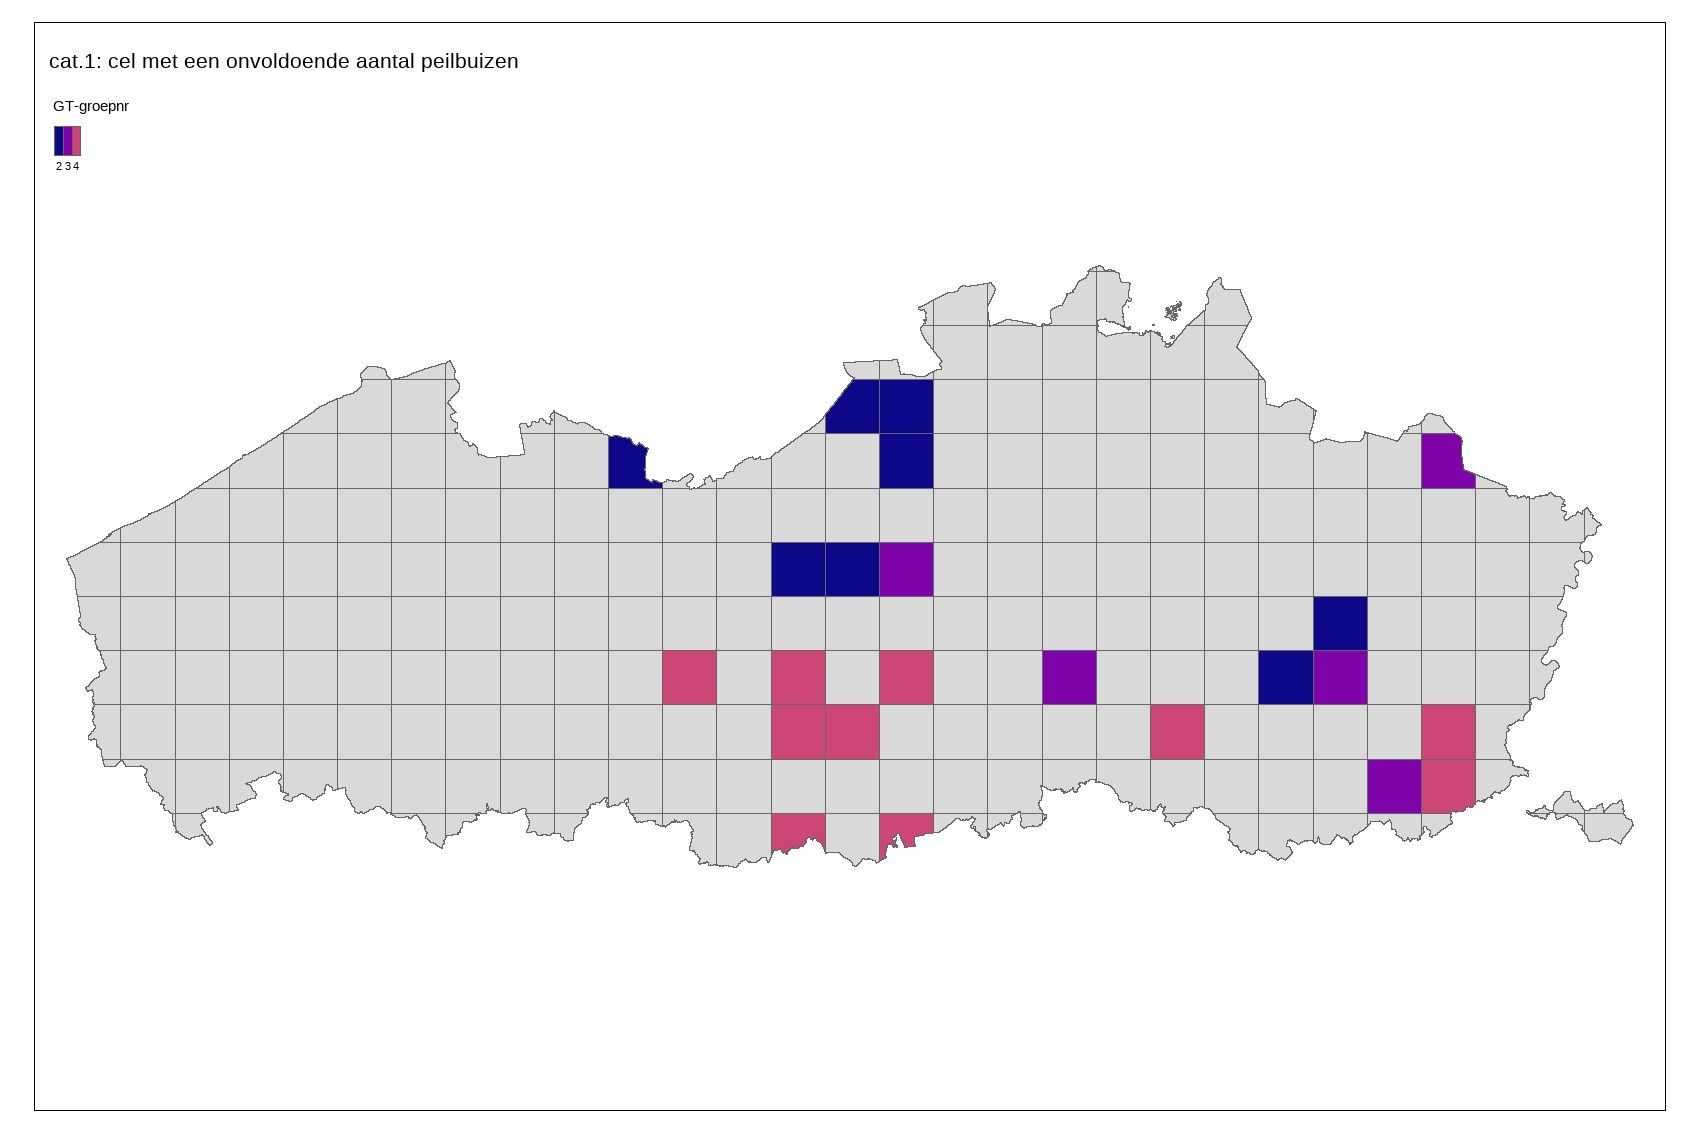
\includegraphics{droogtemeetnet_ontwerp_files/figure-latex/cat1A-plot-1.pdf}
Er zijn 21 gewenste meetlocaties zonder peilbuis, verspreid over 21
rastercellen (figuur \ref{fig:cat1A-plot}). De hiaten zijn bijgevolg
ruimtelijk goed verdeeld.

\subsection{Het instellen van
kwaliteitscriteria}\label{het-instellen-van-kwaliteitscriteria}

Er liggen 1003 peilbuizen in de geselecteerde rastercellen. Dit aantal
is te groot om op alle meetreeksen een tijdreeksanalyse toe te passen.
We willen dit aantal reduceren. De meetreeksen van peilbuizen in
rastercellen van categorie 1 en 2 zullen sowieso moeten geanalyseerd
worden. Voor rastercellen van categorie willen we het aantal analyses
beperken door eerst de meetreeksen met de (relatief) beste kwaliteit
(zie \href{basiskwaliteitscriteria}{hier}) te analyseren. We blijven
meetreeksen analyseren tot wanneer het aantal geschikte reeksen gelijk
of groter is dan het gewenste aantal.

De kwaliteitscriteria werden enkel gebruikt om de peilbuizen in klassen
te verdelen en binnen een rastercel en GT-groep de peilbuizen met
\textbf{relatief} de beste reeksen aan te duiden. Er werden geen
absolute minimale vereisten aan een tijdreeks opgelegd.

We vormen de clusters in een aantal stappen. Eerst klasseren en
rangschikken we de opnamen volgens de eerste twee criteria (aantal
meetjaren en het laatste meetjaar) afzonderlijk. Tabel
\ref{tab:berekenen-clusters-criteria} geeft een overzicht van deze
indeling. Ze geeft per rastercel en GTgroep voor alle voorkomende
combinaties van jaartal van de recentste meting en van de lengte van de
tijdreeks de rang van elk van beide.

\begin{table}

\caption{\label{tab:berekenen-clusters-criteria}Indeling van de peilbuizen in clusters o.b.v. twee criteria}
\centering
\begin{tabular}[t]{r|r|r|r|r|r|r|r}
\hline
rastercelnummer & GTgroep & \# gezochte meetptn & recentste lg3-jaar & aantal jaren met lg3 & \# peilbuizen & rang spreiding & rang lengte tijdreeks\\
\hline
1 & 5 & 1 & 2009 & 1 & 8 & 1 & 1\\
\hline
1 & 5 & 1 & 0 & 0 & 5 & 402 & 1\\
\hline
25 & 4 & 1 & 2003 & 1 & 1 & 1 & 1\\
\hline
41 & 2 & 1 & 2007 & 2 & 2 & 1 & 1\\
\hline
46 & 5 & 1 & 0 & 0 & 3 & 1 & 1\\
\hline
53 & 5 & 1 & 0 & 0 & 2 & 1 & 1\\
\hline
54 & 2 & 1 & 0 & 0 & 9 & 1 & 1\\
\hline
54 & 3 & 1 & 2016 & 4 & 3 & 1 & 1\\
\hline
54 & 3 & 1 & 2010 & 2 & 1 & 2 & 1\\
\hline
54 & 3 & 1 & 2006 & 1 & 7 & 3 & 1\\
\hline
54 & 3 & 1 & 0 & 0 & 10 & 404 & 1\\
\hline
57 & 4 & 1 & 2010 & 4 & 2 & 1 & 1\\
\hline
89 & 4 & 1 & 2003 & 1 & 1 & 1 & 1\\
\hline
89 & 4 & 1 & 0 & 0 & 4 & 401 & 1\\
\hline
113 & 5 & 1 & 2009 & 5 & 2 & 1 & 1\\
\hline
113 & 5 & 1 & 2004 & 3 & 2 & 2 & 1\\
\hline
113 & 5 & 1 & 2004 & 2 & 2 & 2 & 1\\
\hline
113 & 5 & 1 & 2009 & 1 & 1 & 1 & 1\\
\hline
113 & 5 & 1 & 0 & 0 & 2 & 402 & 2\\
\hline
118 & 1 & 1 & 2009 & 9 & 13 & 2 & 1\\
\hline
118 & 1 & 1 & 2009 & 7 & 1 & 2 & 1\\
\hline
118 & 1 & 1 & 2015 & 5 & 1 & 1 & 1\\
\hline
118 & 1 & 1 & 2009 & 4 & 2 & 2 & 2\\
\hline
118 & 1 & 1 & 0 & 0 & 21 & 404 & 2\\
\hline
134 & 1 & 1 & 2015 & 9 & 2 & 1 & 1\\
\hline
134 & 1 & 1 & 2012 & 6 & 1 & 1 & 1\\
\hline
134 & 1 & 1 & 2011 & 6 & 1 & 1 & 1\\
\hline
134 & 1 & 1 & 2010 & 4 & 1 & 2 & 2\\
\hline
134 & 1 & 1 & 2009 & 4 & 1 & 2 & 2\\
\hline
134 & 1 & 1 & 2011 & 3 & 1 & 1 & 2\\
\hline
134 & 1 & 1 & 0 & 0 & 70 & 404 & 2\\
\hline
134 & 4 & 1 & 2013 & 6 & 2 & 1 & 1\\
\hline
134 & 4 & 1 & 2016 & 4 & 1 & 1 & 1\\
\hline
134 & 4 & 1 & 0 & 0 & 5 & 404 & 2\\
\hline
134 & 5 & 1 & 0 & 0 & 1 & 1 & 1\\
\hline
146 & 1 & 1 & 2016 & 9 & 1 & 1 & 1\\
\hline
146 & 1 & 1 & 2016 & 5 & 1 & 1 & 1\\
\hline
146 & 1 & 1 & 2003 & 3 & 3 & 3 & 2\\
\hline
146 & 1 & 1 & 2001 & 1 & 4 & 4 & 2\\
\hline
146 & 1 & 1 & 0 & 0 & 4 & 404 & 2\\
\hline
166 & 2 & 1 & 2016 & 3 & 2 & 1 & 1\\
\hline
166 & 2 & 1 & 2013 & 2 & 1 & 1 & 1\\
\hline
166 & 2 & 1 & 0 & 0 & 15 & 404 & 1\\
\hline
177 & 4 & 1 & 2012 & 12 & 11 & 1 & 1\\
\hline
177 & 4 & 1 & 2012 & 11 & 3 & 1 & 1\\
\hline
177 & 4 & 1 & 2011 & 11 & 1 & 2 & 1\\
\hline
177 & 4 & 1 & 2012 & 10 & 1 & 1 & 1\\
\hline
177 & 4 & 1 & 2011 & 10 & 2 & 2 & 1\\
\hline
177 & 4 & 1 & 2012 & 9 & 1 & 1 & 1\\
\hline
177 & 4 & 1 & 2011 & 9 & 1 & 2 & 1\\
\hline
177 & 4 & 1 & 2015 & 7 & 1 & 1 & 2\\
\hline
177 & 4 & 1 & 2007 & 7 & 5 & 2 & 2\\
\hline
177 & 4 & 1 & 2007 & 6 & 1 & 2 & 2\\
\hline
177 & 4 & 1 & 2007 & 5 & 1 & 2 & 2\\
\hline
177 & 4 & 1 & 2006 & 5 & 2 & 3 & 2\\
\hline
177 & 4 & 1 & 2016 & 4 & 1 & 1 & 2\\
\hline
177 & 4 & 1 & 2012 & 4 & 1 & 1 & 2\\
\hline
177 & 4 & 1 & 2006 & 4 & 2 & 3 & 2\\
\hline
177 & 4 & 1 & 2012 & 3 & 2 & 1 & 2\\
\hline
177 & 4 & 1 & 2011 & 3 & 2 & 2 & 2\\
\hline
177 & 4 & 1 & 2006 & 3 & 1 & 3 & 2\\
\hline
177 & 4 & 1 & 2012 & 1 & 1 & 1 & 3\\
\hline
177 & 4 & 1 & 2006 & 1 & 3 & 3 & 3\\
\hline
177 & 4 & 1 & 2002 & 1 & 1 & 3 & 3\\
\hline
177 & 4 & 1 & 0 & 0 & 25 & 404 & 3\\
\hline
177 & 5 & 1 & 2006 & 5 & 8 & 1 & 1\\
\hline
177 & 5 & 1 & 2008 & 4 & 1 & 1 & 1\\
\hline
177 & 5 & 1 & 2006 & 2 & 1 & 1 & 1\\
\hline
177 & 5 & 1 & 2003 & 2 & 1 & 2 & 1\\
\hline
177 & 5 & 1 & 2006 & 1 & 1 & 1 & 1\\
\hline
177 & 5 & 1 & 0 & 0 & 3 & 402 & 2\\
\hline
185 & 4 & 1 & 2015 & 8 & 1 & 1 & 1\\
\hline
185 & 4 & 1 & 2012 & 5 & 1 & 1 & 1\\
\hline
185 & 4 & 1 & 0 & 0 & 1 & 404 & 2\\
\hline
198 & 4 & 1 & 2016 & 12 & 1 & 1 & 1\\
\hline
198 & 4 & 1 & 2014 & 6 & 1 & 1 & 2\\
\hline
198 & 4 & 1 & 2015 & 4 & 1 & 1 & 2\\
\hline
198 & 4 & 1 & 2010 & 4 & 1 & 2 & 2\\
\hline
198 & 4 & 1 & 2006 & 2 & 1 & 3 & 3\\
\hline
198 & 4 & 1 & 2005 & 1 & 1 & 3 & 3\\
\hline
198 & 4 & 1 & 0 & 0 & 5 & 404 & 3\\
\hline
210 & 3 & 1 & 2015 & 11 & 1 & 1 & 1\\
\hline
210 & 3 & 1 & 2016 & 10 & 1 & 1 & 1\\
\hline
210 & 3 & 1 & 2016 & 6 & 1 & 1 & 2\\
\hline
210 & 3 & 1 & 2014 & 4 & 1 & 1 & 2\\
\hline
210 & 3 & 1 & 0 & 0 & 2 & 404 & 3\\
\hline
217 & 3 & 1 & 2008 & 1 & 2 & 1 & 1\\
\hline
217 & 3 & 1 & 2003 & 1 & 1 & 2 & 1\\
\hline
217 & 3 & 1 & 0 & 0 & 5 & 402 & 1\\
\hline
217 & 4 & 1 & 2012 & 3 & 2 & 1 & 1\\
\hline
217 & 4 & 1 & 2009 & 2 & 1 & 1 & 1\\
\hline
217 & 4 & 1 & 2003 & 1 & 1 & 2 & 1\\
\hline
233 & 1 & 1 & 2015 & 8 & 1 & 1 & 1\\
\hline
233 & 2 & 1 & 2012 & 11 & 1 & 1 & 1\\
\hline
262 & 2 & 1 & 2016 & 5 & 1 & 1 & 1\\
\hline
262 & 2 & 1 & 2012 & 2 & 1 & 1 & 1\\
\hline
262 & 2 & 1 & 2001 & 1 & 1 & 4 & 1\\
\hline
262 & 2 & 1 & 0 & 0 & 6 & 404 & 2\\
\hline
262 & 3 & 1 & 2008 & 2 & 10 & 2 & 1\\
\hline
262 & 3 & 1 & 2016 & 1 & 1 & 1 & 1\\
\hline
262 & 3 & 1 & 2008 & 1 & 3 & 2 & 1\\
\hline
262 & 3 & 1 & 2004 & 1 & 1 & 3 & 1\\
\hline
262 & 3 & 1 & 2001 & 1 & 6 & 4 & 1\\
\hline
262 & 3 & 1 & 0 & 0 & 12 & 404 & 1\\
\hline
262 & 4 & 1 & 2016 & 10 & 1 & 1 & 1\\
\hline
262 & 4 & 1 & 2010 & 5 & 2 & 2 & 2\\
\hline
262 & 4 & 1 & 2008 & 2 & 6 & 2 & 2\\
\hline
262 & 4 & 1 & 2006 & 1 & 1 & 3 & 2\\
\hline
262 & 4 & 1 & 2001 & 1 & 1 & 4 & 2\\
\hline
262 & 4 & 1 & 0 & 0 & 27 & 404 & 3\\
\hline
274 & 2 & 1 & 2015 & 14 & 1 & 1 & 1\\
\hline
274 & 2 & 1 & 0 & 0 & 1 & 404 & 3\\
\hline
306 & 1 & 1 & 2016 & 5 & 4 & 1 & 1\\
\hline
306 & 2 & 1 & 0 & 0 & 1 & 1 & 1\\
\hline
309 & 5 & 1 & 2015 & 11 & 2 & 1 & 1\\
\hline
309 & 5 & 1 & 2015 & 10 & 2 & 1 & 1\\
\hline
309 & 5 & 1 & 2013 & 10 & 1 & 1 & 1\\
\hline
309 & 5 & 1 & 2012 & 9 & 1 & 1 & 1\\
\hline
309 & 5 & 1 & 2014 & 6 & 1 & 1 & 2\\
\hline
309 & 5 & 1 & 2009 & 5 & 1 & 2 & 2\\
\hline
309 & 5 & 1 & 2010 & 1 & 1 & 2 & 3\\
\hline
309 & 5 & 1 & 0 & 0 & 1 & 404 & 3\\
\hline
310 & 2 & 1 & 2003 & 3 & 1 & 1 & 1\\
\hline
310 & 2 & 1 & 2003 & 2 & 1 & 1 & 1\\
\hline
310 & 2 & 1 & 2002 & 2 & 2 & 1 & 1\\
\hline
310 & 2 & 1 & 2003 & 1 & 1 & 1 & 1\\
\hline
310 & 2 & 1 & 2001 & 1 & 1 & 1 & 1\\
\hline
310 & 2 & 1 & 0 & 0 & 2 & 401 & 1\\
\hline
310 & 3 & 1 & 2016 & 10 & 1 & 1 & 1\\
\hline
310 & 3 & 1 & 2002 & 2 & 5 & 3 & 2\\
\hline
310 & 3 & 1 & 2002 & 1 & 3 & 3 & 2\\
\hline
310 & 3 & 1 & 2001 & 1 & 14 & 4 & 2\\
\hline
310 & 3 & 1 & 0 & 0 & 29 & 404 & 3\\
\hline
342 & 1 & 1 & 2016 & 9 & 1 & 1 & 1\\
\hline
342 & 1 & 1 & 2012 & 8 & 1 & 1 & 1\\
\hline
342 & 1 & 1 & 2016 & 6 & 1 & 1 & 1\\
\hline
342 & 1 & 1 & 2012 & 6 & 1 & 1 & 1\\
\hline
342 & 1 & 1 & 2011 & 5 & 1 & 2 & 1\\
\hline
390 & 4 & 1 & 0 & 0 & 8 & 1 & 1\\
\hline
437 & 5 & 1 & 0 & 0 & 4 & 1 & 1\\
\hline
438 & 2 & 1 & 2016 & 5 & 1 & 1 & 1\\
\hline
438 & 2 & 1 & 2016 & 4 & 2 & 1 & 1\\
\hline
438 & 2 & 1 & 2014 & 2 & 1 & 1 & 1\\
\hline
438 & 2 & 1 & 2006 & 1 & 3 & 3 & 1\\
\hline
438 & 2 & 1 & 0 & 0 & 1 & 404 & 2\\
\hline
438 & 3 & 1 & 2015 & 3 & 1 & 1 & 1\\
\hline
438 & 3 & 1 & 2006 & 1 & 4 & 2 & 1\\
\hline
438 & 3 & 1 & 0 & 0 & 12 & 404 & 1\\
\hline
454 & 4 & 1 & 2013 & 9 & 5 & 1 & 1\\
\hline
470 & 1 & 1 & 2004 & 3 & 1 & 1 & 1\\
\hline
470 & 1 & 1 & 0 & 0 & 16 & 401 & 1\\
\hline
478 & 3 & 1 & 2010 & 3 & 1 & 1 & 1\\
\hline
478 & 3 & 1 & 2001 & 1 & 11 & 2 & 1\\
\hline
478 & 3 & 1 & 0 & 0 & 10 & 403 & 1\\
\hline
486 & 2 & 1 & 2005 & 1 & 1 & 1 & 1\\
\hline
486 & 2 & 1 & 0 & 0 & 3 & 402 & 1\\
\hline
537 & 4 & 1 & 2010 & 1 & 1 & 1 & 1\\
\hline
565 & 1 & 1 & 0 & 0 & 7 & 1 & 1\\
\hline
582 & 4 & 1 & 2016 & 10 & 1 & 1 & 1\\
\hline
582 & 4 & 1 & 2004 & 2 & 1 & 3 & 2\\
\hline
582 & 4 & 1 & 0 & 0 & 4 & 404 & 3\\
\hline
601 & 4 & 1 & 2008 & 5 & 2 & 1 & 1\\
\hline
601 & 4 & 1 & 2006 & 3 & 1 & 1 & 1\\
\hline
630 & 1 & 1 & 2014 & 9 & 3 & 1 & 1\\
\hline
630 & 1 & 1 & 2016 & 2 & 2 & 1 & 2\\
\hline
630 & 1 & 1 & 2016 & 1 & 1 & 1 & 2\\
\hline
630 & 1 & 1 & 2015 & 1 & 1 & 1 & 2\\
\hline
630 & 3 & 1 & 2016 & 4 & 2 & 1 & 1\\
\hline
630 & 3 & 1 & 2016 & 2 & 2 & 1 & 1\\
\hline
630 & 3 & 1 & 2015 & 1 & 1 & 1 & 1\\
\hline
630 & 3 & 1 & 0 & 0 & 3 & 404 & 1\\
\hline
693 & 2 & 1 & 0 & 0 & 2 & 1 & 1\\
\hline
693 & 3 & 1 & 2014 & 1 & 2 & 1 & 1\\
\hline
693 & 3 & 1 & 2011 & 1 & 6 & 1 & 1\\
\hline
693 & 3 & 1 & 0 & 0 & 10 & 403 & 1\\
\hline
693 & 5 & 1 & 0 & 0 & 8 & 1 & 1\\
\hline
694 & 1 & 1 & 0 & 0 & 4 & 1 & 1\\
\hline
694 & 3 & 1 & 2014 & 2 & 2 & 1 & 1\\
\hline
694 & 3 & 1 & 0 & 0 & 2 & 403 & 1\\
\hline
710 & 4 & 1 & 2010 & 6 & 1 & 1 & 1\\
\hline
710 & 4 & 1 & 2014 & 3 & 1 & 1 & 1\\
\hline
722 & 1 & 1 & 2016 & 10 & 1 & 1 & 1\\
\hline
722 & 1 & 1 & 2016 & 9 & 2 & 1 & 1\\
\hline
722 & 1 & 1 & 2016 & 7 & 1 & 1 & 1\\
\hline
722 & 1 & 1 & 2016 & 6 & 2 & 1 & 1\\
\hline
722 & 1 & 1 & 2016 & 5 & 1 & 1 & 2\\
\hline
722 & 1 & 1 & 2008 & 1 & 1 & 2 & 2\\
\hline
722 & 1 & 1 & 0 & 0 & 15 & 404 & 3\\
\hline
722 & 3 & 1 & 2016 & 9 & 1 & 1 & 1\\
\hline
722 & 3 & 1 & 2016 & 7 & 1 & 1 & 1\\
\hline
722 & 3 & 1 & 2014 & 7 & 1 & 1 & 1\\
\hline
722 & 3 & 1 & 2016 & 5 & 1 & 1 & 1\\
\hline
722 & 3 & 1 & 2014 & 5 & 1 & 1 & 1\\
\hline
722 & 3 & 1 & 2016 & 1 & 1 & 1 & 2\\
\hline
722 & 3 & 1 & 2008 & 1 & 2 & 2 & 2\\
\hline
722 & 3 & 1 & 0 & 0 & 7 & 404 & 2\\
\hline
734 & 3 & 1 & 2015 & 5 & 2 & 1 & 1\\
\hline
734 & 3 & 1 & 2016 & 3 & 2 & 1 & 1\\
\hline
734 & 3 & 1 & 0 & 0 & 17 & 404 & 2\\
\hline
734 & 5 & 1 & 0 & 0 & 4 & 1 & 1\\
\hline
745 & 3 & 2 & 2002 & 2 & 2 & 1 & 1\\
\hline
745 & 3 & 2 & 0 & 0 & 20 & 401 & 1\\
\hline
758 & 1 & 1 & 0 & 0 & 1 & 1 & 1\\
\hline
817 & 4 & 1 & 2012 & 10 & 3 & 1 & 1\\
\hline
817 & 4 & 1 & 2010 & 9 & 2 & 1 & 1\\
\hline
817 & 4 & 1 & 2012 & 8 & 1 & 1 & 1\\
\hline
817 & 4 & 1 & 2012 & 7 & 4 & 1 & 1\\
\hline
817 & 4 & 1 & 2013 & 6 & 2 & 1 & 1\\
\hline
817 & 4 & 1 & 2012 & 6 & 2 & 1 & 1\\
\hline
817 & 4 & 1 & 2008 & 6 & 1 & 2 & 1\\
\hline
817 & 4 & 1 & 2007 & 6 & 2 & 2 & 1\\
\hline
817 & 4 & 1 & 2013 & 5 & 1 & 1 & 2\\
\hline
817 & 4 & 1 & 2008 & 5 & 1 & 2 & 2\\
\hline
817 & 4 & 1 & 2006 & 2 & 1 & 2 & 2\\
\hline
817 & 4 & 1 & 0 & 0 & 15 & 403 & 3\\
\hline
817 & 5 & 1 & 2012 & 12 & 1 & 1 & 1\\
\hline
817 & 5 & 1 & 2012 & 10 & 1 & 1 & 1\\
\hline
817 & 5 & 1 & 2012 & 8 & 1 & 1 & 1\\
\hline
817 & 5 & 1 & 2007 & 6 & 3 & 2 & 2\\
\hline
817 & 5 & 1 & 2009 & 4 & 1 & 1 & 2\\
\hline
817 & 5 & 1 & 2004 & 4 & 1 & 2 & 2\\
\hline
817 & 5 & 1 & 2004 & 3 & 1 & 2 & 2\\
\hline
817 & 5 & 1 & 2006 & 2 & 1 & 2 & 3\\
\hline
817 & 5 & 1 & 0 & 0 & 7 & 403 & 3\\
\hline
822 & 1 & 1 & 2011 & 3 & 6 & 1 & 1\\
\hline
822 & 1 & 1 & 2009 & 2 & 1 & 1 & 1\\
\hline
822 & 1 & 1 & 2009 & 1 & 1 & 1 & 1\\
\hline
822 & 1 & 1 & 2005 & 1 & 1 & 2 & 1\\
\hline
822 & 1 & 1 & 2003 & 1 & 3 & 2 & 1\\
\hline
822 & 1 & 1 & 0 & 0 & 5 & 403 & 1\\
\hline
822 & 3 & 1 & 2009 & 4 & 1 & 1 & 1\\
\hline
822 & 3 & 1 & 2011 & 3 & 2 & 1 & 1\\
\hline
822 & 3 & 1 & 2009 & 3 & 1 & 1 & 1\\
\hline
822 & 3 & 1 & 2003 & 2 & 1 & 2 & 1\\
\hline
822 & 3 & 1 & 2009 & 1 & 4 & 1 & 1\\
\hline
822 & 3 & 1 & 2005 & 1 & 2 & 2 & 1\\
\hline
822 & 3 & 1 & 0 & 0 & 3 & 403 & 1\\
\hline
850 & 1 & 1 & 2014 & 3 & 1 & 1 & 1\\
\hline
850 & 1 & 1 & 0 & 0 & 4 & 403 & 1\\
\hline
886 & 1 & 1 & 2014 & 8 & 1 & 1 & 1\\
\hline
886 & 1 & 1 & 2011 & 6 & 1 & 2 & 1\\
\hline
886 & 1 & 1 & 2016 & 5 & 1 & 1 & 1\\
\hline
886 & 1 & 1 & 2012 & 5 & 1 & 1 & 1\\
\hline
886 & 1 & 1 & 2015 & 4 & 1 & 1 & 1\\
\hline
886 & 1 & 1 & 2011 & 4 & 2 & 2 & 1\\
\hline
886 & 1 & 1 & 2012 & 3 & 1 & 1 & 2\\
\hline
886 & 1 & 1 & 2011 & 1 & 1 & 2 & 2\\
\hline
886 & 1 & 1 & 0 & 0 & 3 & 404 & 2\\
\hline
886 & 2 & 1 & 2014 & 7 & 2 & 1 & 1\\
\hline
886 & 2 & 1 & 2011 & 6 & 1 & 1 & 1\\
\hline
886 & 2 & 1 & 2014 & 4 & 1 & 1 & 1\\
\hline
886 & 2 & 1 & 0 & 0 & 2 & 403 & 2\\
\hline
886 & 3 & 1 & 2014 & 7 & 8 & 1 & 1\\
\hline
886 & 3 & 1 & 2012 & 7 & 1 & 1 & 1\\
\hline
886 & 3 & 1 & 2014 & 6 & 1 & 1 & 1\\
\hline
886 & 3 & 1 & 2016 & 5 & 3 & 1 & 1\\
\hline
886 & 3 & 1 & 2011 & 2 & 1 & 2 & 2\\
\hline
886 & 3 & 1 & 0 & 0 & 12 & 404 & 2\\
\hline
918 & 1 & 1 & 2009 & 1 & 1 & 1 & 1\\
\hline
918 & 1 & 1 & 0 & 0 & 3 & 402 & 1\\
\hline
918 & 5 & 1 & 0 & 0 & 1 & 1 & 1\\
\hline
950 & 1 & 2 & 2016 & 13 & 1 & 1 & 1\\
\hline
950 & 1 & 2 & 2016 & 12 & 1 & 1 & 1\\
\hline
950 & 1 & 2 & 2015 & 11 & 1 & 1 & 1\\
\hline
950 & 1 & 2 & 2016 & 10 & 3 & 1 & 1\\
\hline
950 & 1 & 2 & 2016 & 8 & 2 & 1 & 2\\
\hline
950 & 1 & 2 & 2016 & 7 & 2 & 1 & 2\\
\hline
950 & 1 & 2 & 2016 & 6 & 3 & 1 & 2\\
\hline
950 & 1 & 2 & 2016 & 5 & 1 & 1 & 2\\
\hline
950 & 1 & 2 & 2016 & 4 & 1 & 1 & 2\\
\hline
950 & 1 & 2 & 2008 & 3 & 4 & 2 & 3\\
\hline
950 & 1 & 2 & 2005 & 2 & 3 & 3 & 3\\
\hline
950 & 1 & 2 & 0 & 0 & 45 & 404 & 3\\
\hline
950 & 3 & 1 & 2016 & 9 & 1 & 1 & 1\\
\hline
950 & 3 & 1 & 2016 & 6 & 1 & 1 & 1\\
\hline
950 & 3 & 1 & 2014 & 4 & 1 & 1 & 2\\
\hline
950 & 3 & 1 & 2008 & 2 & 1 & 2 & 2\\
\hline
950 & 3 & 1 & 0 & 0 & 15 & 404 & 2\\
\hline
950 & 5 & 1 & 2016 & 8 & 1 & 1 & 1\\
\hline
950 & 5 & 1 & 0 & 0 & 5 & 404 & 2\\
\hline
985 & 4 & 1 & 2012 & 4 & 1 & 1 & 1\\
\hline
985 & 4 & 1 & 2010 & 2 & 1 & 1 & 1\\
\hline
985 & 4 & 1 & 0 & 0 & 5 & 403 & 1\\
\hline
1010 & 1 & 1 & 2016 & 10 & 2 & 1 & 1\\
\hline
1010 & 1 & 1 & 2016 & 9 & 1 & 1 & 1\\
\hline
1010 & 1 & 1 & 2016 & 5 & 1 & 1 & 2\\
\hline
1010 & 1 & 1 & 2009 & 4 & 4 & 2 & 2\\
\hline
1010 & 1 & 1 & 0 & 0 & 9 & 404 & 3\\
\hline
1014 & 1 & 1 & 2006 & 1 & 1 & 1 & 1\\
\hline
1014 & 1 & 1 & 0 & 0 & 2 & 402 & 1\\
\hline
1017 & 3 & 1 & 0 & 0 & 3 & 1 & 1\\
\hline
\end{tabular}
\end{table}

We groeperen vervolgens de peilbuizen (naast rastercel en GTgroep) voor
elke voorkomende combinatie van de twee criteria (zie tabel
\ref{tab:synthese-clusters-extra-criteria}). We berekenen voor deze
combinaties een rangorde, waarbij ook het
\protect\hyperlink{suppl-criteria}{vierde kwaliteitscriterium} in
rekening gebracht wordt (= rang combi in de tabel). Peilbuizen in
clusters met een lagere rang combi-waarde zullen voorrang krijgen.

We berekenen ook het hoogste rangnummer dat nodig is om in het resterend
gewenste aantal peilbuizen te kunnen voorzien (= max rang).

\begin{table}

\caption{\label{tab:synthese-clusters-extra-criteria}Overzicht clustering o.b.v. de drie kwaliteitscriteria}
\centering
\begin{tabular}[t]{r|r|r|r|r|r|r|r}
\hline
rastercelnummer & GTgroep & gewenst \# meetptn & \# peilbuizen & rang spreiding & rang lengte tijdreeks & rang combi & max rang\\
\hline
1 & 5 & 1 & 8 & 1 & 1 & 1 & 1\\
\hline
1 & 5 & 1 & 5 & 402 & 1 & 2 & 1\\
\hline
25 & 4 & 1 & 1 & 1 & 1 & 1 & 1\\
\hline
41 & 2 & 1 & 2 & 1 & 1 & 1 & 1\\
\hline
46 & 5 & 1 & 3 & 1 & 1 & 1 & 1\\
\hline
53 & 5 & 1 & 2 & 1 & 1 & 1 & 1\\
\hline
54 & 2 & 1 & 9 & 1 & 1 & 1 & 1\\
\hline
54 & 3 & 1 & 3 & 1 & 1 & 1 & 1\\
\hline
54 & 3 & 1 & 1 & 2 & 1 & 2 & 1\\
\hline
54 & 3 & 1 & 7 & 3 & 1 & 3 & 1\\
\hline
54 & 3 & 1 & 10 & 404 & 1 & 4 & 1\\
\hline
57 & 4 & 1 & 2 & 1 & 1 & 1 & 1\\
\hline
89 & 4 & 1 & 1 & 1 & 1 & 1 & 1\\
\hline
89 & 4 & 1 & 4 & 401 & 1 & 2 & 1\\
\hline
113 & 5 & 1 & 3 & 1 & 1 & 1 & 1\\
\hline
113 & 5 & 1 & 4 & 2 & 1 & 2 & 1\\
\hline
113 & 5 & 1 & 2 & 402 & 2 & 3 & 1\\
\hline
118 & 1 & 1 & 1 & 1 & 1 & 1 & 1\\
\hline
118 & 1 & 1 & 14 & 2 & 1 & 2 & 1\\
\hline
118 & 1 & 1 & 2 & 2 & 2 & 3 & 1\\
\hline
118 & 1 & 1 & 21 & 404 & 2 & 4 & 1\\
\hline
134 & 1 & 1 & 4 & 1 & 1 & 1 & 1\\
\hline
134 & 1 & 1 & 1 & 1 & 2 & 2 & 1\\
\hline
134 & 1 & 1 & 2 & 2 & 2 & 3 & 1\\
\hline
134 & 1 & 1 & 70 & 404 & 2 & 4 & 1\\
\hline
134 & 4 & 1 & 3 & 1 & 1 & 1 & 1\\
\hline
134 & 4 & 1 & 5 & 404 & 2 & 2 & 1\\
\hline
134 & 5 & 1 & 1 & 1 & 1 & 1 & 1\\
\hline
146 & 1 & 1 & 2 & 1 & 1 & 1 & 1\\
\hline
146 & 1 & 1 & 3 & 3 & 2 & 2 & 1\\
\hline
146 & 1 & 1 & 4 & 4 & 2 & 3 & 1\\
\hline
146 & 1 & 1 & 4 & 404 & 2 & 4 & 1\\
\hline
166 & 2 & 1 & 3 & 1 & 1 & 1 & 1\\
\hline
166 & 2 & 1 & 15 & 404 & 1 & 2 & 1\\
\hline
177 & 4 & 1 & 16 & 1 & 1 & 1 & 1\\
\hline
177 & 4 & 1 & 5 & 1 & 2 & 2 & 1\\
\hline
177 & 4 & 1 & 1 & 1 & 3 & 3 & 1\\
\hline
177 & 4 & 1 & 4 & 2 & 1 & 4 & 1\\
\hline
177 & 4 & 1 & 9 & 2 & 2 & 5 & 1\\
\hline
177 & 4 & 1 & 5 & 3 & 2 & 6 & 1\\
\hline
177 & 4 & 1 & 4 & 3 & 3 & 7 & 1\\
\hline
177 & 4 & 1 & 25 & 404 & 3 & 8 & 1\\
\hline
177 & 5 & 1 & 11 & 1 & 1 & 1 & 1\\
\hline
177 & 5 & 1 & 1 & 2 & 1 & 2 & 1\\
\hline
177 & 5 & 1 & 3 & 402 & 2 & 3 & 1\\
\hline
185 & 4 & 1 & 2 & 1 & 1 & 1 & 1\\
\hline
185 & 4 & 1 & 1 & 404 & 2 & 2 & 1\\
\hline
198 & 4 & 1 & 1 & 1 & 1 & 1 & 1\\
\hline
198 & 4 & 1 & 2 & 1 & 2 & 2 & 1\\
\hline
198 & 4 & 1 & 1 & 2 & 2 & 3 & 1\\
\hline
198 & 4 & 1 & 2 & 3 & 3 & 4 & 1\\
\hline
198 & 4 & 1 & 5 & 404 & 3 & 5 & 1\\
\hline
210 & 3 & 1 & 2 & 1 & 1 & 1 & 1\\
\hline
210 & 3 & 1 & 2 & 1 & 2 & 2 & 1\\
\hline
210 & 3 & 1 & 2 & 404 & 3 & 3 & 1\\
\hline
217 & 3 & 1 & 2 & 1 & 1 & 1 & 1\\
\hline
217 & 3 & 1 & 1 & 2 & 1 & 2 & 1\\
\hline
217 & 3 & 1 & 5 & 402 & 1 & 3 & 1\\
\hline
217 & 4 & 1 & 3 & 1 & 1 & 1 & 1\\
\hline
217 & 4 & 1 & 1 & 2 & 1 & 2 & 1\\
\hline
233 & 1 & 1 & 1 & 1 & 1 & 1 & 1\\
\hline
233 & 2 & 1 & 1 & 1 & 1 & 1 & 1\\
\hline
262 & 2 & 1 & 2 & 1 & 1 & 1 & 1\\
\hline
262 & 2 & 1 & 1 & 4 & 1 & 2 & 1\\
\hline
262 & 2 & 1 & 6 & 404 & 2 & 3 & 1\\
\hline
262 & 3 & 1 & 1 & 1 & 1 & 1 & 1\\
\hline
262 & 3 & 1 & 13 & 2 & 1 & 2 & 1\\
\hline
262 & 3 & 1 & 1 & 3 & 1 & 3 & 1\\
\hline
262 & 3 & 1 & 6 & 4 & 1 & 4 & 1\\
\hline
262 & 3 & 1 & 12 & 404 & 1 & 5 & 1\\
\hline
262 & 4 & 1 & 1 & 1 & 1 & 1 & 1\\
\hline
262 & 4 & 1 & 8 & 2 & 2 & 2 & 1\\
\hline
262 & 4 & 1 & 1 & 3 & 2 & 3 & 1\\
\hline
262 & 4 & 1 & 1 & 4 & 2 & 4 & 1\\
\hline
262 & 4 & 1 & 27 & 404 & 3 & 5 & 1\\
\hline
274 & 2 & 1 & 1 & 1 & 1 & 1 & 1\\
\hline
274 & 2 & 1 & 1 & 404 & 3 & 2 & 1\\
\hline
306 & 1 & 1 & 4 & 1 & 1 & 1 & 1\\
\hline
306 & 2 & 1 & 1 & 1 & 1 & 1 & 1\\
\hline
309 & 5 & 1 & 6 & 1 & 1 & 1 & 1\\
\hline
309 & 5 & 1 & 1 & 1 & 2 & 2 & 1\\
\hline
309 & 5 & 1 & 1 & 2 & 2 & 3 & 1\\
\hline
309 & 5 & 1 & 1 & 2 & 3 & 4 & 1\\
\hline
309 & 5 & 1 & 1 & 404 & 3 & 5 & 1\\
\hline
310 & 2 & 1 & 6 & 1 & 1 & 1 & 1\\
\hline
310 & 2 & 1 & 2 & 401 & 1 & 2 & 1\\
\hline
310 & 3 & 1 & 1 & 1 & 1 & 1 & 1\\
\hline
310 & 3 & 1 & 8 & 3 & 2 & 2 & 1\\
\hline
310 & 3 & 1 & 14 & 4 & 2 & 3 & 1\\
\hline
310 & 3 & 1 & 29 & 404 & 3 & 4 & 1\\
\hline
342 & 1 & 1 & 4 & 1 & 1 & 1 & 1\\
\hline
342 & 1 & 1 & 1 & 2 & 1 & 2 & 1\\
\hline
390 & 4 & 1 & 8 & 1 & 1 & 1 & 1\\
\hline
437 & 5 & 1 & 4 & 1 & 1 & 1 & 1\\
\hline
438 & 2 & 1 & 4 & 1 & 1 & 1 & 1\\
\hline
438 & 2 & 1 & 3 & 3 & 1 & 2 & 1\\
\hline
438 & 2 & 1 & 1 & 404 & 2 & 3 & 1\\
\hline
438 & 3 & 1 & 1 & 1 & 1 & 1 & 1\\
\hline
438 & 3 & 1 & 4 & 2 & 1 & 2 & 1\\
\hline
438 & 3 & 1 & 12 & 404 & 1 & 3 & 1\\
\hline
454 & 4 & 1 & 5 & 1 & 1 & 1 & 1\\
\hline
470 & 1 & 1 & 1 & 1 & 1 & 1 & 1\\
\hline
470 & 1 & 1 & 16 & 401 & 1 & 2 & 1\\
\hline
478 & 3 & 1 & 1 & 1 & 1 & 1 & 1\\
\hline
478 & 3 & 1 & 11 & 2 & 1 & 2 & 1\\
\hline
478 & 3 & 1 & 10 & 403 & 1 & 3 & 1\\
\hline
486 & 2 & 1 & 1 & 1 & 1 & 1 & 1\\
\hline
486 & 2 & 1 & 3 & 402 & 1 & 2 & 1\\
\hline
537 & 4 & 1 & 1 & 1 & 1 & 1 & 1\\
\hline
565 & 1 & 1 & 7 & 1 & 1 & 1 & 1\\
\hline
582 & 4 & 1 & 1 & 1 & 1 & 1 & 1\\
\hline
582 & 4 & 1 & 1 & 3 & 2 & 2 & 1\\
\hline
582 & 4 & 1 & 4 & 404 & 3 & 3 & 1\\
\hline
601 & 4 & 1 & 3 & 1 & 1 & 1 & 1\\
\hline
630 & 1 & 1 & 3 & 1 & 1 & 1 & 1\\
\hline
630 & 1 & 1 & 4 & 1 & 2 & 2 & 1\\
\hline
630 & 3 & 1 & 5 & 1 & 1 & 1 & 1\\
\hline
630 & 3 & 1 & 3 & 404 & 1 & 2 & 1\\
\hline
693 & 2 & 1 & 2 & 1 & 1 & 1 & 1\\
\hline
693 & 3 & 1 & 8 & 1 & 1 & 1 & 1\\
\hline
693 & 3 & 1 & 10 & 403 & 1 & 2 & 1\\
\hline
693 & 5 & 1 & 8 & 1 & 1 & 1 & 1\\
\hline
694 & 1 & 1 & 4 & 1 & 1 & 1 & 1\\
\hline
694 & 3 & 1 & 2 & 1 & 1 & 1 & 1\\
\hline
694 & 3 & 1 & 2 & 403 & 1 & 2 & 1\\
\hline
710 & 4 & 1 & 2 & 1 & 1 & 1 & 1\\
\hline
722 & 1 & 1 & 6 & 1 & 1 & 1 & 1\\
\hline
722 & 1 & 1 & 1 & 1 & 2 & 2 & 1\\
\hline
722 & 1 & 1 & 1 & 2 & 2 & 3 & 1\\
\hline
722 & 1 & 1 & 15 & 404 & 3 & 4 & 1\\
\hline
722 & 3 & 1 & 5 & 1 & 1 & 1 & 1\\
\hline
722 & 3 & 1 & 1 & 1 & 2 & 2 & 1\\
\hline
722 & 3 & 1 & 2 & 2 & 2 & 3 & 1\\
\hline
722 & 3 & 1 & 7 & 404 & 2 & 4 & 1\\
\hline
734 & 3 & 1 & 4 & 1 & 1 & 1 & 1\\
\hline
734 & 3 & 1 & 17 & 404 & 2 & 2 & 1\\
\hline
734 & 5 & 1 & 4 & 1 & 1 & 1 & 1\\
\hline
745 & 3 & 2 & 2 & 1 & 1 & 1 & 1\\
\hline
745 & 3 & 2 & 20 & 401 & 1 & 2 & 1\\
\hline
758 & 1 & 1 & 1 & 1 & 1 & 1 & 1\\
\hline
817 & 4 & 1 & 14 & 1 & 1 & 1 & 1\\
\hline
817 & 4 & 1 & 1 & 1 & 2 & 2 & 1\\
\hline
817 & 4 & 1 & 3 & 2 & 1 & 3 & 1\\
\hline
817 & 4 & 1 & 2 & 2 & 2 & 4 & 1\\
\hline
817 & 4 & 1 & 15 & 403 & 3 & 5 & 1\\
\hline
817 & 5 & 1 & 3 & 1 & 1 & 1 & 1\\
\hline
817 & 5 & 1 & 1 & 1 & 2 & 2 & 1\\
\hline
817 & 5 & 1 & 5 & 2 & 2 & 3 & 1\\
\hline
817 & 5 & 1 & 1 & 2 & 3 & 4 & 1\\
\hline
817 & 5 & 1 & 7 & 403 & 3 & 5 & 1\\
\hline
822 & 1 & 1 & 8 & 1 & 1 & 1 & 1\\
\hline
822 & 1 & 1 & 4 & 2 & 1 & 2 & 1\\
\hline
822 & 1 & 1 & 5 & 403 & 1 & 3 & 1\\
\hline
822 & 3 & 1 & 8 & 1 & 1 & 1 & 1\\
\hline
822 & 3 & 1 & 3 & 2 & 1 & 2 & 1\\
\hline
822 & 3 & 1 & 3 & 403 & 1 & 3 & 1\\
\hline
850 & 1 & 1 & 1 & 1 & 1 & 1 & 1\\
\hline
850 & 1 & 1 & 4 & 403 & 1 & 2 & 1\\
\hline
886 & 1 & 1 & 4 & 1 & 1 & 1 & 1\\
\hline
886 & 1 & 1 & 1 & 1 & 2 & 2 & 1\\
\hline
886 & 1 & 1 & 3 & 2 & 1 & 3 & 1\\
\hline
886 & 1 & 1 & 1 & 2 & 2 & 4 & 1\\
\hline
886 & 1 & 1 & 3 & 404 & 2 & 5 & 1\\
\hline
886 & 2 & 1 & 4 & 1 & 1 & 1 & 1\\
\hline
886 & 2 & 1 & 2 & 403 & 2 & 2 & 1\\
\hline
886 & 3 & 1 & 13 & 1 & 1 & 1 & 1\\
\hline
886 & 3 & 1 & 1 & 2 & 2 & 2 & 1\\
\hline
886 & 3 & 1 & 12 & 404 & 2 & 3 & 1\\
\hline
918 & 1 & 1 & 1 & 1 & 1 & 1 & 1\\
\hline
918 & 1 & 1 & 3 & 402 & 1 & 2 & 1\\
\hline
918 & 5 & 1 & 1 & 1 & 1 & 1 & 1\\
\hline
950 & 1 & 2 & 6 & 1 & 1 & 1 & 1\\
\hline
950 & 1 & 2 & 9 & 1 & 2 & 2 & 1\\
\hline
950 & 1 & 2 & 4 & 2 & 3 & 3 & 1\\
\hline
950 & 1 & 2 & 3 & 3 & 3 & 4 & 1\\
\hline
950 & 1 & 2 & 45 & 404 & 3 & 5 & 1\\
\hline
950 & 3 & 1 & 2 & 1 & 1 & 1 & 1\\
\hline
950 & 3 & 1 & 1 & 1 & 2 & 2 & 1\\
\hline
950 & 3 & 1 & 1 & 2 & 2 & 3 & 1\\
\hline
950 & 3 & 1 & 15 & 404 & 2 & 4 & 1\\
\hline
950 & 5 & 1 & 1 & 1 & 1 & 1 & 1\\
\hline
950 & 5 & 1 & 5 & 404 & 2 & 2 & 1\\
\hline
985 & 4 & 1 & 2 & 1 & 1 & 1 & 1\\
\hline
985 & 4 & 1 & 5 & 403 & 1 & 2 & 1\\
\hline
1010 & 1 & 1 & 3 & 1 & 1 & 1 & 1\\
\hline
1010 & 1 & 1 & 1 & 1 & 2 & 2 & 1\\
\hline
1010 & 1 & 1 & 4 & 2 & 2 & 3 & 1\\
\hline
1010 & 1 & 1 & 9 & 404 & 3 & 4 & 1\\
\hline
1014 & 1 & 1 & 1 & 1 & 1 & 1 & 1\\
\hline
1014 & 1 & 1 & 2 & 402 & 1 & 2 & 1\\
\hline
1017 & 3 & 1 & 3 & 1 & 1 & 1 & 1\\
\hline
\end{tabular}
\end{table}

\subsection{Categorie 2: Rastercellen met juist voldoende
peilbuizen}\label{cat2}

Wanneer voor een rastercel en een GTgroep het gewenste aantal meetpunten
gelijk is aan een som van het aantal beschikbare peilbuizen in een
cluster dan rekenen we die rastercel tot categorie 2. Tabel
\ref{tab:cat2-table} geeft hiervan het overzicht.

\begin{table}

\caption{\label{tab:cat2-table}Categorie 2: rastercellen met een juist voldoende aantal peilbuizen}
\centering
\begin{tabular}[t]{r|r|r|r|r|r|r}
\hline
rastercelnummer & GTgroep & gewenst \# meetptn & \# peilbuizen & rang cluster spreiding & rang cluster lengte tijdreeks & rang combi\\
\hline
25 & 4 & 1 & 1 & 1 & 1 & 1\\
\hline
134 & 5 & 1 & 1 & 1 & 1 & 1\\
\hline
233 & 1 & 1 & 1 & 1 & 1 & 1\\
\hline
233 & 2 & 1 & 1 & 1 & 1 & 1\\
\hline
306 & 2 & 1 & 1 & 1 & 1 & 1\\
\hline
537 & 4 & 1 & 1 & 1 & 1 & 1\\
\hline
758 & 1 & 1 & 1 & 1 & 1 & 1\\
\hline
918 & 5 & 1 & 1 & 1 & 1 & 1\\
\hline
\end{tabular}
\end{table}

De 8 peilbuizen die, voor die GT-groep, zich in een rastercel van cat. 2
bevinden, worden alle geselecteerd voor een tijdreeksanalyse.

Ze zijn ruimtelijk goed verspreid over 8 rastercellen (figuur
\ref{fig:cat2-plot}).

\begin{figure}
\centering
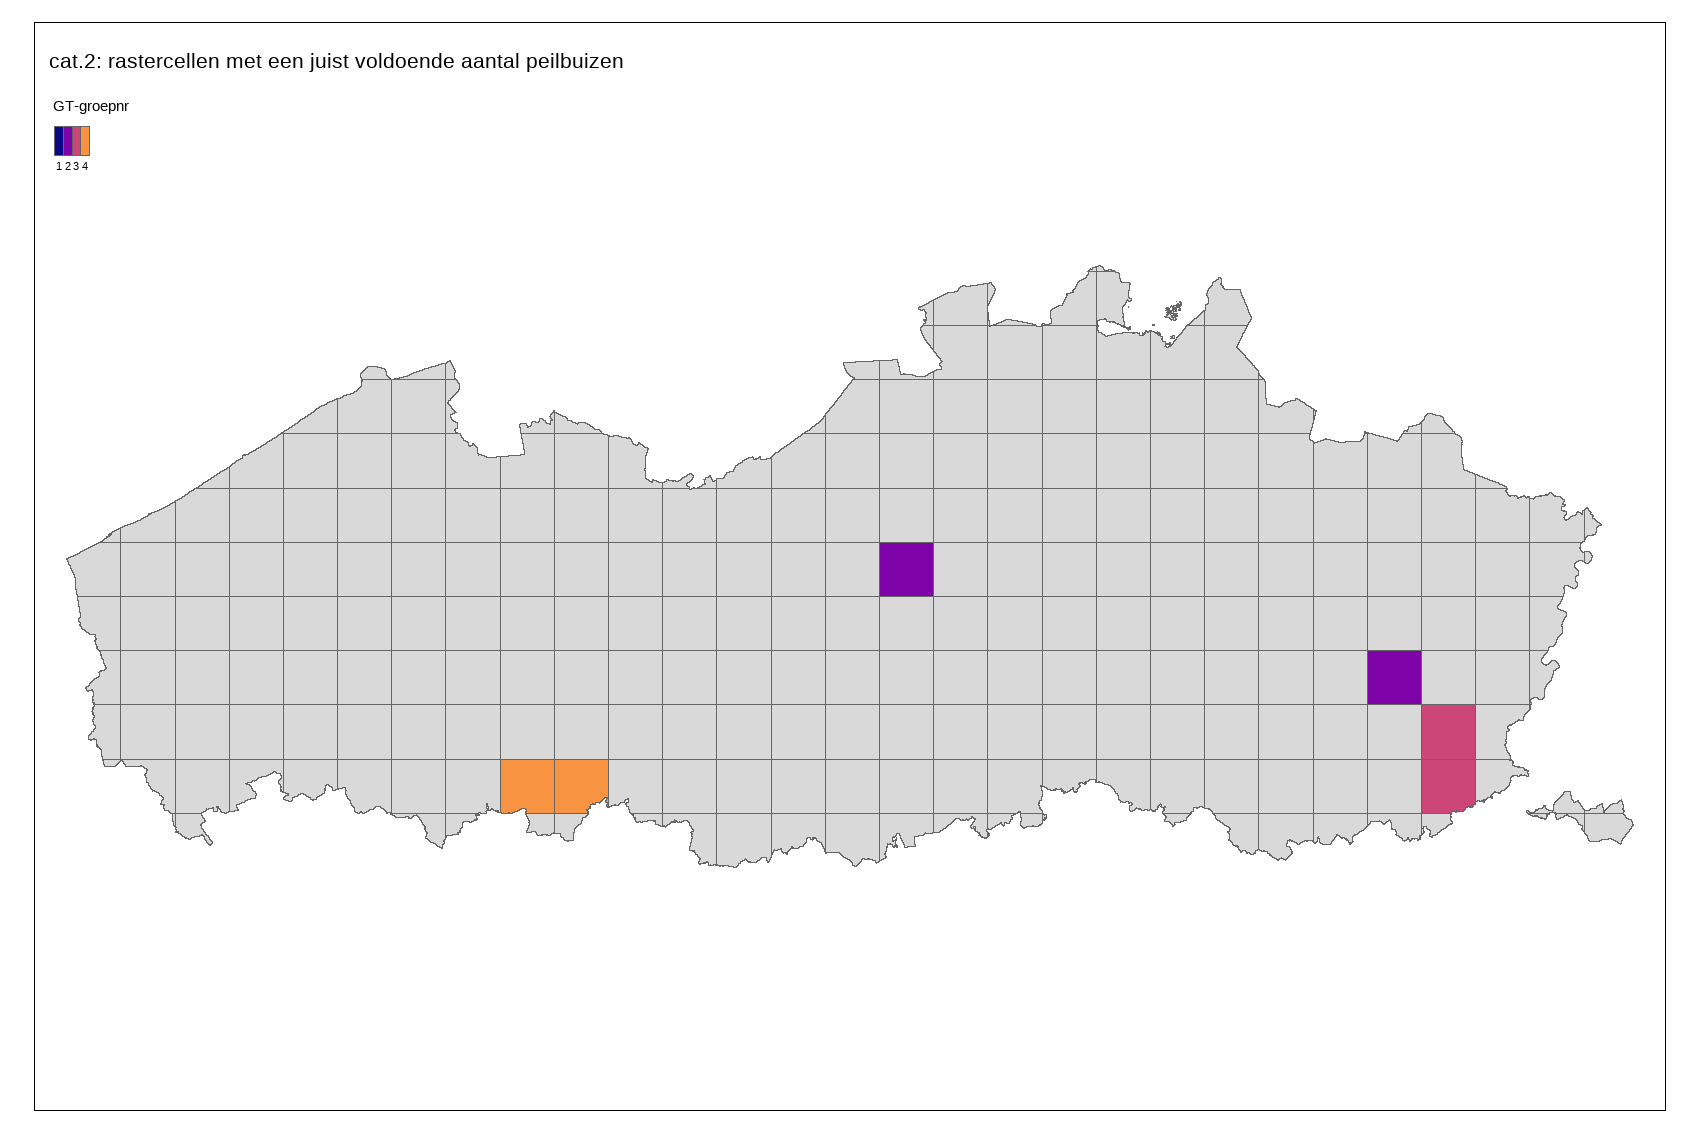
\includegraphics{droogtemeetnet_ontwerp_files/figure-latex/cat2-plot-1.pdf}
\caption{\label{fig:cat2-plot}rastercellen met een juist voldoende aantal
peilbuizen}
\end{figure}

\subsection{Categorie 3: Rastercellen met een overschot aan
peilbuizen}\label{cat3}

De rastercellen van categorie 3 bevatten meer meetlocaties
(Watina-peilbuizen) dan er voor het droogtemeetnet gezocht worden. Het
zijn in feite de resterende cellen, cellen die niet tot een van de
vorige categorieën behoren.

Hier geven we een overzicht over welke rastercellen het gaat (tabel
\ref{tab:cat3-table})

\begin{table}

\caption{\label{tab:cat3-table}Categorie 3: rastercellen met een overaanbod van peilbuizen}
\centering
\begin{tabular}[t]{r|r|r|r|r|r|r}
\hline
rastercelnummer & GTgroep & gewenst \# meetptn & \# peilbuizen & rang spreiding & rang lengte tijdreeks & rang combi\\
\hline
1 & 5 & 1 & 8 & 1 & 1 & 1\\
\hline
41 & 2 & 1 & 2 & 1 & 1 & 1\\
\hline
46 & 5 & 1 & 3 & 1 & 1 & 1\\
\hline
53 & 5 & 1 & 2 & 1 & 1 & 1\\
\hline
54 & 2 & 1 & 9 & 1 & 1 & 1\\
\hline
54 & 3 & 1 & 3 & 1 & 1 & 1\\
\hline
57 & 4 & 1 & 2 & 1 & 1 & 1\\
\hline
89 & 4 & 1 & 1 & 1 & 1 & 1\\
\hline
113 & 5 & 1 & 3 & 1 & 1 & 1\\
\hline
118 & 1 & 1 & 1 & 1 & 1 & 1\\
\hline
134 & 1 & 1 & 4 & 1 & 1 & 1\\
\hline
134 & 4 & 1 & 3 & 1 & 1 & 1\\
\hline
146 & 1 & 1 & 2 & 1 & 1 & 1\\
\hline
166 & 2 & 1 & 3 & 1 & 1 & 1\\
\hline
177 & 4 & 1 & 16 & 1 & 1 & 1\\
\hline
177 & 5 & 1 & 11 & 1 & 1 & 1\\
\hline
185 & 4 & 1 & 2 & 1 & 1 & 1\\
\hline
198 & 4 & 1 & 1 & 1 & 1 & 1\\
\hline
210 & 3 & 1 & 2 & 1 & 1 & 1\\
\hline
217 & 3 & 1 & 2 & 1 & 1 & 1\\
\hline
217 & 4 & 1 & 3 & 1 & 1 & 1\\
\hline
262 & 2 & 1 & 2 & 1 & 1 & 1\\
\hline
262 & 3 & 1 & 1 & 1 & 1 & 1\\
\hline
262 & 4 & 1 & 1 & 1 & 1 & 1\\
\hline
274 & 2 & 1 & 1 & 1 & 1 & 1\\
\hline
306 & 1 & 1 & 4 & 1 & 1 & 1\\
\hline
309 & 5 & 1 & 6 & 1 & 1 & 1\\
\hline
310 & 2 & 1 & 6 & 1 & 1 & 1\\
\hline
310 & 3 & 1 & 1 & 1 & 1 & 1\\
\hline
342 & 1 & 1 & 4 & 1 & 1 & 1\\
\hline
390 & 4 & 1 & 8 & 1 & 1 & 1\\
\hline
437 & 5 & 1 & 4 & 1 & 1 & 1\\
\hline
438 & 2 & 1 & 4 & 1 & 1 & 1\\
\hline
438 & 3 & 1 & 1 & 1 & 1 & 1\\
\hline
454 & 4 & 1 & 5 & 1 & 1 & 1\\
\hline
470 & 1 & 1 & 1 & 1 & 1 & 1\\
\hline
478 & 3 & 1 & 1 & 1 & 1 & 1\\
\hline
486 & 2 & 1 & 1 & 1 & 1 & 1\\
\hline
565 & 1 & 1 & 7 & 1 & 1 & 1\\
\hline
582 & 4 & 1 & 1 & 1 & 1 & 1\\
\hline
601 & 4 & 1 & 3 & 1 & 1 & 1\\
\hline
630 & 1 & 1 & 3 & 1 & 1 & 1\\
\hline
630 & 3 & 1 & 5 & 1 & 1 & 1\\
\hline
693 & 2 & 1 & 2 & 1 & 1 & 1\\
\hline
693 & 3 & 1 & 8 & 1 & 1 & 1\\
\hline
693 & 5 & 1 & 8 & 1 & 1 & 1\\
\hline
694 & 1 & 1 & 4 & 1 & 1 & 1\\
\hline
694 & 3 & 1 & 2 & 1 & 1 & 1\\
\hline
710 & 4 & 1 & 2 & 1 & 1 & 1\\
\hline
722 & 1 & 1 & 6 & 1 & 1 & 1\\
\hline
722 & 3 & 1 & 5 & 1 & 1 & 1\\
\hline
734 & 3 & 1 & 4 & 1 & 1 & 1\\
\hline
734 & 5 & 1 & 4 & 1 & 1 & 1\\
\hline
745 & 3 & 2 & 2 & 1 & 1 & 1\\
\hline
817 & 4 & 1 & 14 & 1 & 1 & 1\\
\hline
817 & 5 & 1 & 3 & 1 & 1 & 1\\
\hline
822 & 1 & 1 & 8 & 1 & 1 & 1\\
\hline
822 & 3 & 1 & 8 & 1 & 1 & 1\\
\hline
850 & 1 & 1 & 1 & 1 & 1 & 1\\
\hline
886 & 1 & 1 & 4 & 1 & 1 & 1\\
\hline
886 & 2 & 1 & 4 & 1 & 1 & 1\\
\hline
886 & 3 & 1 & 13 & 1 & 1 & 1\\
\hline
918 & 1 & 1 & 1 & 1 & 1 & 1\\
\hline
950 & 1 & 2 & 6 & 1 & 1 & 1\\
\hline
950 & 3 & 1 & 2 & 1 & 1 & 1\\
\hline
950 & 5 & 1 & 1 & 1 & 1 & 1\\
\hline
985 & 4 & 1 & 2 & 1 & 1 & 1\\
\hline
1010 & 1 & 1 & 3 & 1 & 1 & 1\\
\hline
1014 & 1 & 1 & 1 & 1 & 1 & 1\\
\hline
1017 & 3 & 1 & 3 & 1 & 1 & 1\\
\hline
\end{tabular}
\end{table}

Er zijn 72 gewenste meetlocaties waaraan meerdere peilbuizen kunnen
gelinkt worden. Ze zijn ruimtelijk goed verspreid over 70 rastercellen
(figuur \ref{fig:cat3-plot}).

\begin{figure}
\centering
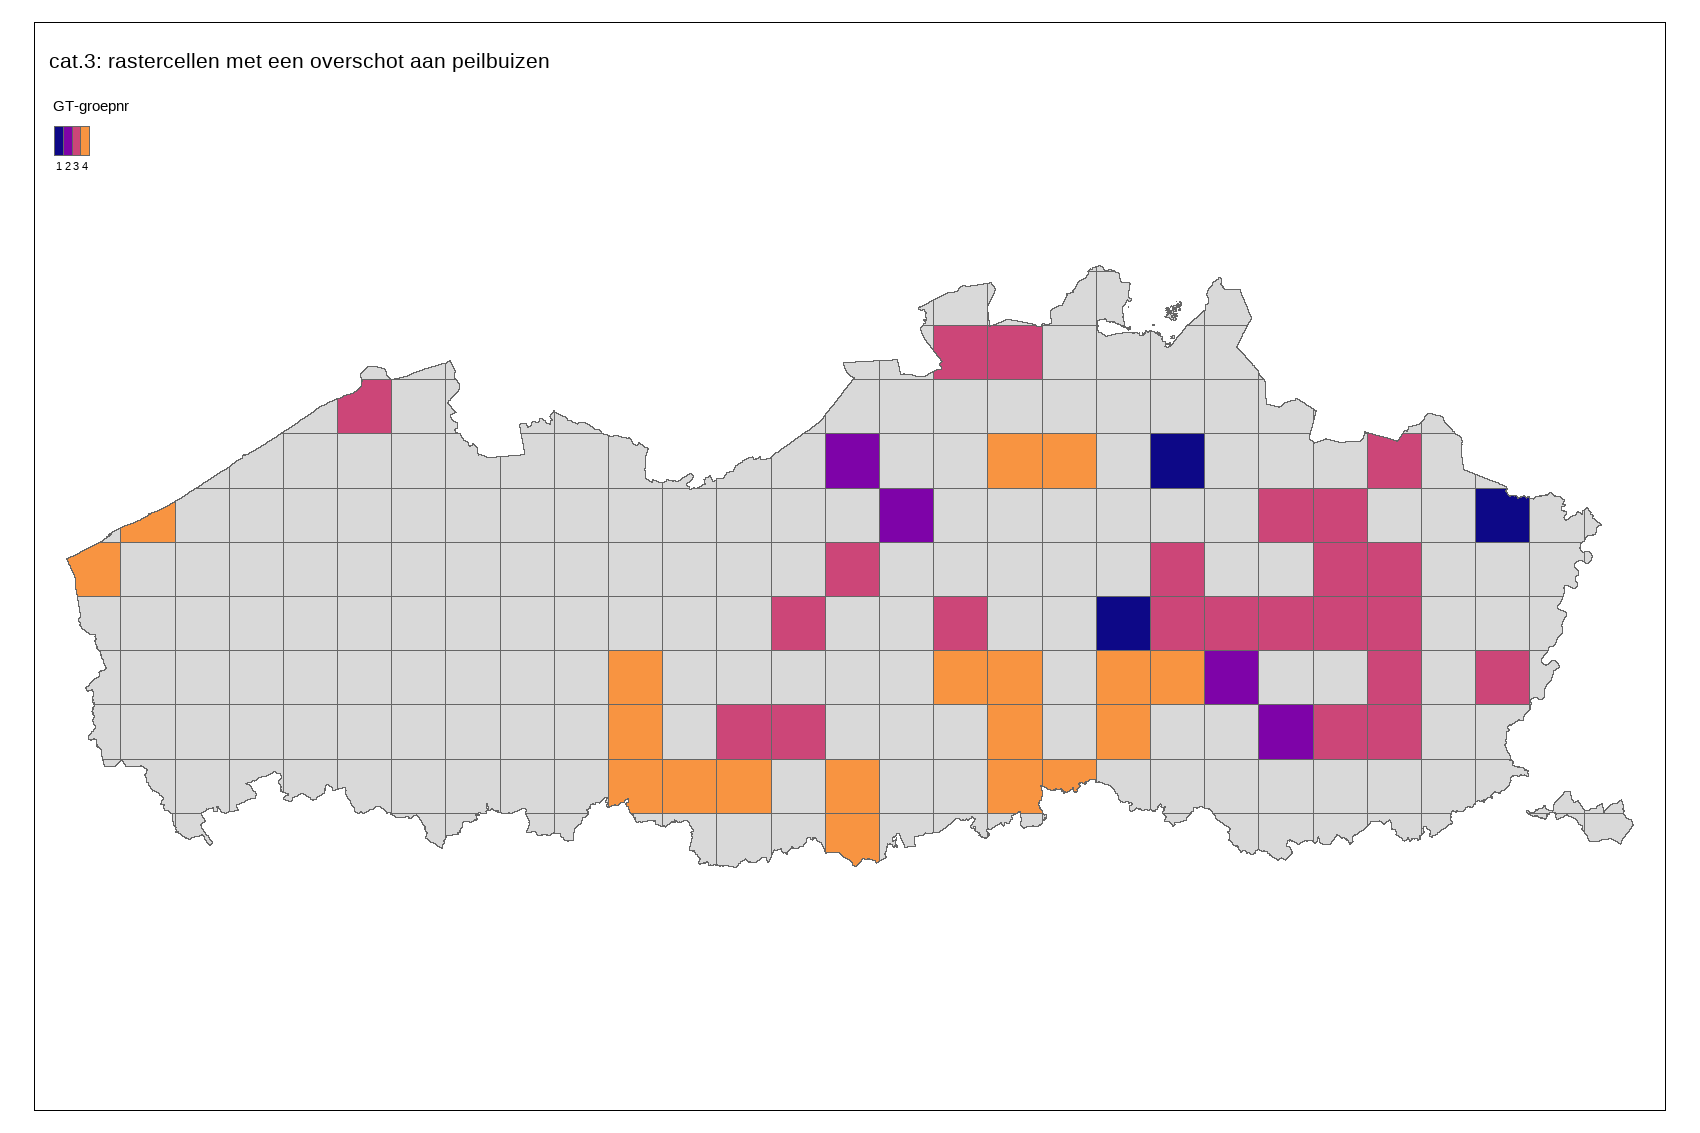
\includegraphics{droogtemeetnet_ontwerp_files/figure-latex/cat3-plot-1.pdf}
\caption{\label{fig:cat3-plot}rastercellen met een overschot aan peilbuizen}
\end{figure}

\subsubsection{Opzoeken van peilbuizen voor
tijdreeksanalyse}\label{opzoeken-pb}

Rastercellen van de drie categorieën kunnen peilbuizen bevatten die
verder met Menyanthes geanalyseerd gaan worden. In tabel
\ref{tab:tubes-cat123} wordt een overzicht gegeven van de desbetreffende
peilbuizen.

\begin{table}

\caption{\label{tab:tubes-cat123}Watina-meetpunten geselecteerd voor tijdreeksanalyse}
\centering
\begin{tabular}[t]{l|l|r|r|r|r}
\hline
watinacode & gebied & aantal jaren met lg3 & eerste lg3-jaar & recentste lg3-jaar & categorie\\
\hline
ALMP001 & Aalmoezenijbos / Aelmoeseneiebos / Gontrodebos & 3 & 2004 & 2006 & 3\\
\hline
ALMP002 & Aalmoezenijbos / Aelmoeseneiebos / Gontrodebos & 5 & 2004 & 2008 & 3\\
\hline
ALMP003 & Aalmoezenijbos / Aelmoeseneiebos / Gontrodebos & 5 & 2004 & 2008 & 3\\
\hline
ASBP001 & Asbeek & 9 & 2008 & 2016 & 3\\
\hline
BELP004 & de Belv<e9>d<e8>re & 5 & 2001 & 2006 & 3\\
\hline
BELP005 & de Belv<e9>d<e8>re & 5 & 2001 & 2006 & 3\\
\hline
BELP006 & de Belv<e9>d<e8>re & 5 & 2001 & 2006 & 3\\
\hline
BELP008 & de Belv<e9>d<e8>re & 5 & 2001 & 2006 & 3\\
\hline
BELP009 & de Belv<e9>d<e8>re & 5 & 2001 & 2006 & 3\\
\hline
BELP010 & de Belv<e9>d<e8>re & 5 & 2001 & 2006 & 3\\
\hline
BOBP018 & Bosbeekvallei & 3 & 2012 & 2014 & 3\\
\hline
BREP201 & Bredene - De Haan & 1 & 2009 & 2009 & 3\\
\hline
BREP202 & Bredene - De Haan & 1 & 2009 & 2009 & 3\\
\hline
BREP203 & Bredene - De Haan & 1 & 2009 & 2009 & 3\\
\hline
BREP204 & Bredene - De Haan & 1 & 2009 & 2009 & 3\\
\hline
BREP205 & Bredene - De Haan & 1 & 2009 & 2009 & 3\\
\hline
BREP206 & Bredene - De Haan & 1 & 2009 & 2009 & 3\\
\hline
BREP207 & Bredene - De Haan & 1 & 2009 & 2009 & 3\\
\hline
BREP210 & Bredene - De Haan & 1 & 2009 & 2009 & 3\\
\hline
BREP216 & Bredene - De Haan & 1 & 2009 & 2009 & 3\\
\hline
BRSP008 & Domeinbos Brasschaat (Inslag) & 0 & NA & NA & 1\\
\hline
BTRP001 & Bos ter Rijst & 1 & 2003 & 2003 & 2\\
\hline
BUIP021 & Buitengoor & 5 & 2008 & 2015 & 3\\
\hline
CABP303 & Cabourduinen & 4 & 2005 & 2008 & 3\\
\hline
COOP001 & Coolhembos & 8 & 2006 & 2015 & 2\\
\hline
DORP024 & Dorent & 3 & 2005 & 2014 & 3\\
\hline
DPBP007 & Diepenbeek & 0 & NA & NA & 2\\
\hline
DUNP010 & Dunbergbroek & 6 & 2004 & 2013 & 3\\
\hline
DUNP011 & Dunbergbroek & 4 & 2007 & 2016 & 3\\
\hline
DUNP012 & Dunbergbroek & 6 & 2004 & 2013 & 3\\
\hline
DYLP029 & Dijlevallei & 5 & 2004 & 2016 & 3\\
\hline
DYLP037 & Dijlevallei & 10 & 2004 & 2016 & 3\\
\hline
DYLP109 & Dijlevallei & 10 & 2004 & 2016 & 3\\
\hline
DYLP156 & Dijlevallei & 1 & 2016 & 2016 & 3\\
\hline
GOBP004 & Gorenbroek & 3 & 2014 & 2016 & 3\\
\hline
GROP001 & Grotenhoutbos & 0 & NA & NA & 3\\
\hline
GROP002 & Grotenhoutbos & 0 & NA & NA & 3\\
\hline
GSCP021 & Groot Schietveld & 3 & 2001 & 2010 & 3\\
\hline
HAGP019 & Hageven & 14 & 2002 & 2015 & 3\\
\hline
HALP002 & Hallerbos & 8 & 2008 & 2015 & 3\\
\hline
HALP005 & Hallerbos & 5 & 2008 & 2012 & 3\\
\hline
HBTP007 & Helderbeekvallei Terril & 2 & 2011 & 2014 & 3\\
\hline
HBTP008 & Helderbeekvallei Terril & 2 & 2011 & 2014 & 3\\
\hline
HEIP005 & Heist & 0 & NA & NA & 3\\
\hline
HOSP041 & Houtsaegerduinen/oosthoek & 1 & 2006 & 2006 & 3\\
\hline
HOSP088 & Houtsaegerduinen/oosthoek & 2 & 2005 & 2006 & 3\\
\hline
ITTP212 & Itterbeekvallei & 5 & 2012 & 2016 & 3\\
\hline
KALP022 & Kalmthoutse heide & 3 & 2014 & 2016 & 3\\
\hline
KALP136 & Kalmthoutse heide & 5 & 2011 & 2015 & 3\\
\hline
KALP137 & Kalmthoutse heide & 5 & 2011 & 2015 & 3\\
\hline
KALP252 & Kalmthoutse heide & 3 & 2014 & 2016 & 3\\
\hline
KALP316 & Kalmthoutse heide & 0 & NA & NA & 3\\
\hline
KALP319 & Kalmthoutse heide & 0 & NA & NA & 3\\
\hline
KALP327 & Kalmthoutse heide & 0 & NA & NA & 3\\
\hline
KALP357 & Kalmthoutse heide & 0 & NA & NA & 3\\
\hline
KBRP060 & Potpolder Kruibeke Rupelmonde & 11 & 2001 & 2012 & 2\\
\hline
LAVP080 & Laanvallei & 2 & 2011 & 2012 & 3\\
\hline
LDOP019 & Langdonken & 8 & 2004 & 2012 & 3\\
\hline
LDOP035 & Langdonken & 9 & 2005 & 2016 & 3\\
\hline
LDOP036 & Langdonken & 6 & 2005 & 2012 & 3\\
\hline
LDOP041 & Langdonken & 10 & 2005 & 2016 & 3\\
\hline
LDOP042 & Langdonken & 6 & 2007 & 2016 & 3\\
\hline
LEPP009 & Lenspolder & 6 & 2004 & 2013 & 3\\
\hline
LEPP011 & Lenspolder & 6 & 2004 & 2013 & 3\\
\hline
MANP029 & Mangelbeekvallei & 6 & 2008 & 2016 & 3\\
\hline
MATP003 & De Maten & 5 & 2011 & 2016 & 3\\
\hline
MATP010 & De Maten & 5 & 2012 & 2016 & 3\\
\hline
MATP013 & De Maten & 5 & 2012 & 2016 & 3\\
\hline
MATP015 & De Maten & 5 & 2012 & 2016 & 3\\
\hline
MECP050 & Mechelse Heide & 10 & 2007 & 2016 & 3\\
\hline
MOGP003 & Mosselgoren & 0 & NA & NA & 2\\
\hline
MOLP018 & Molenbeekvallei & 9 & 2001 & 2013 & 3\\
\hline
MOLP022 & Molenbeekvallei & 9 & 2001 & 2013 & 3\\
\hline
MOLP023 & Molenbeekvallei & 9 & 2001 & 2013 & 3\\
\hline
MOLP024 & Molenbeekvallei & 9 & 2001 & 2013 & 3\\
\hline
MOLP025 & Molenbeekvallei & 9 & 2001 & 2013 & 3\\
\hline
MOSP001 & De Most & 9 & 2006 & 2014 & 3\\
\hline
MOSP003 & De Most & 9 & 2006 & 2014 & 3\\
\hline
MOSP004 & De Most & 9 & 2006 & 2014 & 3\\
\hline
MSBP001 & Molenstedebroek & 0 & NA & NA & 3\\
\hline
MSBP002 & Molenstedebroek & 0 & NA & NA & 3\\
\hline
MSBP003 & Molenstedebroek & 0 & NA & NA & 3\\
\hline
MSBP006 & Molenstedebroek & 0 & NA & NA & 3\\
\hline
MSBP007 & Molenstedebroek & 0 & NA & NA & 3\\
\hline
MSBP008 & Molenstedebroek & 0 & NA & NA & 3\\
\hline
MSBP009 & Molenstedebroek & 0 & NA & NA & 3\\
\hline
MSBP013 & Molenstedebroek & 0 & NA & NA & 3\\
\hline
MSBP014 & Molenstedebroek & 0 & NA & NA & 3\\
\hline
NEIP001 & Neigembos & 4 & 2007 & 2010 & 3\\
\hline
NEIP002 & Neigembos & 4 & 2007 & 2010 & 3\\
\hline
NODP004 & Noordduinen & 5 & 2002 & 2006 & 3\\
\hline
NODP006 & Noordduinen & 5 & 2002 & 2006 & 3\\
\hline
NUCP004 & De Nuchten & 1 & 2008 & 2008 & 3\\
\hline
NUCP005 & De Nuchten & 1 & 2008 & 2008 & 3\\
\hline
ORCP002 & De Orchis & 2 & 2001 & 2002 & 3\\
\hline
ORCP003 & De Orchis & 2 & 2001 & 2002 & 3\\
\hline
OSKP026 & Oostends krekengebied & 5 & 2003 & 2009 & 3\\
\hline
OSKP038 & Oostends krekengebied & 5 & 2003 & 2009 & 3\\
\hline
PARP002 & Parike-bos & 2 & 2009 & 2010 & 3\\
\hline
PARP003 & Parike-bos & 4 & 2009 & 2012 & 3\\
\hline
RASP001 & Raspaillebos & 2 & 2003 & 2009 & 3\\
\hline
RASP002 & Raspaillebos & 3 & 2003 & 2012 & 3\\
\hline
RASP003 & Raspaillebos & 3 & 2003 & 2012 & 3\\
\hline
ROTP003 & Rotbroek & 3 & 2014 & 2016 & 3\\
\hline
SANP006 & Schansbeemden & 0 & NA & NA & 3\\
\hline
SBBP002 & Steenbergse bossen & 1 & 2003 & 2003 & 3\\
\hline
SBEP001 & Schuddebeurze & 12 & 2001 & 2012 & 3\\
\hline
SCPP021 & Scheps & 7 & 2008 & 2014 & 3\\
\hline
SCPP024 & Scheps & 7 & 2006 & 2012 & 3\\
\hline
SCPP025 & Scheps & 6 & 2006 & 2011 & 3\\
\hline
SCPP027 & Scheps & 5 & 2007 & 2012 & 3\\
\hline
SCPP033 & Scheps & 7 & 2008 & 2014 & 3\\
\hline
SCPP034 & Scheps & 7 & 2008 & 2014 & 3\\
\hline
SCPP035 & Scheps & 7 & 2008 & 2014 & 3\\
\hline
SCPP036 & Scheps & 7 & 2008 & 2014 & 3\\
\hline
SCPP039 & Scheps & 7 & 2008 & 2014 & 3\\
\hline
SCPP040 & Scheps & 7 & 2008 & 2014 & 3\\
\hline
SCPP042 & Scheps & 7 & 2008 & 2014 & 3\\
\hline
SCPP043 & Scheps & 7 & 2008 & 2014 & 3\\
\hline
SCPP045 & Scheps & 8 & 2004 & 2014 & 3\\
\hline
SCPP047 & Scheps & 6 & 2008 & 2014 & 3\\
\hline
SCPP050 & Scheps & 7 & 2008 & 2014 & 3\\
\hline
SCPP051 & Scheps & 4 & 2011 & 2014 & 3\\
\hline
SHHP031 & Schietveld Houthalen Hechteren & 5 & 2009 & 2016 & 3\\
\hline
SHHP032 & Schietveld Houthalen Hechteren & 7 & 2008 & 2016 & 3\\
\hline
SNOP022 & Snoekengracht & 0 & NA & NA & 3\\
\hline
SNOP025 & Snoekengracht & 0 & NA & NA & 3\\
\hline
SNOP028 & Snoekengracht & 0 & NA & NA & 3\\
\hline
SNOP029 & Snoekengracht & 0 & NA & NA & 3\\
\hline
SNOP031 & Snoekengracht & 0 & NA & NA & 3\\
\hline
SNOP032 & Snoekengracht & 0 & NA & NA & 3\\
\hline
SNOP033 & Snoekengracht & 0 & NA & NA & 3\\
\hline
SNOP129 & Snoekengracht & 0 & NA & NA & 3\\
\hline
STAP050 & Stamprooierbroek incl de Zig \& & 9 & 2001 & 2016 & 3\\
\hline
SWPP032 & Scheldemeersen Wortegem-Petege & 1 & 2010 & 2010 & 2\\
\hline
TEUP019 & De Teut & 5 & 2010 & 2014 & 3\\
\hline
TEUP026 & De Teut & 9 & 2008 & 2016 & 3\\
\hline
TEUP028 & De Teut & 6 & 2008 & 2016 & 3\\
\hline
TEUP043 & De Teut & 10 & 2007 & 2016 & 3\\
\hline
TEUP044 & De Teut & 9 & 2008 & 2016 & 3\\
\hline
TEUP045 & De Teut & 7 & 2008 & 2014 & 3\\
\hline
TEUP046 & De Teut & 7 & 2008 & 2016 & 3\\
\hline
TEUP047 & De Teut & 9 & 2008 & 2016 & 3\\
\hline
TIEP013 & Militair domein Tielen & 1 & 2006 & 2006 & 3\\
\hline
TLAP001 & Terlaemen \& Weijerman & 0 & NA & NA & 3\\
\hline
TLAP002 & Terlaemen \& Weijerman & 0 & NA & NA & 3\\
\hline
TLAP003 & Terlaemen \& Weijerman & 0 & NA & NA & 3\\
\hline
TORP018 & Torfbroek & 12 & 2005 & 2016 & 3\\
\hline
TVGP043 & Turnhouts Vennengebied & 0 & NA & NA & 3\\
\hline
TYDP004 & Ter Yde & 7 & 2004 & 2012 & 3\\
\hline
TYDP012 & Ter Yde & 8 & 2004 & 2012 & 3\\
\hline
TYDP031 & Ter Yde & 8 & 2004 & 2012 & 3\\
\hline
TYDP050 & Ter Yde & 10 & 2001 & 2012 & 3\\
\hline
TYDP055 & Ter Yde & 10 & 2001 & 2012 & 3\\
\hline
TYDP057 & Ter Yde & 10 & 2001 & 2012 & 3\\
\hline
TYDP058 & Ter Yde & 10 & 2001 & 2012 & 3\\
\hline
TYDP059 & Ter Yde & 9 & 2001 & 2010 & 3\\
\hline
TYDP072 & Ter Yde & 9 & 2001 & 2010 & 3\\
\hline
TYDP203 & Ter Yde & 6 & 2005 & 2012 & 3\\
\hline
TYDP204 & Ter Yde & 7 & 2005 & 2012 & 3\\
\hline
TYDP206 & Ter Yde & 7 & 2005 & 2012 & 3\\
\hline
TYDP207 & Ter Yde & 7 & 2005 & 2012 & 3\\
\hline
TYDP211 & Ter Yde & 6 & 2006 & 2012 & 3\\
\hline
UKPP010 & Uitkerkse Polder & 0 & NA & NA & 3\\
\hline
UKPP018 & Uitkerkse Polder & 0 & NA & NA & 3\\
\hline
UKPP022 & Uitkerkse Polder & 0 & NA & NA & 3\\
\hline
UKPP024 & Uitkerkse Polder & 0 & NA & NA & 3\\
\hline
UKPP027 & Uitkerkse Polder & 0 & NA & NA & 3\\
\hline
UKPP030 & Uitkerkse Polder & 0 & NA & NA & 3\\
\hline
UKPP032 & Uitkerkse Polder & 0 & NA & NA & 3\\
\hline
UKPP033 & Uitkerkse Polder & 0 & NA & NA & 3\\
\hline
UKPP034 & Uitkerkse Polder & 0 & NA & NA & 3\\
\hline
UKPP039 & Uitkerkse Polder & 0 & NA & NA & 3\\
\hline
UKPP041 & Uitkerkse Polder & 0 & NA & NA & 3\\
\hline
VDBP018 & Vallei van de Drie Beken & 3 & 2006 & 2015 & 3\\
\hline
VDBP024 & Vallei van de Drie Beken & 4 & 2006 & 2016 & 3\\
\hline
VDBP025 & Vallei van de Drie Beken & 4 & 2006 & 2016 & 3\\
\hline
VDBP034 & Vallei van de Drie Beken & 4 & 2006 & 2016 & 3\\
\hline
VDBP062 & Vallei van de Drie Beken & 4 & 2006 & 2016 & 3\\
\hline
VDBP503 & Vallei van de Drie Beken & 2 & 2006 & 2014 & 3\\
\hline
VDBP514 & Vallei van de Drie Beken & 5 & 2006 & 2016 & 3\\
\hline
VDBP531 & Vallei van de Drie Beken & 4 & 2006 & 2016 & 3\\
\hline
VENP005 & De Vennen & 5 & 2012 & 2016 & 3\\
\hline
VENP006 & De Vennen & 5 & 2012 & 2016 & 3\\
\hline
VENP009 & De Vennen & 5 & 2012 & 2016 & 3\\
\hline
VENP010 & De Vennen & 5 & 2012 & 2016 & 3\\
\hline
VENP012 & De Vennen & 4 & 2012 & 2015 & 3\\
\hline
VIEP104 & Vierkensbroek-Demervallei & 1 & 2003 & 2003 & 3\\
\hline
VIEP105 & Vierkensbroek-Demervallei & 3 & 2001 & 2003 & 3\\
\hline
VIEP106 & Vierkensbroek-Demervallei & 1 & 2001 & 2001 & 3\\
\hline
VIEP107 & Vierkensbroek-Demervallei & 2 & 2001 & 2002 & 3\\
\hline
VIEP173 & Vierkensbroek-Demervallei & 2 & 2001 & 2002 & 3\\
\hline
VIEP174 & Vierkensbroek-Demervallei & 2 & 2002 & 2003 & 3\\
\hline
VINP084 & Het Vinne & 1 & 2005 & 2005 & 3\\
\hline
VISP015 & Visbeekvallei & 3 & 2002 & 2004 & 3\\
\hline
VOTP003 & Vorsdonkbos-Turfputten & 6 & 2007 & 2012 & 3\\
\hline
VOTP020 & Vorsdonkbos-Turfputten & 9 & 2007 & 2015 & 3\\
\hline
VOTP055 & Vorsdonkbos-Turfputten & 9 & 2007 & 2015 & 3\\
\hline
VRIP024 & Vrieselhof & 0 & NA & NA & 2\\
\hline
VRIP039 & Vrieselhof & 1 & 2009 & 2009 & 3\\
\hline
WAHP711 & Waaslandhaven & 2 & 2003 & 2007 & 3\\
\hline
WAHP712 & Waaslandhaven & 2 & 2003 & 2007 & 3\\
\hline
WALP005 & Walenbos & 0 & NA & NA & 2\\
\hline
WALP041 & Walenbos & 6 & 2006 & 2011 & 3\\
\hline
WEBP036 & Webbekomsbroek & 2 & 2012 & 2013 & 3\\
\hline
WELP018 & Wellemeersen & 0 & NA & NA & 3\\
\hline
WELP020 & Wellemeersen & 0 & NA & NA & 3\\
\hline
WELP022 & Wellemeersen & 0 & NA & NA & 3\\
\hline
WERP001 & De Werft & 3 & 2008 & 2011 & 3\\
\hline
WERP002 & De Werft & 3 & 2008 & 2011 & 3\\
\hline
WERP003 & De Werft & 3 & 2008 & 2011 & 3\\
\hline
WERP004 & De Werft & 3 & 2008 & 2011 & 3\\
\hline
WERP005 & De Werft & 3 & 2008 & 2011 & 3\\
\hline
WERP007 & De Werft & 3 & 2008 & 2011 & 3\\
\hline
WERP009 & De Werft & 3 & 2008 & 2011 & 3\\
\hline
WERP011 & De Werft & 3 & 2008 & 2011 & 3\\
\hline
WERP012 & De Werft & 2 & 2008 & 2009 & 3\\
\hline
WESP003 & Westhoek & 12 & 2001 & 2012 & 3\\
\hline
WESP005 & Westhoek & 12 & 2001 & 2012 & 3\\
\hline
WESP007 & Westhoek & 10 & 2003 & 2012 & 3\\
\hline
WESP008 & Westhoek & 12 & 2001 & 2012 & 3\\
\hline
WESP014 & Westhoek & 12 & 2001 & 2012 & 3\\
\hline
WESP018 & Westhoek & 11 & 2001 & 2012 & 3\\
\hline
WESP050 & Westhoek & 12 & 2001 & 2012 & 3\\
\hline
WESP057 & Westhoek & 12 & 2001 & 2012 & 3\\
\hline
WESP073 & Westhoek & 12 & 2001 & 2012 & 3\\
\hline
WESP074 & Westhoek & 12 & 2001 & 2012 & 3\\
\hline
WESP076 & Westhoek & 12 & 2001 & 2012 & 3\\
\hline
WESP080 & Westhoek & 12 & 2001 & 2012 & 3\\
\hline
WESP097 & Westhoek & 11 & 2002 & 2012 & 3\\
\hline
WESP111 & Westhoek & 11 & 2002 & 2012 & 3\\
\hline
WESP119 & Westhoek & 12 & 2001 & 2012 & 3\\
\hline
WESP134 & Westhoek & 9 & 2003 & 2012 & 3\\
\hline
ZABP003 & Zammelsbroek & 4 & 2001 & 2009 & 3\\
\hline
ZABP004 & Zammelsbroek & 3 & 2002 & 2009 & 3\\
\hline
ZABP005 & Zammelsbroek & 1 & 2009 & 2009 & 3\\
\hline
ZABP013 & Zammelsbroek & 1 & 2009 & 2009 & 3\\
\hline
ZABP014 & Zammelsbroek & 1 & 2009 & 2009 & 3\\
\hline
ZABP022 & Zammelsbroek & 1 & 2009 & 2009 & 3\\
\hline
ZABP023 & Zammelsbroek & 1 & 2009 & 2009 & 3\\
\hline
ZEBP001 & Zeebrugge & 1 & 2011 & 2011 & 3\\
\hline
ZEBP003 & Zeebrugge & 1 & 2011 & 2011 & 3\\
\hline
ZEBP005 & Zeebrugge & 1 & 2011 & 2011 & 3\\
\hline
ZEBP009 & Zeebrugge & 0 & NA & NA & 3\\
\hline
ZEBP012 & Zeebrugge & 1 & 2011 & 2011 & 3\\
\hline
ZEBP019 & Zeebrugge & 1 & 2011 & 2011 & 3\\
\hline
ZEBP025 & Zeebrugge & 1 & 2011 & 2011 & 3\\
\hline
ZEBP045 & Zeebrugge & 1 & 2014 & 2014 & 3\\
\hline
ZEBP046 & Zeebrugge & 1 & 2014 & 2014 & 3\\
\hline
ZEBP107 & Zeebrugge & 0 & NA & NA & 3\\
\hline
ZEMP005 & Zemst & 6 & 2005 & 2010 & 3\\
\hline
ZIEP003 & Ziepbeekvallei & 10 & 2006 & 2016 & 3\\
\hline
ZWAP141 & Zwarte Beek & 10 & 2007 & 2016 & 3\\
\hline
ZWAP165 & Zwarte Beek & 10 & 2007 & 2016 & 3\\
\hline
ZWAP196 & Zwarte Beek & 10 & 2007 & 2016 & 3\\
\hline
ZWAP200 & Zwarte Beek & 12 & 2005 & 2016 & 3\\
\hline
ZWAP202 & Zwarte Beek & 11 & 2004 & 2015 & 3\\
\hline
ZWAP208 & Zwarte Beek & 13 & 2004 & 2016 & 3\\
\hline
ZWAP216 & Zwarte Beek & 11 & 2004 & 2015 & 3\\
\hline
ZWAP228 & Zwarte Beek & 9 & 2004 & 2016 & 3\\
\hline
ZWAP229 & Zwarte Beek & 10 & 2007 & 2016 & 3\\
\hline
ZWAP234 & Zwarte Beek & 6 & 2008 & 2016 & 3\\
\hline
ZWAP241 & Zwarte Beek & 8 & 2009 & 2016 & 3\\
\hline
ZWAP300 & Zwarte Beek & 4 & 2013 & 2016 & 3\\
\hline
ZWAP301 & Zwarte Beek & 4 & 2013 & 2016 & 3\\
\hline
ZWAP303 & Zwarte Beek & 1 & 2015 & 2015 & 3\\
\hline
ZWAP305 & Zwarte Beek & 2 & 2015 & 2016 & 3\\
\hline
ZWAP306 & Zwarte Beek & 2 & 2015 & 2016 & 3\\
\hline
ZWIP007 & Zwinduinen en -polders & 10 & 2004 & 2013 & 3\\
\hline
ZWIP014 & Zwinduinen en -polders & 9 & 2004 & 2012 & 3\\
\hline
ZWIP033 & Zwinduinen en -polders & 11 & 2005 & 2015 & 3\\
\hline
ZWIP036 & Zwinduinen en -polders & 10 & 2005 & 2015 & 3\\
\hline
ZWIP041 & Zwinduinen en -polders & 10 & 2005 & 2015 & 3\\
\hline
ZWIP042 & Zwinduinen en -polders & 11 & 2005 & 2015 & 3\\
\hline
ZWIP104 & Zwinduinen en -polders & 0 & NA & NA & 3\\
\hline
ZWIP108 & Zwinduinen en -polders & 0 & NA & NA & 3\\
\hline
ZWIP204 & Zwinduinen en -polders & 0 & NA & NA & 3\\
\hline
ZWIP209 & Zwinduinen en -polders & 0 & NA & NA & 3\\
\hline
ZWIP210 & Zwinduinen en -polders & 0 & NA & NA & 3\\
\hline
ZWIP213 & Zwinduinen en -polders & 0 & NA & NA & 3\\
\hline
ZWIP217 & Zwinduinen en -polders & 0 & NA & NA & 3\\
\hline
ZWIP218 & Zwinduinen en -polders & 0 & NA & NA & 3\\
\hline
ZWIP220 & Zwinduinen en -polders & 0 & NA & NA & 3\\
\hline
\end{tabular}
\end{table}

\section{Tijdreeksanalyse}\label{tijdreeksanalyse_uitvoering}

Alle meetreeksen van de peilbuizen die behoren tot de geselecteerde
rastercellen van categorie 2 werden alle geïmporteerd in Menyanthes. Van
cat. 3 werden alleen de meetreeksen geïmporteerd van de beste clusters,
die toch ook al aanleiding gaven tot een overaanbod.

In Menyanthes werd een project opgezet met zoveel mogelijk verklarende
reeksen. Het betreft :

\begin{itemize}
\tightlist
\item
  297 tijdreeksen van neerslaggegevens, afkomstig van KMI (214
  stations), VMM (43 stations), KNMI (22 stations) en HIC (18 stations)
  en
\item
  20 tijdreeksen van evapotranspiratie, afkomstig van KMI (5 stations),
  KNMI (7 stations) en VMM (8 stations).
\end{itemize}

Bij de modelbouw werd steeds ook een versie met een lineaire trend
berekend waarvan de significantie werd onderzocht (zie
\protect\hyperlink{lintrend}{lineaire trend}).

\begin{table}

\caption{\label{tab:read-results-menyanthes}Overzicht resultaten tijdreeksanalyse}
\centering
\begin{tabular}[t]{l|r}
\hline
uitspraak & aantal\\
\hline
niet weerhouden, expertoordeel & 12\\
\hline
niet weerhouden, te korte tijdreeks & 138\\
\hline
niet weerhouden, te lage modelfit & 107\\
\hline
niet weerhouden, trend & 61\\
\hline
weerhouden & 183\\
\hline
weerhouden, expertoordeel & 12\\
\hline
\end{tabular}
\end{table}

Tabel \ref{tab:read-results-menyanthes} geeft per categorie een synthese
van de tijdreeksanalyse.

Van de 513 onderzochte meetreeksen werden in totaal 195 meetreeksen
weerhouden oftewel 38\%.

Het grootste deel (85\%) van meetpunten die beoordeeld werden met
expertoordeel (zijnde 31\%) werd afgekeurd door een te gering aantal
beschikbare peilmetingen.

\section{De rastercellen hercategoriseren na de
tijdreeksanalysen}\label{de-rastercellen-hercategoriseren-na-de-tijdreeksanalysen}

De resultaten van de tijdreeksanalysen dienen om de peilbuizen te
herevalueren. Het kan ook een doorwerking op de categorie-indeling van
de rastercellen hebben.

\subsection{Categorie 1: Zijn er rastercellen met onvoldoende
peilbuizen?}\label{categorie-1-zijn-er-rastercellen-met-onvoldoende-peilbuizen-1}

Deze categorie bleef onveranderd.

\subsection{Categorie 2: Rastercellen met een juist voldoend aantal
peilbuizen}\label{cat2}

Tabel \ref{tab:tubes-cat2-bis} toont de 8 peilbuizen die, na de
tijdreeksanalyse, nog tot de 8 rastercellen van deze categorie horen.

Figuur \ref{fig:cat2-plot-bis} toont de ligging ervan.

\begin{figure}
\centering
\includegraphics{droogtemeetnet_ontwerp_files/figure-latex/cat2-plot-bis-1.pdf}
\caption{\label{fig:cat2-plot-bis}rastercellen met een juist voldoende
aantal peilbuizen}
\end{figure}

\begin{table}

\caption{\label{tab:tubes-cat2-bis}Geselecteerde peilbuizen die behoren tot rastercellen van cat. 2}
\centering
\begin{tabular}[t]{r|r|l}
\hline
rastercelnummer & GTgroep & watinacode\\
\hline
25 & 4 & BTRP001\\
\hline
134 & 5 & WALP005\\
\hline
233 & 1 & COOP001\\
\hline
233 & 2 & KBRP060\\
\hline
306 & 2 & DPBP007\\
\hline
537 & 4 & SWPP032\\
\hline
758 & 1 & MOGP003\\
\hline
918 & 5 & VRIP024\\
\hline
\end{tabular}
\end{table}

\subsection{Categorie 3: Rastercellen met een overschot aan
peilbuizen}\label{cat3}

De overige 70 rastercellen, categorie 3, bevatten meer meetlocaties
(Watina-peilbuizen) dan er voor het droogtemeetnet gezocht worden.

Figuur \ref{fig:cat3-plot-bis} toont de spreiding ervan. De rastercellen
liggen goed gespreid over Vlaanderen. Het is echter opvallend dat de
verschillende GT-groepen waartoe ze behoren daarentegen vrij geclusterd
voorkomen. Groepen 1 en 3 komen vooral in de Kempen voor. Rastercellen
van groep 4 ligt alle in de (zand)leemstreek\footnote{Dit is normaal,
  omdat alle cellen van deze groep in de (zand)leemstreek liggen.} en
deze van groep 5 liggen uitsluitend in de duinstreek.

\begin{figure}
\centering
\includegraphics{droogtemeetnet_ontwerp_files/figure-latex/cat3-plot-bis-1.pdf}
\caption{\label{fig:cat3-plot-bis}rastercellen met een overschot aan
peilbuizen}
\end{figure}

\subsubsection{Opzoeken van peilbuizen voor de rastercellen van cat.
3}\label{opzoeken-van-peilbuizen-voor-de-rastercellen-van-cat.-3}

Tabel \ref{tab:tubes-cat3-bis} geeft het resultaat van deze analyse.

\begin{table}

\caption{\label{tab:tubes-cat3-bis}Peilbuizen die behoren tot rastercellen van cat. 3}
\centering
\begin{tabular}[t]{l|r|r|r}
\hline
watinacode & aantal jaren met lg3 & eerste lg3-jaar & recentste lg3-jaar\\
\hline
SWEP004 & 100 & NA & 2019\\
\hline
WAHP711 & 0 & 2003 & 0\\
\hline
WAHP712 & 0 & 2003 & 0\\
\hline
TVGP043 & 100 & NA & 2019\\
\hline
ZWIP104 & 0 & NA & 0\\
\hline
ZWIP108 & 0 & NA & 0\\
\hline
MSBP001 & 0 & NA & 0\\
\hline
MSBP002 & 0 & NA & 0\\
\hline
MSBP003 & 0 & NA & 0\\
\hline
MSBP006 & 0 & NA & 0\\
\hline
MSBP007 & 0 & NA & 0\\
\hline
MSBP008 & 0 & NA & 0\\
\hline
MSBP009 & 0 & NA & 0\\
\hline
MSBP013 & 0 & NA & 0\\
\hline
MSBP014 & 0 & NA & 0\\
\hline
VDBP004 & 100 & NA & 2019\\
\hline
VDBP513 & 100 & NA & 2019\\
\hline
VDBP531 & 100 & 2006 & 2019\\
\hline
WEBP210 & 100 & 2009 & 2019\\
\hline
NEIP001 & 0 & 2007 & 0\\
\hline
NEIP002 & 0 & 2007 & 0\\
\hline
BOEP003 & 0 & NA & 0\\
\hline
SBBP002 & 0 & 2003 & 0\\
\hline
ZWBP013 & 0 & NA & 0\\
\hline
ZWBP014 & 0 & NA & 0\\
\hline
ZWBP017 & 0 & NA & 0\\
\hline
OSKP038 & 100 & 2003 & 2019\\
\hline
BUIP011 & 100 & 2001 & 2019\\
\hline
BUIP015 & 100 & 2001 & 2019\\
\hline
BUIP023 & 100 & 2001 & 2019\\
\hline
BUIP027 & 100 & 2001 & 2019\\
\hline
BUIP032 & 100 & 2001 & 2019\\
\hline
BUIP033 & 100 & 2001 & 2019\\
\hline
VOTP055 & 100 & 2007 & 2019\\
\hline
DUNP010 & 100 & 2004 & 2019\\
\hline
DUNP012 & 100 & 2004 & 2019\\
\hline
ITTP212 & 100 & 2012 & 2019\\
\hline
GOBP004 & 100 & 2014 & 2019\\
\hline
ROTP003 & 100 & 2014 & 2019\\
\hline
WEBP036 & 100 & 2012 & 2019\\
\hline
WEBP202 & 100 & NA & 2019\\
\hline
WESP002 & 100 & 2002 & 2019\\
\hline
WESP003 & 100 & 2001 & 2019\\
\hline
WESP005 & 100 & 2001 & 2019\\
\hline
WESP007 & 100 & 2003 & 2019\\
\hline
WESP008 & 100 & 2001 & 2019\\
\hline
WESP014 & 100 & 2001 & 2019\\
\hline
WESP018 & 100 & 2001 & 2019\\
\hline
WESP093 & 100 & 2001 & 2019\\
\hline
WESP097 & 100 & 2002 & 2019\\
\hline
WESP111 & 100 & 2002 & 2019\\
\hline
WESP119 & 100 & 2001 & 2019\\
\hline
WESP134 & 100 & 2003 & 2019\\
\hline
WESP302 & 100 & 2003 & 2019\\
\hline
BELP004 & 100 & 2001 & 2019\\
\hline
BELP010 & 100 & 2001 & 2019\\
\hline
NODP006 & 100 & 2002 & 2019\\
\hline
HALP001 & 0 & NA & 0\\
\hline
HALP002 & 0 & 2008 & 0\\
\hline
HALP005 & 0 & 2008 & 0\\
\hline
TORP018 & 100 & 2005 & 2019\\
\hline
SHHP035 & 100 & 2011 & 2019\\
\hline
ZWAP231 & 100 & 2008 & 2019\\
\hline
MOEP011 & 100 & NA & 2019\\
\hline
MOEP030 & 100 & 2003 & 2019\\
\hline
KLUP003 & 0 & 2003 & 0\\
\hline
RASP001 & 0 & 2003 & 0\\
\hline
RASP002 & 0 & 2003 & 0\\
\hline
RASP003 & 0 & 2003 & 0\\
\hline
DYLP029 & 100 & 2004 & 2019\\
\hline
LAVP080 & 100 & 2011 & 2019\\
\hline
DYLP020 & 100 & 2004 & 2019\\
\hline
DYLP021 & 100 & 2004 & 2019\\
\hline
DYLP066 & 100 & 2004 & 2019\\
\hline
DYLP071 & 100 & 2004 & 2019\\
\hline
DYLP072 & 100 & 2004 & 2019\\
\hline
DYLP073 & 100 & 2004 & 2019\\
\hline
DYLP156 & 100 & 2016 & 2019\\
\hline
IJSP003 & 100 & 2001 & 2019\\
\hline
LAVP059 & 100 & 2001 & 2019\\
\hline
LAVP060 & 100 & 2001 & 2019\\
\hline
IJSP023 & 100 & 2006 & 2019\\
\hline
HAGP019 & 100 & 2002 & 2019\\
\hline
MATP003 & 100 & 2011 & 2019\\
\hline
MATP010 & 100 & 2012 & 2019\\
\hline
MATP015 & 100 & 2012 & 2019\\
\hline
ZWIP014 & 100 & 2004 & 2019\\
\hline
ZWIP033 & 100 & 2005 & 2019\\
\hline
ZWIP041 & 100 & 2005 & 2019\\
\hline
ZWIP042 & 100 & 2005 & 2019\\
\hline
VIEP104 & 0 & 2003 & 0\\
\hline
VIEP105 & 0 & 2001 & 0\\
\hline
VIEP106 & 0 & 2001 & 0\\
\hline
VIEP107 & 0 & 2001 & 0\\
\hline
VIEP117 & 0 & NA & 0\\
\hline
VIEP118 & 0 & NA & 0\\
\hline
VIEP173 & 0 & 2001 & 0\\
\hline
VIEP174 & 0 & 2002 & 0\\
\hline
LDOP041 & 100 & 2005 & 2019\\
\hline
LDOP019 & 100 & 2004 & 2019\\
\hline
LDOP035 & 100 & 2005 & 2019\\
\hline
SNOP022 & 100 & NA & 2019\\
\hline
SNOP025 & 100 & NA & 2019\\
\hline
SNOP028 & 100 & NA & 2019\\
\hline
SNOP029 & 100 & NA & 2019\\
\hline
SNOP031 & 100 & NA & 2019\\
\hline
SNOP032 & 100 & NA & 2019\\
\hline
SNOP129 & 100 & NA & 2019\\
\hline
UKPP018 & 100 & NA & 2019\\
\hline
VDBP514 & 100 & 2006 & 2019\\
\hline
VDBP018 & 100 & 2006 & 2019\\
\hline
VDBP506 & 100 & NA & 2019\\
\hline
ZWAP332 & 100 & NA & 2019\\
\hline
ZWAP335 & 100 & NA & 2019\\
\hline
MOLP018 & 100 & 2001 & 2019\\
\hline
MOLP023 & 100 & 2001 & 2019\\
\hline
MOLP024 & 100 & 2001 & 2019\\
\hline
MOLP025 & 100 & 2001 & 2019\\
\hline
VISP002 & 100 & NA & 2019\\
\hline
VISP015 & 100 & 2002 & 2019\\
\hline
VISP017 & 100 & NA & 2019\\
\hline
GSCP002 & 100 & 2001 & 2019\\
\hline
GSCP007 & 100 & 2001 & 2019\\
\hline
GSCP008 & 100 & NA & 2019\\
\hline
GSCP009 & 100 & 2001 & 2019\\
\hline
GSCP010 & 100 & 2001 & 2019\\
\hline
GSCP011 & 100 & 2001 & 2019\\
\hline
GSCP017 & 100 & 2001 & 2019\\
\hline
GSCP020 & 100 & 2001 & 2019\\
\hline
GSCP021 & 100 & 2001 & 2019\\
\hline
GSCP024 & 100 & NA & 2019\\
\hline
ARHP009 & 0 & NA & 0\\
\hline
ARHP010 & 0 & NA & 0\\
\hline
VINP044 & 0 & NA & 0\\
\hline
VINP084 & 0 & 2005 & 0\\
\hline
ZWIP204 & 0 & NA & 0\\
\hline
ZWIP209 & 0 & NA & 0\\
\hline
ZWIP210 & 0 & NA & 0\\
\hline
ZWIP213 & 0 & NA & 0\\
\hline
ZWIP217 & 0 & NA & 0\\
\hline
ZWIP218 & 0 & NA & 0\\
\hline
ZWIP220 & 0 & NA & 0\\
\hline
DYLP037 & 100 & 2004 & 2019\\
\hline
ALMP002 & 100 & 2004 & 2019\\
\hline
ALMP003 & 100 & 2004 & 2019\\
\hline
MOSP015 & 100 & 2015 & 2019\\
\hline
MOSP016 & 100 & 2015 & 2019\\
\hline
ZWAP304 & 100 & 2016 & 2019\\
\hline
ZWAP309 & 100 & 2015 & 2019\\
\hline
ZWAP300 & 100 & 2013 & 2019\\
\hline
ZWAP301 & 100 & 2013 & 2019\\
\hline
ZWAP303 & 100 & 2015 & 2019\\
\hline
ZWAP305 & 100 & 2015 & 2019\\
\hline
ZWAP306 & 100 & 2015 & 2019\\
\hline
ZEBP009 & 100 & NA & 2019\\
\hline
UKPP026 & 100 & NA & 2019\\
\hline
UKPP029 & 100 & NA & 2019\\
\hline
ZEBP046 & 100 & 2014 & 2019\\
\hline
UKPP024 & 100 & NA & 2019\\
\hline
UKPP030 & 100 & NA & 2019\\
\hline
UKPP032 & 100 & NA & 2019\\
\hline
UKPP033 & 100 & NA & 2019\\
\hline
UKPP034 & 100 & NA & 2019\\
\hline
UKPP039 & 100 & NA & 2019\\
\hline
SANP006 & 0 & NA & 0\\
\hline
TLAP001 & 0 & NA & 0\\
\hline
TLAP002 & 0 & NA & 0\\
\hline
TLAP003 & 0 & NA & 0\\
\hline
HBTP007 & 100 & 2011 & 2019\\
\hline
HBTP008 & 100 & 2011 & 2019\\
\hline
LAAP003 & 100 & NA & 2019\\
\hline
TLAP004 & 100 & NA & 2019\\
\hline
ZEMP005 & 100 & 2005 & 2019\\
\hline
TEUP043 & 100 & 2007 & 2019\\
\hline
TEUP045 & 100 & 2008 & 2019\\
\hline
KALP136 & 100 & 2011 & 2019\\
\hline
KALP319 & 100 & NA & 2019\\
\hline
ORCP002 & 100 & 2001 & 2019\\
\hline
ORCP003 & 100 & 2001 & 2019\\
\hline
ORCP011 & 100 & NA & 2019\\
\hline
ORCP012 & 100 & NA & 2019\\
\hline
ORCP013 & 100 & NA & 2019\\
\hline
TYDP004 & 100 & 2004 & 2019\\
\hline
TYDP012 & 100 & 2004 & 2019\\
\hline
TYDP055 & 100 & 2001 & 2019\\
\hline
TYDP058 & 100 & 2001 & 2019\\
\hline
TYDP059 & 100 & 2001 & 2019\\
\hline
TYDP071 & 100 & 2003 & 2019\\
\hline
TYDP072 & 100 & 2001 & 2019\\
\hline
TYDP203 & 100 & 2005 & 2019\\
\hline
TYDP204 & 100 & 2005 & 2019\\
\hline
TYDP206 & 100 & 2005 & 2019\\
\hline
TYDP031 & 100 & 2004 & 2019\\
\hline
TYDP050 & 100 & 2001 & 2019\\
\hline
DEMP007 & 100 & 2005 & 2019\\
\hline
DEMP011 & 100 & NA & 2019\\
\hline
WERP001 & 100 & 2008 & 2019\\
\hline
WERP002 & 100 & 2008 & 2019\\
\hline
WERP003 & 100 & 2008 & 2019\\
\hline
WERP004 & 100 & 2008 & 2019\\
\hline
WERP009 & 100 & 2008 & 2019\\
\hline
WERP011 & 100 & 2008 & 2019\\
\hline
WERP012 & 100 & 2008 & 2019\\
\hline
ZABP022 & 100 & 2009 & 2019\\
\hline
WERP005 & 100 & 2008 & 2019\\
\hline
WERP007 & 100 & 2008 & 2019\\
\hline
ZABP003 & 100 & 2001 & 2019\\
\hline
ZABP004 & 100 & 2002 & 2019\\
\hline
ZABP005 & 100 & 2009 & 2019\\
\hline
ZABP013 & 100 & 2009 & 2019\\
\hline
ZABP014 & 100 & 2009 & 2019\\
\hline
ZABP023 & 100 & 2009 & 2019\\
\hline
BOBP018 & 100 & 2012 & 2019\\
\hline
SCPP027 & 100 & 2007 & 2019\\
\hline
SCPP045 & 100 & 2004 & 2019\\
\hline
VENP005 & 100 & 2012 & 2019\\
\hline
SCPP025 & 100 & 2006 & 2019\\
\hline
SCPP036 & 100 & 2008 & 2019\\
\hline
SCPP039 & 100 & 2008 & 2019\\
\hline
SCPP042 & 100 & 2008 & 2019\\
\hline
SCPP050 & 100 & 2008 & 2019\\
\hline
VENP006 & 100 & 2012 & 2019\\
\hline
VENP009 & 100 & 2012 & 2019\\
\hline
VENP010 & 100 & 2012 & 2019\\
\hline
VRIP009 & 100 & NA & 2019\\
\hline
VRIP011 & 100 & NA & 2019\\
\hline
VRIP013 & 100 & NA & 2019\\
\hline
VRIP039 & 100 & 2009 & 2019\\
\hline
ZWAP141 & 100 & 2007 & 2019\\
\hline
ZWAP200 & 100 & 2005 & 2019\\
\hline
ZWAP208 & 100 & 2004 & 2019\\
\hline
ZWAP216 & 100 & 2004 & 2019\\
\hline
ZWAP228 & 100 & 2004 & 2019\\
\hline
ZWAP234 & 100 & 2008 & 2019\\
\hline
ZWAP144 & 100 & NA & 2019\\
\hline
PARP002 & 100 & 2009 & 2019\\
\hline
PARP003 & 100 & 2009 & 2019\\
\hline
ZIEP003 & 100 & 2006 & 2019\\
\hline
TIEP026 & 100 & NA & 2019\\
\hline
WELP018 & 0 & NA & 0\\
\hline
WELP020 & 0 & NA & 0\\
\hline
WELP022 & 0 & NA & 0\\
\hline
\end{tabular}
\end{table}

Het gaat nog over 242 peilbuizen.

Het effectief toewijzen van een Watina-peilbuis aan een meetlocatie
wordt in de volgende sectie behandeld.

\section{Moeten nog bijkomende meetreeksen geanalyseerd
worden?}\label{moeten-nog-bijkomende-meetreeksen-geanalyseerd-worden}

Door de tijdreeksanalyse kan het zijn dat meetreeksen met relatief veel
metingen toch niet weerhouden werden. Doordat niet op alle meetreeksen
van categorie 3 een tijdreeksanalyse werd uitgevoerd, kan het zijn dat
er hierdoor rastercellen zijn waarbij meetreeksen van een oorspronkelijk
lagere rang, nu wel de hoogste rang bekleden. De tijdreeks van deze
meetreeksen worden dan best eerst geanalyseerd, waarna een nieuwe
categorie-indeling volgt.

\begin{verbatim}
## Er hoeven geen bijkomende meetreeksen met Menyanthes onderzocht te worden.
\end{verbatim}

\section{Aanduiden van de
meetlocaties}\label{aanduiden-van-de-meetlocaties}

Het ontwerp van het meetnet moet resulteren in de aanduiding van een
aantal meetlocaties. Tot nog toe kennen we enkel voor de cat. 2 (tabel
\ref{tab:tubes-cat2-bis}) de exacte meetlocaties.

Voor cat. 1 moeten we nog uit alle geschikte habitatvlekken een vlek
kiezen en voor cat. 3 is nog een keuze te maken uit de peilbuizen.
Binnen categorie 3 wordt nog een onderscheid gemaakt of de peilbuizen
onmiddellijk (op vlak van datakwaliteit) in gebruik kunnen genomen
worden of niet. Deze keuzen worden in dit deel behandeld.

\subsection{Het toewijzen van een kandidaat peilbuis aan een
meetlocatie}\label{het-toewijzen-van-een-kandidaat-peilbuis-aan-een-meetlocatie}

Om uit verschillende gelijkwaardige kandidaat-peilbuizen er willekeurig
eentje uit te kiezen, maken we gebruik van het grts-raster (zie
\ref{sel-habvlek}). Een rastercel (8192 m x 8192 m) waarin meerdere
kandidaat peilbuizen liggen, wordt opgedeeld in mini-rastercellen van 32
m x 32 m. Elke mini-rastercel heeft een uniek rangnummer. De peilbuis
(of meerdere, gelijk aan het aantal gewenste meetlocaties) die in
rastercel met het/de laagste rangnummer(s) lig(gen), wordt dan effectief
geselecteerd. Indien in een rastercel voor meerdere GT-groepen naar een
meetlocatie gezocht wordt, herhaalt die procedure voor elke GT-groep
afzonderlijk.

Er is een routine geschreven die per rastercel en hierbinnen per
GT-groep deze klus klaart.

Figuur \ref{fig:tubes-excess-plot} geeft geografisch weer over welke
meetpunten en rasters het hier gaat. Er is hierbij een verschil gemaakt
tussen rasters waar een keuze uit peilbuizen van actueel lage kwaliteit
moet gemaakt worden en waar dit uit peilbuizen met modelleerbare
tijdreeksen kan. In een rastercel sluiten beide keuzen elkaar uit
wanneer er slechts één meetpunt gezocht wordt.

\begin{figure}
\centering
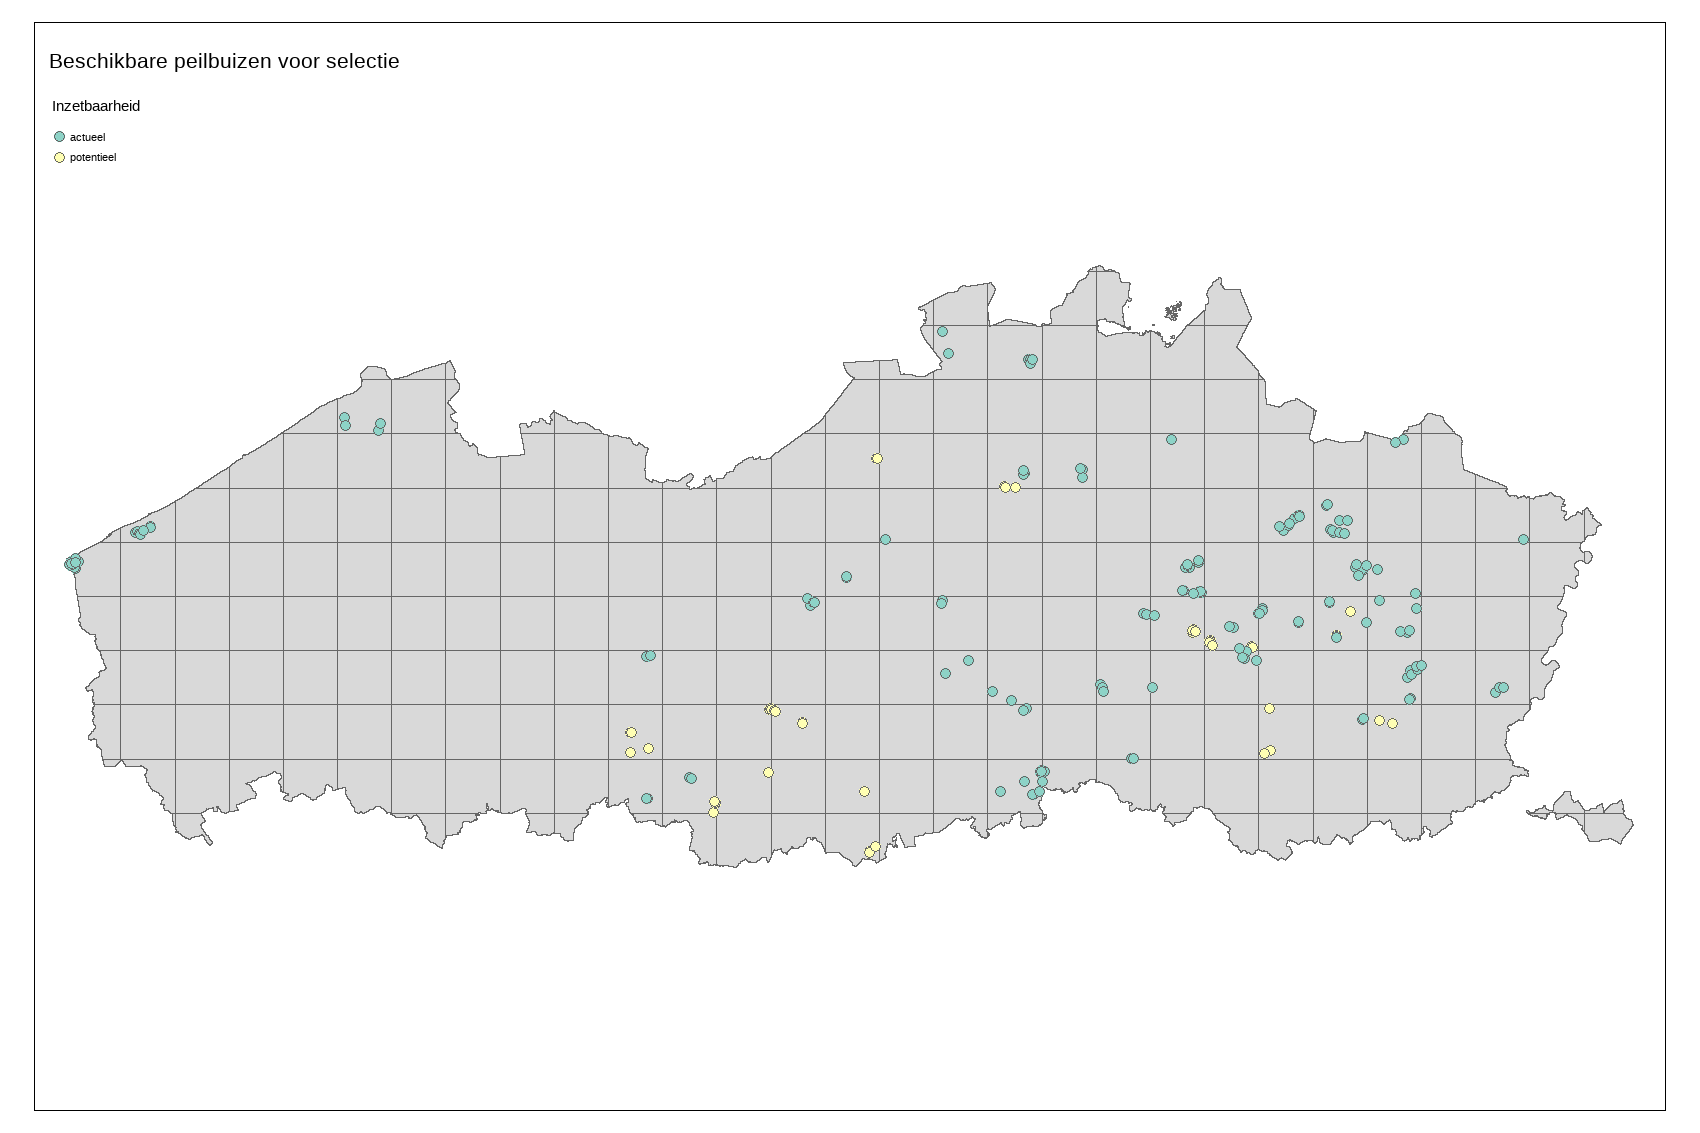
\includegraphics{droogtemeetnet_ontwerp_files/figure-latex/tubes-excess-plot-1.pdf}
\caption{\label{fig:tubes-excess-plot}de ligging van de beschikbare
peilbuizen}
\end{figure}

Tabel \ref{tab:grts-result-3-table} geeft het overzicht van de 72
geselecteerde meetpunten .

\begin{table}

\caption{\label{tab:grts-result-3-table}Geselecteerde peilbuizen die behoren tot rastercellen van cat. 3}
\centering
\begin{tabular}[t]{r|r|l|l|r|r}
\hline
rastercelnummer & GTgroep & gebied & watinacode & x & y\\
\hline
1 & 5 & Schorreweide & SWEP004 & 57388 & 213820\\
\hline
41 & 2 & Waaslandhaven & WAHP712 & 144656 & 214876\\
\hline
46 & 5 & Turnhouts Vennengebied & TVGP043 & 189364 & 226376\\
\hline
53 & 5 & Zwinduinen en -polders & ZWIP104 & 75551 & 226763\\
\hline
54 & 2 & Molenstedebroek & MSBP007 & 194938 & 187299\\
\hline
54 & 3 & Vallei van de Drie Beken & VDBP513 & 202202 & 191476\\
\hline
57 & 4 & Neigembos & NEIP001 & 128122 & 167393\\
\hline
89 & 4 & Boembeke & BOEP003 & 107334 & 170403\\
\hline
113 & 5 & Oostends krekengebied & OSKP038 & 54530 & 210938\\
\hline
118 & 1 & Buitengoor & BUIP027 & 206595 & 212155\\
\hline
134 & 1 & Vorsdonkbos-Turfputten & VOTP055 & 179763 & 184526\\
\hline
134 & 4 & Dunbergbroek & DUNP012 & 178707 & 179625\\
\hline
146 & 1 & Itterbeekvallei & ITTP212 & 242307 & 202672\\
\hline
166 & 2 & Rotbroek & ROTP003 & 200403 & 185618\\
\hline
177 & 4 & Westhoek & WESP008 & 22617 & 198715\\
\hline
177 & 5 & Noordduinen & NODP006 & 27875 & 200717\\
\hline
185 & 4 & Hallerbos & HALP001 & 143431 & 155389\\
\hline
198 & 4 & Torfbroek & TORP018 & 162023 & 179712\\
\hline
210 & 3 & Zwarte Beek & ZWAP231 & 220110 & 198031\\
\hline
217 & 3 & Moenebroeken & MOEP030 & 116473 & 166514\\
\hline
217 & 4 & Raspaillebos & RASP002 & 120111 & 162861\\
\hline
262 & 2 & Dijlevallei & DYLP029 & 169238 & 167404\\
\hline
262 & 3 & Laanvallei & LAVP059 & 168181 & 164052\\
\hline
262 & 4 & Ijsevallei & IJSP023 & 166813 & 166073\\
\hline
274 & 2 & Hageven & HAGP019 & 224064 & 217725\\
\hline
306 & 1 & De Maten & MATP010 & 225128 & 182769\\
\hline
309 & 5 & Zwinduinen en -polders & ZWIP041 & 77028 & 227941\\
\hline
310 & 2 & Vierkensbroek-Demervallei & VIEP117 & 192297 & 188970\\
\hline
310 & 3 & Langdonken & LDOP041 & 186424 & 191178\\
\hline
342 & 1 & Langdonken & LDOP019 & 184754 & 191421\\
\hline
390 & 4 & Snoekengracht & SNOP129 & 183331 & 169489\\
\hline
437 & 5 & Uitkerkse Polder & UKPP018 & 62808 & 222365\\
\hline
438 & 2 & Vallei van de Drie Beken & VDBP514 & 202304 & 191370\\
\hline
438 & 3 & Vallei van de Drie Beken & VDBP506 & 202732 & 191923\\
\hline
454 & 4 & Molenbeekvallei & MOLP023 & 166621 & 176753\\
\hline
470 & 1 & Visbeekvallei & VISP002 & 181212 & 217908\\
\hline
478 & 3 & Groot Schietveld & GSCP017 & 167657 & 229201\\
\hline
486 & 2 & Aronst Hoek & ARHP009 & 203834 & 177051\\
\hline
565 & 1 & Zwinduinen en -polders & ZWIP213 & 79544 & 228488\\
\hline
582 & 4 & Dijlevallei & DYLP037 & 169802 & 167510\\
\hline
601 & 4 & Aalmoezenijbos / Aelmoeseneiebos / Gontrodebos & ALMP003 & 110287 & 185136\\
\hline
630 & 1 & De Most & MOSP015 & 212551 & 207735\\
\hline
630 & 3 & Zwarte Beek & ZWAP303 & 213435 & 204022\\
\hline
693 & 2 & Zeebrugge & ZEBP009 & 69111 & 219114\\
\hline
693 & 3 & Uitkerkse Polder & UKPP029 & 64241 & 219799\\
\hline
693 & 5 & Uitkerkse Polder & UKPP039 & 63031 & 220174\\
\hline
694 & 1 & Terlaemen \& Weijerman & TLAP003 & 214025 & 187912\\
\hline
694 & 3 & Helderbeekvallei Terril & HBTP007 & 212987 & 193133\\
\hline
710 & 4 & Zemst & ZEMP005 & 158392 & 184259\\
\hline
722 & 1 & De Teut & TEUP043 & 223696 & 188700\\
\hline
722 & 3 & De Teut & TEUP045 & 225036 & 188792\\
\hline
734 & 3 & Kalmthoutse heide & KALP136 & 154423 & 234049\\
\hline
734 & 5 & Kalmthoutse heide & KALP319 & 155060 & 233988\\
\hline
745 & 3 & De Orchis & ORCP011 & 139864 & 196932\\
\hline
745 & 3 & De Orchis & ORCP012 & 139863 & 196973\\
\hline
817 & 4 & Ter Yde & TYDP204 & 33222 & 203448\\
\hline
817 & 5 & Ter Yde & TYDP050 & 32403 & 204128\\
\hline
822 & 1 & De Werft & WERP012 & 192332 & 194448\\
\hline
822 & 3 & Zammelsbroek & ZABP014 & 191421 & 198803\\
\hline
850 & 1 & Bosbeekvallei & BOBP018 & 240525 & 196690\\
\hline
886 & 1 & De Vennen & VENP005 & 208256 & 206362\\
\hline
886 & 2 & Scheps & SCPP025 & 206960 & 204244\\
\hline
886 & 3 & Scheps & SCPP042 & 205315 & 204593\\
\hline
918 & 1 & Vrieselhof & VRIP013 & 166733 & 212477\\
\hline
950 & 1 & Zwarte Beek & ZWAP141 & 216785 & 198435\\
\hline
950 & 1 & Zwarte Beek & ZWAP216 & 218514 & 198727\\
\hline
950 & 3 & Zwarte Beek & ZWAP228 & 217381 & 197149\\
\hline
950 & 5 & Zwarte Beek & ZWAP144 & 216583 & 198160\\
\hline
985 & 4 & Parike-bos & PARP003 & 109730 & 163542\\
\hline
1010 & 1 & Ziepbeekvallei & ZIEP003 & 238289 & 181160\\
\hline
1014 & 1 & Militair domein Tielen & TIEP026 & 189050 & 217720\\
\hline
1017 & 3 & Wellemeersen & WELP018 & 128284 & 176954\\
\hline
\end{tabular}
\end{table}

\subsection{Samenvatting selectie
peilbuizen}\label{samenvatting-selectie-peilbuizen}

Tabel \ref{tab:synthese-selection-tubes} toont het overzicht van alle 81
geselecteerde peilbuizen. Hiervan zijn er 66 die op basis van hun data
nu reeds inzetbaar zijn.

Tabel \ref{tab:synthese-reserve-tubes} geeft alle 157 reservepunten
weer.

\begin{table}

\caption{\label{tab:synthese-selection-tubes}Overzicht van de geselecteerde peilbuizen}
\centering
\begin{tabular}[t]{r|r|l|l|r|r|r|l}
\hline
rastercelnummer & GTgroep & gebied & watinacode & x & y & selectie & direct inzetbaar\\
\hline
1 & 5 & Schorreweide & SWEP004 & 57388 & 213820 & 1 & Ja\\
\hline
25 & 4 & Bos ter Rijst & BTRP001 & 101924 & 164018 & 1 & Ja\\
\hline
41 & 2 & Waaslandhaven & WAHP712 & 144656 & 214876 & -1 & Nee\\
\hline
46 & 5 & Turnhouts Vennengebied & TVGP043 & 189364 & 226376 & 1 & Ja\\
\hline
53 & 5 & Zwinduinen en -polders & ZWIP104 & 75551 & 226763 & -1 & Nee\\
\hline
54 & 2 & Molenstedebroek & MSBP007 & 194938 & 187299 & -1 & Nee\\
\hline
54 & 3 & Vallei van de Drie Beken & VDBP513 & 202202 & 191476 & 1 & Ja\\
\hline
57 & 4 & Neigembos & NEIP001 & 128122 & 167393 & -1 & Nee\\
\hline
89 & 4 & Boembeke & BOEP003 & 107334 & 170403 & -1 & Nee\\
\hline
113 & 5 & Oostends krekengebied & OSKP038 & 54530 & 210938 & 1 & Ja\\
\hline
118 & 1 & Buitengoor & BUIP027 & 206595 & 212155 & 1 & Ja\\
\hline
134 & 1 & Vorsdonkbos-Turfputten & VOTP055 & 179763 & 184526 & 1 & Ja\\
\hline
134 & 4 & Dunbergbroek & DUNP012 & 178707 & 179625 & 1 & Ja\\
\hline
134 & 5 & Walenbos & WALP005 & 184748 & 179727 & 1 & Ja\\
\hline
146 & 1 & Itterbeekvallei & ITTP212 & 242307 & 202672 & 1 & Ja\\
\hline
166 & 2 & Rotbroek & ROTP003 & 200403 & 185618 & 1 & Ja\\
\hline
177 & 4 & Westhoek & WESP008 & 22617 & 198715 & 1 & Ja\\
\hline
177 & 5 & Noordduinen & NODP006 & 27875 & 200717 & 1 & Ja\\
\hline
185 & 4 & Hallerbos & HALP001 & 143431 & 155389 & -1 & Nee\\
\hline
198 & 4 & Torfbroek & TORP018 & 162023 & 179712 & 1 & Ja\\
\hline
210 & 3 & Zwarte Beek & ZWAP231 & 220110 & 198031 & 1 & Ja\\
\hline
217 & 3 & Moenebroeken & MOEP030 & 116473 & 166514 & 1 & Ja\\
\hline
217 & 4 & Raspaillebos & RASP002 & 120111 & 162861 & -1 & Nee\\
\hline
233 & 1 & Coolhembos & COOP001 & 146113 & 196127 & 1 & Ja\\
\hline
233 & 2 & Potpolder Kruibeke Rupelmonde & KBRP060 & 145448 & 202168 & 1 & Ja\\
\hline
262 & 2 & Dijlevallei & DYLP029 & 169238 & 167404 & 1 & Ja\\
\hline
262 & 3 & Laanvallei & LAVP059 & 168181 & 164052 & 1 & Ja\\
\hline
262 & 4 & Ijsevallei & IJSP023 & 166813 & 166073 & 1 & Ja\\
\hline
274 & 2 & Hageven & HAGP019 & 224064 & 217725 & 1 & Ja\\
\hline
306 & 1 & De Maten & MATP010 & 225128 & 182769 & 1 & Ja\\
\hline
306 & 2 & Diepenbeek & DPBP007 & 221649 & 179772 & -1 & Nee\\
\hline
309 & 5 & Zwinduinen en -polders & ZWIP041 & 77028 & 227941 & 1 & Ja\\
\hline
310 & 2 & Vierkensbroek-Demervallei & VIEP117 & 192297 & 188970 & -1 & Nee\\
\hline
310 & 3 & Langdonken & LDOP041 & 186424 & 191178 & 1 & Ja\\
\hline
342 & 1 & Langdonken & LDOP019 & 184754 & 191421 & 1 & Ja\\
\hline
390 & 4 & Snoekengracht & SNOP129 & 183331 & 169489 & 1 & Ja\\
\hline
437 & 5 & Uitkerkse Polder & UKPP018 & 62808 & 222365 & 1 & Ja\\
\hline
438 & 2 & Vallei van de Drie Beken & VDBP514 & 202304 & 191370 & 1 & Ja\\
\hline
438 & 3 & Vallei van de Drie Beken & VDBP506 & 202732 & 191923 & 1 & Ja\\
\hline
454 & 4 & Molenbeekvallei & MOLP023 & 166621 & 176753 & 1 & Ja\\
\hline
470 & 1 & Visbeekvallei & VISP002 & 181212 & 217908 & 1 & Ja\\
\hline
478 & 3 & Groot Schietveld & GSCP017 & 167657 & 229201 & 1 & Ja\\
\hline
486 & 2 & Aronst Hoek & ARHP009 & 203834 & 177051 & -1 & Nee\\
\hline
537 & 4 & Scheldemeersen Wortegem-Petege & SWPP032 & 94675 & 169402 & 1 & Ja\\
\hline
565 & 1 & Zwinduinen en -polders & ZWIP213 & 79544 & 228488 & -1 & Nee\\
\hline
582 & 4 & Dijlevallei & DYLP037 & 169802 & 167510 & 1 & Ja\\
\hline
601 & 4 & Aalmoezenijbos / Aelmoeseneiebos / Gontrodebos & ALMP003 & 110287 & 185136 & 1 & Ja\\
\hline
630 & 1 & De Most & MOSP015 & 212551 & 207735 & 1 & Ja\\
\hline
630 & 3 & Zwarte Beek & ZWAP303 & 213435 & 204022 & 1 & Ja\\
\hline
693 & 2 & Zeebrugge & ZEBP009 & 69111 & 219114 & 1 & Ja\\
\hline
693 & 3 & Uitkerkse Polder & UKPP029 & 64241 & 219799 & 1 & Ja\\
\hline
693 & 5 & Uitkerkse Polder & UKPP039 & 63031 & 220174 & 1 & Ja\\
\hline
694 & 1 & Terlaemen \& Weijerman & TLAP003 & 214025 & 187912 & -1 & Nee\\
\hline
694 & 3 & Helderbeekvallei Terril & HBTP007 & 212987 & 193133 & 1 & Ja\\
\hline
710 & 4 & Zemst & ZEMP005 & 158392 & 184259 & 1 & Ja\\
\hline
722 & 1 & De Teut & TEUP043 & 223696 & 188700 & 1 & Ja\\
\hline
722 & 3 & De Teut & TEUP045 & 225036 & 188792 & 1 & Ja\\
\hline
734 & 3 & Kalmthoutse heide & KALP136 & 154423 & 234049 & 1 & Ja\\
\hline
734 & 5 & Kalmthoutse heide & KALP319 & 155060 & 233988 & 1 & Ja\\
\hline
745 & 3 & De Orchis & ORCP011 & 139864 & 196932 & 1 & Ja\\
\hline
745 & 3 & De Orchis & ORCP012 & 139863 & 196973 & 1 & Ja\\
\hline
758 & 1 & Mosselgoren & MOGP003 & 188983 & 208897 & -1 & Nee\\
\hline
817 & 4 & Ter Yde & TYDP204 & 33222 & 203448 & 1 & Ja\\
\hline
817 & 5 & Ter Yde & TYDP050 & 32403 & 204128 & 1 & Ja\\
\hline
822 & 1 & De Werft & WERP012 & 192332 & 194448 & 1 & Ja\\
\hline
822 & 3 & Zammelsbroek & ZABP014 & 191421 & 198803 & 1 & Ja\\
\hline
850 & 1 & Bosbeekvallei & BOBP018 & 240525 & 196690 & 1 & Ja\\
\hline
886 & 1 & De Vennen & VENP005 & 208256 & 206362 & 1 & Ja\\
\hline
886 & 2 & Scheps & SCPP025 & 206960 & 204244 & 1 & Ja\\
\hline
886 & 3 & Scheps & SCPP042 & 205315 & 204593 & 1 & Ja\\
\hline
918 & 1 & Vrieselhof & VRIP013 & 166733 & 212477 & 1 & Ja\\
\hline
918 & 5 & Vrieselhof & VRIP024 & 167122 & 212402 & 1 & Ja\\
\hline
950 & 1 & Zwarte Beek & ZWAP141 & 216785 & 198435 & 1 & Ja\\
\hline
950 & 1 & Zwarte Beek & ZWAP216 & 218514 & 198727 & 1 & Ja\\
\hline
950 & 3 & Zwarte Beek & ZWAP228 & 217381 & 197149 & 1 & Ja\\
\hline
950 & 5 & Zwarte Beek & ZWAP144 & 216583 & 198160 & 1 & Ja\\
\hline
985 & 4 & Parike-bos & PARP003 & 109730 & 163542 & 1 & Ja\\
\hline
990 & 5 & Domeinbos Brasschaat (Inslag) & BRSP008 & 160451 & 222061 & -1 & Nee\\
\hline
1010 & 1 & Ziepbeekvallei & ZIEP003 & 238289 & 181160 & 1 & Ja\\
\hline
1014 & 1 & Militair domein Tielen & TIEP026 & 189050 & 217720 & 1 & Ja\\
\hline
1017 & 3 & Wellemeersen & WELP018 & 128284 & 176954 & -1 & Nee\\
\hline
\end{tabular}
\end{table}

\begin{table}

\caption{\label{tab:synthese-reserve-tubes}Overzicht van de reserve peilbuizen}
\centering
\begin{tabular}[t]{r|r|l|l|r|r}
\hline
rastercelnummer & GTgroep & gebied & watinacode & x & y\\
\hline
41 & 2 & Waaslandhaven & WAHP711 & 144524 & 214863\\
\hline
53 & 5 & Zwinduinen en -polders & ZWIP108 & 75653 & 226501\\
\hline
54 & 2 & Molenstedebroek & MSBP003 & 194861 & 187151\\
\hline
54 & 2 & Molenstedebroek & MSBP002 & 194917 & 187270\\
\hline
54 & 2 & Molenstedebroek & MSBP013 & 195275 & 186651\\
\hline
54 & 2 & Molenstedebroek & MSBP009 & 194851 & 187121\\
\hline
54 & 2 & Molenstedebroek & MSBP014 & 195268 & 186601\\
\hline
54 & 2 & Molenstedebroek & MSBP008 & 194883 & 187199\\
\hline
54 & 2 & Molenstedebroek & MSBP006 & 194955 & 187335\\
\hline
54 & 3 & Vallei van de Drie Beken & VDBP004 & 198401 & 189278\\
\hline
54 & 3 & Vallei van de Drie Beken & VDBP531 & 197880 & 189431\\
\hline
54 & 3 & Webbekomsbroek & WEBP210 & 199320 & 186194\\
\hline
57 & 4 & Neigembos & NEIP002 & 128078 & 167410\\
\hline
89 & 4 & Zwalmbeek & ZWBP013 & 107282 & 173439\\
\hline
89 & 4 & Steenbergse bossen & SBBP002 & 109983 & 170962\\
\hline
89 & 4 & Zwalmbeek & ZWBP017 & 107421 & 173519\\
\hline
89 & 4 & Zwalmbeek & ZWBP014 & 107312 & 173473\\
\hline
118 & 1 & Buitengoor & BUIP023 & 206653 & 212114\\
\hline
118 & 1 & Buitengoor & BUIP015 & 206639 & 212165\\
\hline
118 & 1 & Buitengoor & BUIP033 & 206472 & 212059\\
\hline
134 & 4 & Dunbergbroek & DUNP010 & 178354 & 180655\\
\hline
166 & 2 & Webbekomsbroek & WEBP202 & 199709 & 184801\\
\hline
166 & 2 & Gorenbroek & GOBP004 & 201885 & 184397\\
\hline
166 & 2 & Webbekomsbroek & WEBP036 & 200108 & 184654\\
\hline
177 & 4 & Westhoek & WESP093 & 22509 & 198809\\
\hline
177 & 4 & Westhoek & WESP018 & 23813 & 199363\\
\hline
177 & 4 & Westhoek & WESP302 & 23338 & 199132\\
\hline
177 & 4 & Westhoek & WESP007 & 23034 & 198650\\
\hline
177 & 4 & Westhoek & WESP005 & 23086 & 198942\\
\hline
177 & 4 & Westhoek & WESP097 & 23408 & 198956\\
\hline
177 & 4 & Westhoek & WESP014 & 22737 & 199289\\
\hline
177 & 4 & Westhoek & WESP119 & 23171 & 198331\\
\hline
177 & 4 & Westhoek & WESP111 & 23304 & 198193\\
\hline
177 & 4 & Westhoek & WESP003 & 23288 & 198961\\
\hline
177 & 4 & Westhoek & WESP134 & 22885 & 198920\\
\hline
177 & 5 & de Belv<e9>d<e8>re & BELP010 & 27947 & 199669\\
\hline
177 & 5 & de Belv<e9>d<e8>re & BELP004 & 28016 & 199778\\
\hline
185 & 4 & Hallerbos & HALP005 & 144281 & 156162\\
\hline
185 & 4 & Hallerbos & HALP002 & 143429 & 155341\\
\hline
210 & 3 & Schietveld Houthalen Hechteren & SHHP035 & 225904 & 194393\\
\hline
217 & 3 & Moenebroeken & MOEP011 & 116115 & 166574\\
\hline
217 & 4 & Kluysbos & KLUP003 & 119864 & 161359\\
\hline
217 & 4 & Raspaillebos & RASP001 & 120085 & 162768\\
\hline
217 & 4 & Raspaillebos & RASP003 & 120002 & 163028\\
\hline
262 & 2 & Laanvallei & LAVP080 & 169110 & 164590\\
\hline
262 & 3 & Dijlevallei & DYLP021 & 169440 & 167581\\
\hline
262 & 3 & Ijsevallei & IJSP003 & 163141 & 164523\\
\hline
262 & 3 & Dijlevallei & DYLP020 & 169378 & 167510\\
\hline
262 & 3 & Laanvallei & LAVP060 & 168105 & 164098\\
\hline
262 & 3 & Dijlevallei & DYLP073 & 169323 & 167496\\
\hline
262 & 3 & Dijlevallei & DYLP066 & 169359 & 167629\\
\hline
262 & 3 & Dijlevallei & DYLP156 & 169478 & 166091\\
\hline
306 & 1 & De Maten & MATP003 & 224779 & 181757\\
\hline
306 & 1 & De Maten & MATP015 & 226040 & 183424\\
\hline
309 & 5 & Zwinduinen en -polders & ZWIP014 & 78202 & 228291\\
\hline
309 & 5 & Zwinduinen en -polders & ZWIP042 & 79233 & 228121\\
\hline
309 & 5 & Zwinduinen en -polders & ZWIP033 & 77640 & 228329\\
\hline
310 & 2 & Vierkensbroek-Demervallei & VIEP173 & 192713 & 188703\\
\hline
310 & 2 & Vierkensbroek-Demervallei & VIEP106 & 192282 & 188686\\
\hline
310 & 2 & Vierkensbroek-Demervallei & VIEP107 & 192278 & 188526\\
\hline
310 & 2 & Vierkensbroek-Demervallei & VIEP118 & 192266 & 188817\\
\hline
310 & 2 & Vierkensbroek-Demervallei & VIEP174 & 192711 & 188697\\
\hline
342 & 1 & Langdonken & LDOP035 & 185221 & 191291\\
\hline
390 & 4 & Snoekengracht & SNOP032 & 183056 & 169524\\
\hline
390 & 4 & Snoekengracht & SNOP029 & 183348 & 169465\\
\hline
390 & 4 & Snoekengracht & SNOP022 & 183102 & 169452\\
\hline
390 & 4 & Snoekengracht & SNOP031 & 183313 & 169446\\
\hline
390 & 4 & Snoekengracht & SNOP025 & 183238 & 169448\\
\hline
438 & 3 & Zwarte Beek & ZWAP335 & 208176 & 190160\\
\hline
438 & 3 & Zwarte Beek & ZWAP332 & 208201 & 190059\\
\hline
438 & 3 & Vallei van de Drie Beken & VDBP018 & 202838 & 192210\\
\hline
454 & 4 & Molenbeekvallei & MOLP018 & 167135 & 177145\\
\hline
454 & 4 & Molenbeekvallei & MOLP025 & 166664 & 176724\\
\hline
454 & 4 & Molenbeekvallei & MOLP024 & 166641 & 176739\\
\hline
470 & 1 & Visbeekvallei & VISP015 & 180942 & 217539\\
\hline
470 & 1 & Visbeekvallei & VISP017 & 181257 & 217859\\
\hline
478 & 3 & Groot Schietveld & GSCP007 & 167540 & 229836\\
\hline
478 & 3 & Groot Schietveld & GSCP011 & 167660 & 229863\\
\hline
478 & 3 & Groot Schietveld & GSCP020 & 167682 & 229188\\
\hline
478 & 3 & Groot Schietveld & GSCP002 & 167621 & 229841\\
\hline
478 & 3 & Groot Schietveld & GSCP008 & 167490 & 229826\\
\hline
478 & 3 & Groot Schietveld & GSCP024 & 168020 & 229769\\
\hline
478 & 3 & Groot Schietveld & GSCP021 & 167691 & 229182\\
\hline
478 & 3 & Groot Schietveld & GSCP009 & 167459 & 229809\\
\hline
486 & 2 & Het Vinne & VINP044 & 203993 & 170797\\
\hline
486 & 2 & Het Vinne & VINP084 & 203095 & 170251\\
\hline
486 & 2 & Aronst Hoek & ARHP010 & 203804 & 177070\\
\hline
565 & 1 & Zwinduinen en -polders & ZWIP217 & 79750 & 228352\\
\hline
565 & 1 & Zwinduinen en -polders & ZWIP210 & 80185 & 228761\\
\hline
565 & 1 & Zwinduinen en -polders & ZWIP218 & 80145 & 228399\\
\hline
565 & 1 & Zwinduinen en -polders & ZWIP209 & 79771 & 228690\\
\hline
565 & 1 & Zwinduinen en -polders & ZWIP204 & 79694 & 228868\\
\hline
565 & 1 & Zwinduinen en -polders & ZWIP220 & 79710 & 228136\\
\hline
601 & 4 & Aalmoezenijbos / Aelmoeseneiebos / Gontrodebos & ALMP002 & 109744 & 185010\\
\hline
630 & 1 & Zwarte Beek & ZWAP304 & 214442 & 205517\\
\hline
630 & 1 & De Most & MOSP016 & 212638 & 207858\\
\hline
630 & 1 & Zwarte Beek & ZWAP309 & 215657 & 205459\\
\hline
630 & 3 & Zwarte Beek & ZWAP306 & 215123 & 203590\\
\hline
630 & 3 & Zwarte Beek & ZWAP301 & 213467 & 203688\\
\hline
630 & 3 & Zwarte Beek & ZWAP305 & 214503 & 203705\\
\hline
630 & 3 & Zwarte Beek & ZWAP300 & 213086 & 204149\\
\hline
693 & 3 & Zeebrugge & ZEBP046 & 69422 & 220210\\
\hline
693 & 3 & Uitkerkse Polder & UKPP026 & 64020 & 221053\\
\hline
693 & 5 & Uitkerkse Polder & UKPP033 & 63326 & 220765\\
\hline
693 & 5 & Uitkerkse Polder & UKPP024 & 64131 & 220125\\
\hline
693 & 5 & Uitkerkse Polder & UKPP030 & 63295 & 219347\\
\hline
693 & 5 & Uitkerkse Polder & UKPP034 & 63040 & 221589\\
\hline
693 & 5 & Uitkerkse Polder & UKPP032 & 63399 & 220470\\
\hline
694 & 1 & Terlaemen \& Weijerman & TLAP001 & 213998 & 188072\\
\hline
694 & 1 & Schansbeemden & SANP006 & 216032 & 191815\\
\hline
694 & 3 & Laambroeken & LAAP003 & 218524 & 190066\\
\hline
694 & 3 & Terlaemen \& Weijerman & TLAP004 & 214019 & 187879\\
\hline
694 & 3 & Helderbeekvallei Terril & HBTP008 & 212972 & 193186\\
\hline
745 & 3 & De Orchis & ORCP013 & 139861 & 197002\\
\hline
817 & 4 & Ter Yde & TYDP203 & 33046 & 203477\\
\hline
817 & 4 & Ter Yde & TYDP004 & 33126 & 203530\\
\hline
817 & 4 & Ter Yde & TYDP055 & 32743 & 203672\\
\hline
817 & 4 & Ter Yde & TYDP071 & 33667 & 203943\\
\hline
817 & 4 & Ter Yde & TYDP059 & 32669 & 203788\\
\hline
817 & 4 & Ter Yde & TYDP206 & 33673 & 203910\\
\hline
817 & 4 & Ter Yde & TYDP072 & 33571 & 203880\\
\hline
817 & 4 & Ter Yde & TYDP012 & 33155 & 203402\\
\hline
817 & 4 & Ter Yde & TYDP058 & 32486 & 203672\\
\hline
817 & 5 & Ter Yde & TYDP031 & 33253 & 203328\\
\hline
822 & 1 & Zammelsbroek & ZABP022 & 193188 & 199206\\
\hline
822 & 1 & de Merode-Herselt & DEMP011 & 190657 & 194916\\
\hline
822 & 1 & de Merode-Herselt & DEMP007 & 190806 & 194941\\
\hline
822 & 1 & De Werft & WERP011 & 193419 & 194740\\
\hline
822 & 1 & De Werft & WERP001 & 193281 & 194778\\
\hline
822 & 1 & De Werft & WERP003 & 193271 & 194588\\
\hline
822 & 1 & De Werft & WERP004 & 193302 & 194696\\
\hline
822 & 1 & De Werft & WERP009 & 193488 & 194562\\
\hline
822 & 1 & De Werft & WERP002 & 193300 & 194752\\
\hline
822 & 3 & Zammelsbroek & ZABP013 & 191535 & 198711\\
\hline
822 & 3 & De Werft & WERP005 & 193360 & 194613\\
\hline
822 & 3 & Zammelsbroek & ZABP004 & 191712 & 198448\\
\hline
822 & 3 & Zammelsbroek & ZABP003 & 191644 & 198520\\
\hline
822 & 3 & De Werft & WERP007 & 193544 & 194610\\
\hline
822 & 3 & Zammelsbroek & ZABP023 & 193145 & 199376\\
\hline
822 & 3 & Zammelsbroek & ZABP005 & 191734 & 198418\\
\hline
886 & 1 & Scheps & SCPP045 & 206476 & 204589\\
\hline
886 & 1 & Scheps & SCPP027 & 205749 & 204186\\
\hline
886 & 3 & Scheps & SCPP036 & 205976 & 204000\\
\hline
886 & 3 & De Vennen & VENP010 & 208440 & 206098\\
\hline
886 & 3 & Scheps & SCPP050 & 207566 & 205767\\
\hline
886 & 3 & De Vennen & VENP009 & 208455 & 206286\\
\hline
886 & 3 & Scheps & SCPP039 & 206669 & 204706\\
\hline
886 & 3 & De Vennen & VENP006 & 208317 & 206290\\
\hline
918 & 1 & Vrieselhof & VRIP039 & 166653 & 213046\\
\hline
918 & 1 & Vrieselhof & VRIP009 & 166718 & 212654\\
\hline
918 & 1 & Vrieselhof & VRIP011 & 166854 & 212640\\
\hline
950 & 1 & Zwarte Beek & ZWAP208 & 218005 & 198226\\
\hline
950 & 1 & Zwarte Beek & ZWAP200 & 217985 & 197987\\
\hline
950 & 3 & Zwarte Beek & ZWAP234 & 217054 & 198920\\
\hline
985 & 4 & Parike-bos & PARP002 & 109810 & 163492\\
\hline
1017 & 3 & Wellemeersen & WELP022 & 128519 & 176887\\
\hline
1017 & 3 & Wellemeersen & WELP020 & 128401 & 177063\\
\hline
\end{tabular}
\end{table}

Figuur \ref{fig:tubes-selected-plot} toont de geselecteerde peilbuizen
op kaart. Er wordt een onderscheid gemaakt tussen de meetpunten die
meetpunten die reeds inzetbaar zijn en de meetpunten waarbij er nog
extra metingen nodig zijn.

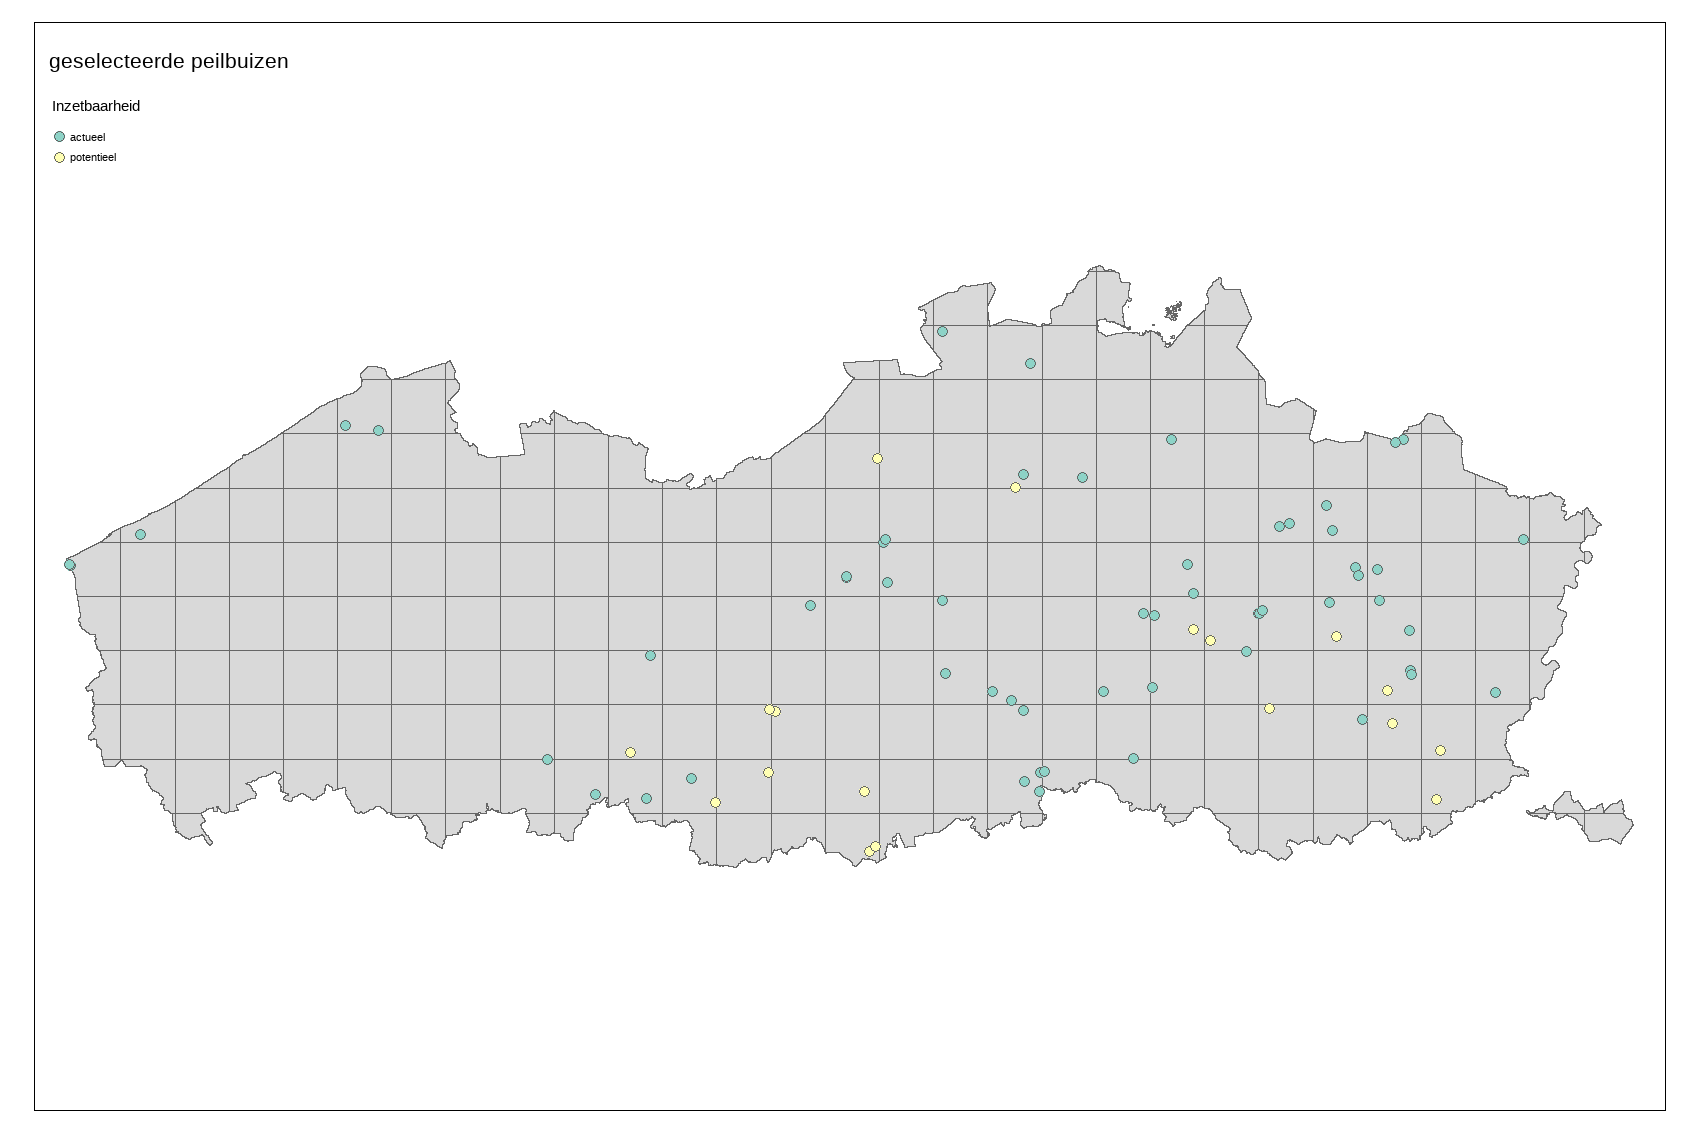
\includegraphics{droogtemeetnet_ontwerp_files/figure-latex/tubes-selected-plot-1.pdf}
\#\#\#Selecteren van potentiële geschikte habitatvlekken voor
rastercellen van categorie 1. Via een desktop-analyse zoals hieronder
beschreven wordt, kunnen slechts kandidaat habitatvlekken geselecteerd
worden. Opdat deze habitatvlek werkelijk geschikt is om er een pb te
plaatsen, vergt meestal nog nader onderzoek en meestal ook een inspectie
ter plaatse. Een kandidaat habitatvlek kan dan alsnog geweerd worden.
Alternatieve habitatvlekken liggen best in de buurt van de
oorspronkelijke kandidaat-habitatvlek, maar als je GRTS-proof werkt en
je gridcel heeft een grote oppervlakte, kan het vinden van een geschikt
alternatief leiden tot ellenlange zoektochten en veel over en weer
gerij. De hier gepresenteerde methode volgt een meer pragmatische
benadering. Elke gridcel waar het plaatsen van een pb gewenst is, wordt
eerst gecategoriseerd obv de grondwatergroepen. Elke cel van 32*32m
wordt zo in een van de vijf groepen ingedeeld. Is er voor een bepaalde
grondwatergroep een pb gewenst, dan wordt de bijhorende rastercel met
het laagste rangnummer gekozen. Deze cel ligt ingebed in een grotere
grid van bijv. 1024*1024. Hierbinnen worden de rastercellen die tot
dezelfde gw-groep behoren geselecteerd en gerangschikt volgens oplopend
rangnummer. Dit zijn bij voorkeur de alternatieve plaatsen.

Figuur \ref{fig:tubes-cat1-new} toont de verspreiding van de plaatsen
waar er bij voorkeur nog een peilbuis wordt geplaatst.

\begin{figure}
\centering
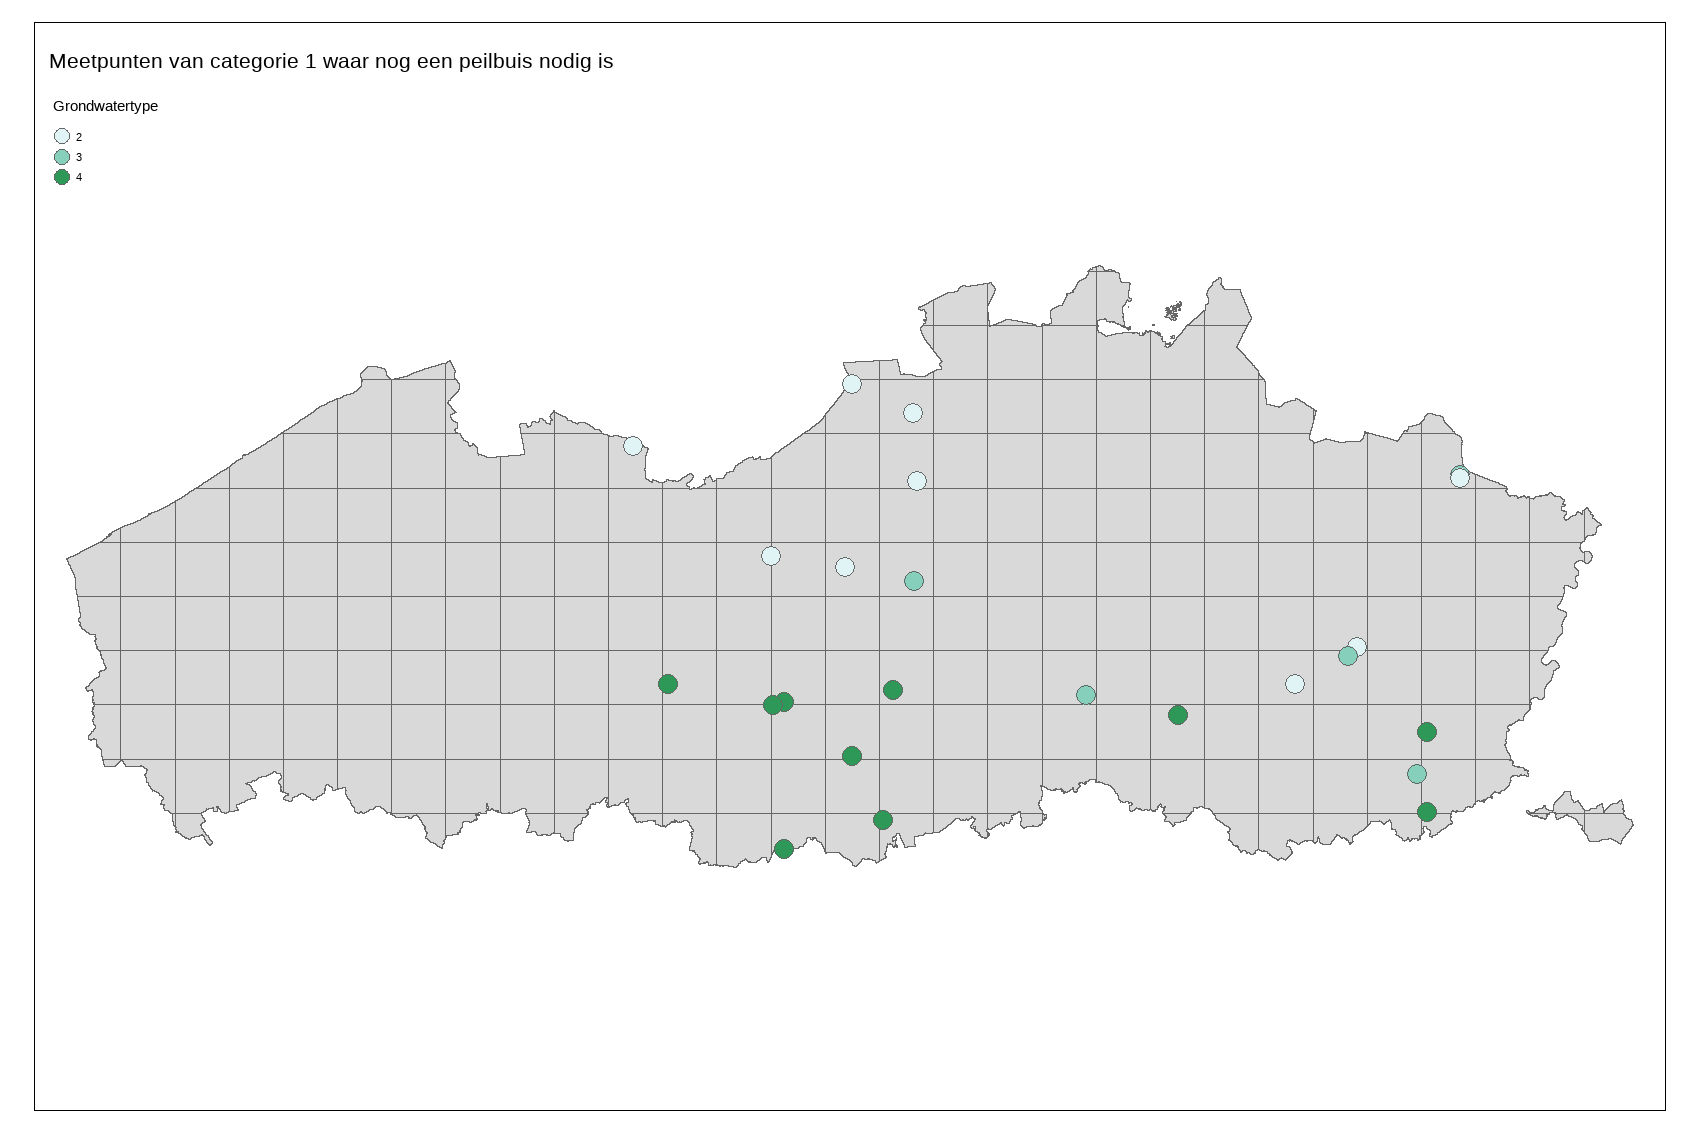
\includegraphics{droogtemeetnet_ontwerp_files/figure-latex/tubes-cat1-new-1.pdf}
\caption{\label{fig:tubes-cat1-new}Meetpunten waar nog een peilbuis nodig
is}
\end{figure}

\appendix


\chapter{Gebruikte werkomgeving}\label{gebruikte-werkomgeving}

\begin{itemize}
\tightlist
\item
  \textbf{version}: R version 3.6.1 (2019-07-05)
\item
  \textbf{os}: Windows 7 x64 SP 1
\item
  \textbf{system}: i386, mingw32
\item
  \textbf{ui}: RTerm
\item
  \textbf{language}: (EN)
\item
  \textbf{collate}: Dutch\_Belgium.1252
\item
  \textbf{ctype}: Dutch\_Belgium.1252
\item
  \textbf{tz}: Europe/Paris
\item
  \textbf{date}: 2019-11-19
\end{itemize}

\begin{longtable}[]{@{}cccc@{}}
\caption{\label{tab:sessioninfo}Loaded R packages}\tabularnewline
\toprule
\begin{minipage}[b]{0.18\columnwidth}\centering\strut
package\strut
\end{minipage} & \begin{minipage}[b]{0.19\columnwidth}\centering\strut
loadedversion\strut
\end{minipage} & \begin{minipage}[b]{0.16\columnwidth}\centering\strut
date\strut
\end{minipage} & \begin{minipage}[b]{0.36\columnwidth}\centering\strut
source\strut
\end{minipage}\tabularnewline
\midrule
\endfirsthead
\toprule
\begin{minipage}[b]{0.18\columnwidth}\centering\strut
package\strut
\end{minipage} & \begin{minipage}[b]{0.19\columnwidth}\centering\strut
loadedversion\strut
\end{minipage} & \begin{minipage}[b]{0.16\columnwidth}\centering\strut
date\strut
\end{minipage} & \begin{minipage}[b]{0.36\columnwidth}\centering\strut
source\strut
\end{minipage}\tabularnewline
\midrule
\endhead
\begin{minipage}[t]{0.18\columnwidth}\centering\strut
assertable\strut
\end{minipage} & \begin{minipage}[t]{0.19\columnwidth}\centering\strut
0.2.7\strut
\end{minipage} & \begin{minipage}[t]{0.16\columnwidth}\centering\strut
2019-09-21\strut
\end{minipage} & \begin{minipage}[t]{0.36\columnwidth}\centering\strut
CRAN (R 3.6.1)\strut
\end{minipage}\tabularnewline
\begin{minipage}[t]{0.18\columnwidth}\centering\strut
assertthat\strut
\end{minipage} & \begin{minipage}[t]{0.19\columnwidth}\centering\strut
0.2.1\strut
\end{minipage} & \begin{minipage}[t]{0.16\columnwidth}\centering\strut
2019-03-21\strut
\end{minipage} & \begin{minipage}[t]{0.36\columnwidth}\centering\strut
CRAN (R 3.6.1)\strut
\end{minipage}\tabularnewline
\begin{minipage}[t]{0.18\columnwidth}\centering\strut
backports\strut
\end{minipage} & \begin{minipage}[t]{0.19\columnwidth}\centering\strut
1.1.5\strut
\end{minipage} & \begin{minipage}[t]{0.16\columnwidth}\centering\strut
2019-10-02\strut
\end{minipage} & \begin{minipage}[t]{0.36\columnwidth}\centering\strut
CRAN (R 3.6.1)\strut
\end{minipage}\tabularnewline
\begin{minipage}[t]{0.18\columnwidth}\centering\strut
bit\strut
\end{minipage} & \begin{minipage}[t]{0.19\columnwidth}\centering\strut
1.1-14\strut
\end{minipage} & \begin{minipage}[t]{0.16\columnwidth}\centering\strut
2018-05-29\strut
\end{minipage} & \begin{minipage}[t]{0.36\columnwidth}\centering\strut
CRAN (R 3.6.0)\strut
\end{minipage}\tabularnewline
\begin{minipage}[t]{0.18\columnwidth}\centering\strut
bit64\strut
\end{minipage} & \begin{minipage}[t]{0.19\columnwidth}\centering\strut
0.9-7\strut
\end{minipage} & \begin{minipage}[t]{0.16\columnwidth}\centering\strut
2017-05-08\strut
\end{minipage} & \begin{minipage}[t]{0.36\columnwidth}\centering\strut
CRAN (R 3.6.0)\strut
\end{minipage}\tabularnewline
\begin{minipage}[t]{0.18\columnwidth}\centering\strut
blob\strut
\end{minipage} & \begin{minipage}[t]{0.19\columnwidth}\centering\strut
1.2.0\strut
\end{minipage} & \begin{minipage}[t]{0.16\columnwidth}\centering\strut
2019-07-09\strut
\end{minipage} & \begin{minipage}[t]{0.36\columnwidth}\centering\strut
CRAN (R 3.6.1)\strut
\end{minipage}\tabularnewline
\begin{minipage}[t]{0.18\columnwidth}\centering\strut
bookdown\strut
\end{minipage} & \begin{minipage}[t]{0.19\columnwidth}\centering\strut
0.14\strut
\end{minipage} & \begin{minipage}[t]{0.16\columnwidth}\centering\strut
2019-10-01\strut
\end{minipage} & \begin{minipage}[t]{0.36\columnwidth}\centering\strut
CRAN (R 3.6.1)\strut
\end{minipage}\tabularnewline
\begin{minipage}[t]{0.18\columnwidth}\centering\strut
broom\strut
\end{minipage} & \begin{minipage}[t]{0.19\columnwidth}\centering\strut
0.5.2\strut
\end{minipage} & \begin{minipage}[t]{0.16\columnwidth}\centering\strut
2019-04-07\strut
\end{minipage} & \begin{minipage}[t]{0.36\columnwidth}\centering\strut
CRAN (R 3.6.1)\strut
\end{minipage}\tabularnewline
\begin{minipage}[t]{0.18\columnwidth}\centering\strut
callr\strut
\end{minipage} & \begin{minipage}[t]{0.19\columnwidth}\centering\strut
3.3.2\strut
\end{minipage} & \begin{minipage}[t]{0.16\columnwidth}\centering\strut
2019-09-22\strut
\end{minipage} & \begin{minipage}[t]{0.36\columnwidth}\centering\strut
CRAN (R 3.6.1)\strut
\end{minipage}\tabularnewline
\begin{minipage}[t]{0.18\columnwidth}\centering\strut
cellranger\strut
\end{minipage} & \begin{minipage}[t]{0.19\columnwidth}\centering\strut
1.1.0\strut
\end{minipage} & \begin{minipage}[t]{0.16\columnwidth}\centering\strut
2016-07-27\strut
\end{minipage} & \begin{minipage}[t]{0.36\columnwidth}\centering\strut
CRAN (R 3.6.1)\strut
\end{minipage}\tabularnewline
\begin{minipage}[t]{0.18\columnwidth}\centering\strut
class\strut
\end{minipage} & \begin{minipage}[t]{0.19\columnwidth}\centering\strut
7.3-15\strut
\end{minipage} & \begin{minipage}[t]{0.16\columnwidth}\centering\strut
2019-01-01\strut
\end{minipage} & \begin{minipage}[t]{0.36\columnwidth}\centering\strut
CRAN (R 3.6.1)\strut
\end{minipage}\tabularnewline
\begin{minipage}[t]{0.18\columnwidth}\centering\strut
classInt\strut
\end{minipage} & \begin{minipage}[t]{0.19\columnwidth}\centering\strut
0.4-2\strut
\end{minipage} & \begin{minipage}[t]{0.16\columnwidth}\centering\strut
2019-10-17\strut
\end{minipage} & \begin{minipage}[t]{0.36\columnwidth}\centering\strut
CRAN (R 3.6.1)\strut
\end{minipage}\tabularnewline
\begin{minipage}[t]{0.18\columnwidth}\centering\strut
cli\strut
\end{minipage} & \begin{minipage}[t]{0.19\columnwidth}\centering\strut
1.1.0\strut
\end{minipage} & \begin{minipage}[t]{0.16\columnwidth}\centering\strut
2019-03-19\strut
\end{minipage} & \begin{minipage}[t]{0.36\columnwidth}\centering\strut
CRAN (R 3.6.1)\strut
\end{minipage}\tabularnewline
\begin{minipage}[t]{0.18\columnwidth}\centering\strut
codetools\strut
\end{minipage} & \begin{minipage}[t]{0.19\columnwidth}\centering\strut
0.2-16\strut
\end{minipage} & \begin{minipage}[t]{0.16\columnwidth}\centering\strut
2018-12-24\strut
\end{minipage} & \begin{minipage}[t]{0.36\columnwidth}\centering\strut
CRAN (R 3.6.1)\strut
\end{minipage}\tabularnewline
\begin{minipage}[t]{0.18\columnwidth}\centering\strut
colorspace\strut
\end{minipage} & \begin{minipage}[t]{0.19\columnwidth}\centering\strut
1.4-1\strut
\end{minipage} & \begin{minipage}[t]{0.16\columnwidth}\centering\strut
2019-03-18\strut
\end{minipage} & \begin{minipage}[t]{0.36\columnwidth}\centering\strut
CRAN (R 3.6.1)\strut
\end{minipage}\tabularnewline
\begin{minipage}[t]{0.18\columnwidth}\centering\strut
crayon\strut
\end{minipage} & \begin{minipage}[t]{0.19\columnwidth}\centering\strut
1.3.4\strut
\end{minipage} & \begin{minipage}[t]{0.16\columnwidth}\centering\strut
2017-09-16\strut
\end{minipage} & \begin{minipage}[t]{0.36\columnwidth}\centering\strut
CRAN (R 3.6.1)\strut
\end{minipage}\tabularnewline
\begin{minipage}[t]{0.18\columnwidth}\centering\strut
crosstalk\strut
\end{minipage} & \begin{minipage}[t]{0.19\columnwidth}\centering\strut
1.0.0\strut
\end{minipage} & \begin{minipage}[t]{0.16\columnwidth}\centering\strut
2016-12-21\strut
\end{minipage} & \begin{minipage}[t]{0.36\columnwidth}\centering\strut
CRAN (R 3.6.1)\strut
\end{minipage}\tabularnewline
\begin{minipage}[t]{0.18\columnwidth}\centering\strut
curl\strut
\end{minipage} & \begin{minipage}[t]{0.19\columnwidth}\centering\strut
4.2\strut
\end{minipage} & \begin{minipage}[t]{0.16\columnwidth}\centering\strut
2019-09-24\strut
\end{minipage} & \begin{minipage}[t]{0.36\columnwidth}\centering\strut
CRAN (R 3.6.1)\strut
\end{minipage}\tabularnewline
\begin{minipage}[t]{0.18\columnwidth}\centering\strut
data.table\strut
\end{minipage} & \begin{minipage}[t]{0.19\columnwidth}\centering\strut
1.12.6\strut
\end{minipage} & \begin{minipage}[t]{0.16\columnwidth}\centering\strut
2019-10-18\strut
\end{minipage} & \begin{minipage}[t]{0.36\columnwidth}\centering\strut
CRAN (R 3.6.1)\strut
\end{minipage}\tabularnewline
\begin{minipage}[t]{0.18\columnwidth}\centering\strut
DBI\strut
\end{minipage} & \begin{minipage}[t]{0.19\columnwidth}\centering\strut
1.0.0\strut
\end{minipage} & \begin{minipage}[t]{0.16\columnwidth}\centering\strut
2018-05-02\strut
\end{minipage} & \begin{minipage}[t]{0.36\columnwidth}\centering\strut
CRAN (R 3.6.1)\strut
\end{minipage}\tabularnewline
\begin{minipage}[t]{0.18\columnwidth}\centering\strut
dbplyr\strut
\end{minipage} & \begin{minipage}[t]{0.19\columnwidth}\centering\strut
1.4.2\strut
\end{minipage} & \begin{minipage}[t]{0.16\columnwidth}\centering\strut
2019-10-14\strut
\end{minipage} & \begin{minipage}[t]{0.36\columnwidth}\centering\strut
Github
(\href{mailto:edgararuiz/dbplyr@d8168fc}{\nolinkurl{edgararuiz/dbplyr@d8168fc}})\strut
\end{minipage}\tabularnewline
\begin{minipage}[t]{0.18\columnwidth}\centering\strut
desc\strut
\end{minipage} & \begin{minipage}[t]{0.19\columnwidth}\centering\strut
1.2.0\strut
\end{minipage} & \begin{minipage}[t]{0.16\columnwidth}\centering\strut
2018-05-01\strut
\end{minipage} & \begin{minipage}[t]{0.36\columnwidth}\centering\strut
CRAN (R 3.6.1)\strut
\end{minipage}\tabularnewline
\begin{minipage}[t]{0.18\columnwidth}\centering\strut
devtools\strut
\end{minipage} & \begin{minipage}[t]{0.19\columnwidth}\centering\strut
2.2.1\strut
\end{minipage} & \begin{minipage}[t]{0.16\columnwidth}\centering\strut
2019-09-24\strut
\end{minipage} & \begin{minipage}[t]{0.36\columnwidth}\centering\strut
CRAN (R 3.6.1)\strut
\end{minipage}\tabularnewline
\begin{minipage}[t]{0.18\columnwidth}\centering\strut
dgof\strut
\end{minipage} & \begin{minipage}[t]{0.19\columnwidth}\centering\strut
1.2\strut
\end{minipage} & \begin{minipage}[t]{0.16\columnwidth}\centering\strut
2013-10-25\strut
\end{minipage} & \begin{minipage}[t]{0.36\columnwidth}\centering\strut
CRAN (R 3.6.0)\strut
\end{minipage}\tabularnewline
\begin{minipage}[t]{0.18\columnwidth}\centering\strut
dichromat\strut
\end{minipage} & \begin{minipage}[t]{0.19\columnwidth}\centering\strut
2.0-0\strut
\end{minipage} & \begin{minipage}[t]{0.16\columnwidth}\centering\strut
2013-01-24\strut
\end{minipage} & \begin{minipage}[t]{0.36\columnwidth}\centering\strut
CRAN (R 3.6.0)\strut
\end{minipage}\tabularnewline
\begin{minipage}[t]{0.18\columnwidth}\centering\strut
digest\strut
\end{minipage} & \begin{minipage}[t]{0.19\columnwidth}\centering\strut
0.6.22\strut
\end{minipage} & \begin{minipage}[t]{0.16\columnwidth}\centering\strut
2019-10-21\strut
\end{minipage} & \begin{minipage}[t]{0.36\columnwidth}\centering\strut
CRAN (R 3.6.1)\strut
\end{minipage}\tabularnewline
\begin{minipage}[t]{0.18\columnwidth}\centering\strut
dplyr\strut
\end{minipage} & \begin{minipage}[t]{0.19\columnwidth}\centering\strut
0.8.3\strut
\end{minipage} & \begin{minipage}[t]{0.16\columnwidth}\centering\strut
2019-07-04\strut
\end{minipage} & \begin{minipage}[t]{0.36\columnwidth}\centering\strut
CRAN (R 3.6.1)\strut
\end{minipage}\tabularnewline
\begin{minipage}[t]{0.18\columnwidth}\centering\strut
e1071\strut
\end{minipage} & \begin{minipage}[t]{0.19\columnwidth}\centering\strut
1.7-2\strut
\end{minipage} & \begin{minipage}[t]{0.16\columnwidth}\centering\strut
2019-06-05\strut
\end{minipage} & \begin{minipage}[t]{0.36\columnwidth}\centering\strut
CRAN (R 3.6.1)\strut
\end{minipage}\tabularnewline
\begin{minipage}[t]{0.18\columnwidth}\centering\strut
ellipsis\strut
\end{minipage} & \begin{minipage}[t]{0.19\columnwidth}\centering\strut
0.3.0\strut
\end{minipage} & \begin{minipage}[t]{0.16\columnwidth}\centering\strut
2019-09-20\strut
\end{minipage} & \begin{minipage}[t]{0.36\columnwidth}\centering\strut
CRAN (R 3.6.1)\strut
\end{minipage}\tabularnewline
\begin{minipage}[t]{0.18\columnwidth}\centering\strut
evaluate\strut
\end{minipage} & \begin{minipage}[t]{0.19\columnwidth}\centering\strut
0.14\strut
\end{minipage} & \begin{minipage}[t]{0.16\columnwidth}\centering\strut
2019-05-28\strut
\end{minipage} & \begin{minipage}[t]{0.36\columnwidth}\centering\strut
CRAN (R 3.6.1)\strut
\end{minipage}\tabularnewline
\begin{minipage}[t]{0.18\columnwidth}\centering\strut
fastmap\strut
\end{minipage} & \begin{minipage}[t]{0.19\columnwidth}\centering\strut
1.0.1\strut
\end{minipage} & \begin{minipage}[t]{0.16\columnwidth}\centering\strut
2019-10-08\strut
\end{minipage} & \begin{minipage}[t]{0.36\columnwidth}\centering\strut
CRAN (R 3.6.1)\strut
\end{minipage}\tabularnewline
\begin{minipage}[t]{0.18\columnwidth}\centering\strut
forcats\strut
\end{minipage} & \begin{minipage}[t]{0.19\columnwidth}\centering\strut
0.4.0\strut
\end{minipage} & \begin{minipage}[t]{0.16\columnwidth}\centering\strut
2019-02-17\strut
\end{minipage} & \begin{minipage}[t]{0.36\columnwidth}\centering\strut
CRAN (R 3.6.1)\strut
\end{minipage}\tabularnewline
\begin{minipage}[t]{0.18\columnwidth}\centering\strut
foreach\strut
\end{minipage} & \begin{minipage}[t]{0.19\columnwidth}\centering\strut
1.4.7\strut
\end{minipage} & \begin{minipage}[t]{0.16\columnwidth}\centering\strut
2019-07-27\strut
\end{minipage} & \begin{minipage}[t]{0.36\columnwidth}\centering\strut
CRAN (R 3.6.1)\strut
\end{minipage}\tabularnewline
\begin{minipage}[t]{0.18\columnwidth}\centering\strut
fs\strut
\end{minipage} & \begin{minipage}[t]{0.19\columnwidth}\centering\strut
1.3.1\strut
\end{minipage} & \begin{minipage}[t]{0.16\columnwidth}\centering\strut
2019-05-06\strut
\end{minipage} & \begin{minipage}[t]{0.36\columnwidth}\centering\strut
CRAN (R 3.6.1)\strut
\end{minipage}\tabularnewline
\begin{minipage}[t]{0.18\columnwidth}\centering\strut
gdalUtils\strut
\end{minipage} & \begin{minipage}[t]{0.19\columnwidth}\centering\strut
2.0.1.14\strut
\end{minipage} & \begin{minipage}[t]{0.16\columnwidth}\centering\strut
2018-04-23\strut
\end{minipage} & \begin{minipage}[t]{0.36\columnwidth}\centering\strut
CRAN (R 3.6.1)\strut
\end{minipage}\tabularnewline
\begin{minipage}[t]{0.18\columnwidth}\centering\strut
generics\strut
\end{minipage} & \begin{minipage}[t]{0.19\columnwidth}\centering\strut
0.0.2\strut
\end{minipage} & \begin{minipage}[t]{0.16\columnwidth}\centering\strut
2018-11-29\strut
\end{minipage} & \begin{minipage}[t]{0.36\columnwidth}\centering\strut
CRAN (R 3.6.1)\strut
\end{minipage}\tabularnewline
\begin{minipage}[t]{0.18\columnwidth}\centering\strut
geoaxe\strut
\end{minipage} & \begin{minipage}[t]{0.19\columnwidth}\centering\strut
0.1.0\strut
\end{minipage} & \begin{minipage}[t]{0.16\columnwidth}\centering\strut
2016-02-19\strut
\end{minipage} & \begin{minipage}[t]{0.36\columnwidth}\centering\strut
CRAN (R 3.6.1)\strut
\end{minipage}\tabularnewline
\begin{minipage}[t]{0.18\columnwidth}\centering\strut
ggplot2\strut
\end{minipage} & \begin{minipage}[t]{0.19\columnwidth}\centering\strut
3.2.1\strut
\end{minipage} & \begin{minipage}[t]{0.16\columnwidth}\centering\strut
2019-08-10\strut
\end{minipage} & \begin{minipage}[t]{0.36\columnwidth}\centering\strut
CRAN (R 3.6.1)\strut
\end{minipage}\tabularnewline
\begin{minipage}[t]{0.18\columnwidth}\centering\strut
git2r\strut
\end{minipage} & \begin{minipage}[t]{0.19\columnwidth}\centering\strut
0.26.1\strut
\end{minipage} & \begin{minipage}[t]{0.16\columnwidth}\centering\strut
2019-06-29\strut
\end{minipage} & \begin{minipage}[t]{0.36\columnwidth}\centering\strut
CRAN (R 3.6.1)\strut
\end{minipage}\tabularnewline
\begin{minipage}[t]{0.18\columnwidth}\centering\strut
git2rdata\strut
\end{minipage} & \begin{minipage}[t]{0.19\columnwidth}\centering\strut
0.1\strut
\end{minipage} & \begin{minipage}[t]{0.16\columnwidth}\centering\strut
2019-06-17\strut
\end{minipage} & \begin{minipage}[t]{0.36\columnwidth}\centering\strut
CRAN (R 3.6.1)\strut
\end{minipage}\tabularnewline
\begin{minipage}[t]{0.18\columnwidth}\centering\strut
glue\strut
\end{minipage} & \begin{minipage}[t]{0.19\columnwidth}\centering\strut
1.3.1\strut
\end{minipage} & \begin{minipage}[t]{0.16\columnwidth}\centering\strut
2019-03-12\strut
\end{minipage} & \begin{minipage}[t]{0.36\columnwidth}\centering\strut
CRAN (R 3.6.1)\strut
\end{minipage}\tabularnewline
\begin{minipage}[t]{0.18\columnwidth}\centering\strut
googledrive\strut
\end{minipage} & \begin{minipage}[t]{0.19\columnwidth}\centering\strut
1.0.0\strut
\end{minipage} & \begin{minipage}[t]{0.16\columnwidth}\centering\strut
2019-08-19\strut
\end{minipage} & \begin{minipage}[t]{0.36\columnwidth}\centering\strut
CRAN (R 3.6.1)\strut
\end{minipage}\tabularnewline
\begin{minipage}[t]{0.18\columnwidth}\centering\strut
gtable\strut
\end{minipage} & \begin{minipage}[t]{0.19\columnwidth}\centering\strut
0.3.0\strut
\end{minipage} & \begin{minipage}[t]{0.16\columnwidth}\centering\strut
2019-03-25\strut
\end{minipage} & \begin{minipage}[t]{0.36\columnwidth}\centering\strut
CRAN (R 3.6.1)\strut
\end{minipage}\tabularnewline
\begin{minipage}[t]{0.18\columnwidth}\centering\strut
haven\strut
\end{minipage} & \begin{minipage}[t]{0.19\columnwidth}\centering\strut
2.1.1\strut
\end{minipage} & \begin{minipage}[t]{0.16\columnwidth}\centering\strut
2019-07-04\strut
\end{minipage} & \begin{minipage}[t]{0.36\columnwidth}\centering\strut
CRAN (R 3.6.1)\strut
\end{minipage}\tabularnewline
\begin{minipage}[t]{0.18\columnwidth}\centering\strut
highr\strut
\end{minipage} & \begin{minipage}[t]{0.19\columnwidth}\centering\strut
0.8\strut
\end{minipage} & \begin{minipage}[t]{0.16\columnwidth}\centering\strut
2019-03-20\strut
\end{minipage} & \begin{minipage}[t]{0.36\columnwidth}\centering\strut
CRAN (R 3.6.1)\strut
\end{minipage}\tabularnewline
\begin{minipage}[t]{0.18\columnwidth}\centering\strut
hms\strut
\end{minipage} & \begin{minipage}[t]{0.19\columnwidth}\centering\strut
0.5.1\strut
\end{minipage} & \begin{minipage}[t]{0.16\columnwidth}\centering\strut
2019-08-23\strut
\end{minipage} & \begin{minipage}[t]{0.36\columnwidth}\centering\strut
CRAN (R 3.6.1)\strut
\end{minipage}\tabularnewline
\begin{minipage}[t]{0.18\columnwidth}\centering\strut
htmltools\strut
\end{minipage} & \begin{minipage}[t]{0.19\columnwidth}\centering\strut
0.4.0\strut
\end{minipage} & \begin{minipage}[t]{0.16\columnwidth}\centering\strut
2019-10-04\strut
\end{minipage} & \begin{minipage}[t]{0.36\columnwidth}\centering\strut
CRAN (R 3.6.1)\strut
\end{minipage}\tabularnewline
\begin{minipage}[t]{0.18\columnwidth}\centering\strut
htmlwidgets\strut
\end{minipage} & \begin{minipage}[t]{0.19\columnwidth}\centering\strut
1.5.1\strut
\end{minipage} & \begin{minipage}[t]{0.16\columnwidth}\centering\strut
2019-10-08\strut
\end{minipage} & \begin{minipage}[t]{0.36\columnwidth}\centering\strut
CRAN (R 3.6.1)\strut
\end{minipage}\tabularnewline
\begin{minipage}[t]{0.18\columnwidth}\centering\strut
httpuv\strut
\end{minipage} & \begin{minipage}[t]{0.19\columnwidth}\centering\strut
1.5.2\strut
\end{minipage} & \begin{minipage}[t]{0.16\columnwidth}\centering\strut
2019-09-11\strut
\end{minipage} & \begin{minipage}[t]{0.36\columnwidth}\centering\strut
CRAN (R 3.6.1)\strut
\end{minipage}\tabularnewline
\begin{minipage}[t]{0.18\columnwidth}\centering\strut
httr\strut
\end{minipage} & \begin{minipage}[t]{0.19\columnwidth}\centering\strut
1.4.1\strut
\end{minipage} & \begin{minipage}[t]{0.16\columnwidth}\centering\strut
2019-08-05\strut
\end{minipage} & \begin{minipage}[t]{0.36\columnwidth}\centering\strut
CRAN (R 3.6.1)\strut
\end{minipage}\tabularnewline
\begin{minipage}[t]{0.18\columnwidth}\centering\strut
inborutils\strut
\end{minipage} & \begin{minipage}[t]{0.19\columnwidth}\centering\strut
0.1.0.9062\strut
\end{minipage} & \begin{minipage}[t]{0.16\columnwidth}\centering\strut
2019-09-18\strut
\end{minipage} & \begin{minipage}[t]{0.36\columnwidth}\centering\strut
Github
(\href{mailto:inbo/inborutils@4c0dc7a}{\nolinkurl{inbo/inborutils@4c0dc7a}})\strut
\end{minipage}\tabularnewline
\begin{minipage}[t]{0.18\columnwidth}\centering\strut
iterators\strut
\end{minipage} & \begin{minipage}[t]{0.19\columnwidth}\centering\strut
1.0.12\strut
\end{minipage} & \begin{minipage}[t]{0.16\columnwidth}\centering\strut
2019-07-26\strut
\end{minipage} & \begin{minipage}[t]{0.36\columnwidth}\centering\strut
CRAN (R 3.6.1)\strut
\end{minipage}\tabularnewline
\begin{minipage}[t]{0.18\columnwidth}\centering\strut
janitor\strut
\end{minipage} & \begin{minipage}[t]{0.19\columnwidth}\centering\strut
1.2.0\strut
\end{minipage} & \begin{minipage}[t]{0.16\columnwidth}\centering\strut
2019-04-21\strut
\end{minipage} & \begin{minipage}[t]{0.36\columnwidth}\centering\strut
CRAN (R 3.6.1)\strut
\end{minipage}\tabularnewline
\begin{minipage}[t]{0.18\columnwidth}\centering\strut
jsonlite\strut
\end{minipage} & \begin{minipage}[t]{0.19\columnwidth}\centering\strut
1.6\strut
\end{minipage} & \begin{minipage}[t]{0.16\columnwidth}\centering\strut
2018-12-07\strut
\end{minipage} & \begin{minipage}[t]{0.36\columnwidth}\centering\strut
CRAN (R 3.6.1)\strut
\end{minipage}\tabularnewline
\begin{minipage}[t]{0.18\columnwidth}\centering\strut
kableExtra\strut
\end{minipage} & \begin{minipage}[t]{0.19\columnwidth}\centering\strut
1.1.0\strut
\end{minipage} & \begin{minipage}[t]{0.16\columnwidth}\centering\strut
2019-03-16\strut
\end{minipage} & \begin{minipage}[t]{0.36\columnwidth}\centering\strut
CRAN (R 3.6.1)\strut
\end{minipage}\tabularnewline
\begin{minipage}[t]{0.18\columnwidth}\centering\strut
KernSmooth\strut
\end{minipage} & \begin{minipage}[t]{0.19\columnwidth}\centering\strut
2.23-16\strut
\end{minipage} & \begin{minipage}[t]{0.16\columnwidth}\centering\strut
2019-10-15\strut
\end{minipage} & \begin{minipage}[t]{0.36\columnwidth}\centering\strut
CRAN (R 3.6.1)\strut
\end{minipage}\tabularnewline
\begin{minipage}[t]{0.18\columnwidth}\centering\strut
knitr\strut
\end{minipage} & \begin{minipage}[t]{0.19\columnwidth}\centering\strut
1.25\strut
\end{minipage} & \begin{minipage}[t]{0.16\columnwidth}\centering\strut
2019-09-18\strut
\end{minipage} & \begin{minipage}[t]{0.36\columnwidth}\centering\strut
CRAN (R 3.6.1)\strut
\end{minipage}\tabularnewline
\begin{minipage}[t]{0.18\columnwidth}\centering\strut
KSgeneral\strut
\end{minipage} & \begin{minipage}[t]{0.19\columnwidth}\centering\strut
0.1.1\strut
\end{minipage} & \begin{minipage}[t]{0.16\columnwidth}\centering\strut
2018-05-14\strut
\end{minipage} & \begin{minipage}[t]{0.36\columnwidth}\centering\strut
CRAN (R 3.6.1)\strut
\end{minipage}\tabularnewline
\begin{minipage}[t]{0.18\columnwidth}\centering\strut
later\strut
\end{minipage} & \begin{minipage}[t]{0.19\columnwidth}\centering\strut
1.0.0\strut
\end{minipage} & \begin{minipage}[t]{0.16\columnwidth}\centering\strut
2019-10-04\strut
\end{minipage} & \begin{minipage}[t]{0.36\columnwidth}\centering\strut
CRAN (R 3.6.1)\strut
\end{minipage}\tabularnewline
\begin{minipage}[t]{0.18\columnwidth}\centering\strut
lattice\strut
\end{minipage} & \begin{minipage}[t]{0.19\columnwidth}\centering\strut
0.20-38\strut
\end{minipage} & \begin{minipage}[t]{0.16\columnwidth}\centering\strut
2018-11-04\strut
\end{minipage} & \begin{minipage}[t]{0.36\columnwidth}\centering\strut
CRAN (R 3.6.1)\strut
\end{minipage}\tabularnewline
\begin{minipage}[t]{0.18\columnwidth}\centering\strut
lazyeval\strut
\end{minipage} & \begin{minipage}[t]{0.19\columnwidth}\centering\strut
0.2.2\strut
\end{minipage} & \begin{minipage}[t]{0.16\columnwidth}\centering\strut
2019-03-15\strut
\end{minipage} & \begin{minipage}[t]{0.36\columnwidth}\centering\strut
CRAN (R 3.6.1)\strut
\end{minipage}\tabularnewline
\begin{minipage}[t]{0.18\columnwidth}\centering\strut
leaflet\strut
\end{minipage} & \begin{minipage}[t]{0.19\columnwidth}\centering\strut
2.0.2\strut
\end{minipage} & \begin{minipage}[t]{0.16\columnwidth}\centering\strut
2018-08-27\strut
\end{minipage} & \begin{minipage}[t]{0.36\columnwidth}\centering\strut
CRAN (R 3.5.3)\strut
\end{minipage}\tabularnewline
\begin{minipage}[t]{0.18\columnwidth}\centering\strut
leafsync\strut
\end{minipage} & \begin{minipage}[t]{0.19\columnwidth}\centering\strut
0.1.0\strut
\end{minipage} & \begin{minipage}[t]{0.16\columnwidth}\centering\strut
2019-03-05\strut
\end{minipage} & \begin{minipage}[t]{0.36\columnwidth}\centering\strut
CRAN (R 3.6.1)\strut
\end{minipage}\tabularnewline
\begin{minipage}[t]{0.18\columnwidth}\centering\strut
lifecycle\strut
\end{minipage} & \begin{minipage}[t]{0.19\columnwidth}\centering\strut
0.1.0\strut
\end{minipage} & \begin{minipage}[t]{0.16\columnwidth}\centering\strut
2019-08-01\strut
\end{minipage} & \begin{minipage}[t]{0.36\columnwidth}\centering\strut
CRAN (R 3.6.1)\strut
\end{minipage}\tabularnewline
\begin{minipage}[t]{0.18\columnwidth}\centering\strut
lubridate\strut
\end{minipage} & \begin{minipage}[t]{0.19\columnwidth}\centering\strut
1.7.4\strut
\end{minipage} & \begin{minipage}[t]{0.16\columnwidth}\centering\strut
2018-04-11\strut
\end{minipage} & \begin{minipage}[t]{0.36\columnwidth}\centering\strut
CRAN (R 3.6.1)\strut
\end{minipage}\tabularnewline
\begin{minipage}[t]{0.18\columnwidth}\centering\strut
lwgeom\strut
\end{minipage} & \begin{minipage}[t]{0.19\columnwidth}\centering\strut
0.1-7\strut
\end{minipage} & \begin{minipage}[t]{0.16\columnwidth}\centering\strut
2019-05-06\strut
\end{minipage} & \begin{minipage}[t]{0.36\columnwidth}\centering\strut
CRAN (R 3.6.1)\strut
\end{minipage}\tabularnewline
\begin{minipage}[t]{0.18\columnwidth}\centering\strut
magrittr\strut
\end{minipage} & \begin{minipage}[t]{0.19\columnwidth}\centering\strut
1.5\strut
\end{minipage} & \begin{minipage}[t]{0.16\columnwidth}\centering\strut
2014-11-22\strut
\end{minipage} & \begin{minipage}[t]{0.36\columnwidth}\centering\strut
CRAN (R 3.6.1)\strut
\end{minipage}\tabularnewline
\begin{minipage}[t]{0.18\columnwidth}\centering\strut
MASS\strut
\end{minipage} & \begin{minipage}[t]{0.19\columnwidth}\centering\strut
7.3-51.4\strut
\end{minipage} & \begin{minipage}[t]{0.16\columnwidth}\centering\strut
2019-03-31\strut
\end{minipage} & \begin{minipage}[t]{0.36\columnwidth}\centering\strut
CRAN (R 3.6.1)\strut
\end{minipage}\tabularnewline
\begin{minipage}[t]{0.18\columnwidth}\centering\strut
memoise\strut
\end{minipage} & \begin{minipage}[t]{0.19\columnwidth}\centering\strut
1.1.0\strut
\end{minipage} & \begin{minipage}[t]{0.16\columnwidth}\centering\strut
2017-04-21\strut
\end{minipage} & \begin{minipage}[t]{0.36\columnwidth}\centering\strut
CRAN (R 3.6.1)\strut
\end{minipage}\tabularnewline
\begin{minipage}[t]{0.18\columnwidth}\centering\strut
mime\strut
\end{minipage} & \begin{minipage}[t]{0.19\columnwidth}\centering\strut
0.7\strut
\end{minipage} & \begin{minipage}[t]{0.16\columnwidth}\centering\strut
2019-06-11\strut
\end{minipage} & \begin{minipage}[t]{0.36\columnwidth}\centering\strut
CRAN (R 3.6.0)\strut
\end{minipage}\tabularnewline
\begin{minipage}[t]{0.18\columnwidth}\centering\strut
modelr\strut
\end{minipage} & \begin{minipage}[t]{0.19\columnwidth}\centering\strut
0.1.5\strut
\end{minipage} & \begin{minipage}[t]{0.16\columnwidth}\centering\strut
2019-08-08\strut
\end{minipage} & \begin{minipage}[t]{0.36\columnwidth}\centering\strut
CRAN (R 3.6.1)\strut
\end{minipage}\tabularnewline
\begin{minipage}[t]{0.18\columnwidth}\centering\strut
munsell\strut
\end{minipage} & \begin{minipage}[t]{0.19\columnwidth}\centering\strut
0.5.0\strut
\end{minipage} & \begin{minipage}[t]{0.16\columnwidth}\centering\strut
2018-06-12\strut
\end{minipage} & \begin{minipage}[t]{0.36\columnwidth}\centering\strut
CRAN (R 3.6.1)\strut
\end{minipage}\tabularnewline
\begin{minipage}[t]{0.18\columnwidth}\centering\strut
n2khab\strut
\end{minipage} & \begin{minipage}[t]{0.19\columnwidth}\centering\strut
0.0.3.9037\strut
\end{minipage} & \begin{minipage}[t]{0.16\columnwidth}\centering\strut
2019-11-07\strut
\end{minipage} & \begin{minipage}[t]{0.36\columnwidth}\centering\strut
Github
(\href{mailto:inbo/n2khab@1aa3f85}{\nolinkurl{inbo/n2khab@1aa3f85}})\strut
\end{minipage}\tabularnewline
\begin{minipage}[t]{0.18\columnwidth}\centering\strut
nlme\strut
\end{minipage} & \begin{minipage}[t]{0.19\columnwidth}\centering\strut
3.1-141\strut
\end{minipage} & \begin{minipage}[t]{0.16\columnwidth}\centering\strut
2019-08-01\strut
\end{minipage} & \begin{minipage}[t]{0.36\columnwidth}\centering\strut
CRAN (R 3.6.1)\strut
\end{minipage}\tabularnewline
\begin{minipage}[t]{0.18\columnwidth}\centering\strut
oai\strut
\end{minipage} & \begin{minipage}[t]{0.19\columnwidth}\centering\strut
0.3.0\strut
\end{minipage} & \begin{minipage}[t]{0.16\columnwidth}\centering\strut
2019-09-07\strut
\end{minipage} & \begin{minipage}[t]{0.36\columnwidth}\centering\strut
CRAN (R 3.6.1)\strut
\end{minipage}\tabularnewline
\begin{minipage}[t]{0.18\columnwidth}\centering\strut
odbc\strut
\end{minipage} & \begin{minipage}[t]{0.19\columnwidth}\centering\strut
1.1.6\strut
\end{minipage} & \begin{minipage}[t]{0.16\columnwidth}\centering\strut
2018-06-09\strut
\end{minipage} & \begin{minipage}[t]{0.36\columnwidth}\centering\strut
CRAN (R 3.6.1)\strut
\end{minipage}\tabularnewline
\begin{minipage}[t]{0.18\columnwidth}\centering\strut
pillar\strut
\end{minipage} & \begin{minipage}[t]{0.19\columnwidth}\centering\strut
1.4.2\strut
\end{minipage} & \begin{minipage}[t]{0.16\columnwidth}\centering\strut
2019-06-29\strut
\end{minipage} & \begin{minipage}[t]{0.36\columnwidth}\centering\strut
CRAN (R 3.6.1)\strut
\end{minipage}\tabularnewline
\begin{minipage}[t]{0.18\columnwidth}\centering\strut
pkgbuild\strut
\end{minipage} & \begin{minipage}[t]{0.19\columnwidth}\centering\strut
1.0.6\strut
\end{minipage} & \begin{minipage}[t]{0.16\columnwidth}\centering\strut
2019-10-09\strut
\end{minipage} & \begin{minipage}[t]{0.36\columnwidth}\centering\strut
CRAN (R 3.6.1)\strut
\end{minipage}\tabularnewline
\begin{minipage}[t]{0.18\columnwidth}\centering\strut
pkgconfig\strut
\end{minipage} & \begin{minipage}[t]{0.19\columnwidth}\centering\strut
2.0.3\strut
\end{minipage} & \begin{minipage}[t]{0.16\columnwidth}\centering\strut
2019-09-22\strut
\end{minipage} & \begin{minipage}[t]{0.36\columnwidth}\centering\strut
CRAN (R 3.6.1)\strut
\end{minipage}\tabularnewline
\begin{minipage}[t]{0.18\columnwidth}\centering\strut
pkgload\strut
\end{minipage} & \begin{minipage}[t]{0.19\columnwidth}\centering\strut
1.0.2\strut
\end{minipage} & \begin{minipage}[t]{0.16\columnwidth}\centering\strut
2018-10-29\strut
\end{minipage} & \begin{minipage}[t]{0.36\columnwidth}\centering\strut
CRAN (R 3.6.1)\strut
\end{minipage}\tabularnewline
\begin{minipage}[t]{0.18\columnwidth}\centering\strut
plyr\strut
\end{minipage} & \begin{minipage}[t]{0.19\columnwidth}\centering\strut
1.8.4\strut
\end{minipage} & \begin{minipage}[t]{0.16\columnwidth}\centering\strut
2016-06-08\strut
\end{minipage} & \begin{minipage}[t]{0.36\columnwidth}\centering\strut
CRAN (R 3.6.1)\strut
\end{minipage}\tabularnewline
\begin{minipage}[t]{0.18\columnwidth}\centering\strut
png\strut
\end{minipage} & \begin{minipage}[t]{0.19\columnwidth}\centering\strut
0.1-7\strut
\end{minipage} & \begin{minipage}[t]{0.16\columnwidth}\centering\strut
2013-12-03\strut
\end{minipage} & \begin{minipage}[t]{0.36\columnwidth}\centering\strut
CRAN (R 3.6.0)\strut
\end{minipage}\tabularnewline
\begin{minipage}[t]{0.18\columnwidth}\centering\strut
prettyunits\strut
\end{minipage} & \begin{minipage}[t]{0.19\columnwidth}\centering\strut
1.0.2\strut
\end{minipage} & \begin{minipage}[t]{0.16\columnwidth}\centering\strut
2015-07-13\strut
\end{minipage} & \begin{minipage}[t]{0.36\columnwidth}\centering\strut
CRAN (R 3.6.1)\strut
\end{minipage}\tabularnewline
\begin{minipage}[t]{0.18\columnwidth}\centering\strut
processx\strut
\end{minipage} & \begin{minipage}[t]{0.19\columnwidth}\centering\strut
3.4.1\strut
\end{minipage} & \begin{minipage}[t]{0.16\columnwidth}\centering\strut
2019-07-18\strut
\end{minipage} & \begin{minipage}[t]{0.36\columnwidth}\centering\strut
CRAN (R 3.6.1)\strut
\end{minipage}\tabularnewline
\begin{minipage}[t]{0.18\columnwidth}\centering\strut
promises\strut
\end{minipage} & \begin{minipage}[t]{0.19\columnwidth}\centering\strut
1.1.0\strut
\end{minipage} & \begin{minipage}[t]{0.16\columnwidth}\centering\strut
2019-10-04\strut
\end{minipage} & \begin{minipage}[t]{0.36\columnwidth}\centering\strut
CRAN (R 3.6.1)\strut
\end{minipage}\tabularnewline
\begin{minipage}[t]{0.18\columnwidth}\centering\strut
ps\strut
\end{minipage} & \begin{minipage}[t]{0.19\columnwidth}\centering\strut
1.3.0\strut
\end{minipage} & \begin{minipage}[t]{0.16\columnwidth}\centering\strut
2018-12-21\strut
\end{minipage} & \begin{minipage}[t]{0.36\columnwidth}\centering\strut
CRAN (R 3.6.1)\strut
\end{minipage}\tabularnewline
\begin{minipage}[t]{0.18\columnwidth}\centering\strut
purrr\strut
\end{minipage} & \begin{minipage}[t]{0.19\columnwidth}\centering\strut
0.3.3\strut
\end{minipage} & \begin{minipage}[t]{0.16\columnwidth}\centering\strut
2019-10-18\strut
\end{minipage} & \begin{minipage}[t]{0.36\columnwidth}\centering\strut
CRAN (R 3.6.1)\strut
\end{minipage}\tabularnewline
\begin{minipage}[t]{0.18\columnwidth}\centering\strut
R.methodsS3\strut
\end{minipage} & \begin{minipage}[t]{0.19\columnwidth}\centering\strut
1.7.1\strut
\end{minipage} & \begin{minipage}[t]{0.16\columnwidth}\centering\strut
2016-02-16\strut
\end{minipage} & \begin{minipage}[t]{0.36\columnwidth}\centering\strut
CRAN (R 3.6.0)\strut
\end{minipage}\tabularnewline
\begin{minipage}[t]{0.18\columnwidth}\centering\strut
R.oo\strut
\end{minipage} & \begin{minipage}[t]{0.19\columnwidth}\centering\strut
1.22.0\strut
\end{minipage} & \begin{minipage}[t]{0.16\columnwidth}\centering\strut
2018-04-22\strut
\end{minipage} & \begin{minipage}[t]{0.36\columnwidth}\centering\strut
CRAN (R 3.6.0)\strut
\end{minipage}\tabularnewline
\begin{minipage}[t]{0.18\columnwidth}\centering\strut
R.utils\strut
\end{minipage} & \begin{minipage}[t]{0.19\columnwidth}\centering\strut
2.9.0\strut
\end{minipage} & \begin{minipage}[t]{0.16\columnwidth}\centering\strut
2019-06-13\strut
\end{minipage} & \begin{minipage}[t]{0.36\columnwidth}\centering\strut
CRAN (R 3.6.1)\strut
\end{minipage}\tabularnewline
\begin{minipage}[t]{0.18\columnwidth}\centering\strut
R6\strut
\end{minipage} & \begin{minipage}[t]{0.19\columnwidth}\centering\strut
2.4.0\strut
\end{minipage} & \begin{minipage}[t]{0.16\columnwidth}\centering\strut
2019-02-14\strut
\end{minipage} & \begin{minipage}[t]{0.36\columnwidth}\centering\strut
CRAN (R 3.6.1)\strut
\end{minipage}\tabularnewline
\begin{minipage}[t]{0.18\columnwidth}\centering\strut
raster\strut
\end{minipage} & \begin{minipage}[t]{0.19\columnwidth}\centering\strut
3.0-7\strut
\end{minipage} & \begin{minipage}[t]{0.16\columnwidth}\centering\strut
2019-09-24\strut
\end{minipage} & \begin{minipage}[t]{0.36\columnwidth}\centering\strut
CRAN (R 3.6.1)\strut
\end{minipage}\tabularnewline
\begin{minipage}[t]{0.18\columnwidth}\centering\strut
RColorBrewer\strut
\end{minipage} & \begin{minipage}[t]{0.19\columnwidth}\centering\strut
1.1-2\strut
\end{minipage} & \begin{minipage}[t]{0.16\columnwidth}\centering\strut
2014-12-07\strut
\end{minipage} & \begin{minipage}[t]{0.36\columnwidth}\centering\strut
CRAN (R 3.6.0)\strut
\end{minipage}\tabularnewline
\begin{minipage}[t]{0.18\columnwidth}\centering\strut
Rcpp\strut
\end{minipage} & \begin{minipage}[t]{0.19\columnwidth}\centering\strut
1.0.2\strut
\end{minipage} & \begin{minipage}[t]{0.16\columnwidth}\centering\strut
2019-07-25\strut
\end{minipage} & \begin{minipage}[t]{0.36\columnwidth}\centering\strut
CRAN (R 3.6.1)\strut
\end{minipage}\tabularnewline
\begin{minipage}[t]{0.18\columnwidth}\centering\strut
readr\strut
\end{minipage} & \begin{minipage}[t]{0.19\columnwidth}\centering\strut
1.3.1\strut
\end{minipage} & \begin{minipage}[t]{0.16\columnwidth}\centering\strut
2018-12-21\strut
\end{minipage} & \begin{minipage}[t]{0.36\columnwidth}\centering\strut
CRAN (R 3.6.1)\strut
\end{minipage}\tabularnewline
\begin{minipage}[t]{0.18\columnwidth}\centering\strut
readxl\strut
\end{minipage} & \begin{minipage}[t]{0.19\columnwidth}\centering\strut
1.3.1\strut
\end{minipage} & \begin{minipage}[t]{0.16\columnwidth}\centering\strut
2019-03-13\strut
\end{minipage} & \begin{minipage}[t]{0.36\columnwidth}\centering\strut
CRAN (R 3.6.1)\strut
\end{minipage}\tabularnewline
\begin{minipage}[t]{0.18\columnwidth}\centering\strut
remotes\strut
\end{minipage} & \begin{minipage}[t]{0.19\columnwidth}\centering\strut
2.1.0\strut
\end{minipage} & \begin{minipage}[t]{0.16\columnwidth}\centering\strut
2019-06-24\strut
\end{minipage} & \begin{minipage}[t]{0.36\columnwidth}\centering\strut
CRAN (R 3.6.1)\strut
\end{minipage}\tabularnewline
\begin{minipage}[t]{0.18\columnwidth}\centering\strut
rgbif\strut
\end{minipage} & \begin{minipage}[t]{0.19\columnwidth}\centering\strut
1.3.0\strut
\end{minipage} & \begin{minipage}[t]{0.16\columnwidth}\centering\strut
2019-05-08\strut
\end{minipage} & \begin{minipage}[t]{0.36\columnwidth}\centering\strut
CRAN (R 3.6.1)\strut
\end{minipage}\tabularnewline
\begin{minipage}[t]{0.18\columnwidth}\centering\strut
rgdal\strut
\end{minipage} & \begin{minipage}[t]{0.19\columnwidth}\centering\strut
1.4-6\strut
\end{minipage} & \begin{minipage}[t]{0.16\columnwidth}\centering\strut
2019-10-01\strut
\end{minipage} & \begin{minipage}[t]{0.36\columnwidth}\centering\strut
CRAN (R 3.6.1)\strut
\end{minipage}\tabularnewline
\begin{minipage}[t]{0.18\columnwidth}\centering\strut
rgeos\strut
\end{minipage} & \begin{minipage}[t]{0.19\columnwidth}\centering\strut
0.5-2\strut
\end{minipage} & \begin{minipage}[t]{0.16\columnwidth}\centering\strut
2019-10-03\strut
\end{minipage} & \begin{minipage}[t]{0.36\columnwidth}\centering\strut
CRAN (R 3.6.1)\strut
\end{minipage}\tabularnewline
\begin{minipage}[t]{0.18\columnwidth}\centering\strut
rlang\strut
\end{minipage} & \begin{minipage}[t]{0.19\columnwidth}\centering\strut
0.4.1\strut
\end{minipage} & \begin{minipage}[t]{0.16\columnwidth}\centering\strut
2019-10-24\strut
\end{minipage} & \begin{minipage}[t]{0.36\columnwidth}\centering\strut
CRAN (R 3.6.1)\strut
\end{minipage}\tabularnewline
\begin{minipage}[t]{0.18\columnwidth}\centering\strut
rmarkdown\strut
\end{minipage} & \begin{minipage}[t]{0.19\columnwidth}\centering\strut
1.16\strut
\end{minipage} & \begin{minipage}[t]{0.16\columnwidth}\centering\strut
2019-10-01\strut
\end{minipage} & \begin{minipage}[t]{0.36\columnwidth}\centering\strut
CRAN (R 3.6.1)\strut
\end{minipage}\tabularnewline
\begin{minipage}[t]{0.18\columnwidth}\centering\strut
rprojroot\strut
\end{minipage} & \begin{minipage}[t]{0.19\columnwidth}\centering\strut
1.3-2\strut
\end{minipage} & \begin{minipage}[t]{0.16\columnwidth}\centering\strut
2018-01-03\strut
\end{minipage} & \begin{minipage}[t]{0.36\columnwidth}\centering\strut
CRAN (R 3.6.1)\strut
\end{minipage}\tabularnewline
\begin{minipage}[t]{0.18\columnwidth}\centering\strut
RSQLite\strut
\end{minipage} & \begin{minipage}[t]{0.19\columnwidth}\centering\strut
2.1.2\strut
\end{minipage} & \begin{minipage}[t]{0.16\columnwidth}\centering\strut
2019-07-24\strut
\end{minipage} & \begin{minipage}[t]{0.36\columnwidth}\centering\strut
CRAN (R 3.6.1)\strut
\end{minipage}\tabularnewline
\begin{minipage}[t]{0.18\columnwidth}\centering\strut
rstudioapi\strut
\end{minipage} & \begin{minipage}[t]{0.19\columnwidth}\centering\strut
0.10.0-9001\strut
\end{minipage} & \begin{minipage}[t]{0.16\columnwidth}\centering\strut
2019-09-18\strut
\end{minipage} & \begin{minipage}[t]{0.36\columnwidth}\centering\strut
Github
(\href{mailto:rstudio/rstudioapi@af40e20}{\nolinkurl{rstudio/rstudioapi@af40e20}})\strut
\end{minipage}\tabularnewline
\begin{minipage}[t]{0.18\columnwidth}\centering\strut
rvest\strut
\end{minipage} & \begin{minipage}[t]{0.19\columnwidth}\centering\strut
0.3.4\strut
\end{minipage} & \begin{minipage}[t]{0.16\columnwidth}\centering\strut
2019-05-15\strut
\end{minipage} & \begin{minipage}[t]{0.36\columnwidth}\centering\strut
CRAN (R 3.6.1)\strut
\end{minipage}\tabularnewline
\begin{minipage}[t]{0.18\columnwidth}\centering\strut
scales\strut
\end{minipage} & \begin{minipage}[t]{0.19\columnwidth}\centering\strut
1.0.0\strut
\end{minipage} & \begin{minipage}[t]{0.16\columnwidth}\centering\strut
2018-08-09\strut
\end{minipage} & \begin{minipage}[t]{0.36\columnwidth}\centering\strut
CRAN (R 3.6.1)\strut
\end{minipage}\tabularnewline
\begin{minipage}[t]{0.18\columnwidth}\centering\strut
sessioninfo\strut
\end{minipage} & \begin{minipage}[t]{0.19\columnwidth}\centering\strut
1.1.1\strut
\end{minipage} & \begin{minipage}[t]{0.16\columnwidth}\centering\strut
2018-11-05\strut
\end{minipage} & \begin{minipage}[t]{0.36\columnwidth}\centering\strut
CRAN (R 3.6.1)\strut
\end{minipage}\tabularnewline
\begin{minipage}[t]{0.18\columnwidth}\centering\strut
sf\strut
\end{minipage} & \begin{minipage}[t]{0.19\columnwidth}\centering\strut
0.8-0\strut
\end{minipage} & \begin{minipage}[t]{0.16\columnwidth}\centering\strut
2019-09-17\strut
\end{minipage} & \begin{minipage}[t]{0.36\columnwidth}\centering\strut
CRAN (R 3.6.1)\strut
\end{minipage}\tabularnewline
\begin{minipage}[t]{0.18\columnwidth}\centering\strut
shiny\strut
\end{minipage} & \begin{minipage}[t]{0.19\columnwidth}\centering\strut
1.4.0\strut
\end{minipage} & \begin{minipage}[t]{0.16\columnwidth}\centering\strut
2019-10-10\strut
\end{minipage} & \begin{minipage}[t]{0.36\columnwidth}\centering\strut
CRAN (R 3.6.1)\strut
\end{minipage}\tabularnewline
\begin{minipage}[t]{0.18\columnwidth}\centering\strut
snakecase\strut
\end{minipage} & \begin{minipage}[t]{0.19\columnwidth}\centering\strut
0.11.0\strut
\end{minipage} & \begin{minipage}[t]{0.16\columnwidth}\centering\strut
2019-05-25\strut
\end{minipage} & \begin{minipage}[t]{0.36\columnwidth}\centering\strut
CRAN (R 3.6.1)\strut
\end{minipage}\tabularnewline
\begin{minipage}[t]{0.18\columnwidth}\centering\strut
sp\strut
\end{minipage} & \begin{minipage}[t]{0.19\columnwidth}\centering\strut
1.3-1\strut
\end{minipage} & \begin{minipage}[t]{0.16\columnwidth}\centering\strut
2018-06-05\strut
\end{minipage} & \begin{minipage}[t]{0.36\columnwidth}\centering\strut
CRAN (R 3.6.1)\strut
\end{minipage}\tabularnewline
\begin{minipage}[t]{0.18\columnwidth}\centering\strut
stringi\strut
\end{minipage} & \begin{minipage}[t]{0.19\columnwidth}\centering\strut
1.4.3\strut
\end{minipage} & \begin{minipage}[t]{0.16\columnwidth}\centering\strut
2019-03-12\strut
\end{minipage} & \begin{minipage}[t]{0.36\columnwidth}\centering\strut
CRAN (R 3.6.0)\strut
\end{minipage}\tabularnewline
\begin{minipage}[t]{0.18\columnwidth}\centering\strut
stringr\strut
\end{minipage} & \begin{minipage}[t]{0.19\columnwidth}\centering\strut
1.4.0\strut
\end{minipage} & \begin{minipage}[t]{0.16\columnwidth}\centering\strut
2019-02-10\strut
\end{minipage} & \begin{minipage}[t]{0.36\columnwidth}\centering\strut
CRAN (R 3.6.1)\strut
\end{minipage}\tabularnewline
\begin{minipage}[t]{0.18\columnwidth}\centering\strut
testthat\strut
\end{minipage} & \begin{minipage}[t]{0.19\columnwidth}\centering\strut
2.2.1\strut
\end{minipage} & \begin{minipage}[t]{0.16\columnwidth}\centering\strut
2019-07-25\strut
\end{minipage} & \begin{minipage}[t]{0.36\columnwidth}\centering\strut
CRAN (R 3.6.1)\strut
\end{minipage}\tabularnewline
\begin{minipage}[t]{0.18\columnwidth}\centering\strut
tibble\strut
\end{minipage} & \begin{minipage}[t]{0.19\columnwidth}\centering\strut
2.1.3\strut
\end{minipage} & \begin{minipage}[t]{0.16\columnwidth}\centering\strut
2019-06-06\strut
\end{minipage} & \begin{minipage}[t]{0.36\columnwidth}\centering\strut
CRAN (R 3.6.1)\strut
\end{minipage}\tabularnewline
\begin{minipage}[t]{0.18\columnwidth}\centering\strut
tidyr\strut
\end{minipage} & \begin{minipage}[t]{0.19\columnwidth}\centering\strut
1.0.0\strut
\end{minipage} & \begin{minipage}[t]{0.16\columnwidth}\centering\strut
2019-09-11\strut
\end{minipage} & \begin{minipage}[t]{0.36\columnwidth}\centering\strut
CRAN (R 3.6.1)\strut
\end{minipage}\tabularnewline
\begin{minipage}[t]{0.18\columnwidth}\centering\strut
tidyselect\strut
\end{minipage} & \begin{minipage}[t]{0.19\columnwidth}\centering\strut
0.2.5\strut
\end{minipage} & \begin{minipage}[t]{0.16\columnwidth}\centering\strut
2018-10-11\strut
\end{minipage} & \begin{minipage}[t]{0.36\columnwidth}\centering\strut
CRAN (R 3.6.1)\strut
\end{minipage}\tabularnewline
\begin{minipage}[t]{0.18\columnwidth}\centering\strut
tidyverse\strut
\end{minipage} & \begin{minipage}[t]{0.19\columnwidth}\centering\strut
1.2.1\strut
\end{minipage} & \begin{minipage}[t]{0.16\columnwidth}\centering\strut
2017-11-14\strut
\end{minipage} & \begin{minipage}[t]{0.36\columnwidth}\centering\strut
CRAN (R 3.6.1)\strut
\end{minipage}\tabularnewline
\begin{minipage}[t]{0.18\columnwidth}\centering\strut
tmap\strut
\end{minipage} & \begin{minipage}[t]{0.19\columnwidth}\centering\strut
2.3-1\strut
\end{minipage} & \begin{minipage}[t]{0.16\columnwidth}\centering\strut
2019-09-17\strut
\end{minipage} & \begin{minipage}[t]{0.36\columnwidth}\centering\strut
CRAN (R 3.6.1)\strut
\end{minipage}\tabularnewline
\begin{minipage}[t]{0.18\columnwidth}\centering\strut
tmaptools\strut
\end{minipage} & \begin{minipage}[t]{0.19\columnwidth}\centering\strut
2.0-2\strut
\end{minipage} & \begin{minipage}[t]{0.16\columnwidth}\centering\strut
2019-07-18\strut
\end{minipage} & \begin{minipage}[t]{0.36\columnwidth}\centering\strut
CRAN (R 3.6.1)\strut
\end{minipage}\tabularnewline
\begin{minipage}[t]{0.18\columnwidth}\centering\strut
units\strut
\end{minipage} & \begin{minipage}[t]{0.19\columnwidth}\centering\strut
0.6-5\strut
\end{minipage} & \begin{minipage}[t]{0.16\columnwidth}\centering\strut
2019-10-08\strut
\end{minipage} & \begin{minipage}[t]{0.36\columnwidth}\centering\strut
CRAN (R 3.6.1)\strut
\end{minipage}\tabularnewline
\begin{minipage}[t]{0.18\columnwidth}\centering\strut
usethis\strut
\end{minipage} & \begin{minipage}[t]{0.19\columnwidth}\centering\strut
1.5.1\strut
\end{minipage} & \begin{minipage}[t]{0.16\columnwidth}\centering\strut
2019-07-04\strut
\end{minipage} & \begin{minipage}[t]{0.36\columnwidth}\centering\strut
CRAN (R 3.6.1)\strut
\end{minipage}\tabularnewline
\begin{minipage}[t]{0.18\columnwidth}\centering\strut
vctrs\strut
\end{minipage} & \begin{minipage}[t]{0.19\columnwidth}\centering\strut
0.2.0\strut
\end{minipage} & \begin{minipage}[t]{0.16\columnwidth}\centering\strut
2019-07-05\strut
\end{minipage} & \begin{minipage}[t]{0.36\columnwidth}\centering\strut
CRAN (R 3.6.1)\strut
\end{minipage}\tabularnewline
\begin{minipage}[t]{0.18\columnwidth}\centering\strut
viridisLite\strut
\end{minipage} & \begin{minipage}[t]{0.19\columnwidth}\centering\strut
0.3.0\strut
\end{minipage} & \begin{minipage}[t]{0.16\columnwidth}\centering\strut
2018-02-01\strut
\end{minipage} & \begin{minipage}[t]{0.36\columnwidth}\centering\strut
CRAN (R 3.6.1)\strut
\end{minipage}\tabularnewline
\begin{minipage}[t]{0.18\columnwidth}\centering\strut
watina\strut
\end{minipage} & \begin{minipage}[t]{0.19\columnwidth}\centering\strut
0.2.1.9000\strut
\end{minipage} & \begin{minipage}[t]{0.16\columnwidth}\centering\strut
2019-10-24\strut
\end{minipage} & \begin{minipage}[t]{0.36\columnwidth}\centering\strut
Github
(\href{mailto:inbo/watina@fa3e816}{\nolinkurl{inbo/watina@fa3e816}})\strut
\end{minipage}\tabularnewline
\begin{minipage}[t]{0.18\columnwidth}\centering\strut
webshot\strut
\end{minipage} & \begin{minipage}[t]{0.19\columnwidth}\centering\strut
0.5.1\strut
\end{minipage} & \begin{minipage}[t]{0.16\columnwidth}\centering\strut
2018-09-28\strut
\end{minipage} & \begin{minipage}[t]{0.36\columnwidth}\centering\strut
CRAN (R 3.6.1)\strut
\end{minipage}\tabularnewline
\begin{minipage}[t]{0.18\columnwidth}\centering\strut
whisker\strut
\end{minipage} & \begin{minipage}[t]{0.19\columnwidth}\centering\strut
0.4\strut
\end{minipage} & \begin{minipage}[t]{0.16\columnwidth}\centering\strut
2019-08-28\strut
\end{minipage} & \begin{minipage}[t]{0.36\columnwidth}\centering\strut
CRAN (R 3.6.1)\strut
\end{minipage}\tabularnewline
\begin{minipage}[t]{0.18\columnwidth}\centering\strut
withr\strut
\end{minipage} & \begin{minipage}[t]{0.19\columnwidth}\centering\strut
2.1.2\strut
\end{minipage} & \begin{minipage}[t]{0.16\columnwidth}\centering\strut
2018-03-15\strut
\end{minipage} & \begin{minipage}[t]{0.36\columnwidth}\centering\strut
CRAN (R 3.6.1)\strut
\end{minipage}\tabularnewline
\begin{minipage}[t]{0.18\columnwidth}\centering\strut
xfun\strut
\end{minipage} & \begin{minipage}[t]{0.19\columnwidth}\centering\strut
0.10\strut
\end{minipage} & \begin{minipage}[t]{0.16\columnwidth}\centering\strut
2019-10-01\strut
\end{minipage} & \begin{minipage}[t]{0.36\columnwidth}\centering\strut
CRAN (R 3.6.1)\strut
\end{minipage}\tabularnewline
\begin{minipage}[t]{0.18\columnwidth}\centering\strut
XML\strut
\end{minipage} & \begin{minipage}[t]{0.19\columnwidth}\centering\strut
3.98-1.20\strut
\end{minipage} & \begin{minipage}[t]{0.16\columnwidth}\centering\strut
2019-06-06\strut
\end{minipage} & \begin{minipage}[t]{0.36\columnwidth}\centering\strut
CRAN (R 3.6.0)\strut
\end{minipage}\tabularnewline
\begin{minipage}[t]{0.18\columnwidth}\centering\strut
xml2\strut
\end{minipage} & \begin{minipage}[t]{0.19\columnwidth}\centering\strut
1.2.2\strut
\end{minipage} & \begin{minipage}[t]{0.16\columnwidth}\centering\strut
2019-08-09\strut
\end{minipage} & \begin{minipage}[t]{0.36\columnwidth}\centering\strut
CRAN (R 3.6.1)\strut
\end{minipage}\tabularnewline
\begin{minipage}[t]{0.18\columnwidth}\centering\strut
xtable\strut
\end{minipage} & \begin{minipage}[t]{0.19\columnwidth}\centering\strut
1.8-4\strut
\end{minipage} & \begin{minipage}[t]{0.16\columnwidth}\centering\strut
2019-04-21\strut
\end{minipage} & \begin{minipage}[t]{0.36\columnwidth}\centering\strut
CRAN (R 3.6.1)\strut
\end{minipage}\tabularnewline
\begin{minipage}[t]{0.18\columnwidth}\centering\strut
yaml\strut
\end{minipage} & \begin{minipage}[t]{0.19\columnwidth}\centering\strut
2.2.0\strut
\end{minipage} & \begin{minipage}[t]{0.16\columnwidth}\centering\strut
2018-07-25\strut
\end{minipage} & \begin{minipage}[t]{0.36\columnwidth}\centering\strut
CRAN (R 3.5.2)\strut
\end{minipage}\tabularnewline
\begin{minipage}[t]{0.18\columnwidth}\centering\strut
zeallot\strut
\end{minipage} & \begin{minipage}[t]{0.19\columnwidth}\centering\strut
0.1.0\strut
\end{minipage} & \begin{minipage}[t]{0.16\columnwidth}\centering\strut
2018-01-28\strut
\end{minipage} & \begin{minipage}[t]{0.36\columnwidth}\centering\strut
CRAN (R 3.6.1)\strut
\end{minipage}\tabularnewline
\bottomrule
\end{longtable}

\chapter*{Literatuur}\label{literatuur}
\addcontentsline{toc}{chapter}{Literatuur}

\hypertarget{refs}{}
\hypertarget{ref-RN5899}{}
KWR \& Waterware (2018). Menyanthes, versie 3.x.b.w.

\hypertarget{ref-onkelinx_grts_2019}{}
Onkelinx T., Westra T. \& Vanderhaeghe F. (2019). GRTS master sample for
habitat monitoring in Flanders. DOI:
\url{https://doi.org/10.5281/zenodo.2682323}.

\hypertarget{ref-citingR}{}
R Core Team (2019). R: A language and environment for statistical
computing. R Foundation for Statistical Computing, Vienna, Austria. URL:
\url{https://www.R-project.org/}.

\hypertarget{ref-vanderhaeghe_grtsmh_diffres_2019}{}
Vanderhaeghe F. (2019). GRTSmh\_diffres: The raster data source
GRTSmaster\_habitats converted to 9 hierarchical cell address levels at
the corresponding lower resolution. DOI:
\url{https://doi.org/10.5281/zenodo.3354406}.

\hypertarget{ref-vanderhaeghe_meetnetten_2018}{}
Vanderhaeghe F., Van Calster H., Onkelinx T. \& Westra T. (2018).
Meetnetten Natuurlijk Milieu: Steekproefopzet en inferentiestrategie.
Conceptrapport. Instituut voor Natuur- en Bosonderzoek, Brussel. URL:
\url{https://drive.google.com/open?id=1OlLCdEAvWOelzXeTytqsuKfcw7B3HQov}.

\hypertarget{ref-RN877}{}
Von Asmuth J., Maas K. \& Cirkel G. (2004). Tijdreeksanalyse van
grondwaterstanden nu binnen ieders bereik. H 2 O 24: 31--33. URL:
\url{https://drive.google.com/open?id=0B7K_7SGyjAgMbzlSYmdNb2FWQkE}.

\hypertarget{ref-RN5703}{}
Wouters J., Denys L. \& Vanden Borre J. (2018). Advies over
droogte-indicatoren voor grondwaterafhankelijke vegetaties en
stilstaande wateren met belangrijke natuurwaarden. Adviezen van het
instituut voor natuur- en bosonderzoek. Instituut voor Natuur- en
Bosonderzoek, Brussel.


\end{document}
